% !TEX TS-program = XeLaTeX
% !TEX encoding = UTF-8 Unicode
\documentclass[11pt, oneside]{book}

\usepackage[letterpaper]{geometry}
\usepackage[parfill]{parskip}		% paragraphs separated by an empty line rather than an indent
\usepackage{graphicx}
\usepackage{amssymb}

\usepackage{float}
\usepackage{xcolor}
\usepackage{enumitem}

% Theorems
\newtheorem{theorem}{Theorem}
\newtheorem{corollary}{Corollary}
\newtheorem{definition}{Definition}
\newtheorem{lemma}{Lemma}
\newtheorem{axiom}{Axiom}

% Special keys and names
\newcommand{\acr}[1]{\textsf{#1}}
\usepackage[obeyspaces]{url}
% Allow a little more space between words rather than let a line stick out into the right margin.
\setlength{\emergencystretch}{4em}
\newcommand{\optkey}{\texttt{Opt}}
\newcommand{\ctlkey}{\texttt{Ctl}}
\newcommand{\cmdkey}{\texttt{Cmd}}
\newcommand{\esckey}{\texttt{Esc}}
\newcommand{\tabkey}{\texttt{Tab}}
\newcommand{\shiftkey}{\texttt{Shift}}

\newcommand{\mnu}[1]{\texttt{#1}}
\newcommand{\cmd}[1]{\texttt{#1}}
\newcommand{\To}{\,\(\to\)\,}

% Colored items to be inserted in verbatim environments
\newcommand{\selmark}{\colorbox{cyan}{\rule[-0.5ex]{0ex}{2.1ex}\texttt{•}}}
\newcommand{\selcom}{\colorbox{cyan}{\rule[-0.5ex]{0ex}{2.1ex}\texttt{•‹comment›}}}
\newcommand{\selcombwra}{\colorbox{cyan}{\rule[-0.5ex]{0ex}{2.1ex}\texttt{•‹placement: r,R,l,L,i,I,o,O›}}}
\newcommand{\selcomrulewidth}{\colorbox{cyan}{\rule[-0.5ex]{0ex}{2.1ex}\texttt{•‹width›}}}
\newcommand{\selcomrulelift}{\colorbox{cyan}{\rule[-0.5ex]{0ex}{2.1ex}\texttt{•‹lift›}}}

\newcommand{\TS}{\textsf{\TeX Shop}}
\newcommand{\CCT}{\texttt{CommandCompletion.txt}}

% | is a command character within verbatim, so that commands can be executed there
\usepackage{newunicodechar}
\newunicodechar{⇔}{\ensuremath{\Leftrightarrow}}
\usepackage{verbatim}
\makeatletter
\addto@hook\every@verbatim{\catcode`|=0}
\makeatother

\usepackage[colorlinks=true, pdfstartview=FitV, linkcolor=blue,
            citecolor=blue, urlcolor=blue, hyperfigures=true, bookmarksnumbered]{hyperref}
\hypersetup{pdftitle={TeXShop Manual}, pdfauthor={Yusuke Terada, Richard Koch}}

\usepackage[capitalise,sort]{cleveref}	% enhanced cross-references
\Crefname{figure}{Figure}{Figures}		% avoid the abbreviation Fig.

\usepackage[all]{hypcap}				% well-positioned anchors for floats

\title{TeXShop Manual \\ Version 6.00}
\author{Yusuke Terada\\[0.5ex]{\normalsize based on the original manual by}\\[0.5ex]Richard Koch}

\begin{document}
\frontmatter
\maketitle
\clearpage{}
\setcounter{page}{2}

\section*{Preface}
This manual describes TeXShop 6.00, a \TeX\ and \LaTeX\ editor and previewer for macOS: installing it,
writing and typesetting documents, and the features and settings of the program in detail.
New users should read the first chapters and then turn to the others as they need them.
Problems and suggestions can be reported at \url{https://github.com/TeXShopProject/TeXShop/issues};
the TeXShop web site is \url{https://texshop.app/}.

\newpage
\pdfbookmark{Table of Contents}{ContentsLabel}
\tableofcontents
\mainmatter

% ===== 01-introduction.tex
\chapter{About \TeX, \LaTeX, and TeXShop}\label{IntroductionChapter}
\write128{Start of main material: \the\ReadonlyShipoutCounter.}

\section{What \TeX\ Does}
\label{Introduction_Section}

\TeX\ is a typesetting program. The author writes a plain text file, the {\em source}, which contains the text of
the document together with commands that describe its structure: sections, emphasis, lists, mathematical formulas,
cross-references. \TeX\ reads the source and produces the finished pages, usually as a PDF file. It is known for the
quality of its output, above all for mathematics, and is used for articles, books, theses, lecture notes,
presentations and letters in almost every language and script.

\TeX\ gives the same output on every computer. A source file written on a Mac and sent to a colleague using Windows
or Linux typesets there with the same fonts, line breaks and page breaks, which makes collaboration easy.

Here is a short \LaTeX\ source file:

\begin{verbatim}
    \documentclass[11pt]{article}

    \title{Short Sample}
    \author{A. Author}
    \date{}

    \begin{document}
    \maketitle

    \section{Introduction}
    This is the first sentence. We type \textbf{this command} to get bold
    type and \emph{this command} to get italics. TeX ignores      extra
    spaces because it knows how to format the text.

    A blank line starts a new paragraph.

    \TeX\ produces beautiful mathematics, like
    $\sqrt{x^2 + 5x + 6}$ and $\Gamma^i_{j_1 j_2}$ and
    \[ \int_0^\infty e^{-x^2}\,dx = \frac{\sqrt{\pi}}{2}. \]
    \end{document}
\end{verbatim}

\TeX\ turns it into this page:

\capstartfalse
\begin{figure}[H]
   \centering
   \fbox{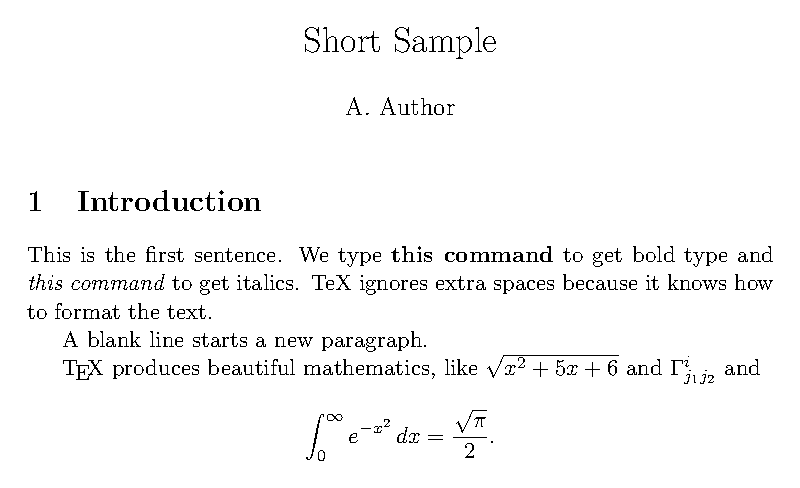
\includegraphics[width=0.85\hsize]{Graphics/manual-sample-output.pdf}}
   \label{fig:typeset}
\end{figure}
\capstarttrue

\section{\TeX\ and \LaTeX}
\label{LatexHistory}

\TeX\ was written by Donald Knuth at Stanford University and has been stable for decades. It understands a small
set of primitive commands and lets users combine them into new commands, called {\em macros}. A collection of macros
is a {\em format}. Knuth's own collection is plain \TeX; when people say they write in plain \TeX, they mean \TeX\
with these macros.

\LaTeX, originally written by Leslie Lamport, is a much larger collection of macros. It lets the author describe the
logical structure of a document (``this is a section title'', ``this is a theorem'') and leaves the layout to a
{\em document class} such as \texttt{article} or \texttt{book}. Thousands of {\em packages} extend it. The current
\LaTeX, called \LaTeXe, is maintained by the \LaTeX\ Project team, which improves it in regular releases while keeping
existing documents working.

The \TeX\ program has descendants that keep its typesetting but add modern abilities: pdf\TeX\ writes PDF files
directly, while Xe\TeX\ and Lua\TeX\ read Unicode source and use the OpenType fonts installed on the Mac. Each of them
can run \LaTeX; the result is called pdf\LaTeX, Xe\LaTeX\ or Lua\LaTeX. Choosing among them is explained in
\cref{chap:typesetting}.

\section{What TeXShop Does}

\TeX\ is a command line program, and most people use it through a front end: a program with an editing window for
the source, a command that runs \TeX, and a window that shows the result. TeXShop is such a front end for macOS. It is
free and open source; its source code is at \url{https://github.com/TeXShopProject/TeXShop}.

TeXShop does not typeset by itself. It runs the programs of a
\TeX\ distribution, normally TeX Live (see \cref{InstallingChapter}), and shows their output. Around this it offers
what makes writing \TeX\ comfortable on the Mac: syntax highlighting, command completion, macros, templates, spell
checking that knows \LaTeX, a Preview window synchronized with the source, and tools for projects with many files.

Many of these features are useful only after some experience with \LaTeX. There is no need to study them first:
\cref{GettingStartedChapter} describes what you need to begin, and the later chapters can be read as the need arises.

% ===== 02-installing.tex
\chapter{Installing TeX Live and TeXShop}\label{InstallingChapter}

To use \TeX\ on the Mac you need two things: a \TeX\ distribution, which contains the typesetting programs, fonts,
packages and documentation, and a front end such as TeXShop. TeXShop requires macOS 14.6 or later.

\section{TeX Live and MacTeX}
\label{TeXLiveSection}

The standard \TeX\ distribution is {\em TeX Live}. It is produced by the \TeX\ user groups for macOS, Windows, Linux
and other systems from the same sources, and a new version appears every year in spring. On the Mac it is
installed with an ordinary installer package from \url{https://tug.org/mactex/}, which offers two packages:

\begin{description}
\item[MacTeX] The complete TeX Live, together
with Ghostscript, and TeXShop and a few other applications in \path{/Applications/TeX}. With it almost any example
from a book about \TeX\ or \LaTeX\ works without adding anything. Choose this package for real work.
\item[BasicTeX] A small part of TeX Live, enough to try \TeX\ and to typeset many \LaTeX\ documents. It installs
neither TeXShop nor Ghostscript. If TeXShop reports that Ghostscript was not found, install Ghostscript too and
click \mnu{Detect Paths…} in \mnu{Settings}\To\mnu{Typesetting}\To\mnu{Paths}.
\end{description}

Double-click the downloaded package and follow the installer. When it ends, \TeX\ is ready to use.

MacTeX installs TeX Live in \path{/usr/local/texlive/2026}, and BasicTeX in \path{/usr/local/texlive/2026basic};
the folder is named after the year of the release. Several installations can exist side by side, and an installation
is removed by dragging its folder to the Trash. The installer also creates \path{/Library/TeX/texbin}, which always
leads to the programs of the TeX Live in use. TeXShop runs \TeX\ from there, so nothing has to be changed in TeXShop
when a new TeX Live is installed.

Between the yearly releases, the packages of TeX Live receive updates. MacTeX installs TeX Live Utility in
\path{/Applications/TeX} to install them.

TeXShop also works with \TeX\ installed in other ways, for example by MacPorts or Homebrew. Their programs are in
other folders; tell TeXShop where they are with \mnu{Detect Paths…} or by typing the folder in
\mnu{Settings}\To\mnu{Typesetting}\To\mnu{Paths}\To\mnu{TeX Engines} (see \cref{SettingsChapter}).

\section{Installing TeXShop}
\label{InstallingTeXShopSection}

MacTeX installs TeXShop in \path{/Applications/TeX}. TeXShop can also be downloaded from its web site,
\url{https://texshop.app/}; move the downloaded application to \path{/Applications} or \path{/Applications/TeX}.

MacTeX may contain an earlier version of TeXShop. After installing MacTeX, choose
\mnu{TeXShop}\To\mnu{Check for Updates...} once to bring TeXShop up to date. If no new version is offered, download
the current TeXShop from the web site and replace the copy in \path{/Applications/TeX}.

To open \texttt{.tex} files in TeXShop when they are double-clicked in the Finder, choose
\mnu{TeXShop}\To\mnu{Select TeXShop as Default TeX Editor}; macOS may ask you to confirm.

\section{The First Launch}
\label{FirstLaunchSection}

When TeXShop runs for the first time, it sets up two things in a row.

\begin{enumerate}
\item {\bf Paths.} TeXShop looks for the \TeX\ and Ghostscript installations on the Mac and lists them, newest first,
with the newest selected. Choose the one to use and click \mnu{OK}. The same search is available later as
\mnu{Detect Paths…} in \mnu{Settings}\To\mnu{Typesetting}\To\mnu{Paths}.
\item {\bf Engine profile.} TeXShop then shows \mnu{Choose an Engine Profile}. A profile sets up typesetting for
one engine in a single step; there are profiles for the common \LaTeX\ engines and for Japanese. Below the menu of
profiles, \mnu{Run LaTeX} chooses \mnu{Without latexmk} or \mnu{With latexmk}; \texttt{latexmk} repeats the
typesetting and runs Bib\TeX\ and the index program as needed. The list \mnu{Values to Set} shows what the chosen
profile will set. If unsure, keep the profile that is selected and click \mnu{OK}.
\end{enumerate}

Both choices can be changed at any time in \mnu{Settings}\To\mnu{Typesetting}; the profiles are described in
\cref{chap:typesetting}. On the first run TeXShop also creates the folder \path{~/Library/TeXShop} with its
templates, macros, engines and other files you can change (\cref{ConfiguringChapter}).

\section{Updating TeXShop}
\label{UpdatingTeXShop}

\mnu{TeXShop}\To\mnu{Check for Updates...} looks for a new version. When there is one, TeXShop shows what changed
and offers to install it, and then restarts.

The \mnu{Updates} category of Settings controls this:

\begin{description}
\item[Update to prereleases when available] TeXShop also offers prereleases (beta versions and release
candidates). A prerelease of TeXShop turns this on when it first runs; turn it off to receive only regular releases.
\item[Automatically check for updates] TeXShop looks for a new version by itself; \mnu{Check interval} sets how often
(daily, weekly or monthly).
\end{description}

The category also has a \mnu{Check for Updates...} button and shows when TeXShop last checked.

\mnu{TeXShop}\To\mnu{About TeXShop} shows the version in use; the link at the top of its credits opens the TeXShop
web site.

An update does not touch the files in \path{~/Library/TeXShop} that you may have edited, such as your macros and the
engines in use; \cref{LibraryUpdates} lists what it does renew. After an update, glance at
\mnu{Help}\To\mnu{About This Release}: it says when there is something to do by hand, which is usually nothing.
\mnu{Help}\To\mnu{Changes} lists what each version changed; the same list is on the web site.

% ===== 03-getting-started.tex
\chapter{Getting Started}\label{GettingStartedChapter}

This chapter takes you through a first document and the basic cycle of work: write, typeset, look at the result,
fix errors. It also shows the parts of the windows you work in. It is all you need to begin; the later chapters
describe each part in detail.

\section{A First Document}
\label{FirstDocumentSection}

\begin{enumerate}
\item Start TeXShop. An empty source window opens; if not, choose \mnu{File}\To\mnu{New}.
\item In the toolbar of the window, open the \mnu{Templates} menu and choose \mnu{LatexTemplate}. The window fills
with the lines that every \LaTeX\ document needs. Lines that start with \texttt{\%} are comments, which \TeX\ ignores.
\item Write some sentences between the lines
\begin{verbatim}
     \begin{document}
     \end{document}
\end{verbatim}
\TeX\ breaks the lines itself, so line breaks in the source do not matter. A blank line starts a new paragraph.
\item Click the \mnu{Typeset} button at the left end of the toolbar, or press \cmdkey-T
(\mnu{Typeset}\To\mnu{Typeset}).
\item The first time, TeXShop asks where to save the document. \TeX\ writes several auxiliary files next to the
source, so give each document a folder of its own: in the save dialog, go to a convenient place such as
\path{~/Documents}, click \mnu{New Folder}, and save the document inside the new folder under a meaningful name.
\item TeXShop runs \TeX\ and opens a Preview window with the typeset document.
\end{enumerate}

From then on the work is a cycle: change the source, press \cmdkey-T, look at the Preview. TeXShop saves the source
before every typesetting, and the Preview stays at the page you were reading. \cmdkey-T works in the source window,
the Preview and the console, and \mnu{Window}\To\mnu{Source ⇔ Preview} (\cmdkey-1) switches between the source and its
Preview.

Opening a \texttt{.tex} file also opens the PDF file of the same name, if there is one. Recently used documents are
listed in \mnu{File}\To\mnu{Open Recent}.

The Templates menu holds templates for other kinds of documents too, and \mnu{File}\To\mnu{New from Stationery...}
starts a new document from a complete sample; both are described in \cref{ConfiguringChapter}.

\section{The Parts of the Window}
\label{WindowPartsSection}

\Cref{fig:SourceAndPreview} shows a document with its source on the left and its Preview on the right. At first
TeXShop shows the source and the Preview in two windows; \cref{ArrangingWindowsSection} tells how to keep them in one
window, as in the figure. Either way, each part has the same toolbar items. Point to an item to see what it does.

\begin{figure}[htbp]
   \centering
   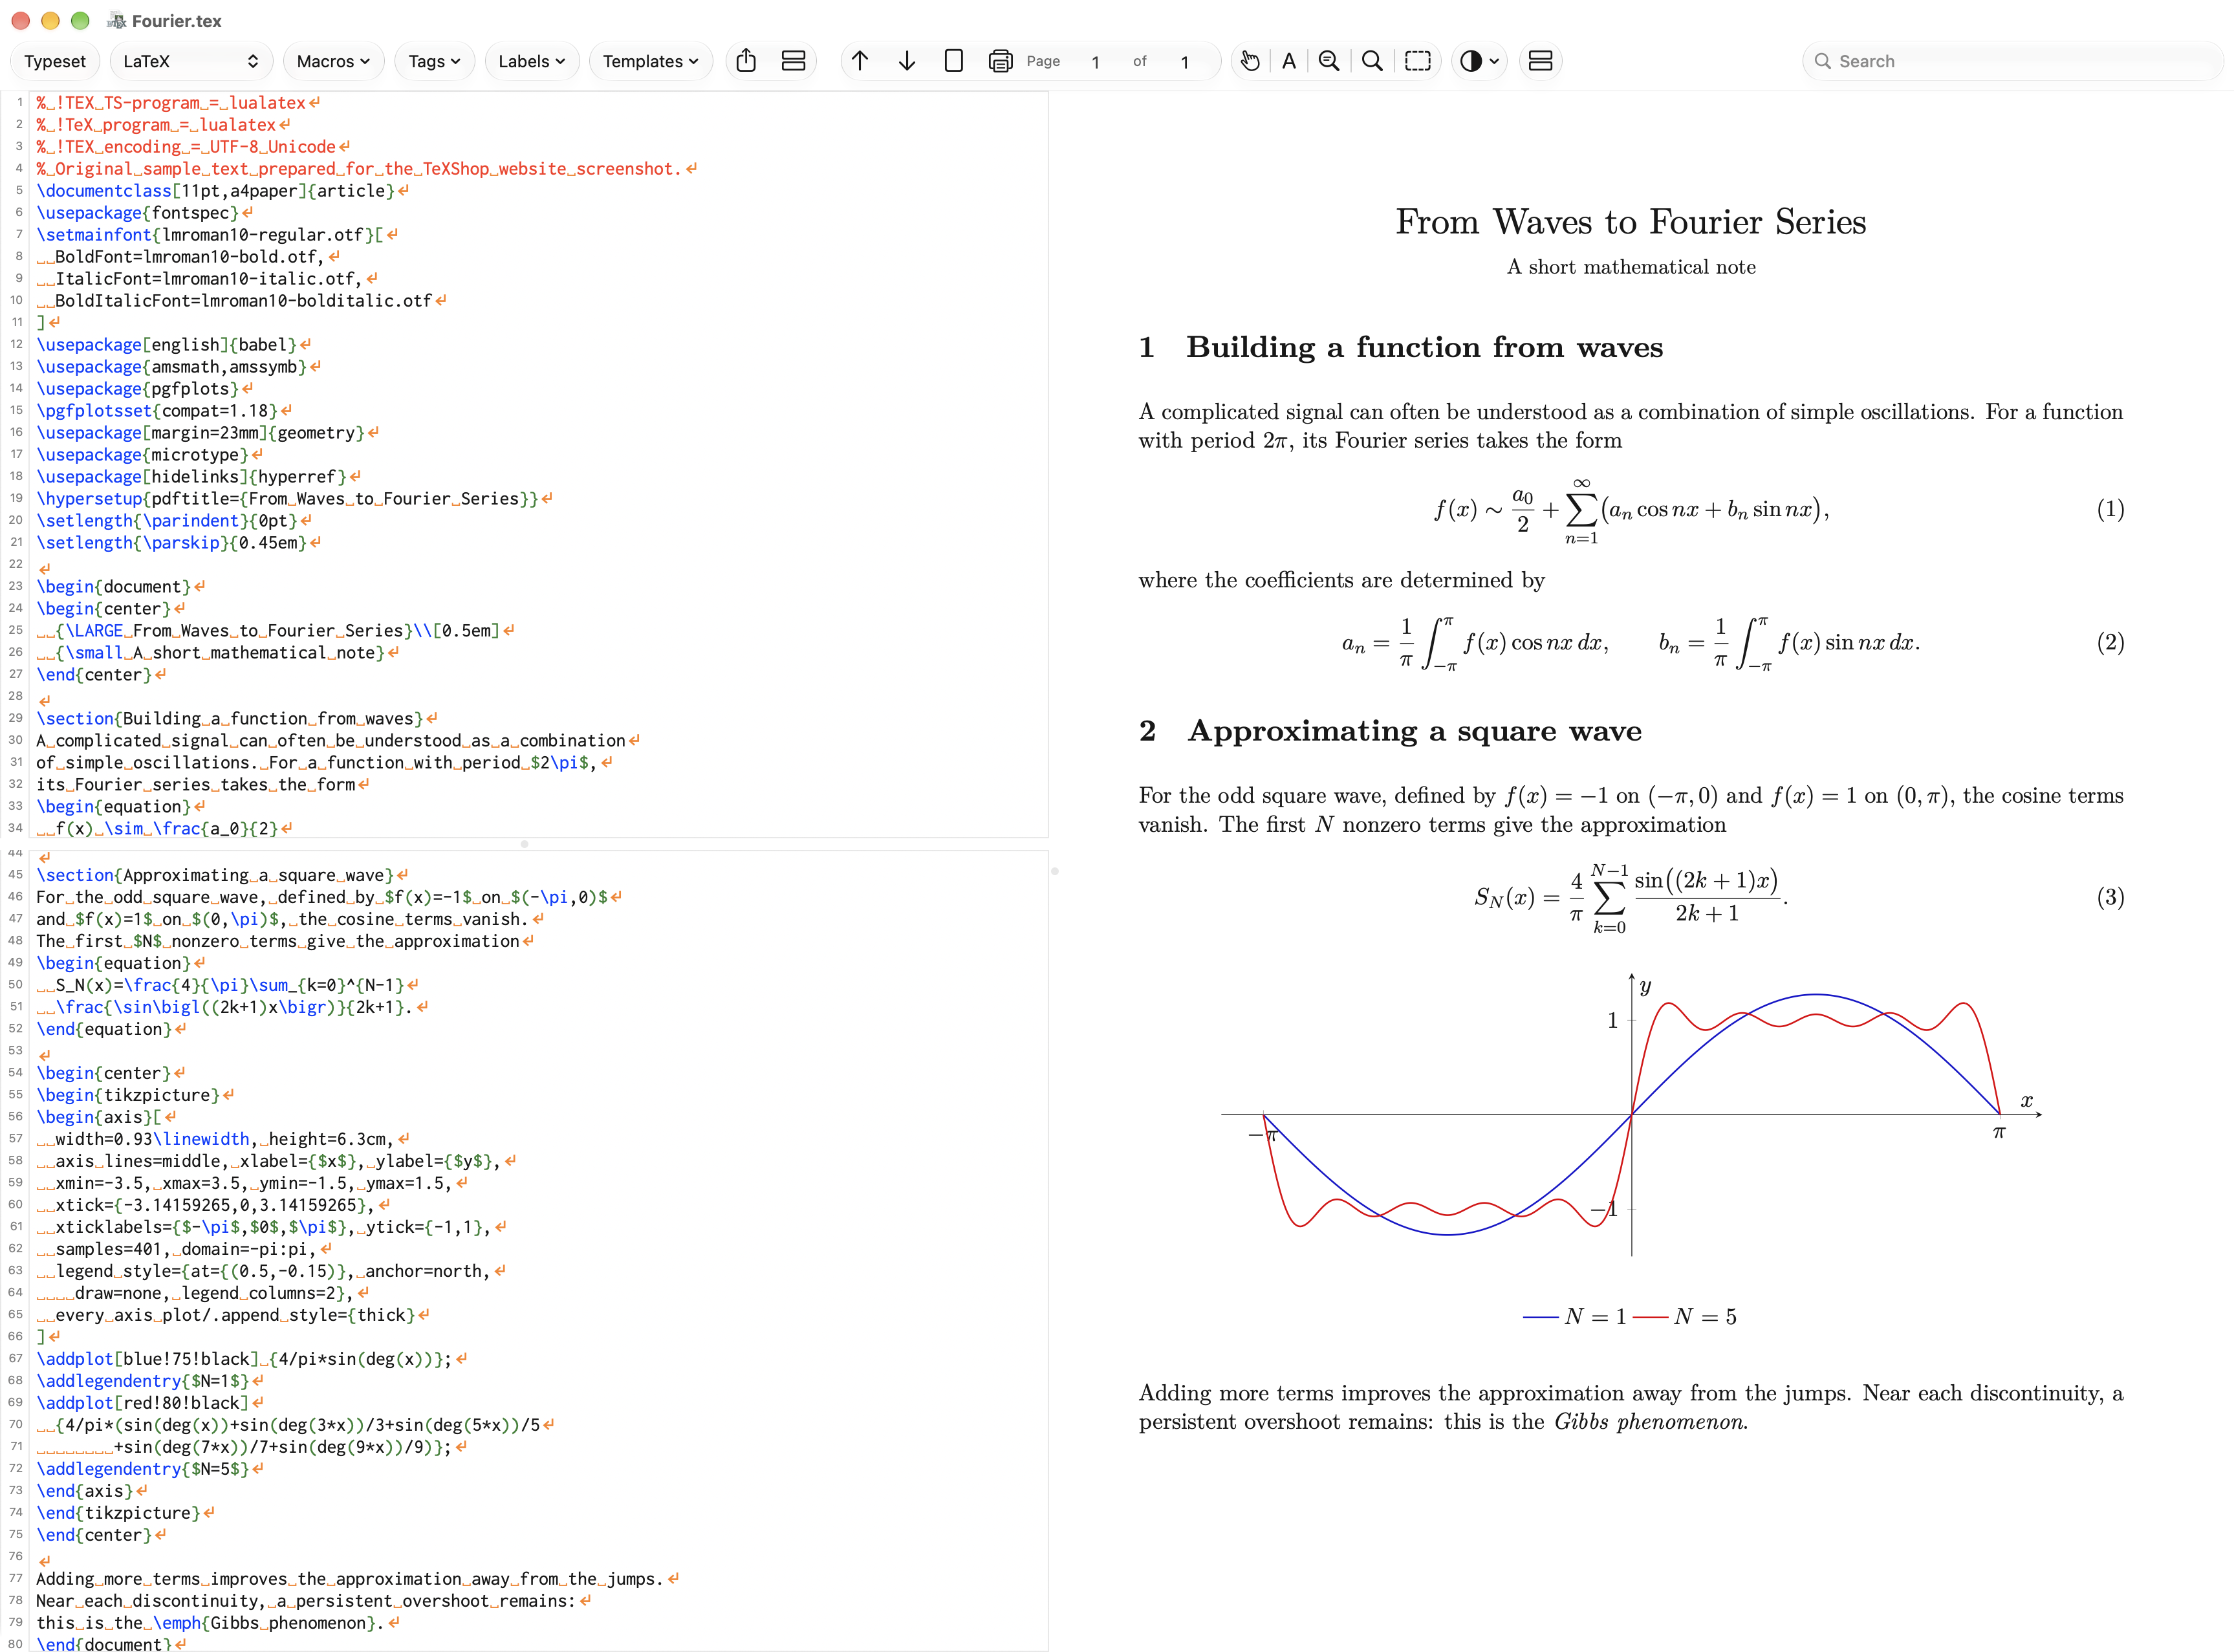
\includegraphics[width=\textwidth]{Graphics/manual-source-and-preview.png}
   \caption{A \LaTeX\ document in one window: the source with the status bar below it on the left, the Preview on the
   right, and the toolbar items of both above them}
   \label{fig:SourceAndPreview}
\end{figure}

\subsection{The Source}

You write in the source. Commands, comments and mathematics are shown in colors (\cref{ThemesChapter}). The line
numbers at the left side also select text: click a number to select that line, or drag over the numbers to select
several lines.

The toolbar above the source holds these items:
\begin{description}
\item[\mnu{Typeset}] The button at the left end. It typesets the document, like \cmdkey-T.
\item[\mnu{Program}] The menu next to it. It shows the program that \mnu{Typeset} runs, such as \mnu{LaTeX}, and
chooses another one for the window (\cref{sec:choosing-program}).
\item[\mnu{Macros}] Inserts often used commands and runs scripts (\cref{MacrosChapter}).
\item[\mnu{Tags}, \mnu{Labels}] Go to a section or to a \verb|\label| of the source (\cref{TagsSection}).
\item[\mnu{Templates}] Inserts a template (\cref{TemplatesSection}).
\item[\mnu{Share Source}] Shares the selected text, or the source file when nothing is selected, with the share
menu of macOS, for example by Mail.
\item[\mnu{Split Source}] Splits the source into two parts, to see two places of the document at once
(\cref{Splitting_Windows_Section}).
\end{description}

The status bar under the source shows the number of lines, characters and words in the document, and in the
selection when there is one; the location, line and column of the insertion point; and the size of the saved file.
Click \mnu{Text Statistics\ldots} in the status bar to count the words of the text without the \LaTeX\ commands
(\cref{CountingWordsSection}). \mnu{Source}\To\mnu{Show Status Bar} shows or hides the status bar.

\subsection{The Preview}

The Preview shows the typeset pages. Its toolbar holds these items:
\begin{description}
\item[\mnu{Previous}, \mnu{Next}] Turn the pages.
\item[\mnu{Go to page}] Shows the number of the page and the number of pages; type a number to go to that page.
\item[\mnu{Drawer}] Shows the outline of the document at the side of the Preview (\cref{Drawer_Section}).
\item[\mnu{Print}] Prints the document (\cref{PrintingSection}).
\item[\mnu{Mouse Mode}] Chooses what the pointer does on the page: move the page, select text, show a magnifying
glass, or select a part of the page to copy it as a picture (\cref{Preview_Mouse_Tools_Section}).
\item[\mnu{Appearance}] Shows the pages light or dark (\cref{PreviewAppearanceSection}).
\item[\mnu{Page Layout}] Shows one page or all pages in a scrolling column, single or in pairs
(\cref{DisplayFormatsSection}).
\item[\mnu{Two-Page Arrangement}] Sets the order of pages shown in pairs, and whether the first page stands alone
(\cref{TwoPageArrangementSection}).
\item[\mnu{Split Preview}] Splits the Preview into two parts.
\item[\mnu{Search PDF}] Finds text in the typeset document.
\end{description}
A separate Preview window also has \mnu{Back/Forward}, which returns to places you have visited
(\cref{Back_Forward_Arrows_Section}), and the \mnu{Magnification} field (\cref{MagnificationSection}).

\mnu{Window}\To\mnu{Customize Toolbar...} adds, removes and rearranges the items of the toolbar in front.

\subsection{The Console}

While \TeX\ runs, its messages appear in a third window, the console. \mnu{File}\To\mnu{Show Console} (\cmdkey-0)
brings it forward. It is described in the next section and in \cref{ConsoleSection}.

\section{Choosing the Engine}

TeXShop typesets with the engine set by the engine profile chosen at the first launch (\cref{FirstLaunchSection}).
To use another engine for a single document, put a line like this among the first lines of the source:
\begin{verbatim}
     % !TEX program = lualatex
\end{verbatim}
\cmdkey-T then always typesets that file with the named engine. The \mnu{Program} menu next to \mnu{Typeset} in the
toolbar chooses the engine for the window while it is open. See \cref{chap:typesetting} for the engines and profiles
and \cref{MagicCommentsChapter} for lines like this one.

\section{Errors}

While \TeX\ runs, its messages appear in the console. When \TeX\ finds an error, it shows a message at the end of the
console and waits for an answer: type it in the field at the bottom and press Return. Return alone goes on to the
next error. To stop \TeX, click \mnu{Abort} in the console or choose \mnu{File}\To\mnu{Abort Typesetting}.

\mnu{Edit}\To\mnu{Goto Error} (\ctlkey-\cmdkey-E), also a button in the console, shows the line of the first error in
the source; choose it again for the next one. One error often causes several more, so fixing the first few and
typesetting again is usually quickest.

\LaTeX\ keeps information between runs, such as cross-references and the table of contents, in auxiliary files; a
document may need two or three runs until every reference is right. An error can leave these files damaged, so that
the document fails even after the error is fixed. Then choose \mnu{Typeset}\To\mnu{Trash Aux \& Typeset}
(\optkey-\cmdkey-T), which moves the auxiliary files to the Trash and typesets again. See
\cref{sec:goto-error,sec:trash-aux} for more.

\section{Moving between Source and Preview}

\cmdkey-click a word in the source, and the Preview scrolls to the typeset text and marks it. \cmdkey-click in the
Preview, and the source comes forward with the matching text marked. The match is not always exact, so look around
the marked place. This uses SyncTeX, which the commands and engine files of TeXShop turn on; see
\cref{sec:synctex}.

\section{Arranging the Windows}
\label{ArrangingWindowsSection}

\mnu{Window}\To\mnu{Use One Window} puts the source and its Preview side by side in a single window, as in
\cref{fig:SourceAndPreview}, and \mnu{Window}\To\mnu{Use Separate Windows} separates them again. To open every
document this way, set \mnu{Settings}\To\mnu{General}\To\mnu{Source and Preview} to \mnu{Use One Window}. The divider
between the source and the Preview can be dragged; see \cref{OneWindowSection}.

With separate windows, place and size the source and Preview windows as you like, then choose
\mnu{Source}\To\mnu{Save Source Position} and \mnu{Preview}\To\mnu{Save Preview Position}; new windows open there.
The same positions can be set in \mnu{Settings}\To\mnu{General}\To\mnu{Window Positions}. Windows, tabs and splitting
are described in \cref{WindowsChapter}.

\section{Closing and Reopening}

Close a document with the close button of its window or \mnu{File}\To\mnu{Close} (\cmdkey-W). TeXShop saves documents
automatically (\cref{SavingChapter}), so nothing is lost. If you close only the Preview window, \cmdkey-1 or the next
typesetting opens it again at the page you were reading.

Whether documents left open when TeXShop quits reappear at the next start depends on macOS: they do when, in System
Settings \To\ Desktop \& Dock, ``Close windows when quitting an application'' is off.

\section{Hidden Menu Items: the Option Key}
\label{OptionKeyMenus}

Holding the Option key while a menu is open replaces some items with related ones, as in other Mac applications.
In TeXShop:

\begin{description}
\item[File menu] \mnu{Close} becomes \mnu{Close All}. When \mnu{Enable Autosave and Versions} is on in the
\mnu{Documents and Saving} category of Settings (the default), the File menu has \mnu{Duplicate}, and
\mnu{Save As...} appears in its place while Option is held.
\item[Typeset menu] \mnu{Typeset} becomes \mnu{Trash Aux \& Typeset} (\optkey-\cmdkey-T); with Control and Option it
becomes \mnu{Typeset with Alternate Engine}.
\item[Window menu] \mnu{Split Window} becomes \mnu{Split Window Vertically}, which places the two parts side by side.
\item[Edit menu] In \mnu{Marks}, \mnu{Next Mark} and \mnu{Previous Mark} become \mnu{Next Mark (Del)} and
\mnu{Previous Mark (Del)}, which also delete the mark.
\end{description}

\section{Text Substitutions}

macOS can replace straight quotes by curly ones, two hyphens by a dash, and words by their spelling corrections as
you type. In a \TeX\ source these changes break commands and quotation marks, so TeXShop turns them off in the source
window, whatever System Settings say. They can be turned on in \mnu{Edit}\To\mnu{Substitutions} and, for spelling
corrections, in \mnu{Settings}\To\mnu{Spell Checking}.

\section{Learning \LaTeX}

TeXShop helps you write \LaTeX; it does not teach it. Good starting points are:
\begin{itemize}
\item \url{https://www.learnlatex.org}, a series of short online lessons with examples that can be tried in the
browser;
\item {\em The Not So Short Introduction to \LaTeXe}, a free book of about 150 pages, at
\url{https://ctan.org/pkg/lshort-english};
\item the first part of George Grätzer's book {\em More Math Into \LaTeX}, included in TeXShop as
\mnu{Help}\To\mnu{George Grätzer's Short Course}\To\mnu{Short Course}; the same submenu opens the tables of math and
text symbols from the book.
\end{itemize}
\mnu{Help}\To\mnu{First Steps with TeXShop} is a short introduction to TeXShop itself. For questions while you write,
a precise web search, such as ``how to typeset a URL in LaTeX'', usually finds the answer.

% ===== 04-configuring.tex
\chapter{Configuring TeXShop}\label{ConfiguringChapter}

TeXShop keeps its configuration in two places. The choices made in the Settings window are stored by macOS in
TeXShop's settings file; they are described in \cref{SettingsChapter}. Templates, macros, engines, themes and other
files you can change are kept in the folder \path{~/Library/TeXShop}, described in this chapter.

\section{The Folder \texorpdfstring{\texttt{\textasciitilde/Library/TeXShop}}{\textasciitilde/Library/TeXShop}}
\label{LibraryTeXShopSection}

\path{~/Library/TeXShop} is the folder TeXShop in the Library folder of your home folder. Each user of the Mac has
their own. The Finder hides the Library folder; \mnu{TeXShop}\To\mnu{Open ~/Library/TeXShop} opens the folder in the
Finder. TeXShop creates it, with default contents, when it first runs.

Most of these files are changed from within TeXShop, for instance in the Macro Editor or in Settings, and need not be
opened by hand. The folders are:

\begin{description}[style=nextline]
\item[Templates] The templates of the \mnu{Templates} menu (\cref{TemplatesSection}).
\item[Stationery] The samples of \mnu{File}\To\mnu{New from Stationery...} (\cref{StationerySection}).
\item[Macros] The macros of the \mnu{Macros} menu, edited in the Macro Editor (\cref{MacrosChapter}).
\item[Engines] The engine files that appear in the engine menu of the toolbar; the subfolder \texttt{Inactive} holds
further engines that can be moved into \texttt{Engines} to use them (\cref{chap:engines}).
\item[Keyboard, CommandCompletion] The key bindings and the command completion list, edited in
\mnu{Settings}\To\mnu{Keyboard} (\cref{EditingChapter}).
\item[Menus] \texttt{KeyEquivalents.plist}, an older way to change menu shortcuts (\cref{KeyboardChapter}).
\item[LatexPanel, MatrixPanel] The contents of the LaTeX Panel and the Matrix Panel.
\item[Themes] The color themes, chosen and edited in \mnu{Settings}\To\mnu{Themes} (\cref{ThemesChapter}).
\item[SpellCheck] The rules for \LaTeX-aware spell checking, edited from \mnu{Settings}\To\mnu{Spell Checking}
(\cref{SpellCheckingChapter}).
\item[MultipleReplace] The saved sets of Multiple Replace (\cref{FindChapter}).
\item[HTML] Files for working with HTML (\cref{HTMLChapter}), among them the page shown by \mnu{Help}\To\mnu{HTML Commands}.
\item[ExternalEditorScripts] Scripts for working with an external editor (\cref{ExternalEditorChapter}).
\item[Documents] Additional documentation, for example about \texttt{latexmk} and command completion.
\item[New] Optional items that came with the current version of TeXShop (\cref{LibraryUpdates}).
\item[Backups] Damaged files that TeXShop has replaced (\cref{SelfRepairSection}). This folder appears only when needed.
\item[DraggedImages] Pictures dragged out of the Preview window are written here (\cref{CopyImagesSection}).
\item[Scripts, bin] Support files of TeXShop.
\end{description}
The file \texttt{About These Folders.rtf} in the folder describes the folders briefly.

\section{Templates}
\label{TemplatesSection}

The \mnu{Templates} menu in the toolbar of the source window inserts a template at the insertion point. TeXShop comes
with templates for the start of a plain \TeX\ document, a \LaTeX\ article, a Xe\LaTeX\ document, a \LaTeX\ article in Spanish and a Beamer
presentation, for including a graphic, for documents converted to HTML with \TeX4ht, and, in the submenu \mnu{More},
for preambles, document classes, floating figures and tables, and mathematical layouts.

Templates are ordinary \texttt{.tex} files, or \texttt{.typ} files for Typst (\cref{TypstChapter}), in
\path{~/Library/TeXShop/Templates}. Subfolders become submenus. Most
users soon make templates of their own, above all for the preamble of their articles: the packages and definitions
they always use. To make one, duplicate a template in the folder (for example \texttt{LatexTemplate.tex}), rename
the copy, and open it in TeXShop to change it; or save any \texttt{.tex} file into the folder. Templates you add,
rename or remove appear in the menu of windows opened afterward.

\section{Stationery}
\label{StationerySection}

\mnu{File}\To\mnu{New from Stationery...} starts a new document from a complete sample. Choose one in the list, which
shows a description of each, and click \mnu{OK}. The new document is untitled; save it where you like. TeXShop comes
with stationery for an AMS article, a Beamer presentation, a letter, a PreTeXt document, a project with a root file
and a chapter, and a Xe\LaTeX\ document.

The stationery is kept in \path{~/Library/TeXShop/Stationery}. To add your own, put the file there, for example
\texttt{Report.tex}, together with a plain text file \texttt{Report.comment} holding a sentence that describes it.
Every file in the folder except the \texttt{.comment} files is listed. New stationery appears in the list after
TeXShop is started again.

\section{What a New Version Changes}
\label{LibraryUpdates}

A new version of TeXShop leaves \path{~/Library/TeXShop} alone almost everywhere, so your changes are kept. A few
places hold TeXShop's own support files or optional items, and a new version brings them up to date:
\begin{itemize}
\item the folders \texttt{bin}, \texttt{Documents}, \texttt{ExternalEditorScripts} and \texttt{Scripts};
\item \texttt{Engines/Inactive} and \texttt{HTML/Inactive}, which hold engines and HTML files that you can move into use;
\item \texttt{HTML/Help.html}, the page shown by \mnu{Help}\To\mnu{HTML Commands};
\item the folder \texttt{New}, which is replaced as a whole.
\end{itemize}
In these places each file that comes with TeXShop is replaced by its new version, so changes you made to such a file
are lost; files you added under other names stay. To keep your own version of one of these files, save it under
another name.

The engines in use, in \texttt{Engines} itself, are never changed, since you may have edited them; only
\texttt{html.engine}, which \mnu{Help}\To\mnu{HTML Commands} needs, may be added there when it is missing. In
\texttt{Macros}, macros that came with TeXShop and were never edited may be updated to their current text; edited
macros and your own macros stay as they are. In \texttt{Themes}, colors of the themes that came with TeXShop that
you never changed may be updated to their current values; colors you changed and themes of your own stay as they
are.

The folder \texttt{New} contains items you may want to add yourself, such as new templates or engines. Move such an
item to the right folder and change it as you like. \mnu{Help}\To\mnu{About This Release} says when a version brings
something to pick up.

TeXShop updates these places once for each new version, not at every start, so an older version of TeXShop can be run
without changing the folder.

\section{Missing and Damaged Files}
\label{SelfRepairSection}

Some files in \path{~/Library/TeXShop} are needed for TeXShop to work: the LaTeX macros, the LaTeX Panel and Matrix
Panel files, the key bindings, the command completion lists, \texttt{KeyEquivalents.plist}, the themes \texttt{LiteTheme} and \texttt{DarkTheme}
and the themes in use, the spell checking rules, and \texttt{HTML/Help.html}. When TeXShop starts and finds one of
them missing or damaged, for instance after an editing mistake, it puts its own copy in place, without a message.
A damaged file is not deleted: it is moved to \path{~/Library/TeXShop/Backups}, into a folder named after the date
and time, so you can recover your changes from it.

A damaged theme of your own, or damaged macros of another engine, cannot be replaced by a copy from TeXShop; they too
are moved to \texttt{Backups}, and TeXShop uses its own theme or the LaTeX macros instead.

Templates, stationery, engines, scripts and your own themes are yours to delete: TeXShop does not bring them back,
except that a new version renews the places listed in \cref{LibraryUpdates}.

\section{Restoring Default Contents}
\label{RestoringDefaultsSection}

To get the default contents of a folder back, for instance \texttt{Templates} or \texttt{Macros}:
\begin{enumerate}
\item Quit TeXShop.
\item Move the folder out of \path{~/Library/TeXShop}, for example to the desktop.
\item Start TeXShop. It creates the folder again with its default contents.
\item Copy back from the moved folder whatever you want to keep.
\end{enumerate}
Removing single files does not bring them back (except the files listed in \cref{SelfRepairSection}); TeXShop
recreates only a folder that is missing as a whole.

\section{Resetting the Settings}
\label{ResettingSettings}

The settings are stored in \path{~/Library/Preferences/TeXShop.plist}. They are changed in the Settings window, and the
hidden settings with the \texttt{defaults} command in Terminal (\cref{chap:hidden-settings}); the file itself is
never edited by hand.

If TeXShop behaves strangely and you suspect its settings, you can start over with the factory settings. Quit
TeXShop, then in Terminal keep a copy of the current settings and remove them:
\begin{verbatim}
     defaults export TeXShop ~/Desktop/TeXShop-settings.plist
     defaults delete TeXShop
\end{verbatim}
Start TeXShop. It asks for the paths and the engine profile as on the first launch (\cref{FirstLaunchSection}); then
change in Settings what you had changed before. Menu shortcuts set in the \mnu{Keyboard} category of Settings are
settings too and return to their defaults. The folder \path{~/Library/TeXShop} is not affected, so key bindings,
command completion, themes and macros are kept.

To return to the settings you saved, quit TeXShop and type
\begin{verbatim}
     defaults import TeXShop ~/Desktop/TeXShop-settings.plist
\end{verbatim}
Use the \texttt{defaults} command rather than moving or replacing the file \texttt{TeXShop.plist}: macOS keeps the
settings in memory, and a file changed behind its back may be ignored or overwritten.

% ===== 05-settings.tex
\chapter{Settings}\label{SettingsChapter}

Choose \mnu{TeXShop}\To\mnu{Settings\ldots} (\cmdkey-,) to change how TeXShop works. The sidebar of the Settings window lists ten categories: General, Documents and Saving, Editor, Keyboard, Spell Checking, Themes, Typesetting, Console, Preview and Updates. Each category starts with a short overview and arranges its settings in named groups; on and off choices are switches, and most other choices are pop-up menus or fields. \Cref{fig:Settings} shows the General category. The sections below go through the categories in this order and give the main points of each group; the chapters they refer to describe the features themselves.

\begin{figure}[htbp]
   \centering
   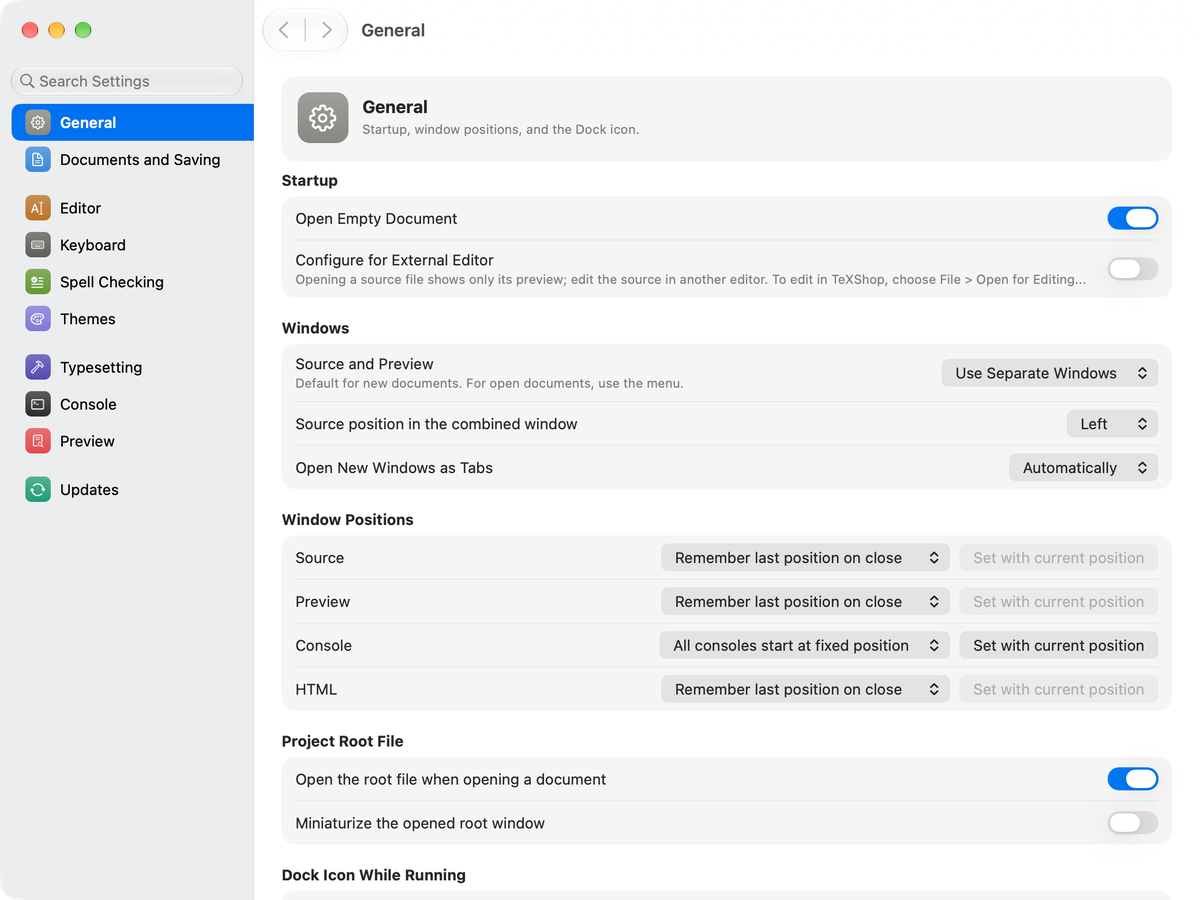
\includegraphics[width=0.9\textwidth]{Graphics/manual-settings.png}
   \caption{The General category of TeXShop Settings}
   \label{fig:Settings}
\end{figure}

Changes are saved as you make them. A text field takes its value when you press Return, move to another field, change the category or close the window. If the entry is not valid, TeXShop offers to correct it or to restore the value saved before.

The Back and Forward buttons at the top of the window, or \cmdkey-[ and \cmdkey-], return to the categories visited while Settings is open. When Settings opens again, it shows the category it showed last.

A few changes have consequences that are not visible at once. A short note with a yellow warning symbol then appears under the setting:
\begin{itemize}
\item a new \mnu{Magnification} in the Preview category applies to PDF files opened from then on; open previews keep their zoom;
\item a new \mnu{Encoding for new documents} does not change the encoding of documents that are already open;
\item \mnu{Enable Autosave and Versions}, and a switch of \mnu{Find interface} to or from the OgreKit Find Panel, take effect after TeXShop restarts.
\end{itemize}

\section{Settings and Menu Commands}\label{MenuDesign}

Several menu commands change the same behavior as a setting. The difference matters:
{\em a menu command changes only the active document, and only while it is open; a setting decides how documents start when they are opened.}

For example, \mnu{Source}\To\mnu{Show Line Numbers} shows or hides the line numbers of the active source window. Each window remembers its own state, and the menu item is checked or unchecked to match the window in front. The switch \mnu{Line Numbers} in the Editor category does not change any open window; it decides whether documents opened from then on show line numbers.

Most settings of this kind are gathered in the group \mnu{When a Document Opens}, at the top of the Editor category and of the Preview category. A few others are in other categories:
\begin{itemize}
\item \mnu{Source and Preview} in General, and \mnu{Window}\To\mnu{Use One Window} or \mnu{Use Separate Windows} for the active document;
\item \mnu{Typesetting Method} in Typesetting, and \mnu{Direct PDF}, \mnu{Via DVI} or \mnu{Personal Script} at the bottom of the \mnu{Typeset} menu;
\item \mnu{Typeset New Documents With} in Typesetting, and the pop-up menu beside the \mnu{Typeset} button in the toolbar;
\item \mnu{Use key bindings (default for new documents)} in Keyboard, and \mnu{Source}\To\mnu{Key Bindings}.
\end{itemize}

\section{Search Settings}\label{sec:SearchSettings}

Type in the field \mnu{Search Settings} at the top of the sidebar to find a setting, one of its choices, or a menu command (\cref{fig:SearchSettings}). Each result shows the name of the item and its category; select a result to go to the setting, which is briefly highlighted. Words separated by spaces must all describe the same item, and the name of a category among them narrows the search. Case, Latin accents, fullwidth characters and the difference between hiragana and katakana are ignored.

\begin{figure}[htbp]
   \centering
   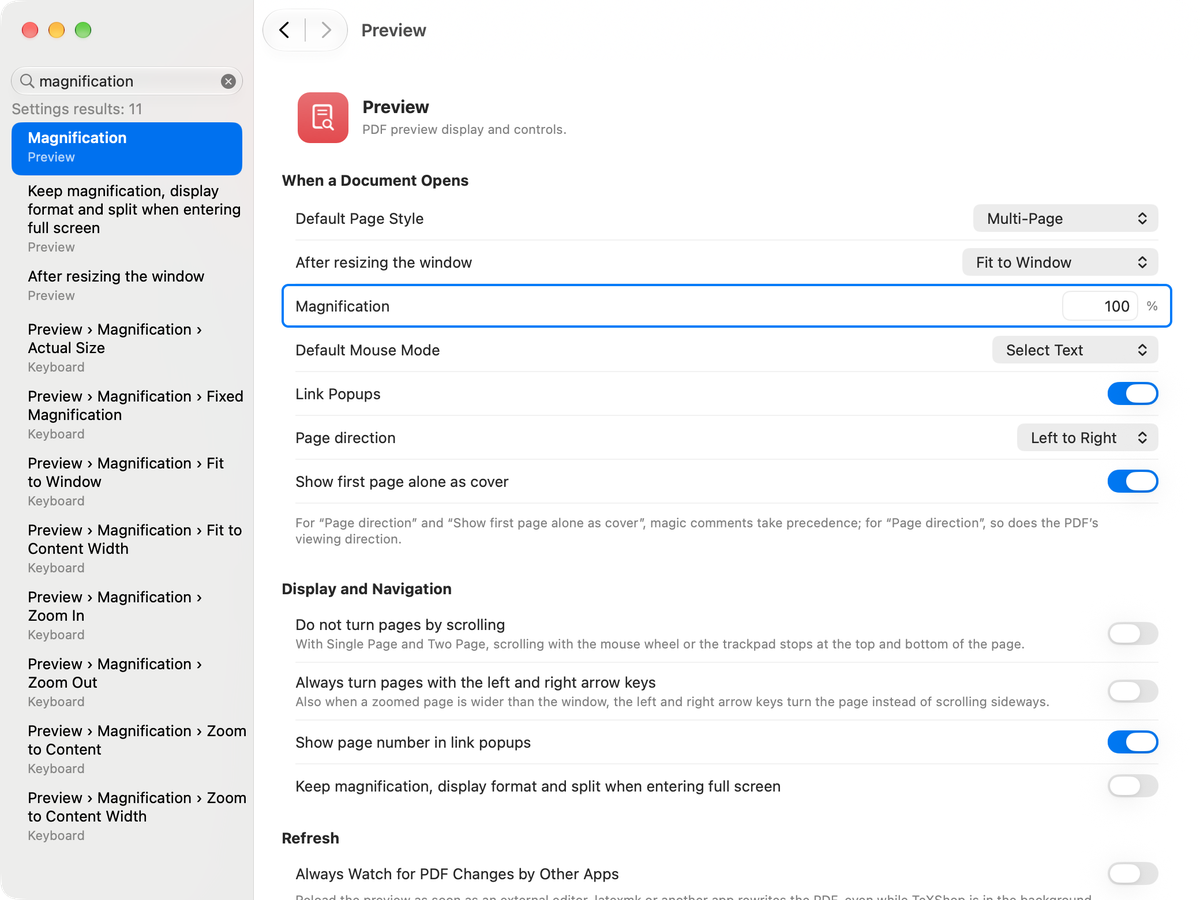
\includegraphics[width=0.9\textwidth]{Graphics/manual-settings-search.png}
   \caption{Search Settings with a word typed in the field; the results replace the list of categories}
   \label{fig:SearchSettings}
\end{figure}

Going to a result is a step in the history, so Back returns to where you were. A result for a menu command opens the Keyboard category with the command in the \mnu{Search by Function} field of the menu shortcut list, where its shortcut can be changed.

\section{General}\label{sec:SettingsGeneral}

{\bf Startup} With \mnu{Open Empty Document} on, TeXShop opens an empty document when it starts without a file. \mnu{Configure for External Editor} is for writing the source in another editor: opening a source file then shows only its preview. See \cref{ExternalEditorChapter}.

{\bf Windows} \mnu{Source and Preview} chooses whether new documents open in separate source and Preview windows or in one window, and \mnu{Source position in the combined window} puts the source on the left or the right of that window. For an open document, use \mnu{Use One Window} or \mnu{Use Separate Windows} in the \mnu{Window} menu. \mnu{Open New Windows as Tabs} is Never, Automatically or Always. See \cref{WindowsChapter}.

{\bf Window Positions} For each of the source, Preview, console and HTML windows, choose \mnu{Remember last position on close} or a fixed position. With a fixed position, \mnu{Set with current position} records the place and size of the window that is open now. \mnu{Source}\To\mnu{Save Source Position} and \mnu{Preview}\To\mnu{Save Preview Position} do the same from the windows themselves. If you usually work on one document, arrange its source and Preview windows side by side once and fix both positions.

{\bf Project Root File} \mnu{Open the root file when opening a document} opens the root file of a project, named by a \verb|% !TEX root| line, when one of its chapter files is opened; \mnu{Miniaturize the opened root window} puts that root window in the Dock. See \cref{chap:projects}.

\subsection{Dock Icon While Running}\label{sec:DockIcon}

\begin{figure}[htbp]
   \centering
   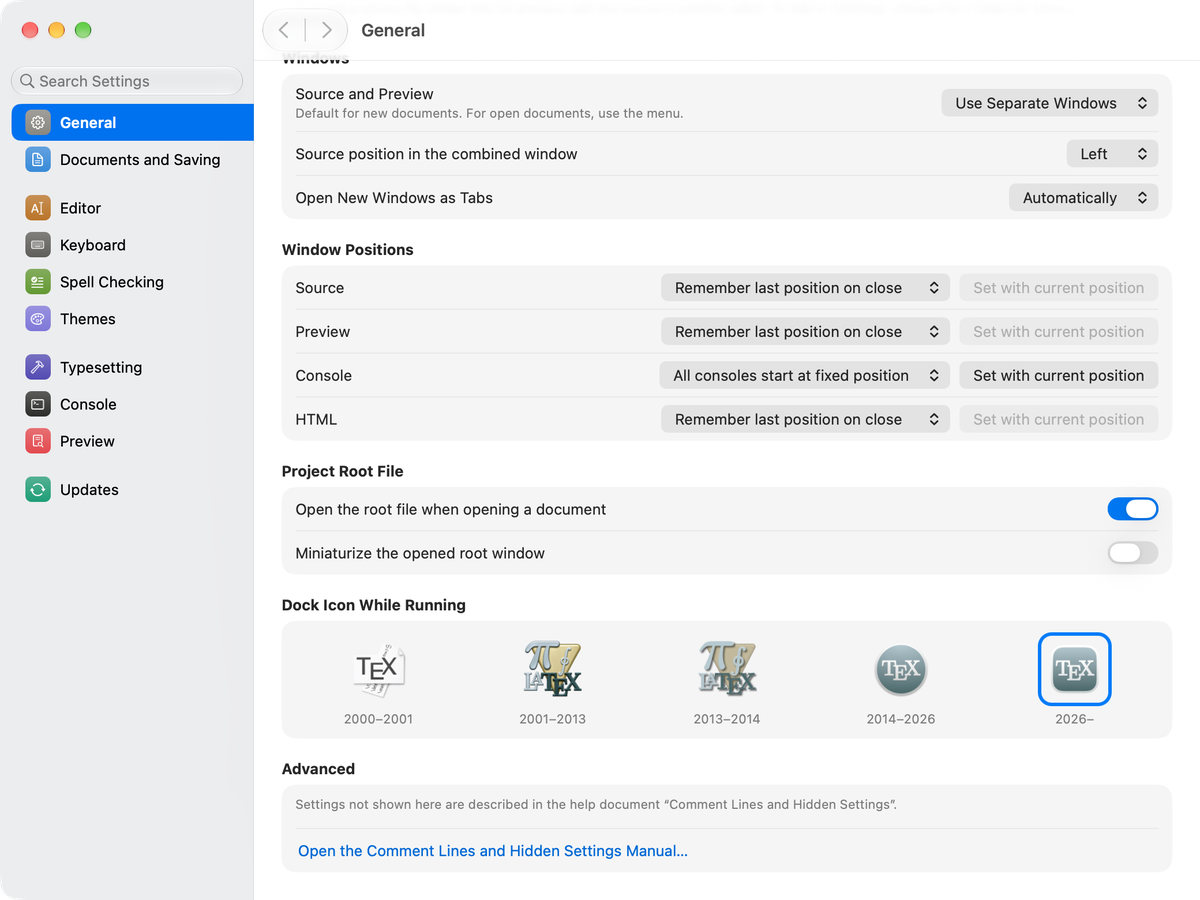
\includegraphics[width=0.9\textwidth]{Graphics/manual-dock-icons.png}
   \caption{Dock Icon While Running and Advanced, at the end of the General category}
   \label{fig:DockIcon}
\end{figure}

The group \mnu{Dock Icon While Running} (\cref{fig:DockIcon}) shows five icons: the current TeXShop icon, which is the default, and four earlier designs, each captioned with the years it was used. Click one to show it in the Dock. It is shown only while TeXShop is running; after TeXShop quits, the Dock shows the standard icon again, and the icon in the Finder never changes.

\subsection{Advanced}

Settings that are not shown in this window are hidden settings, changed with the \texttt{defaults} command in Terminal. The button \mnu{Open the Comment Lines and Hidden Settings Manual\ldots} in the group \mnu{Advanced} opens the document that lists them, together with the magic comment lines; the same document is in the Help menu as \mnu{Comment Lines and Hidden Settings}. See also \cref{MagicCommentsChapter,chap:hidden-settings}.

\section{Documents and Saving}\label{sec:SettingsDocuments}

{\bf Encoding} \mnu{Encoding for new documents} is \mnu{Unicode (UTF-8)} by default, the right choice for almost everyone. \mnu{Show Encoding in Save Dialog} adds an encoding menu to the Save dialog. See \cref{EncodingsChapter}.

{\bf Saving Documents} \mnu{Enable Autosave and Versions} turns on the macOS feature that saves documents while you edit them and keeps earlier versions; it is on by default, and a change takes effect after TeXShop restarts. \mnu{Keep the previous file as ``name\textasciitilde'' when saving} keeps a copy of the file as it was before each save, with a tilde before the extension: for \texttt{paper.tex} the copy is \texttt{paper\textasciitilde.tex}, and for \texttt{mystyle.sty} it is \texttt{mystyle\textasciitilde.sty}; it can be turned on while \mnu{Enable Autosave and Versions} is off. See \cref{SavingChapter}. \mnu{Automatically convert UTF-8-MAC to UTF-8} combines characters stored in separate parts, such as a kana and a separate voiced sound mark, into single characters when a document is saved.

\section{Settings for the Source Window}\label{sec:SettingsEditor}

The Editor category holds the settings of the source window: how it starts, its font and layout, typing aids, syntax highlighting, matching brackets, invisible characters, the block cursor, the Find interface and the XML tags of the Tags menu.

\subsection{When a Document Opens}

\mnu{Line Numbers}, \mnu{Highlight Current Line}, \mnu{Wrap Lines}, \mnu{Show Invisible Characters} and \mnu{Use Block Cursor} decide how new source windows start. The Source menu changes each of them for the active window, with \mnu{Show Line Numbers}, \mnu{Highlight Current Line}, the \mnu{Wrap Lines} submenu, \mnu{Show Invisible Characters} and \mnu{Use Block Insertion Cursor}.

\mnu{Wrap Lines} is \mnu{by Word} by default: a paragraph typed without line breaks is wrapped at the edge of the window, between words. The breaks are only for display and are not written to the file; they are recalculated when the window changes size. \mnu{by Character} may break inside words, and \mnu{None} does not wrap at all.

The current line is highlighted in the \mnu{Current Line} color of the theme. The block cursor colors the characters on each side of the insertion point; it replaces the highlighting of the current line while it is on. Its color and form are set in the group \mnu{Insertion} below. See \cref{BlockCursorSection}.

\subsection{Display}\label{Font_Size}

{\bf Document Font} To change the font in the Source Window, open the {\em Editor} category of Settings and click \mnu{Set\ldots} beside \mnu{Document Font}. Choose a font and size in the Font panel. The font applies to open and future source windows. A monospaced font keeps columns of source lined up. If you write in a script such as Hebrew or Arabic, choose a font that contains its letters; otherwise macOS substitutes another font for these characters, which can make editing long documents slow. The console has its own font, set in the Console category.

To enlarge or reduce the text of the active source window, use \mnu{Source}\To\mnu{Font}\To\mnu{Bigger} (\cmdkey-=) and \mnu{Smaller} (\cmdkey--). This changes only that window; \mnu{Document Font} stays as it is. If these shortcuts are inconvenient with your keyboard layout, assign others in the Keyboard category (\cref{sec:MenuShortcutKeystrokes}).

\mnu{Line Number Size} makes the line numbers in the left margin \mnu{Small} or \mnu{Large}. \mnu{Tags Menu in Menubar} adds the Tags menu of the toolbar to the menu bar.

\subsection{Style}

\mnu{Tab Size} is the width of a tab character, from 2 to 50 characters. \mnu{Use Tabs for Indent Menu} decides what \mnu{Source}\To\mnu{Indent} and \mnu{Unindent} insert and remove at the start of each selected line: a tab character, or as many spaces as Tab Size.

\mnu{Line Indent} and \mnu{Wrapped Line Indent} format paragraphs that are typed without line breaks: the first sets how far the first line of such a paragraph is indented, the second how far the lines after it are indented when the paragraph wraps. Both are 0 by default and range from 0 to 100 points. \mnu{Interline Spacing} sets the space between lines, from 1 to 20 points.

Only whole numbers can be entered; the arrow buttons beside each field raise or lower it by one, and a value outside the range is replaced by the nearest allowed value. Open source windows show a change as soon as the field takes its value, so you can try values until the text looks right.

\subsection{Typing}

\mnu{Select on Activate} decides what a click in a source window that is not in front does: with the switch on, the same click also moves the insertion point; with it off, the click only brings the window forward. With \mnu{Enclose selected text when typing a bracket} on, typing \verb|(|, \verb|[|, \verb|{| or \verb|$| while more than two characters are selected puts the pair around the selection instead of replacing it. \mnu{Right-to-left languages (Arabic, Hebrew, Persian)} aligns lines written in these scripts to the right; it works while syntax highlighting is on. See \cref{sec:RightToLeft}.

\subsection{Syntax Highlighting}

These switches change what syntax highlighting colors; the colors themselves are set in the Themes category.
\begin{description}
\item[@ as Part of Command Names] On by default: \texttt{@} counts as a letter of command names, as in the code of packages and classes.
\item[Highlight expl3 Code by Default] Documents open with expl3 code highlighted; \mnu{Source}\To\mnu{Highlight expl3 Code} changes it for the active window. See \cref{expl3Chapter}.
\item[Highlight Index Entries by Default] Documents open with the arguments of \verb|\index| and \verb|\esindex| shown in the Index color of the theme. \mnu{Source}\To\mnu{Highlight Index Entries} turns this on or off for the active source window. The setting also applies to the Macro Editor and the fields of the Advanced Find panel.
\item[Highlight Fullwidth Letters and Symbols] On by default: fullwidth letters, digits and symbols, and the minus sign, are shown in the Fullwidth colors of the theme.
\end{description}
Documents open with syntax highlighting on; \mnu{Source}\To\mnu{Syntax Highlighting} turns it off or on for the active window. To open documents with it off, set the hidden setting \texttt{SyntaxColoringEnabled} to \texttt{NO} (\cref{chap:hidden-settings}).

\subsection{Matching Brackets}\label{ParensPairs}

Clicking once in the source moves the insertion point there, a double click selects a word, and a triple click selects a paragraph. A double click on one of the brackets \verb|( ) [ ] { }| instead selects the bracket, its partner, and everything between them. This helps to find the cause of many \TeX\ errors.

When you type a closing bracket, TeXShop shows its partner, so you can check that the pairs in a formula match. The group \mnu{Matching Brackets} chooses how:
\begin{description}
\item[Parens Matching] On by default: the partner is briefly highlighted in yellow.
\item[Brackets] The pairs that are checked. The default \verb|{ }|, \verb|( )| and \verb|[ ]| work well; \verb|< >| is off because inequalities do not come in pairs.
\item[Highlight Enclosed Characters] The text between the pair is briefly painted in the Enclosed color of the theme. When the brackets are far apart, much of the window flashes.
\item[Blink Highlight] The partner blinks.
\item[Show Indicator in Moving] The partner is also shown in yellow when the insertion point moves next to a bracket, for instance with the arrow keys.
\item[Beep for Isolated Parens] A beep sounds when a closing bracket has no partner.
\item[Flash Back for Isolated Parens] The background of the window flashes in the Flash color of the theme when a closing bracket has no partner.
\end{description}

\subsection{Invisible}

\mnu{Source}\To\mnu{Show Invisible Characters} shows spaces, Japanese spaces, newlines and tabs in the active window, which helps when text behaves in a puzzling way. The group \mnu{Invisible} chooses which of these characters are shown and, in a pop-up menu beside each, the symbol used for it. Their color is Invisible in the Highlights group of the theme.

\subsection{Insertion}

\mnu{Cursor Color}, \mnu{Side of Insertion Line} and \mnu{Width for Left or Right} set the color of the block cursor, the side of the insertion point it covers, and how many characters it covers on that side.

\subsection{Find}

\mnu{Find interface} chooses the window or bar that the Find commands use. TeXShop offers four: \mnu{Advanced Find Panel (recommended)}, \mnu{Apple Find Panel}, \mnu{Apple Find Bar} and \mnu{OgreKit Find Panel (Legacy)}. Select each and try it. Switching among the Apple Find Panel, the Apple Find Bar and the Advanced Find Panel takes effect at once; switching to or from the OgreKit Find Panel takes effect after TeXShop restarts. The Advanced Find Panel finds with regular expressions, lists all matches, and replaces several pairs of strings at once; see \cref{FindChapter}.

The Advanced Find Panel normally takes its place among the document windows, so a click in a source window puts the panel behind it and Find brings it back. With \mnu{Keep the Advanced Find panel on top} on, the panel stays in front of the document windows.

\subsection{XML Tags in the Tag List}

For XML documents, such as PreTeXt sources, the Tags menu lists the elements checked in this group. Turn off the ones you do not need, so that the menu stays short. See \cref{XMLFeaturesSection}.

\section{Keyboard}\label{sec:SettingsKeyboard}

The Keyboard category sets what keys do in the source window and the shortcuts of the menu commands (\cref{fig:SettingsKeyboard}).

\begin{description}
\item[Key Bindings] \mnu{Use key bindings (default for new documents)} replaces a typed character by a text, such as \verb|{| by \verb|{}|; \mnu{Source}\To\mnu{Key Bindings} turns them on or off for the active document. The \mnu{Key Binding List} below the switch shows the replacements, where they can be added, changed and removed; check \mnu{Paste} for a replacement that should also apply to pasted text.
\item[Command Completion] \mnu{Completion trigger} chooses the key that completes the command you are typing; press it again for the next candidate, and with Shift for the previous one. \mnu{Move to the next or previous mark with Option or Control and the trigger key} adds mark navigation to that key, and \mnu{Edit Command Completion\ldots} opens the list of completions.
\item[Label and Citation Key Completion] \mnu{Edit}\To\mnu{Complete Label or Citation Key} offers the labels of the file after \verb|\ref{| and similar commands. With \mnu{Also offer BibDesk citation keys} on, it also offers BibDesk citation keys after \verb|\cite{| and similar commands.
\item[Menu Shortcuts] The list of all menu commands with their shortcuts, where any shortcut can be changed or removed. \mnu{Search by Function} finds a command by name, and \mnu{Search by Key} finds what a keystroke does. \mnu{Restore Default} and \mnu{Restore All\ldots} return to the default shortcuts.
\end{description}
See \cref{KeyBindingsSection,CommandCompletionSection,MarksSection,LabelCompletionSection,sec:MenuShortcutKeystrokes}.

\begin{figure}[htbp]
   \centering
   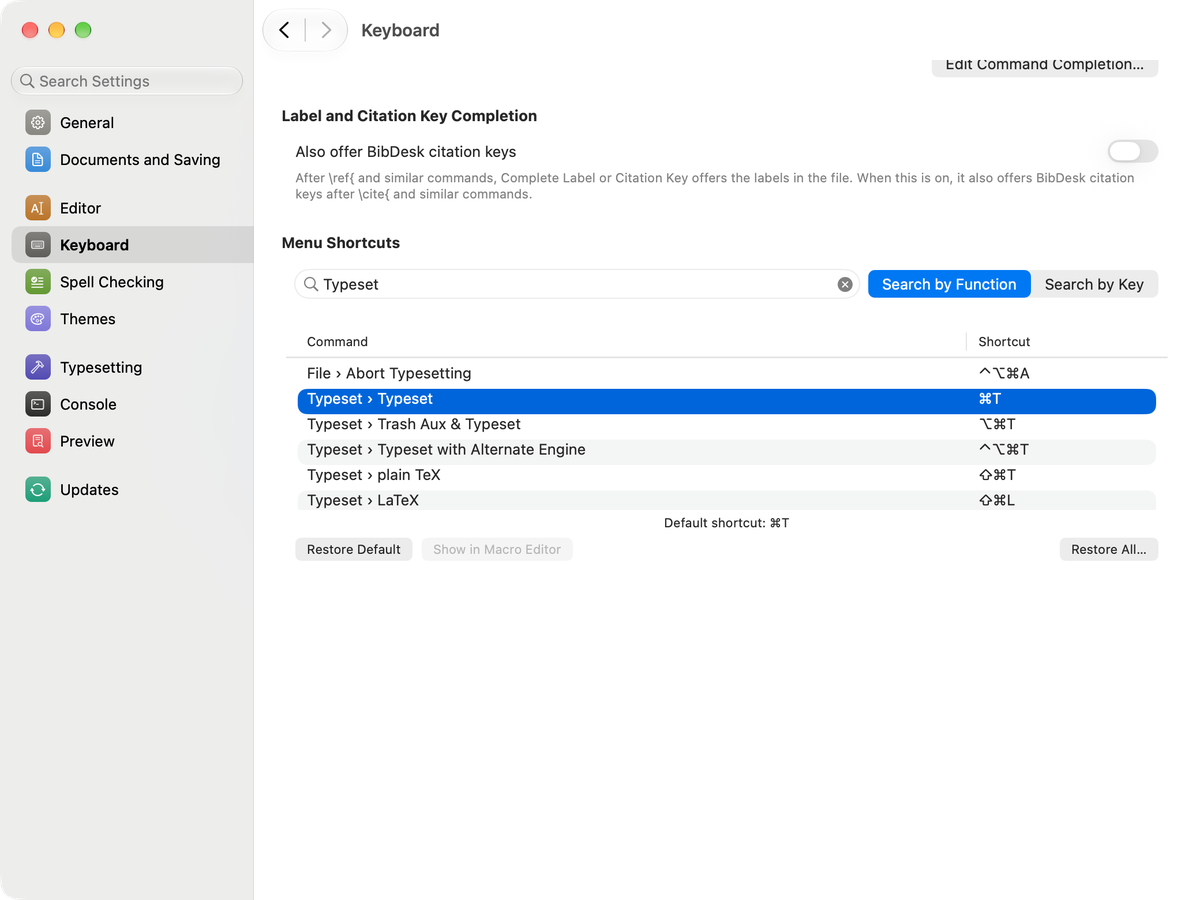
\includegraphics[width=0.9\textwidth]{Graphics/manual-settings-keyboard.png}
   \caption{The Menu Shortcuts group of the Keyboard category, searching by function}
   \label{fig:SettingsKeyboard}
\end{figure}

\section{Spell Checking}\label{sec:SettingsSpelling}

The group \mnu{Check Spelling} turns on \mnu{Check spelling while typing}, chooses whether macOS may correct words as you type (\mnu{Correct Spelling}), and chooses the \mnu{Dictionary}. \mnu{Correct Spelling} is off by default, so TeXShop does not correct words by itself even when other applications do.

Under \mnu{Method}, choose \mnu{Use LaTeX-aware spell checking (recommended)}, which leaves out commands, mathematics, comments and arguments such as those of \verb|\label| and \verb|\cite|; \mnu{Edit LaTeX exclusion rules\ldots} changes what it leaves out. \mnu{Legacy method} has three switches of its own: \mnu{Do not check LaTeX commands}, \mnu{Do not check selected parameters} and \mnu{Do not check comments}. See \cref{SpellCheckingChapter}.

\section{Themes}\label{sec:SettingsThemes}

A theme is a set of colors for the source, Preview, console and log windows, syntax highlighting, brackets, invisible characters and other highlights.
\begin{description}
\item[Themes] \mnu{Light Mode Theme} and \mnu{Dark Mode Theme} choose the theme used in each appearance of macOS.
\item[Edit Theme] The list of themes, where themes are added, duplicated, renamed, deleted, restored, exported and imported. The color groups below the list show the theme selected in it, and a change is saved at once.
\item[Color groups] \mnu{Windows} sets the text, background and opacity of the source, console, log and Preview windows; \mnu{Source} the insertion point, flash, current line and selection, where the insertion point and the selection can also follow the system color with \mnu{Use system color}; then come \mnu{Syntax Highlighting}, \mnu{Brackets}, \mnu{expl3}, \mnu{Highlights}, \mnu{SyncTeX}, \mnu{Color Mapping for Copied Images} and \mnu{XML Syntax}.
\end{description}
See \cref{ThemesChapter}.

\section{Typesetting}\label{sec:SettingsTypesetting}

The Typesetting category (\cref{fig:SettingsTypesetting}) is described in detail in \cref{chap:typesetting}; this section gives an overview.

\begin{figure}[htbp]
   \centering
   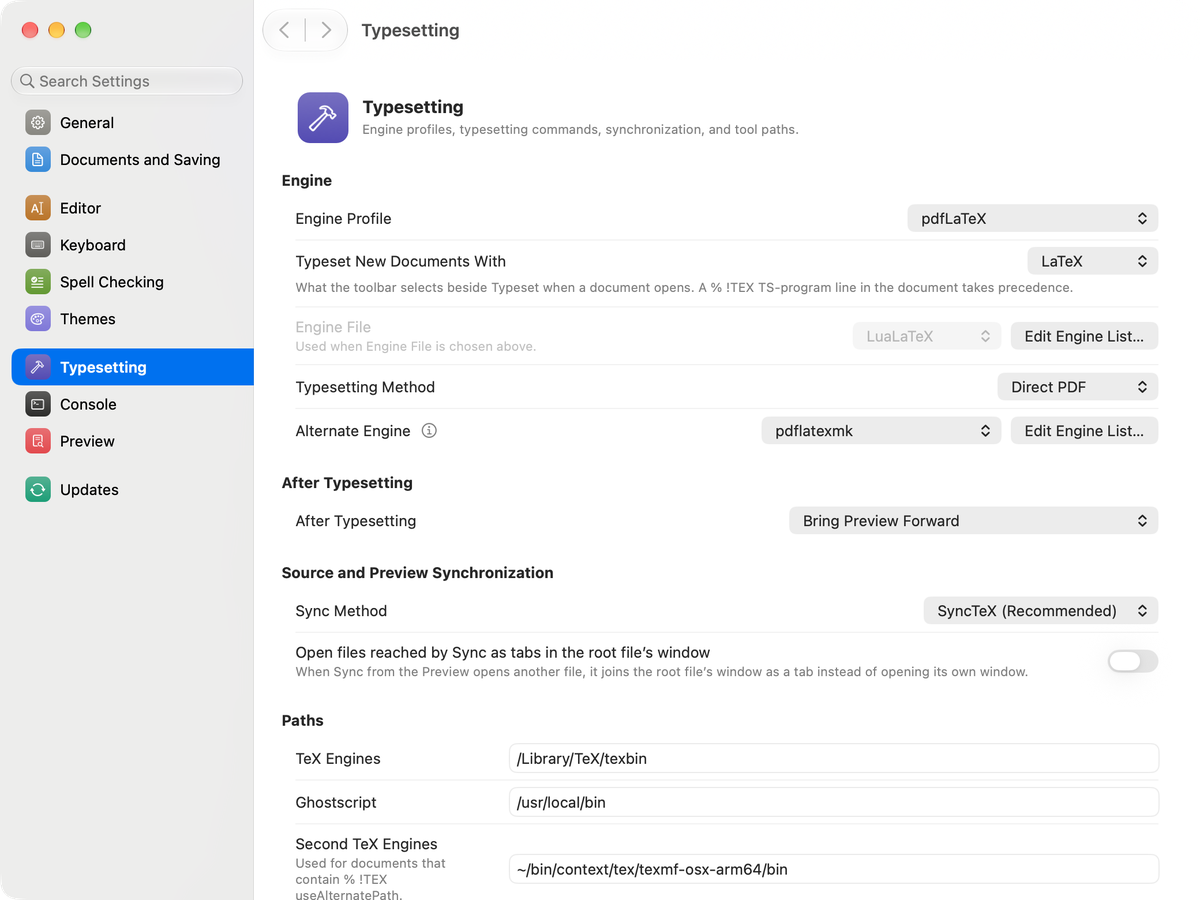
\includegraphics[width=0.9\textwidth]{Graphics/manual-settings-typesetting.png}
   \caption{The Engine, After Typesetting, Synchronization and Paths groups of the Typesetting category}
   \label{fig:SettingsTypesetting}
\end{figure}

{\bf Engine} \mnu{Engine Profile} sets up typesetting for one engine in one step; see below. \mnu{Typeset New Documents With} is what the toolbar selects beside the Typeset button when a document opens; a \verb|% !TEX program| line in the document takes precedence. \mnu{Engine File} is the engine used when Engine File is chosen there. \mnu{Typesetting Method} is Direct PDF, Via DVI or Personal Script, and \mnu{Alternate Engine} is the engine used by \mnu{Typeset}\To\mnu{Typeset with Alternate Engine}. The \mnu{Edit Engine List\ldots} buttons beside the two engine menus open the folder of engine files.

{\bf After Typesetting} chooses which window comes forward when typesetting ends: \mnu{Bring Preview Forward}, \mnu{Continue Editing}, or \mnu{Show Preview and Return to Original Window}.

{\bf Source and Preview Synchronization} \mnu{Sync Method} is \mnu{SyncTeX (Recommended)} or \mnu{Search PDF}. With \mnu{Open files reached by Sync as tabs in the root file's window} on, a file that a sync from the Preview window opens joins the window of the root file as a tab.

{\bf Paths} \mnu{TeX Engines} is the folder of the TeX programs, usually \texttt{/Library/TeX/texbin}, and \mnu{Ghostscript} the folder of Ghostscript. \mnu{Second TeX Engines} is a second folder of TeX programs, which engine files receive in place of TeX Engines for documents that contain \verb|% !TEX useAlternatePath|; the built-in plain \TeX\ and \LaTeX\ always use TeX Engines. \mnu{Detect Paths\ldots} looks for TeX Live and Ghostscript in the usual places, lists the installations it finds, newest first, and sets the one you choose.

{\bf Direct PDF, Via DVI, Personal Script} hold the plain \TeX\ and \LaTeX\ commands of each method. If a command of the Direct PDF group contains \texttt{-shell-escape}, turn on \mnu{Confirm Shell Escape} in that group to be asked before such a document is typeset; the commands of the other groups are not checked.

{\bf Related Tools} holds the commands for kpsewhich (used by \mnu{File}\To\mnu{Open Style File}), BibTeX, the index program and MetaPost. {\bf Japanese pLaTeX} has \mnu{Convert to otf Package \textbackslash UTF / \textbackslash CID}, described in \cref{JapanChapter}.

\subsection{Choosing an Engine Profile}\label{sec:EngineProfiles}

An engine profile sets all the commands that one way of typesetting needs. Choose a profile, such as pdfLaTeX, LuaLaTeX or upLaTeX + dvipdfmx, in the \mnu{Engine Profile} menu; a sheet lists the values it sets, and \mnu{OK} sets them. When the settings match no profile, the menu shows Custom. The profiles and the values they set are described in \cref{sec:configuring-typesetting}.

\section{Console}\label{sec:SettingsConsole}

{\bf Font} \mnu{Console Font} sets the font of the console; with \mnu{Use Also for Macro Editor} on, the Macro Editor uses it too.

{\bf Actions} \mnu{Show console} is \mnu{always}, so the console appears whenever typesetting starts, or \mnu{when error occurs}. \mnu{Console Resize} chooses whether the console can be resized freely or only vertically. Its position is set in the General category.

\section{Preview}\label{sec:SettingsPreview}

{\bf When a Document Opens} sets how new Preview windows show a document: the \mnu{Default Page Style} (Single Page, Two Page, Multi-Page or Double Multi-Page), what happens to the magnification \mnu{After resizing the window}, the \mnu{Magnification}, the \mnu{Default Mouse Mode}, whether \mnu{Link Popups} are shown, and, for two-page styles, the \mnu{Page direction} and \mnu{Show first page alone as cover}. Magic comment lines in a document take precedence over the last two (\cref{MagicCommentsChapter}), and the reading direction stored in a PDF file over the page direction.

{\bf Display and Navigation} \mnu{Do not turn pages by scrolling} keeps scrolling within the page in the Single Page and Two Page styles. \mnu{Always turn pages with the left and right arrow keys} makes these keys turn pages even when a zoomed page is wider than the window. \mnu{Show page number in link popups} and \mnu{Keep magnification, display format and split when entering full screen} do what they say.

{\bf Refresh} With \mnu{Always Watch for PDF Changes by Other Apps} on, the preview reloads as soon as another application, such as an external editor or latexmk, rewrites the PDF file, even while TeXShop is in the background.

{\bf Copy Images} \mnu{Image Copy Type} is the format of a selection copied or dragged from the Preview window as an image. With \mnu{Use Color Mapping} on, black in such an image becomes the text color and white the background color of the theme's group \mnu{Color Mapping for Copied Images}; PDF and EPS copies are not changed. Also with \mnu{Use Color Mapping} on, \mnu{Foreground Prominence} emphasizes text in raster copies.

{\bf HTML} \mnu{Home URL} is the web address or the file that the HTML window opens first.

See \cref{PreviewChapter}.

\section{Updates}\label{sec:SettingsUpdates}

{\bf Updates to Include} Turn on \mnu{Update to prereleases when available} to receive prereleases (beta versions and release candidates) too.

{\bf Automatic Checks} With \mnu{Automatically check for updates} on, TeXShop looks for a new version by itself, daily, weekly or monthly as chosen in \mnu{Check interval}. The switch is off by default.

At the bottom of the category, \mnu{Check for Updates\ldots} checks now and shows when TeXShop last checked. See \cref{UpdatingTeXShop}.

% ===== 06-typesetting.tex
\chapter{Typesetting}\label{chap:typesetting}

To typeset a document, press the \mnu{Typeset} button in the toolbar of the source window or type \cmdkey-T. The shortcut works in the source window, the Preview window and the console. TeXShop saves the source, runs the program chosen in the pop-up menu beside the \mnu{Typeset} button, shows its messages in the console and, when it ends, shows the new PDF file in the Preview window.

That pop-up menu lists plain \TeX, \LaTeX, BibTeX, MakeIndex, MetaPost and the engine files of \path{~/Library/TeXShop/Engines}. This chapter describes the built-in plain \TeX\ and \LaTeX, the settings that control them, and BibTeX, MakeIndex and MetaPost. Engine files, which typeset with any other program or chain of programs, are the subject of \cref{chap:engines}.

Which \TeX\ engine to use depends on the document. pdf\LaTeX\ is the classic choice. Xe\LaTeX\ and Lua\LaTeX\ read source written in any Unicode script and can use the OpenType fonts installed on the Mac; they also typeset almost all documents written for \LaTeX\ without changes.

\section{The Typeset Menu}\label{sec:typeset-menu}

\begin{center}
\begin{tabular}{lll}
\textbf{Item} & \textbf{Key} & \textbf{Action}\\ \hline
\mnu{Typeset} & \cmdkey-T & typeset the document\\
\mnu{Trash Aux \& Typeset} & \optkey-\cmdkey-T & trash aux files, then typeset\\
\mnu{Typeset with Alternate Engine} & \ctlkey-\optkey-\cmdkey-T & typeset with Alternate Engine\\
\mnu{plain TeX} & \shiftkey-\cmdkey-T & typeset with plain \TeX\\
\mnu{LaTeX} & \shiftkey-\cmdkey-L & typeset with \LaTeX\\
\mnu{BibTeX} & \shiftkey-\cmdkey-B & run BibTeX\\
\mnu{MakeIndex} & \shiftkey-\cmdkey-I & run MakeIndex\\
\mnu{MetaPost} & \shiftkey-\cmdkey-M & run MetaPost\\
\mnu{Direct PDF} & & method of this document\\
\mnu{Via DVI} & & method of this document\\
\mnu{Personal Script} & & method of this document\\
\end{tabular}
\end{center}

\mnu{Trash Aux \& Typeset} appears in place of \mnu{Typeset} while you hold down Option, and \mnu{Typeset with Alternate Engine} while you hold down Control and Option. The keys are those TeXShop comes with; they can be changed in \mnu{Settings}\To\mnu{Keyboard}.

\mnu{Typeset} uses the program that the document asks for in a \verb|% !TEX program| line, or else the program chosen in the toolbar. The items \mnu{plain TeX}, \mnu{LaTeX} and \mnu{MetaPost} ignore such a line: they choose that program in the toolbar and run it. \mnu{BibTeX} and \mnu{MakeIndex} run their programs without changing the toolbar. \mnu{Trash Aux \& Typeset} is explained in \cref{sec:trash-aux}, and \mnu{Typeset with Alternate Engine} in \cref{sec:latexmk}.

\section{Engine Profiles}\label{sec:configuring-typesetting}

The quickest way to set up typesetting is an engine profile. In \mnu{Settings}\To\mnu{Typesetting}, choose a profile in the \mnu{Engine Profile} pop-up menu at the top of the \mnu{Engine} group. The menu has three sections:
\begin{itemize}
\item pdfLaTeX, XeLaTeX, LuaLaTeX and LaTeX + dvipdfmx;
\item for Japanese, LuaLaTeX (Japanese), upLaTeX + dvipdfmx and pLaTeX + dvipdfmx;
\item under \mnu{Other}, LaTeX + dvips + Ghostscript.
\end{itemize}

A sheet then lists, under \mnu{Values to Set}, the values the profile sets and marks each one that changes with a checkbox; turn a value off to keep the current setting (\cref{fig:EngineProfileSheet}). \mnu{Run LaTeX} chooses \mnu{Without latexmk}, so that each typesetting runs the engine once, or \mnu{With latexmk}, so that latexmk runs BibTeX, the index and further passes as needed. \mnu{OK} sets the profile, and \mnu{Cancel} leaves every setting as it was.

\begin{figure}[htbp]
   \centering
   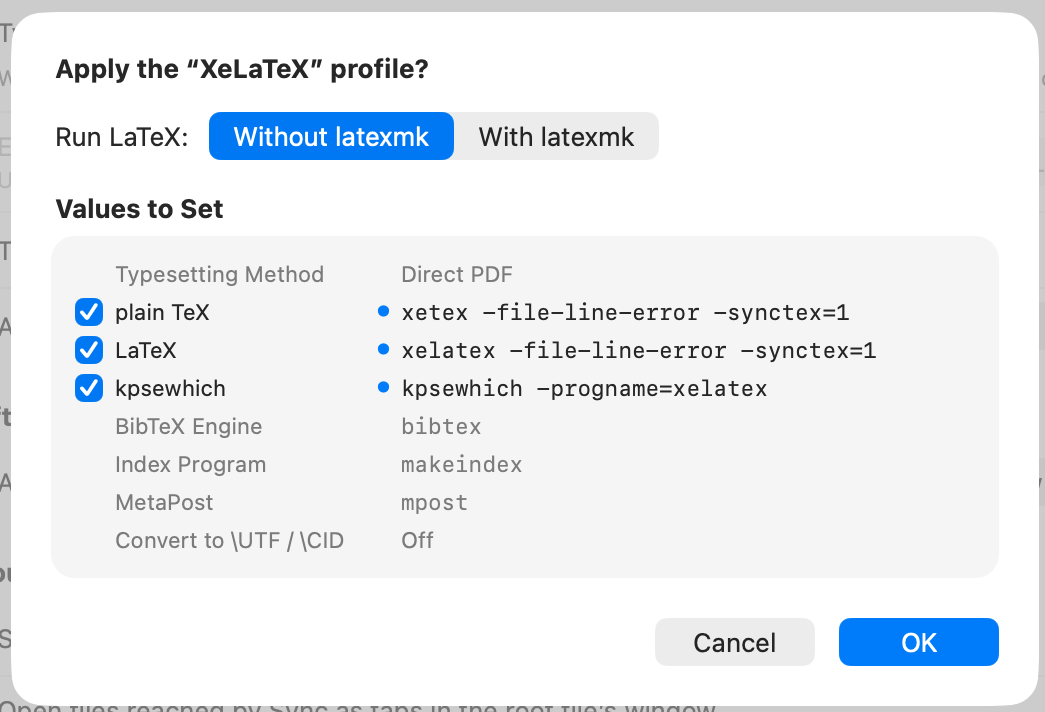
\includegraphics[width=0.6\textwidth]{Graphics/manual-engine-profile.png}
   \caption{The sheet shown after choosing an engine profile}
   \label{fig:EngineProfileSheet}
\end{figure}

The menu shows the profile all of whose values are set now, or \mnu{Custom} as soon as any of these values is changed, in Settings or elsewhere. To return to the values of a profile, choose it again, even when the menu shows it.

When TeXShop starts for the first time, it asks for the paths to \TeX\ and Ghostscript (see \cref{sec:typesetting-paths}) and then for an engine profile. It suggests upLaTeX + dvipdfmx when Japanese is the first preferred language of macOS, and pdfLaTeX otherwise.

\subsection{What a Profile Sets}

A profile sets the typesetting method and the plain \TeX\ and \LaTeX\ commands of that method (\cref{sec:direct-pdf-via-dvi}). The commands of the other method are not changed.

For each profile, the method and the \LaTeX\ and plain \TeX\ commands are:
{\small
\begin{verbatim}
pdfLaTeX                                     Direct PDF
  pdflatex -file-line-error -synctex=1
  pdftex -file-line-error -synctex=1
XeLaTeX                                      Direct PDF
  xelatex -file-line-error -synctex=1
  xetex -file-line-error -synctex=1
LuaLaTeX, LuaLaTeX (Japanese)                Direct PDF
  lualatex --file-line-error --synctex=1
  luatex --file-line-error --synctex=1
LaTeX + dvipdfmx                             Via DVI
  simpdftex latex --mode dvipdfmx --extratexopts "-file-line-error -synctex=1"
  simpdftex etex --mode dvipdfmx --extratexopts "-file-line-error -synctex=1"
upLaTeX + dvipdfmx                           Via DVI
  ptex2pdf -u -l -ot "-synctex=1 -file-line-error"
  ptex2pdf -e -u -ot "-synctex=1 -file-line-error"
pLaTeX + dvipdfmx                            Via DVI
  ptex2pdf -l -ot "-synctex=1 -file-line-error"
  ptex2pdf -e -ot "-synctex=1 -file-line-error"
LaTeX + dvips + Ghostscript                  Via DVI
  simpdftex latex --maxpfb --extratexopts "-file-line-error -synctex=1"
  simpdftex etex --maxpfb --extratexopts "-file-line-error -synctex=1"
\end{verbatim}
}

With latexmk, the \LaTeX\ command becomes a call of latexmk that runs the same engine with \verb|-synctex=1| and \verb|-file-line-error| and with \verb|-norc|, so that no personal latexmk configuration file changes it. For the pdfLaTeX profile it reads
{\small
\begin{verbatim}
     latexmk -pdf -e "$pdflatex=q/pdflatex -synctex=1 -file-line-error/" -norc
\end{verbatim}
}
The latexmk commands of the Japanese profiles also name the BibTeX and index programs of the profile.

The profiles also set the tools of the \mnu{Related Tools} group:

\begin{center}
\begin{tabular}{llll}
\textbf{Profile} & \textbf{BibTeX Engine} & \textbf{Index Program} & \textbf{MetaPost}\\ \hline
pdfLaTeX, XeLaTeX, LuaLaTeX & bibtex & makeindex & mpost\\
LaTeX + dvipdfmx & bibtex & makeindex & mpost\\
LaTeX + dvips + Ghostscript & bibtex & makeindex & mpost\\
LuaLaTeX (Japanese) & upbibtex & upmendex & mpost\\
upLaTeX + dvipdfmx & upbibtex & upmendex & upmpost\\
pLaTeX + dvipdfmx & pbibtex & mendex & pmpost\\
\end{tabular}
\end{center}

The \mnu{kpsewhich} command, which \mnu{File}\To\mnu{Open Style File} uses to find a file, becomes \verb|kpsewhich -progname=| followed by \verb|latex|, \verb|xelatex|, \verb|lualatex|, \verb|platex| or \verb|uplatex|, according to the profile; for example, the XeLaTeX profile sets \verb|kpsewhich -progname=xelatex|. The pLaTeX + dvipdfmx profile turns on \mnu{Convert to otf Package \textbackslash UTF / \textbackslash CID} in the \mnu{Japanese pLaTeX} group, and every other profile turns it off. The Japanese profiles also set UTF-8 as the encoding of new documents, set the spelling dictionary to automatic language detection, and turn on UTF-8-MAC conversion. Every other setting stays as it is.

\section{Choosing the Program}\label{sec:choosing-program}

When a document opens, the toolbar selects the program chosen in the \mnu{Typeset New Documents With} pop-up menu of \mnu{Settings}\To\mnu{Typesetting}: \mnu{plain TeX}, \mnu{LaTeX} (the default), or \mnu{Engine File}. With \mnu{Engine File}, the \mnu{Engine File} pop-up menu below it chooses the engine; LuaLaTeX is chosen at first. That menu lists the engine files in \path{~/Library/TeXShop/Engines}. \mnu{Edit Engine List\ldots} opens this folder in the Finder, where you can add, remove or rename engine files; the menu follows the folder. If the engine file of the setting is no longer in the folder, the menu shows it as not found, and documents are typeset with \LaTeX\ instead.

To change the program of one document, choose another program in the toolbar; the choice holds for that window. To tie a document to a program, put a line such as
\begin{verbatim}
     % !TEX program = pdflatex
\end{verbatim}
in one of its first twenty lines. The form \verb|% !TEX TS-program =| is read the same way. Such a line takes precedence over the toolbar and the settings. Besides the names of engine files, it accepts these names for the built-in programs:

\begin{center}
\begin{tabular}{ll}
\verb|pdflatex| & \LaTeX, Direct PDF\\
\verb|latex| & \LaTeX, Via DVI\\
\verb|personallatex| & \LaTeX, Personal Script\\
\verb|pdftex| & plain \TeX, Direct PDF\\
\verb|tex| & plain \TeX, Via DVI\\
\verb|personaltex| & plain \TeX, Personal Script\\
\verb|bibtex| & BibTeX\\
\verb|makeindex| & MakeIndex\\
\verb|metapost| & MetaPost\\
\end{tabular}
\end{center}

Do not give an engine file one of these names. \Cref{sec:typesetting-with-engine} says more about the line and the \mnu{Program} macro that writes it.

\section{Direct PDF and Via DVI}\label{sec:direct-pdf-via-dvi}

The built-in plain \TeX\ and \LaTeX\ typeset with one of three methods:
\begin{description}
\item[Direct PDF] runs a program that writes the PDF file directly, such as pdflatex. Most documents are typeset this way.
\item[Via DVI] runs \TeX\ to write a DVI file and converts it to PDF. With the factory commands, the script simpdftex of \TeX\ Live runs \LaTeX, converts the DVI file to PostScript with dvips and the PostScript to PDF with Ghostscript. This method is needed for documents that put PostScript code into the output, for instance with the pstricks package. EPS pictures do not need it: \TeX\ Live converts them to PDF while typesetting Direct PDF. The Japanese profiles use this method with dvipdfmx, which converts DVI to PDF directly.
\item[Personal Script] runs the commands of the \mnu{Personal Script} group, for those who want a command of their own; while a command there is empty, the Direct PDF command is used.
\end{description}

\mnu{Settings}\To\mnu{Typesetting}\To\mnu{Typesetting Method} sets the method that documents start with. To switch the method of one document, choose \mnu{Direct PDF}, \mnu{Via DVI} or \mnu{Personal Script} at the bottom of the \mnu{Typeset} menu. This affects only the active document, so two open documents can use different methods.

\subsection{The Commands}

The \mnu{Direct PDF}, \mnu{Via DVI} and \mnu{Personal Script} groups of \mnu{Settings}\To\mnu{Typesetting} hold the command of each method, one for plain \TeX\ and one for \LaTeX. TeXShop runs the command in the folder of the source file with the name of the file added, just as you would in Terminal:
\begin{verbatim}
     pdflatex -file-line-error -synctex=1 Galois.tex
\end{verbatim}

The two options of the factory commands are important. With \verb|-file-line-error|, \TeX\ reports each error with the name of its file and its line, which \mnu{Goto Error} uses (\cref{sec:goto-error}). With \verb|-synctex=1|, \TeX\ writes the information that synchronizes the source and the Preview window (\cref{sec:synctex}). The pdftex defaults use two flags, written with one hyphen as in the usage of pdftex; LuaTeX writes them with two (\verb|--file-line-error|), and every engine accepts either form.

\subsection{Shell Escape}

The option \verb|-shell-escape| lets \TeX\ run other programs while it typesets; some packages need it. A document typeset with this option can run any command, even one that erases your home folder, so add it only for documents you trust. If you add it to a command of the \mnu{Direct PDF} group, consider turning on \mnu{Confirm Shell Escape} in that group. TeXShop then asks before it first typesets a document after opening it: \mnu{OK} typesets with the option, \mnu{Omit Shell Escape} typesets without it, and \mnu{Cancel} does not typeset. The answer holds for that document until it is closed. TeXShop recognizes the option written with one or two hyphens; engine files are not checked.

\subsection{Options for Via DVI}

Ghostscript ignores PostScript transparency by default. To keep it, add the following to the end of the plain \TeX\ or \LaTeX\ command in the \mnu{Via DVI} group; simpdftex passes it to Ghostscript.
\begin{verbatim}
     --distilleropts "-dALLOWPSTRANSPARENCY"
\end{verbatim}
To keep the intermediate PostScript file, add \verb|--keep-psfile| to the same command.

\section{Other Typesetting Settings}\label{sec:other-typesetting-settings}

\subsection{After Typesetting}

The \mnu{After Typesetting} pop-up menu chooses the window that comes to the front when typesetting ends:
\begin{description}
\item[Bring Preview Forward] the Preview window, to check the output;
\item[Continue Editing] the source window, to go on writing;
\item[Show Preview and Return to Original Window] the Preview window is shown, and the window in which you typeset, such as the source window or the console, comes back to the front.
\end{description}

\subsection{Alternate Engine}

The \mnu{Alternate Engine} pop-up menu in the \mnu{Engine} group chooses the program of \mnu{Typeset with Alternate Engine}; see \cref{sec:latexmk}.

\subsection{Synchronization}

The \mnu{Source and Preview Synchronization} group sets how TeXShop synchronizes the source and the Preview window; see \cref{sec:synctex}.

\subsection{Paths}\label{sec:typesetting-paths}

The \mnu{Paths} group tells TeXShop where to find its programs:
\begin{description}
\item[TeX Engines] the folder of the \TeX\ programs. The default, \path{/Library/TeX/texbin}, is a link that \TeX\ Live creates and updates when a new \TeX\ Live is installed, so the setting stays the same from year to year.
\item[Ghostscript] the folder of the Ghostscript program, \path{/usr/local/bin} by default. Only some methods use Ghostscript, such as Via DVI with dvips.
\item[Second TeX Engines] a second folder of \TeX\ programs, for documents that contain the line \verb|% !TEX useAlternatePath|. Engine files receive this folder in place of TeX Engines (\cref{sec:creating-engine}); the built-in plain \TeX\ and \LaTeX\ always use TeX Engines.
\end{description}

\begin{figure}[htbp]
   \centering
   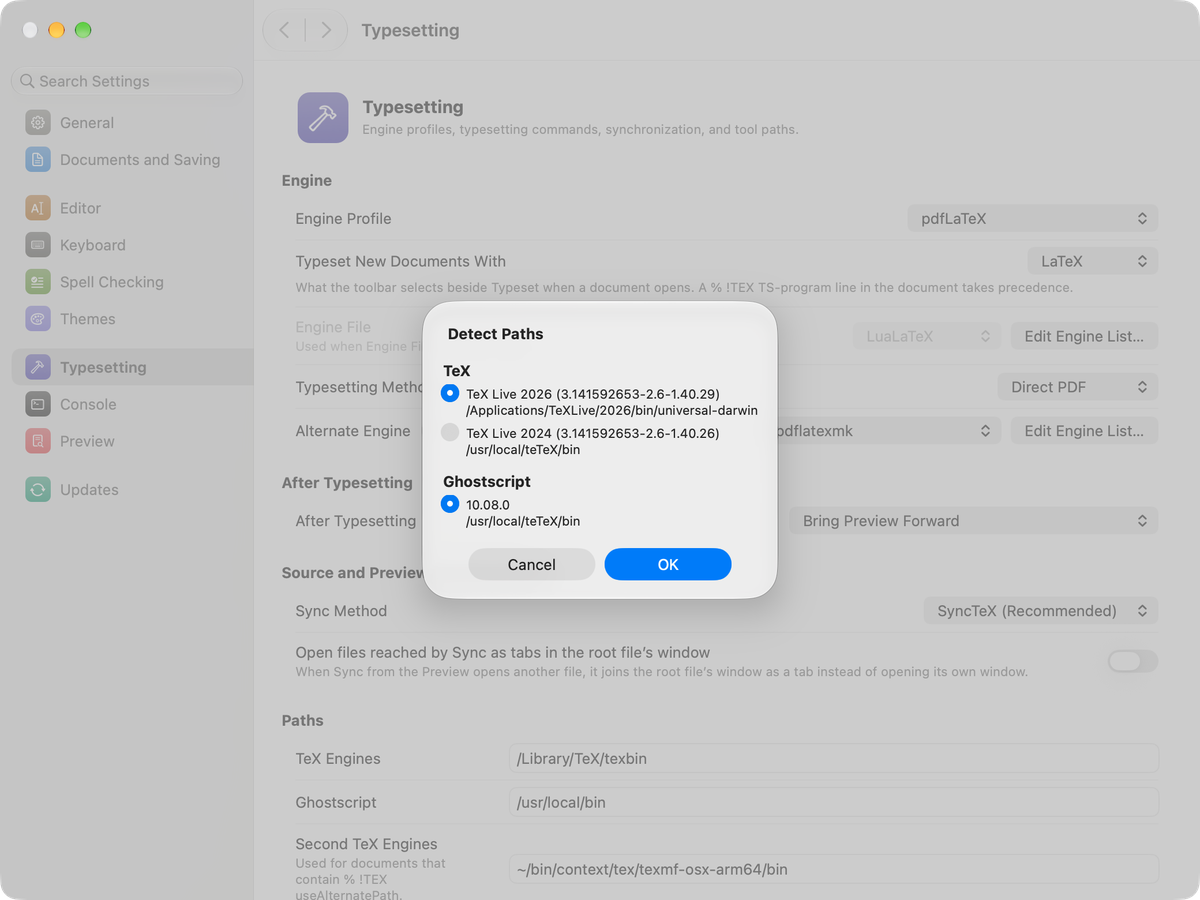
\includegraphics[width=0.8\textwidth]{Graphics/manual-detect-paths.png}
   \caption{Detect Paths\ldots\ with two \TeX\ Live installations and one Ghostscript}
   \label{fig:DetectPaths}
\end{figure}

\mnu{Detect Paths\ldots} (\cref{fig:DetectPaths}) looks for \TeX\ and Ghostscript in the usual places, including the folders of \path{/etc/paths} and \path{/etc/paths.d}, \path{/Library/TeX/texbin}, the \TeX\ Live folders in \path{/usr/local/texlive} and \path{/Applications/TeXLive}, and the folders of Homebrew, MacPorts and Fink. It checks that the programs run, and lists the installations it finds with their versions, newest first. The newest one is selected, but another can be chosen, separately for \TeX\ and for Ghostscript; \mnu{OK} sets the paths. An installation in another place can be entered by hand.

\section{BibTeX}\label{sec:bibtex}

BibTeX builds the bibliography of a \LaTeX\ document from a database of references, a file with the extension \verb|.bib|. The document cites entries by their keys, and BibTeX lists only the entries cited. A database \verb|mybibliography.bib| contains entries such as
\begin{verbatim}
     @book{Knuth:TeXbook,
       author    = {Donald E. Knuth},
       title     = {The {\TeX}book},
       publisher = {Addison-Wesley},
       year      = {1986}
     }
\end{verbatim}
and the document cites them and names the style and the database:
\begin{verbatim}
     As explained in~\cite{Knuth:TeXbook}, ...
     \bibliographystyle{plain}
     \bibliography{mybibliography}
\end{verbatim}

To build the bibliography:
\begin{enumerate}
\item Typeset the document. Citations appear as [?], and the bibliography is missing.
\item Choose \mnu{Typeset}\To\mnu{BibTeX} (\shiftkey-\cmdkey-B), or choose BibTeX in the toolbar and press \mnu{Typeset}.
\item Typeset twice more: the first run adds the bibliography, the second fills in the citations.
\end{enumerate}
Typesetting with latexmk, for instance with the pdflatexmk engine or a profile set up \mnu{With latexmk}, runs BibTeX and the extra passes by itself.

TeXShop can edit the database. When you save a new database from TeXShop, choose the bib file type in the Save dialog, so that the file gets the extension \verb|.bib|.

\mnu{Typeset}\To\mnu{BibTeX} runs the command in \mnu{Settings}\To\mnu{Typesetting}\To\mnu{Related Tools}\To\mnu{BibTeX Engine}, bibtex by default. Enter another program there with any options it needs, for instance biber for documents that use the biblatex package. To choose the program for one document, put a line like this in one of its first twenty lines:
\begin{verbatim}
     % !BIB program = biber
\end{verbatim}
The line takes precedence over the setting. The form \verb|% !BIB TS-program =| is read the same way.

\section{MakeIndex}\label{sec:makeindex}

MakeIndex sorts the index entries of a \LaTeX\ document and writes the index. To add an index to a document, put
\begin{verbatim}
     \usepackage{makeidx}
     \makeindex
\end{verbatim}
in the preamble, put \verb|\printindex| where the index should appear, often just before \verb|\end{document}|, and mark the entries in the text:
\begin{verbatim}
     There are many animals in the world\index{animal}.
     Examples include bears\index{animal!bear}
     and tigers\index{animal!tiger}.
\end{verbatim}
To create the index, typeset the document, choose \mnu{Typeset}\To\mnu{MakeIndex} (\shiftkey-\cmdkey-I), and typeset again. Typesetting with latexmk runs MakeIndex by itself.

MakeIndex runs the program in the \mnu{Index Program} field of the \mnu{Related Tools} group, followed by the name of the idx file. The default is makeindex. Fill in another program, such as mendex or upmendex for Japanese documents, with any options it needs, for instance \verb|upmendex -s mystyle.ist|.

\section{MetaPost}\label{sec:metapost}

\mnu{Typeset}\To\mnu{MetaPost} (\shiftkey-\cmdkey-M) runs MetaPost on the active document, a file with the extension \verb|.mp|. It runs the command in the \mnu{MetaPost} field of the \mnu{Related Tools} group; the default is mpost. The profiles pLaTeX + dvipdfmx and upLaTeX + dvipdfmx set pmpost and upmpost, which typeset Japanese text in labels. Lua\LaTeX\ cannot include figures whose labels pmpost or upmpost typeset in Japanese; with Lua\LaTeX, draw such figures in the document with the luamplib package.

% ===== 07-engines.tex
\chapter{Engines and latexmk}\label{chap:engines}

Besides the built-in plain \TeX\ and \LaTeX, TeXShop typesets with \emph{engines}: small shell scripts with the extension \verb|.engine| in the folder \path{~/Library/TeXShop/Engines}. An engine can run a single program, or a chain of programs, for instance Lua\LaTeX, then Biber, then Lua\LaTeX\ twice more. Any typesetting job that can be written as a script fits this scheme.

\section{Engine Files}\label{sec:engines}

Choose \mnu{TeXShop}\To\mnu{Open \textasciitilde/Library/TeXShop} and open the \mnu{Engines} folder. Each file with the extension \verb|.engine| is an engine, listed under its name without the extension in the pop-up menu beside the \mnu{Typeset} button. TeXShop comes with engines such as LuaLaTeX, XeLaTeX and pdflatexmk; the subfolder \mnu{Inactive} holds many more (\cref{sec:inactive-folder}). An engine file can be opened and edited in TeXShop.

Here is \verb|XeLaTeX.engine|:
\begin{verbatim}
     #!/bin/tcsh

     set path= ($path /Library/TeX/texbin /usr/texbin /usr/local/bin)
     xelatex  -file-line-error -synctex=1 "$1"
\end{verbatim}
The first line names the shell that runs the script. The second adds the usual folders of the \TeX\ programs to the search path. The last line does the work: it typesets the file \verb|"$1"|, the source file, with xelatex and the two options that TeXShop relies on (\cref{sec:direct-pdf-via-dvi}).

\section{Typesetting with an Engine}\label{sec:typesetting-with-engine}

Choose the engine in the pop-up menu beside the \mnu{Typeset} button, and press \mnu{Typeset} or type \cmdkey-T. The choice applies to the document in that window only, so one open document can be typeset with your usual program and another with Xe\LaTeX.

To typeset new documents with an engine, choose \mnu{Engine File} in the \mnu{Typeset New Documents With} pop-up menu of \mnu{Settings}\To\mnu{Typesetting}, and choose the engine in the \mnu{Engine File} menu below it (\cref{sec:choosing-program}).

To tie a document to an engine, put a line like this in one of its first twenty lines:
\begin{verbatim}
     % !TEX program = XeLaTeX
\end{verbatim}
\cmdkey-T then always typesets the document with that engine. The name is the name of the engine file without \verb|.engine|; case does not matter. The names of the built-in programs, such as \verb|pdflatex| and \verb|tex|, are listed in \cref{sec:choosing-program}. The line takes precedence over the toolbar, the settings and \mnu{Typeset with Alternate Engine}. The older form \verb|% !TEX TS-program =| is read the same way. In a project with a root file, only the root file needs the line (\cref{chap:projects}).

Write the line exactly as shown, with one space on each side of the equals sign. The \mnu{Program} macro in the \mnu{Macros} menu writes a program line for you: it lists the built-in programs and the engines, and puts a line in the older form, such as \verb|% !TEX TS-program = xelatex|, at the top of the document for the one you choose. It replaces an earlier \verb|% !TEX TS-program| line, but not a \verb|% !TEX program| line; delete such a line yourself, so that the document has only one program line.

\section{latexmk}\label{sec:latexmk}

Some documents need several runs. \TeX\ writes the table of contents, cross-references and citations into auxiliary files and reads them in the next run, and an index or a bibliography needs a run of MakeIndex or BibTeX between two runs of \TeX. The script latexmk by John Collins, part of \TeX\ Live, runs \LaTeX\ and these programs as many times as needed for an up-to-date document.

TeXShop comes with two engines that typeset with latexmk:
\begin{description}
\item[pdflatexmk] runs latexmk with pdf\LaTeX.
\item[sepdflatexmk] does the same with \verb|--shell-escape| (see \cref{sec:direct-pdf-via-dvi} before using it).
\end{description}
The folder \path{Engines/Inactive/Latexmk} holds latexmk engines for other programs, such as xelatexmk, lualatexmk and dvipdfmxmk, together with documentation. An engine profile set up \mnu{With latexmk} is another way to typeset with latexmk (\cref{sec:configuring-typesetting}).

The latexmk engines accept options for the \TeX\ program from the document, through a line near its top such as
\begin{verbatim}
     % !TEX parameter = -shell-escape
\end{verbatim}
Several options can be given, separated by spaces.

The engines share a set of latexmk settings that make several popular packages work, such as glossaries. They are in \path{~/Library/TeXShop/bin/latexmkrcedit}, which the engines create from \path{~/Library/TeXShop/bin/tslatexmk/latexmkrcDONTedit} the first time they run. Edit \verb|latexmkrcedit| to change the settings for all latexmk engines; TeXShop leaves it alone. For the settings of one project, put a latexmk configuration file named \verb|platexmkrc| in the folder of its root file; the engines read it after their own settings.

\subsection{Typeset with Alternate Engine}

latexmk takes longer than a single run. One way to work is to typeset with a fast program while writing, and with latexmk now and then. \mnu{Typeset}\To\mnu{Typeset with Alternate Engine} (\ctlkey-\optkey-\cmdkey-T) typesets once with the engine chosen in \mnu{Settings}\To\mnu{Typesetting}\To\mnu{Alternate Engine}, pdflatexmk by default, without changing the toolbar. In the \mnu{Typeset} menu, it appears in place of \mnu{Typeset} while you hold down Control and Option. The menu \mnu{Alternate Engine} offers plain \TeX\ and \LaTeX\ with each typesetting method, and the engine files in \path{~/Library/TeXShop/Engines}. To use another latexmk engine, for instance xelatexmk for a document typeset with Xe\LaTeX, move it from the Inactive folder to the Engines folder and choose it there. \mnu{Edit Engine List...} beside the menu opens the Engines folder in the Finder. The info button beside its name tells where \mnu{Typeset with Alternate Engine} is in the \mnu{Typeset} menu and its current key. A \verb|% !TEX program| line in the document takes precedence over the Alternate Engine.

\section{The Inactive Folder}\label{sec:inactive-folder}

The subfolder \mnu{Inactive} of the Engines folder contains engines for special workflows, such as latexmk, ConTeXt, Sage, PreTeXt, pythontex and Typst, often with documentation and sample documents. Engines in this folder are not listed in the toolbar. To use one, move or copy it from its folder to the Engines folder itself.

When TeXShop is updated, it writes the current versions of its files into the Inactive folder, replacing the earlier ones, but it never changes the files directly in the Engines folder. So edit engines only after moving them to the Engines folder.

\section{Writing an Engine}\label{sec:creating-engine}

The easiest way to make an engine is to duplicate one in the Engines folder in the Finder, rename the copy, and open it in TeXShop to edit it. An engine file must have the extension \verb|.engine| and permission to be executed, which a duplicate keeps. Documents opened afterwards list the new engine in their toolbar.

The first line of an engine names its shell or language, for instance
\begin{verbatim}
     #!/bin/zsh
\end{verbatim}
zsh is the default shell of macOS; bash, tcsh, sh, Perl and others work as well, as long as the rest of the script is written in that language. Shells differ in syntax, so a line that works in one may fail in another.

TeXShop runs the engine in the folder of the source file and passes it three values:
\begin{description}
\item[\texttt{\$1}] The name of the source file with its extension, without its folder, such as \verb|Galois.tex|. In a project, this is the root file. A script that changes to another folder must note the full path first, for instance as \verb|"$PWD/$1"|.
\item[\texttt{\$2}] The rest of a line \verb|% !TEX parameter =| near the top of the source (in a project, the root file), with leading and trailing spaces removed; it may contain several flags separated by spaces. Without such a line it is a single space. The form \verb|% !TEX TS-parameter =| is read the same way.
\item[\texttt{\$3}] The folder in \mnu{Settings}\To\mnu{Typesetting}\To\mnu{Paths}\To\mnu{TeX Engines}, or the folder in \mnu{Second TeX Engines} when the source contains the line \verb|% !TEX useAlternatePath|.
\end{description}

Most engines use only \verb|$1|. \verb|$3| serves documents that must be typeset with programs outside the usual \TeX\ installation, such as ConTeXt users who keep the separate ConTeXt distribution: they enter its folder in \mnu{Second TeX Engines} and add \verb|% !TEX useAlternatePath| to their documents, and the engine ConTeXt-CG in the Inactive folder takes its programs from \verb|$3|.

When the engine ends, TeXShop opens the PDF file with the name of the source and the extension \verb|.pdf|, if the engine wrote a new one, in the Preview window. An engine can choose other output with the commands of \cref{sec:engine-commands}.

For example, an engine that runs Lua\LaTeX, Biber and Lua\LaTeX\ twice more could read:
\begin{verbatim}
     #!/bin/zsh
     export PATH="/Library/TeX/texbin:$PATH"
     lualatex --file-line-error --synctex=1 "$1"
     biber "${1:r}"
     lualatex --file-line-error --synctex=1 "$1"
     lualatex --file-line-error --synctex=1 "$1"
\end{verbatim}

\section{Engine Commands}\label{sec:engine-commands}

\subsection{Working with File Names}

An engine often needs the name of the source without its extension, to name other files such as \verb|Galois.pdf| or \verb|Galois.aux|. In zsh:
\begin{verbatim}
     #!/bin/zsh

     filename="$1"
     basename="${filename:r}"
     extension="${filename##*.}"

     echo $filename          # Galois.tex
     echo $basename          # Galois
     echo $extension         # tex
     echo $basename.pdf      # Galois.pdf

     if [[ "$extension" = "ptx" ]]; then
         echo "This is a PreTeXt file"
         exit
     fi
\end{verbatim}
Output of \verb|echo| appears in the console, which helps to test an engine. Shell syntax is strict about spaces: \verb|filename="$1"| fails with spaces around the equals sign, and \verb|[[ ... ]]| needs the spaces after \verb|[[| and before \verb|]]|. These recipes are for zsh and may not work in other shells.

\subsection{Choosing What TeXShop Shows}

The following lines in an engine file tell TeXShop which windows to show when the engine ends. They may be written anywhere in the file, but they must not disturb the script, so write them inside a comment of its language; for a shell script, after \verb|#|:
\begin{verbatim}
     # !TEX-pdfPreview
\end{verbatim}

\begin{center}
\begin{tabular}{ll}
\textbf{Line} & \textbf{Effect}\\ \hline
\verb|!TEX-noPreview| & show no Preview window, whatever other lines are present\\
\verb|!TEX-bothPreview| & show the PDF file and the HTML file\\
\verb|!TEX-pdfPreview| & show the PDF file\\
\verb|!TEX-htmlPreview| & show the HTML file in the HTML window\\
\verb|!TEX-noConsole| & do not show the console\\
\end{tabular}
\end{center}

The first of the four preview lines in this table that the file contains decides; to show both files, use \verb|!TEX-bothPreview|. The PDF and HTML files are those with the name of the source and the extension \verb|.pdf| or \verb|.html|. An engine without any of these lines shows the PDF file, as described in \cref{sec:creating-engine}. \verb|!TEX-noConsole| suits an engine that only opens an HTML file without typesetting, such as the html engine; see \cref{HTMLChapter}.

% ===== 08-projects.tex
\chapter{Projects with Multiple Files}\label{chap:projects}

Large documents are often split into several files: a root file with the preamble includes or inputs a file for each chapter, and the chapter files may sit in folders of their own together with their illustrations. For example, a root file \verb|Main.tex| could read
\begin{verbatim}
     \documentclass[11pt]{book}
     \includeonly{Chapter2/two}
     \begin{document}
     \include{Chapter1/one}
     \include{Chapter2/two}
     \include{Chapter3/three}
     \end{document}
\end{verbatim}
where \verb|\includeonly| lets you typeset only the chapters you are working on.

\section{The Root Line}\label{sec:root-line}

When you edit \verb|two.tex|, TeXShop must typeset \verb|Main.tex|, not the chapter, which has no preamble. To tell it so, put this line in one of the first twenty lines of each chapter file:
\begin{verbatim}
     % !TEX root = ../Main.tex
\end{verbatim}
The root file itself has no such line. The name of the root file can be given
\begin{itemize}
\item by its name alone, \verb|Main.tex|, when it is in the same folder as the chapter file;
\item relative to the folder of the chapter file, as \verb|../Main.tex| or \verb|../../Main.tex|;
\item by its full path, such as \verb|/Users/me/Book/Main.tex|, or by a path that starts with \verb|~| for your home folder. Such a line must be changed when the project moves.
\end{itemize}
Write the line exactly as shown, with one space on each side of the equals sign.

The \mnu{Root} macro in the \mnu{Macros} menu writes the line: it asks for the root file in a file dialog, then offers a relative or an absolute line, and inserts it at the top of the document, replacing an earlier root line.

\section{What the Root Line Does}

\begin{itemize}
\item \mnu{Typeset} in a chapter file typesets the root file, and the Preview window of the root file shows the whole document. Lines that control typesetting, such as \verb|% !TEX program|, \verb|% !TEX parameter| and \verb|% !BIB program|, belong in the root file.
\item \mnu{Goto Error} opens the file that contains an error, if it is not open, and goes to the line (\cref{sec:goto-error}).
\item Synchronization from the Preview window opens the chapter file that contains the clicked spot (\cref{sec:synctex}).
\item \mnu{Trash Aux Files} removes the auxiliary files of the root file (\cref{sec:trash-aux}).
\item \mnu{Window}\To\mnu{Source \(\Leftrightarrow\) Preview} (\cmdkey-1) in a chapter file brings the Preview window of the root file to the front. Pressing it again in the Preview window returns to the source window from which you came.
\item \mnu{Edit}\To\mnu{Find}\To\mnu{Find in TeX Sources with the Same TEX root\ldots} finds and replaces in the root file and in the \verb|.tex| files in its folder and the folders below it that name it in a root line (\cref{TeXRootSearchSection}). In the root file itself the item is \mnu{Find in TeX Sources with This File as TEX root\ldots}.
\end{itemize}

\section{Opening a Chapter File}

When you open a chapter file with a root line, TeXShop also opens the root file and its Preview window, but not the other chapter files. You can then revise the chapter and typeset as usual; the Preview window shows the changes. Two settings in \mnu{Settings}\To\mnu{General}\To\mnu{Project Root File} control this: \mnu{Open the root file when opening a document} turns it on or off, and \mnu{Miniaturize the opened root window} sends the source window of the root file to the Dock, since it is rarely edited while you work on a chapter.

Instead of separate windows, the root file and its chapter files can open as tabs of one window, with the line \verb|% !TEX useTabs| in the root file; see \cref{chap:windows}.

% ===== 09-errors-synctex.tex
\chapter{Errors, Auxiliary Files and SyncTeX}\label{chap:errors-synctex}

\section{Goto Error}\label{sec:goto-error}

When \TeX\ finds an error, it prints a message at the end of the console and waits for an answer, and the console comes to the front. Type the answer in the field at the bottom of the console and press Return; Return alone continues to the next error, and pressing it several times often finishes the run, so that the Preview window shows new output. To stop \TeX, click \mnu{Abort} in the console or choose \mnu{File}\To\mnu{Abort Typesetting} (\ctlkey-\optkey-\cmdkey-A).

\mnu{Edit}\To\mnu{Goto Error} (\ctlkey-\cmdkey-E), also a button in the console, brings the source window forward, scrolls to the line of the first error and highlights it. Choose it again to go to the next error; after the last error it starts again with the first. It is often quickest to fix a few errors and typeset again, since one error can cause several others.

In a project with a root file and chapter files (\cref{chap:projects}), \mnu{Goto Error} opens the file that contains the error, if it is not open, and goes to the line there. To find the file, \mnu{Goto Error} needs the file names that \TeX\ writes with the option \verb|-file-line-error|, which the commands and engines of TeXShop use. Without it, \mnu{Goto Error} goes to the line in the active document. With an external editor, \mnu{Goto Error} goes to the line in that editor; see \cref{ExternalEditorChapter}.

\section{Trash Aux Files}\label{sec:trash-aux}

When \LaTeX\ typesets \verb|Galois.tex|, it writes auxiliary files such as \verb|Galois.aux|, \verb|Galois.toc| and \verb|Galois.log|. The next run reads them for the table of contents, cross-references and the like, so a document may need two or three runs before it is up to date. If typesetting is stopped in the middle, for instance after an error, these files can be left damaged, and the next run reports errors that are not in the source, often just before \verb|\begin{document}|. Moving the auxiliary files to the Trash and typesetting again cures this. The problem is rare for small documents and more common for large documents and documents with many illustrations.

\mnu{File}\To\mnu{Trash Aux Files} (\ctlkey-\cmdkey-A), also a button in the console, moves the auxiliary files of the document to the Trash. \mnu{Typeset}\To\mnu{Trash Aux \& Typeset} (\optkey-\cmdkey-T) does this and then typesets; in the \mnu{Typeset} menu, it appears in place of \mnu{Typeset} while you hold down Option.

The files trashed are those in the folder of the source that have its name and one of these extensions:
\begin{verbatim}
     4ct  4tc  aux  bcf  blg  brf  css  ent  fdb_latexmk  fff  fls
     gaux  glo  glog  gtex  idv  idx  ilg  ind  lg  loa  lof  log
     lot  mlf  mtc  out  pdfsync  run.xml  synctex  synctex.gz  toc
     ttt  wrm  xref
\end{verbatim}
Files that SyncTeX leaves with \verb|(busy)| at the end of their name when typesetting is interrupted, such as \verb|Galois.synctex.gz(busy)|, are trashed as well. The \verb|.bbl| file of BibTeX is kept. On a disk or cloud folder that has no Trash, the files are deleted.

In a project whose chapter files name a root file with \verb|% !TEX root|, the files of the root file are trashed, also when the command is given in a chapter file.

\subsection{Variations}

The following keys change what \mnu{Trash Aux Files} and the button of the console remove. \mnu{Trash Aux \& Typeset} always trashes the auxiliary files of the document alone.
\begin{description}
\item[Shift] Hold down Shift while choosing \mnu{Trash Aux Files} or clicking the button to trash the PDF file of the document as well. Usually the old PDF file is kept, so that the Preview window has something to show when typesetting fails.
\item[Option] Hold down Option while choosing \mnu{Trash Aux Files} or clicking the button to clean up a whole project: every file with one of the extensions above in the folder of the root file and in all folders below it is trashed, whatever its name. This also removes the \verb|.aux| files that \verb|\include| writes for chapters in subfolders. Hidden files and folders are left alone.
\end{description}

Two hidden settings change this behavior. To add extensions to the list, for instance \verb|dvi|, type in Terminal
\begin{verbatim}
     defaults write TeXShop OtherTrashExtensions -array-add "dvi"
\end{verbatim}
and to return to the standard list
\begin{verbatim}
     defaults write TeXShop OtherTrashExtensions -array
\end{verbatim}
To make the Option behavior the standard behavior of \mnu{Trash Aux Files} and \mnu{Trash Aux \& Typeset}:
\begin{verbatim}
     defaults write TeXShop AggressiveTrashAUX YES
\end{verbatim}
See \cref{chap:hidden-settings} for hidden settings in general.

\section{SyncTeX}\label{sec:synctex}

SyncTeX takes you from a place in the source to the corresponding place in the typeset output, and back:
\begin{itemize}
\item Command-click a word in the source window. The Preview window scrolls to the corresponding place and marks it.
\item Command-click a place in the Preview window. The source window comes forward with the corresponding text marked; if the place belongs to another file of the project, that file opens.
\end{itemize}
\mnu{Sync} at the top of the contextual menu of the source and of the Preview window does the same for the place you clicked. The colors of the two marks are set in \mnu{Settings}\To\mnu{Themes}\To\mnu{SyncTeX}, under \mnu{Preview} and \mnu{Source}.

SyncTeX is a part of the \TeX\ engines by J\'er\^ome Laurens. When \TeX\ is run with the option \verb|-synctex=1|, it writes a file such as \verb|Galois.synctex.gz| beside the PDF file, which records where each piece of the source ended up on the page; TeXShop reads it with Laurens's parser. The commands of \mnu{Settings}\To\mnu{Typesetting}, as the engine profiles set them, and the engines that TeXShop puts in \path{~/Library/TeXShop/Engines} and that run \TeX\ use this option. An engine you add there, including one of the optional engines from the Inactive folder, uses it only if its command has it. In an engine of your own, add \verb|-synctex=1| to the call of \TeX\ (with one or two hyphens; every engine accepts both).

SyncTeX is very useful, but not exact: the place you are looking for may be a little before or after the mark.

The synctex file contains the full paths of the source files. After a project folder is moved, copied or sent to someone else, synchronization does nothing until the document is typeset again.

\subsection{Projects with Several Files}

In a project whose chapter files name the root file with \verb|% !TEX root| (\cref{chap:projects}), Command-click in a chapter file goes to its place in the Preview window of the whole document, and Command-click in the Preview window opens the chapter file that contains the clicked spot, if it is not open, and goes to the place there. This is also a quick way to open the chapter you want: open the root file, scroll the Preview window to the place, and Command-click.

With ``Open files reached by Sync as tabs in the root file's window'' on, in the \mnu{Source and Preview Synchronization} group of \mnu{Settings}\To\mnu{Typesetting}, a file that synchronization opens joins the window of the root file as a tab instead of opening its own window.

\subsection{Sync Method}

\mnu{Settings}\To\mnu{Typesetting}\To\mnu{Sync Method} has two choices:
\begin{description}
\item[SyncTeX (Recommended)] uses the synctex file, as described above. This is the default.
\item[Search PDF] searches the PDF file for the text around the click, and the source for the text around a click in the Preview window. It needs no synctex file, but it fails where the typeset text differs from the source, as in formulas and text with many commands. To find the file of a spot in the Preview window, it searches the files named in the \verb|\include| and \verb|\input| commands of the root file; for projects that include files in another way, list them in the root file with \verb|% !TEX projectfile| lines (\cref{chap:magic-comments}).
\end{description}

ConTeXt has synchronization code of its own, which TeXShop uses with the line \verb|% !TEX useConTeXtSyncParser|; see \cref{ConTeXtChapter}. To synchronize with a source open in another editor, see \cref{ExternalEditorChapter}.

\section{Page Numbers in the Page Number Box}\label{sec:page-number-box}

The page number box in the toolbar of the Preview window shows the number of the current page, and typing a number there and pressing Return goes to that page. Normally these are page numbers counted from the first page of the PDF file. In a book with front matter, such as a title page, a preface and a table of contents numbered i, ii, iii, \dots, followed by the main text numbered 1, 2, 3, \dots, these numbers differ from the numbers printed on the pages.

TeXShop can bring them into line. It then numbers the front matter pages \verb|1#|, \verb|2#|, \verb|3#|, \dots, and the main pages 1, 2, 3, \dots, the numbers printed on them. Typing a plain number such as \verb|12| goes to page 12 of the main text, and typing \verb|3#| goes to the third page of the front matter. The box with the total number of pages still shows the number of all pages.

TeXShop does this when \TeX\ writes a line such as
\begin{verbatim}
     Start of main material: 17.
\end{verbatim}
to the console and the log file, where 17 is the physical page, counted from the first page of the PDF file, on which the main material begins. TeXShop looks for this line while the document is typeset, and in the log file when a document is opened.

In a \LaTeX\ document, put the following line at the place where the main material begins:
\begin{verbatim}
     \write128{Start of main material: \the\ReadonlyShipoutCounter.}
\end{verbatim}
In the book class and other classes with the command \verb|\mainmatter|, you can instead add these lines to the preamble, so that \verb|\mainmatter| writes the line:
\begin{verbatim}
     \let\OLDmain=\mainmatter
     \renewcommand{\mainmatter}{\OLDmain
       \write128{Start of main material: \the\ReadonlyShipoutCounter.}}
\end{verbatim}

Plain \TeX\ has no counter of the pages written so far. If the main material of a plain \TeX\ document begins on, say, physical page 5, write the number yourself:
\begin{verbatim}
     \message{Start of main material: 5.}
\end{verbatim}

To have these lines at hand, add them to a template, a macro or the command completion list.

The same works for a PDF file opened in TeXShop without its source. If a log file with the same name is next to the PDF file, TeXShop reads it when it opens the PDF file. You can also write such a file yourself: for a manual \verb|Manual.pdf| with two pages of front matter, a plain text file \verb|Manual.log| next to it containing
\begin{verbatim}
     Start of main material: 3.
\end{verbatim}
makes TeXShop number the pages accordingly.

A \verb|% !TEX numberingCorrection| line in a document turns this automatic numbering off and sets the numbering by hand instead; see \cref{chap:magic-comments}.

% ===== 10-encodings.tex
\chapter{Encodings}\label{EncodingsChapter}

\section{About Encodings}

TeXShop edits text in Unicode, so a source window can hold English, Cyrillic, Chinese, Hebrew and Arabic in one document. A file on disk, however, is a stream of bytes, and an {\em encoding} decides how characters are written as bytes and read back.

UTF-8 can store every Unicode character, and plain ASCII text is already valid UTF-8. \LaTeX\ reads UTF-8 by default, and XeLaTeX and LuaLaTeX expect it. New users should use UTF-8 and need read no further.

Older files, and files from other people, may use another encoding, such as ISO Latin 9 for Western Europe or Shift JIS for Japanese. Most of these encodings store one character per byte and give the bytes from 128 to 255 a different meaning in each encoding. Such a file does not say which encoding it uses, and reading it in the wrong one turns some characters into others. A document is saved in the encoding it was read in, so an older file keeps its encoding; characters that this encoding cannot represent are lost when the file is saved.

\section{New Documents}

New documents are saved in \mnu{Encoding for new documents}, in the Encoding group of the Documents and Saving category of TeXShop Settings. It is \mnu{Unicode (UTF-8)} by default. Changing it does not change documents that are already open.

\section{Opening Files}\label{sec:EncodingDetection}

When a file without an encoding line (\cref{sec:EncodingLine}) is opened, TeXShop detects its encoding:
\begin{itemize}
\item a byte order mark identifies UTF-8 and UTF-16 files;
\item a file of ASCII characters only is read in the encoding for new documents, or in UTF-8 if that encoding does not write ASCII characters as ASCII, as UTF-16 does;
\item otherwise TeXShop uses the encoding that the program which saved the file recorded with it, when macOS has kept this information and the file can be read in it;
\item then it tries UTF-8, which is almost never valid by chance;
\item then it chooses among the encoding for new documents and the encodings of your languages, such as the Japanese, Chinese, Korean, Cyrillic and Western European ones.
\end{itemize}
An encoding that the source declares, for instance with
\begin{verbatim}
     \usepackage[latin1]{inputenc}
\end{verbatim}
is used as a hint. Detection is a guess and works best for files that contain a fair amount of text. It can be turned off with the hidden setting
\begin{verbatim}
     defaults write TeXShop EncodingAutoDetection NO
\end{verbatim}
Files without an encoding line are then read in the encoding for new documents.

{\bf The Open dialog} If detection chooses the wrong encoding, close the file without saving it and open it again with \mnu{File}\To\mnu{Open\ldots}. Click \mnu{Options} in the Open dialog to show its encoding menu, and choose the encoding; it applies to the files you open from the dialog. Left at the encoding for new documents, the menu lets TeXShop detect the encoding of each file. Then add an encoding line to the file, so that it always opens correctly.

{\bf Line endings} Files written on Windows end lines with a carriage return and a line feed (CRLF), and files from very old Macintosh systems with a carriage return (CR). When TeXShop opens such a file, or a file that mixes line endings, it changes all line endings to line feeds (LF), the line endings of macOS, and a notice tells you so, since the file will be saved with LF line endings. Check \mnu{Don’t show again for this document} in the notice to stop it for that file. Line endings in text you paste are changed to LF as well. The hidden setting \texttt{ConvertLF} turns both conversions off (\cref{chap:hidden-settings}).

{\bf Commands of the otf package} The \verb|\UTF{...}| and \verb|\CID{...}| commands that the \texttt{otf} package uses for characters outside JIS~X~0208 are shown as the characters themselves when a file is opened; see \cref{JapanChapter}.

\section{The Encoding Line}\label{sec:EncodingLine}

A magic comment line among the first 20 lines of a source file fixes the encoding of that file, for reading and for saving, overriding everything else:
\begin{verbatim}
% !TEX encoding = UTF-8 Unicode
\end{verbatim}
Write the line exactly in this form: \verb|% !TEX|, one space on each side of the equals sign, and the name of the encoding exactly as in the left column of \cref{tab:Encodings}, including capitalization. The easy way is \mnu{Macros}\To\mnu{Encoding}: it lists the encodings and writes the line at the top of the source, replacing an earlier one. The names that TeXworks uses, such as \texttt{UTF-8}, \texttt{ISO 8859-1} or \texttt{Shift-JIS}, are also understood.

If the line names an encoding that TeXShop does not know, TeXShop says so and reads the file as UTF-8. If the line names UTF-8 but the file is not valid UTF-8, TeXShop reports it and opens the file in ISO Latin 9, which can read any file; saving it without changing the line writes the same bytes back, so nothing is lost. To open a file without applying its encoding line, hold down \optkey\ while it opens.

\begin{table}[htbp]
\centering
\begin{tabular}{ll}
\hline
Name in the encoding line & Name in the menus \\
\hline
\texttt{MacOSRoman} & Western (Mac OS Roman) \\
\texttt{IsoLatin} & Western (ISO Latin 1) \\
\texttt{IsoLatin2} & Central European (ISO Latin 2) \\
\texttt{IsoLatin5} & Turkish (ISO Latin 5) \\
\texttt{IsoLatin9} & Western (ISO Latin 9) \\
\texttt{IsoLatinGreek} & Greek (ISO 8859-7) \\
\texttt{Mac Central European Roman} & Mac Central European Roman \\
\texttt{MacJapanese} & Japanese (Mac OS, ShiftJIS ¥) \\
\texttt{DOSJapanese} & Japanese (Windows, DOS, ShiftJIS \textbackslash) \\
\texttt{SJIS\_X0213} & Japanese (Shift JIS X0213) \\
\texttt{EUC\_JP} & Japanese (EUC) \\
\texttt{JISJapanese} & Japanese (ISO 2022-JP) \\
\texttt{MacKorean} & Korean (Mac OS) \\
\texttt{DOSKorean} & Korean (Windows, DOS) \\
\texttt{UTF-8 Unicode} & Unicode (UTF-8) \\
\texttt{Standard Unicode} & Unicode (UTF-16) \\
\texttt{Mac Cyrillic} & Cyrillic (Mac OS) \\
\texttt{DOS Cyrillic} & Cyrillic (DOS) \\
\texttt{DOS Russian} & Russian (DOS) \\
\texttt{Windows Latin 1} & Windows Latin 1 \\
\texttt{WindowsCentralEurRoman} & Central European Roman (Windows) \\
\texttt{Windows Cyrillic} & Cyrillic (Windows) \\
\texttt{KOI8\_R} & Russian (KOI8-R) \\
\texttt{Mac Chinese Traditional} & Traditional Chinese (Mac OS) \\
\texttt{Mac Chinese Simplified} & Simplified Chinese (Mac OS) \\
\texttt{DOS Chinese Traditional} & Traditional Chinese (Windows, DOS) \\
\texttt{DOS Chinese Simplified} & Simplified Chinese (Windows, DOS) \\
\texttt{GBK} & Chinese (GBK) \\
\texttt{GB 2312} & Simplified Chinese (GB 2312) \\
\texttt{GB 18030} & Chinese (GB 18030) \\
\texttt{Ascii} & Ascii \\
\hline
\end{tabular}
\caption{The encodings of TeXShop, in the order of its encoding menus}
\label{tab:Encodings}
\end{table}

\section{Saving in Another Encoding}

A document is saved in the encoding it was opened with. There are two ways to choose another encoding:
\begin{itemize}
\item turn on \mnu{Show Encoding in Save Dialog} in the Documents and Saving category of Settings; the Save dialog then has an encoding menu, and the encoding chosen there is used for that save and from then on;
\item \mnu{Edit}\To\mnu{Transformations}\To\mnu{Change Encoding} chooses the encoding in which the open document is saved from then on.
\end{itemize}
If the file has an encoding line naming an encoding that TeXShop knows, the line decides, and the menu in the Save dialog shows that encoding and cannot be changed; edit the line instead.

TeXShop keeps the byte order mark of a UTF-8 file and the byte order of a UTF-16 file when it saves the file. Encoding lines are also recognized in UTF-16 files.

\section{Converting Files}

Converting a file to another encoding is risky; keep a copy of the original first. When TeXShop reads a file, it converts every character to Unicode; when it saves the file in another encoding, characters that the new encoding cannot represent are lost. Reading a file in the wrong encoding is worse: the bytes are taken for other characters, and saving the file makes the mistake permanent, even if the new encoding could have represented the original characters.

The command line program \texttt{iconv} converts a file into a new file and leaves the original as it was; use it when you must convert. The document \mnu{File Encoding and TeXShop} in the Help menu discusses these questions in more detail.

If you have a mixture of UTF-8 and older ISO Latin 9 files, keep UTF-8 as the encoding for new documents: detection opens the older files correctly in almost all cases. Once you know that a file is in ISO Latin 9, add the line
\begin{verbatim}
% !TEX encoding = IsoLatin9
\end{verbatim}
so that it always opens in that encoding. Since \LaTeX\ expects UTF-8, such a document also needs these lines in its preamble:
\begin{verbatim}
     \usepackage[T1]{fontenc}
     \usepackage[latin9]{inputenc}
\end{verbatim}

\section{Right-to-Left Languages}\label{sec:RightToLeft}

Arabic, Hebrew and Persian are written from right to left, and the source window enters them that way. A source file often mixes \LaTeX\ commands, written from left to right, with text in these languages. When \mnu{Right-to-left languages (Arabic, Hebrew, Persian)} is on, in the Typing group of the Editor category of Settings, and syntax highlighting is on, a line with a Hebrew or Arabic letter among its first three characters is aligned to the right, and other lines, for instance those that begin with a \LaTeX\ command, to the left. With the hidden setting
\begin{verbatim}
     defaults write TeXShop RightJustifyIfAny YES
\end{verbatim}
every line that contains such a letter anywhere is aligned to the right.

The alignment is only for editing; \TeX\ lays out the typeset text according to its own commands. To typeset these languages, use XeLaTeX or LuaLaTeX. Choose a source font that contains the letters of the language (\cref{Font_Size}). To type them, add an input source for the language in \mnu{System Settings}\To\mnu{Keyboard}, under Text Input, and switch input sources with the input menu in the menu bar. \mnu{Edit}\To\mnu{Character Info\ldots} shows the Unicode name and code point of the selected characters.

% ===== 11-magic-comments.tex
\chapter{Magic Comment Lines}\label{MagicCommentsChapter}\label{chap:magic-comments}

A magic comment line is a \TeX\ comment that TeXShop reads to set something for one document: the typesetting program, the encoding, the root file of a project, and more. \TeX\ ignores these lines.

\section{Writing Magic Lines}

\begin{itemize}
\item A magic line must be among the first 20 lines of the source file. The exceptions are \verb|% !TEX projectfile| and \verb|% !TEX tabbedFile|, described below.
\item Write the line exactly as shown in this chapter, at the beginning of a line. Capitalization matters, and so do the spaces: one after \verb|%|, and one on each side of an equals sign. The lines for program, parameter, encoding, root, spellcheck and projectfile, and \verb|% !BIB program|, are also accepted without the space after \verb|%|, as in \verb|%!TEX root =|.
\item The \mnu{Macros} menu writes the most common lines for you: \mnu{Program} lists the built-in programs and the engines, \mnu{Encoding} the encodings, and \mnu{Root} asks for the root file; each writes its line at the top of the source, replacing an earlier one. \mnu{Program} writes the older form \verb|% !TEX TS-program =| and replaces only a line of that form, so delete a \verb|% !TEX program| line yourself. Further lines are in \mnu{Macros}\To\mnu{Special Comments}.
\end{itemize}

The lines that set the program, its parameter, the BibTeX program and the root file are read each time the document is typeset. The encoding line is read when the document is opened and when it is saved. The other lines are read when the document is opened; after changing one of them, close the document and open it again. \verb|% !TEX numberingCorrection| is also read at each typesetting and by \mnu{Source}\To\mnu{Rescan Magic Comments}.

\section{Typesetting}

\begin{description}
\item[\texttt{\% !TEX program = }{\em name}] Sets the program that typesets this file, overriding the choice in the toolbar and in Settings; \mnu{Typeset}\To\mnu{plain TeX} and \mnu{Typeset}\To\mnu{LaTeX} ignore it. Upper and lower case do not matter in the name. \texttt{pdflatex} and \texttt{pdftex} run the \LaTeX\ and plain \TeX\ commands of the Direct PDF group of the Typesetting category of Settings; \texttt{latex} and \texttt{tex} run those of the Via DVI group; \texttt{personallatex} and \texttt{personaltex} those of the Personal Script group. Any other name is the name of an engine as it appears in the menu beside the Typeset button, such as \texttt{xelatex}, \texttt{lualatex} or \texttt{pdflatexmk}. The older form \verb|% !TEX TS-program =|, which \mnu{Macros}\To\mnu{Program} writes, is also accepted. For example:
\begin{verbatim}
% !TEX program = lualatex
\end{verbatim}
\item[\texttt{\% !TEX parameter = }{\em text}] Passes {\em text} to an engine file as its second argument, \verb|$2|; without this line, the second argument is a single space. An engine can use it to do one of several tasks. The older form \verb|% !TEX TS-parameter =| is also accepted.
\item[\texttt{\% !BIB program = }{\em name}] Runs {\em name} instead of the BibTeX Engine of Settings when \mnu{Typeset}\To\mnu{BibTeX} is chosen, for instance \texttt{biber}. The program must be in the folder of the TeX programs. The older form \verb|% !BIB TS-program =| is also accepted.
\item[\texttt{\% !TEX root = }{\em file}] Names the root file of a project, as a full path or a path relative to this file. Put it at the top of each chapter file that the root file includes, never in the root file itself. Typesetting a chapter file then typesets the root file. See \cref{chap:projects}.
\item[\texttt{\% !TEX useAlternatePath}] Runs the programs of this document from the folder \mnu{Second TeX Engines} in the Paths group of the Typesetting category of Settings, instead of TeX Engines. It is mainly for a separate ConTeXt distribution; see \cref{ConTeXtGardenSection}.
\end{description}

\section{Encoding and Spelling}

\begin{description}
\item[\texttt{\% !TEX encoding = }{\em name}] Fixes the encoding in which this file is read and saved, overriding every other way of choosing it, for instance \verb|% !TEX encoding = UTF-8 Unicode|. The names are listed in \cref{tab:Encodings}; see \cref{sec:EncodingLine}.
\item[\texttt{\% !TEX spellcheck = }{\em language}] Opens this document with the given spelling dictionary instead of the default one, for instance \verb|% !TEX spellcheck = de-DE| for German. The Spelling and Grammar panel can still switch dictionaries while you work. See \cref{SpellCheckingDictionaries}.
\end{description}

\section{Preview}

\begin{description}
\item[\texttt{\% !TEX pdfSinglePage}] Opens the Preview window of this document in Single Page display format, whatever page style is chosen in the Preview category of Settings. Slides, made with Beamer or another slide package, are best seen one page per screen and paged through slide by slide, while articles and books are easier to read in the Multi-Page style.
\item[\texttt{\% !TEX bookDisplay}] In the two-page styles, the first page stands alone, as the cover, and the pairs of pages after it are those of an open book.
\item[\texttt{\% !TEX standardDisplay}] In the two-page styles, the pairs begin with the first page.
\item[\texttt{\% !TEX PageDirectionL2R}] In the two-page styles, pages run from left to right, as for languages written from left to right.
\item[\texttt{\% !TEX PageDirectionR2L}] In the two-page styles, pages run from right to left, as for vertical Japanese text and languages written from right to left.
\end{description}
The last four lines override \mnu{Show first page alone as cover} and \mnu{Page direction} in the Preview category of Settings for this document.

\begin{description}
\item[\texttt{\% !TEX numberingCorrection = }{\em n} \texttt{+ current - desired}] Makes the page number box of the toolbar show the page numbers printed in the document, when automatic correction does not work for it. Replace {\em n} by the number of pages before page~1; only the number counts, and the rest of the line is a reminder. If the box later shows page 78 where the document shows 72, the new number is {\em n} + 78 $-$ 72. \mnu{Macros}\To\mnu{Numbering} inserts the line. See \cref{sec:page-number-box}.
\end{description}

\section{Synchronization}

\begin{description}
\item[\texttt{\% !TEX useConTeXtSyncParser}] Synchronizes this document with the SyncTeX parser of ConTeXt instead of the one built into TeXShop. Recommended for ConTeXt documents; see \cref{ConTeXtSyncSection}.
\item[\texttt{\% !TEX useOldSyncParser}] Synchronizes this document with an older version of the SyncTeX parser that TeXShop also contains, for SyncTeX files that the current parser cannot read. \verb|% !TEX useConTeXtSyncParser| takes precedence over it.
\item[\texttt{\% !TEX projectfile = }{\em file}] Used only when the Sync Method in the Typesetting category of Settings is Search PDF. To find the source of a spot in the Preview window, TeXShop then searches the files named in the \verb|\include| and \verb|\input| commands of the root file; ConTeXt includes files differently, so list the files of such a project in the root file with these lines, one file per line. A name is a full path or a path relative to the root file. These lines may appear anywhere in the root file.
\end{description}

\section{Tabs}

These lines in a root file open the files of the project as tabs of its source window; see \cref{ProjectTabsSection} for details and examples. A root file with one of them opens in separate source and Preview windows, even when \mnu{Source and Preview} is set to \mnu{Use One Window}.

\begin{description}
\item[\texttt{\% !TEX useTabs}] Opens the files of the \verb|\include| commands of the root file as tabs, up to 20 files. Short names for the tabs may follow in parentheses, separated by commas, as in \verb|% !TEX useTabs (Intro, Theory, Examples)|. With the hidden setting \texttt{TabsAlsoForInputFiles}, the files of \verb|\input| commands are opened too.
\item[\texttt{\% !TEX useTabsWithFiles}] Opens the files named by \verb|% !TEX tabbedFile| lines as tabs instead.
\item[\texttt{\% !TEX tabbedFile\{}{\em path}\texttt{\}(}{\em short name}\texttt{)}] Names one file to open as a tab, with a full path or a path relative to the root file; the short name in parentheses is optional. These lines must be among the first 50 lines.
\end{description}

\section{Pseudo-Magic Lines for Engine Files}\label{sec:EnginePseudoMagicLines}

The following lines go in engine files in \texttt{\textasciitilde/Library/TeXShop/Engines}, not in source files. They may appear anywhere in the engine file and anywhere on a line. Since engine files can be written in many languages, the lines do not begin with a comment character; put them inside a comment of the engine's language, so that the engine itself does not see them.
\begin{verbatim}
     !TEX-noPreview
     !TEX-pdfPreview
     !TEX-htmlPreview
     !TEX-bothPreview
     !TEX-noConsole
\end{verbatim}
Without any of these lines, TeXShop opens the PDF file with the name of the source in the Preview window after the engine finishes. Otherwise:
\begin{itemize}
\item with \texttt{!TEX-noPreview}, no preview appears, whatever other lines are present;
\item with \texttt{!TEX-pdfPreview} or \texttt{!TEX-bothPreview}, TeXShop opens the PDF file with the name of the source in the Preview window;
\item with \texttt{!TEX-bothPreview}, or with \texttt{!TEX-htmlPreview} and no \texttt{!TEX-pdfPreview}, TeXShop opens the HTML file with the name of the source in the HTML window;
\item with \texttt{!TEX-noConsole}, the console is not shown; this is meant for engines that open HTML directly, without typesetting.
\end{itemize}
See \cref{chap:engines,HTMLChapter}.

% ===== 12-editing.tex
\chapter{The Source Editor}\label{EditingChapter}

The source window is a full text editor with many aids for writing \TeX. All of them are optional: use the ones that suit the way you type and ignore the others. This chapter describes the editing commands, the ways to move around the source, key bindings, command completion and marks, label and citation key completion, the commands that work with the clipboard or convert characters, and the status bar with its text statistics. Finding and replacing is described in \cref{FindChapter}, macros in \cref{MacrosChapter}, and keyboard shortcuts in \cref{KeyboardChapter}.

\section{Editing Commands}\label{EditingCommandsSection}

\begin{description}
\item[Comment and Uncomment] \mnu{Source}\To\mnu{Comment} (\cmdkey-\{) puts \verb|%| at the start of each selected line, and \mnu{Source}\To\mnu{Uncomment} (\cmdkey-\}) removes it. \mnu{Edit}\To\mnu{Paste As Comment} pastes the text on the clipboard above the current line, with each of its lines commented out.
\item[Indent and Unindent] \mnu{Source}\To\mnu{Indent} and \mnu{Source}\To\mnu{Unindent} move the selected lines right or left: by a tab when \mnu{Use Tabs for Indent Menu} is on in the \mnu{Style} group of the \mnu{Editor} category of TeXShop Settings, and otherwise by as many spaces as \mnu{Tab Size}.
\item[Selecting between brackets] Double-click a bracket, such as \verb|(| or \verb|}|, to select everything from it to its matching bracket; this helps to find a brace that is missing. Double-click with the Option key held down to select the bracket alone. How matching brackets are shown while you type is set in the \mnu{Matching Brackets} group of the \mnu{Editor} category of Settings.
\item[Selecting an environment] Double-click \verb|\begin| or \verb|\end| with the Option key held down to select the whole environment, from \verb|\begin{name}| to the matching \verb|\end{name}|.
\item[Selecting lines] Click a line number to select that line, or drag over the line numbers to select several whole lines; Shift-click a line number to extend the selection to that line. The numbers of the lines selected this way are shown in bold. \mnu{Source}\To\mnu{Show Line Numbers} (\ctlkey-\cmdkey-L) shows or hides the line numbers.
\item[Going to a line] \mnu{Edit}\To\mnu{Line Number\ldots} (\cmdkey-L) asks for a line number and goes to that line.
\item[Closing an environment] \mnu{Source}\To\mnu{Close Current Environment} (\ctlkey-\cmdkey-C) adds the \verb|\end| line of the environment that is still open. For example, after
\begin{verbatim}
   \begin{itemize}
   \item one
   \item two
\end{verbatim}
it adds \verb|\end{itemize}|.
\item[Closing a tag] In HTML and XML files, \mnu{Source}\To\mnu{Close Tag} (\optkey-\cmdkey-.) adds the closing tag of the element that is still open: after \verb|<start>| and \verb|<bf> This is nice </bf>| it adds \verb|</start>|.
\item[XML files] Files with the extension \texttt{xml}, \texttt{html} or \texttt{ptx} are highlighted as XML rather than as \TeX, and command completion uses a list of its own for them. \mnu{Source}\To\mnu{Toggle XML} switches the document in front between the two kinds of highlighting, whatever its extension.
\end{description}

\subsection{Dropping Files on the Source}\label{DragAndDropSection}

Drag a file from the Finder onto the source to insert a command for it:

\begin{center}
\begin{tabular}{ll}
\textbf{File} & \textbf{Inserted command} \\ \hline
\texttt{.pdf}, \texttt{.png}, \texttt{.jpg}, \texttt{.jpeg}, \texttt{.tif}, \texttt{.tiff}, \texttt{.eps}, \texttt{.ps} & \verb|\includegraphics[]{path}| \\
\texttt{.bib} & \verb|\bibliography{name}| \\
\texttt{.bst} & \verb|\bibliographystyle{name}| \\
\texttt{.sty} & \verb|\usepackage{name}| \\
\texttt{.cls} & \verb|\documentclass{name}| \\
other files, such as \texttt{.tex} & \verb|\input{path}| \\
\end{tabular}
\end{center}

Here \emph{path} is the path of the file from the folder of the source file, and \emph{name} is the file name without its extension. A file whose path contains a space is not inserted; TeXShop shows a warning instead. To insert something else for a kind of file, add a submenu named \mnu{Drag \& Drop} to the Macros menu; see \cref{DragAndDropMacros}.

\section{Moving with Emacs Keys}\label{EmacsKeysSection}

The text editor of macOS, which TeXShop uses, understands many keystrokes of the editor \textbf{emacs}, so the insertion point can be moved without taking the hands off the keyboard. For example, \ctlkey-F moves the insertion point forward one character and \ctlkey-B back one character; \ctlkey-A and \ctlkey-E go to the start and the end of the line, \ctlkey-N and \ctlkey-P to the next and the previous line, and \ctlkey-K deletes to the end of the line. These keys work in TeXShop as in other Mac applications.

These keystrokes can be changed, and new ones added, with a file named \texttt{DefaultKeyBinding.dict} in \path{~/Library/KeyBindings}. It has nothing to do with the key bindings of TeXShop described in the next section. The file is a list of keystrokes, each with the name of an editing command of macOS; for example
\begin{verbatim}
     "^f" = "moveForward:";
\end{verbatim}
where \verb|^f| stands for \ctlkey-F. The file applies to every application that uses the macOS text editor, and is read when an application starts.

TeXShop adds four commands that can be used in this file: \texttt{moveForwardTo\$:} and \texttt{moveForwardTo\$\$:} move the insertion point to just after the next \verb|$| or \verb|$$|, and \texttt{moveBackwardTo\$:} and \texttt{moveBackwardTo\$\$:} to just before the previous one. Other applications ignore these names. For instance, with the following file, Option-F and Option-B move to the next or previous \verb|$|, and \ctlkey-F and \ctlkey-B to the next or previous \verb|$$|:
\begin{verbatim}
     /* ~/Library/KeyBindings/DefaultKeyBinding.dict */
     {
         "~f" = "moveForwardTo$:";
         "~b" = "moveBackwardTo$:";
         "^f" = "moveForwardTo$$:";
         "^b" = "moveBackwardTo$$:";
     }
\end{verbatim}
This sample only shows the idea: it takes these keys away from their usual commands. Choose keystrokes that you do not otherwise need.

\section{Key Bindings}\label{KeyBindingsSection}

Key bindings make a typed character insert other text. With the list that comes with TeXShop, typing \verb|^| gives \verb|^{}| with the insertion point between the braces, typing \verb|"| gives the \TeX\ quotes \verb|``''| around the insertion point, and typing \"a gives \verb|\"a|. A key binding can also put the selected text inside: select a word and type \verb|^| to get \verb|^{word}|.

Key bindings are off at first. Turn on \mnu{Use key bindings (default for new documents)} in the \mnu{Keyboard} category of TeXShop Settings to have them on in every document you open. \mnu{Source}\To\mnu{Key Bindings} turns them on or off for the document in front, for example to type a character that has a key binding as itself; the \mnu{KeyBindings} item, which can be added to the toolbar, does the same.

\begin{figure}[htbp]
\centering
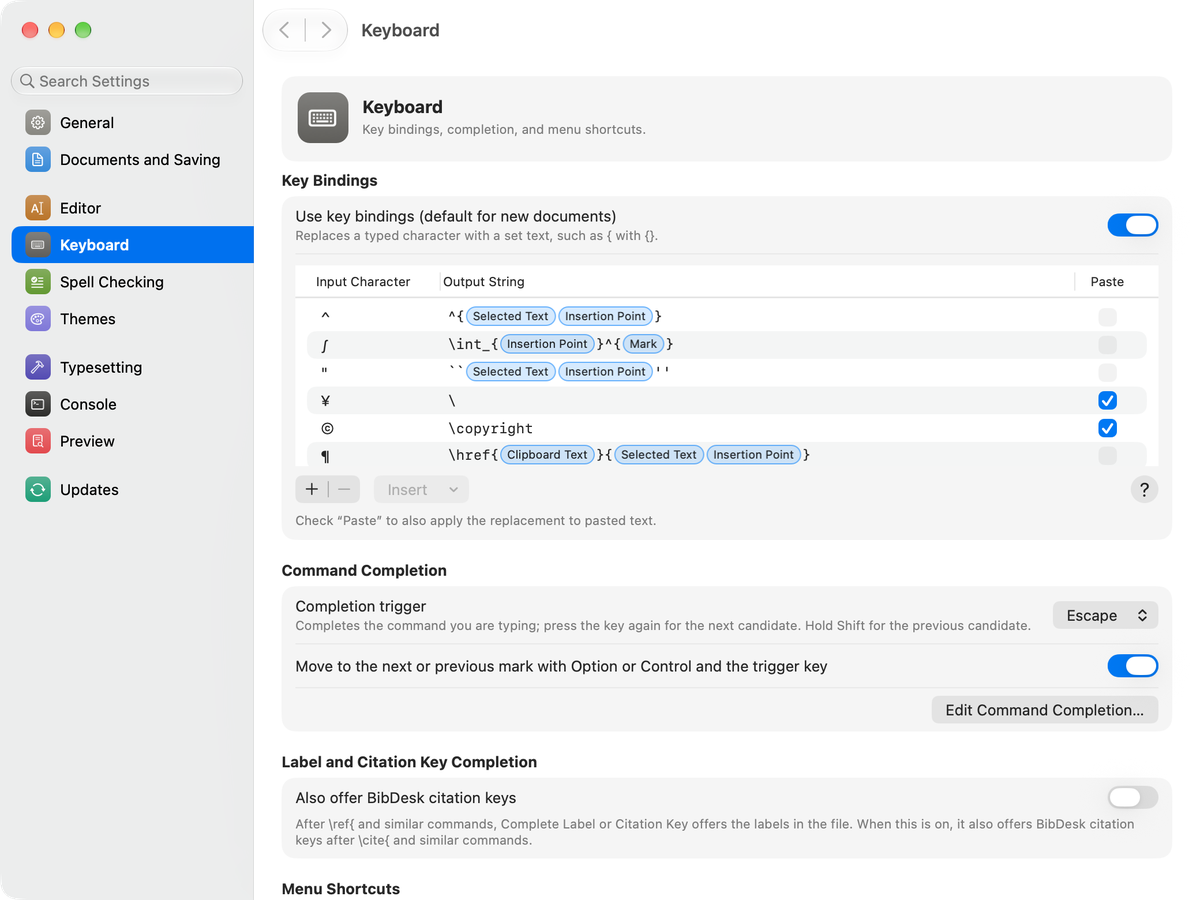
\includegraphics[width=4.5in]{Graphics/manual-key-bindings.png}
\caption{Key bindings and command completion in the Keyboard category of Settings}
\label{fig:KeyBindings}
\end{figure}

The \mnu{Key Bindings} group of the \mnu{Keyboard} category (\cref{fig:KeyBindings}) lists the key bindings, each \mnu{Input Character} with its \mnu{Output String}. Double-click a cell to edit it in place; click + below the list to add a key binding and $-$ to delete the selected ones, and drag rows to change their order. An input character is a single character. Changes are saved at once, and \mnu{Edit}\To\mnu{Undo} takes them back.

An output string can contain these symbols:
\begin{description}
\item[\texttt{\#SEL\#}] the text that was selected when the key was typed;
\item[\texttt{\#INS\#}] the place of the insertion point after the key binding;
\item[\texttt{\#PASTE\#}] the text on the clipboard;
\item[\texttt{•}] a mark, which \mnu{Edit}\To\mnu{Marks} can move to (\cref{MarksSection}).
\end{description}
In the list, these symbols, and line breaks and tabs, are shown as small labels such as \mnu{Selected Text}. Add them with the \mnu{Insert} menu below the list, or type them: the symbols as written above, a line break with Option-Return and a tab with Option-Tab. The \mnu{?} button beside the list shows all of them.

A check in the \mnu{Paste} column applies a key binding to pasted text as well: wherever its input character occurs in text pasted into the source, or dropped on it, the output string takes its place. As with typing, this happens only while key bindings are on for the document. A key binding whose output string contains \texttt{\#SEL\#}, \texttt{\#INS\#}, \texttt{\#PASTE\#} or a mark cannot be checked.

On a Japanese keyboard, the key for the backslash may type a yen sign (\textyen). In the list that comes with TeXShop, \textyen\ gives a single backslash and its \mnu{Paste} box is checked. So when the encoding for new documents is not a Japanese one, turning on key bindings is enough to have \textyen\ typed or pasted into the source become \verb|\|.

The list is kept in the folder \path{~/Library/TeXShop/Keyboard}, in \texttt{autocompletion.plist}, with the order of the rows and the checks of the \mnu{Paste} column in two more files beside it. To return to the list that comes with TeXShop, quit TeXShop, move the \texttt{Keyboard} folder to the desktop and start TeXShop again; it creates the folder with its default contents.

\section{Command Completion}\label{CommandCompletionSection}

Command completion enters commands and environments from their first letters or from a short abbreviation. It is always available, and is triggered by a key that is rarely typed otherwise: Escape, or Tab if you choose it under \mnu{Completion trigger} in the \mnu{Keyboard} category of TeXShop Settings. In this section the trigger key is written \esckey. The source panel of \mnu{Edit}\To\mnu{Experiment\ldots} uses the same key.

\subsection{Completing a Command}

Type the first letters of a command and press \esckey: TeXShop completes it from its completion list, \CCT. Press \esckey\ again to go through the other completions that begin with the same letters, from the bottom of the list toward the top; \shiftkey-\esckey\ goes the other way. One of the choices is the text you typed. For example, after
\begin{verbatim}
     \begin{th
\end{verbatim}
\esckey\ offers \verb|\begin{thebibliography}|, \verb|\begin{theindex}| and \verb|\begin{theorem}|. When the list has nothing for the text, the key does what it does elsewhere: Escape shows the word completions of macOS, and Tab types a tab.

A completion can do more than finish the word. The completion of \verb|\begin{theorem}| also writes the \verb|\end{theorem}| line, and puts marks (•) where you will type. The first mark is selected, shown here as \selmark, so what you type replaces it:
\begin{quote}\ttfamily
\textbackslash begin\{theorem\}\\
\selmark\\
\textbackslash end\{theorem\}•
\end{quote}
When the theorem is written, \mnu{Edit}\To\mnu{Marks}\To\mnu{Next Mark} (\ctlkey-\cmdkey-{]}), or \optkey-\esckey, selects the next mark, here the one after \verb|\end{theorem}|, so that you can go on typing; see \cref{MarksSection}.

Pressing \esckey\ several times often gives the same command with more arguments. Typing \verb|\newc| on a new line and pressing \esckey\ gives the first line below; further presses of \esckey\ give the others in turn, each with the first mark selected:
\begin{quote}\ttfamily
\textbackslash newcommand\{\selmark\}\{•\}\\
\textbackslash newcommand\{\selmark\}[•]\{•\}\\
\textbackslash newcommand\{\selmark\}[•][•]\{•\}
\end{quote}
Start typing the name of the new command to replace the selected mark, then move to the next mark and type the next argument. In the same way, \verb|\sec| gives in turn
\begin{quote}\ttfamily
\textbackslash section\{\selmark\}\\
\textbackslash section*\{\selmark\}\\
\textbackslash section[\selmark]\{•\}
\end{quote}
that is, the command, its starred form and the form with the optional argument.

It takes a little practice to learn which commands have completions. \verb|\begin{| alone has none; \verb|\begin{t| has many, and \verb|\begin{theo| only one. Learn the few that you need all the time and pick up others as you go.

\subsection{Abbreviations}

Besides the beginnings of commands, the list has many abbreviations: short names that stand for a longer command or a whole environment. The abbreviations of environments start with \texttt{b}. For example, \verb|benu| followed by \esckey\ at the start of a line gives a complete \texttt{enumerate} environment:
\begin{quote}\ttfamily
\textbackslash begin\{enumerate\}\\
\textbackslash item\\
\selmark\\
\textbackslash end\{enumerate\}•
\end{quote}
The final mark makes it easy to skip to the end of the environment with \mnu{Next Mark}. To add another item, type \verb|ite| and \esckey\ at the start of a new line, which gives \verb|\item| with a selected mark on the next line. Other abbreviations of environments are \verb|bite|, \verb|bali|, \verb|bfig|, \verb|btabl| and \verb|btab|, for the \texttt{itemize}, \texttt{align}, \texttt{figure}, \texttt{table} and \texttt{tabular} environments.

Sectioning commands have abbreviations too: \verb|sec|, \verb|ssec|, \verb|sssec|, \verb|par| and \verb|spar| give \verb|\section|, \verb|\subsection|, \verb|\subsubsection|, \verb|\paragraph| and \verb|\subparagraph|, with further variants on more presses of \esckey. The abbreviations of font commands are used inside a line, so they are typed with a backslash: \verb|\tt|, \verb|\sf|, \verb|\sc| and \verb|\bf| followed by \esckey\ give \verb|\texttt{|\selmark\verb|}|, \verb|\textsf{|\selmark\verb|}|, \verb|\textsc{|\selmark\verb|}| and \verb|\textbf{|\selmark\verb|}|, and \verb|\em| gives \verb|\emph{|\selmark\verb|}|.

The folder \path{~/Library/TeXShop/CommandCompletion} has the full documentation of the list, including a quick start guide.

\subsection{Marks with Notes}

Some completions say what belongs in an argument with a mark with a note, written •‹note›. This helps with commands whose arguments are easily forgotten. For example, \verb|\rul| and \esckey\ give the first line below, and a second \esckey\ the version with the optional argument:
\begin{quote}\ttfamily
\textbackslash rule\{\selcomrulewidth\}\{•‹height›\}\\
\textbackslash rule[\selcomrulelift]\{•‹width›\}\{•‹height›\}
\end{quote}
The selected mark and its note are replaced by what you type. The \texttt{wrapfigure} environment of the \texttt{wrapfig} package has several forms with different optional arguments; \verb|\bwr| and \esckey\ give the first,
\begin{quote}\ttfamily
\textbackslash begin\{wrapfigure\}\{\selcombwra\}\{•‹width›\}\\
•\\
\textbackslash end\{wrapfigure\}•
\end{quote}
and further presses of \esckey\ the others.

\subsection{Other Environments and Typing without a Backslash}

To close an environment that is not in the list, type \verb|\begin{|, the name of the environment and the closing brace, and press \esckey: the matching \verb|\end| line is added below, and the insertion point stays after \verb|\begin{name}|.

On some keyboards, typing \verb|\| takes several keystrokes. A completion need not start with a backslash: at the start of a line, after a space or a tab, or after punctuation such as \verb|(| or \verb|,|, \verb|sec| and \esckey\ give the same as \verb|\sec|, and \verb|tt| gives \verb|\texttt{|\selmark\verb|}|. After other characters, such as \verb|`| in \verb|`tt|, the backslash is needed. A macro that inserts only a backslash, with a simple keyboard shortcut, also helps (\cref{MacrosChapter}).

\subsection{Changing the Completion List}

To add text to the completion list, select it and choose \mnu{Source}\To\mnu{Add to Command Completion List} (\shiftkey-\cmdkey-W); it is added at the end of the list, and the previous list is kept as \texttt{CommandCompletion\textasciitilde.txt}. To edit the list, click \mnu{Edit Command Completion\ldots} in the \mnu{Keyboard} category of TeXShop Settings; the list opens in TeXShop as a text file.

Studying the completions that are there is the best way to learn how to write new ones. Each line is one completion. A line such as \verb|\emph{#INS#•#INS#}| completes the text it begins with; a line such as \verb|benu:=\begin{enumerate}...| completes the abbreviation before \verb|:=| with the text after it. In that text, \verb|#RET#| is a line break, a mark • is a mark, and the text between two \verb|#INS#| is selected after the completion; a single \verb|#INS#| places the insertion point. For files highlighted as XML, TeXShop uses the list \texttt{CommandCompletionXML.txt} in the same folder. The folder also holds other versions of the list, with their own systematic ways of naming abbreviations.

\section{Marks}\label{MarksSection}

A mark (•) is a place to come back to; a mark with a note (•‹note›) also says what belongs there. Command completions, macros and key bindings can contain marks, and you can insert them yourself. The commands are in \mnu{Edit}\To\mnu{Marks}:
\begin{description}
\item[Insert Mark] (\cmdkey-8) inserts a mark.
\item[Insert Mark with Note] (\ctlkey-\cmdkey-8) inserts •‹› with the insertion point between the brackets, or turns the selected text into the note.
\item[Next Mark] (\ctlkey-\cmdkey-{]}) and \textbf{Previous Mark} (\ctlkey-\cmdkey-{[}) select the next or the previous mark together with its note, so that typing replaces it.
\item[Next Mark (Del)] and \textbf{Previous Mark (Del)}, shown while the Option key is held down (\ctlkey-\optkey-\cmdkey-{]} and \ctlkey-\optkey-\cmdkey-{[}), delete the • and select the note instead.
\item[How to Use Marks\ldots] opens the help page about marks.
\end{description}

The trigger key of command completion moves between marks too: with Escape as the trigger, \optkey-\esckey\ goes to the next mark and \ctlkey-\esckey\ to the previous one; with Tab, \optkey-\tabkey\ and \ctlkey-\tabkey. If another application needs these keys, turn off \mnu{Move to the next or previous mark with Option or Control and the trigger key} in the \mnu{Keyboard} category of TeXShop Settings.

\section{Label and Citation Key Completion}\label{LabelCompletionSection}

\mnu{Edit}\To\mnu{Complete Label or Citation Key} (F5) completes a label or a citation key from a list. Choose it right after \texttt{\textbackslash ref\{}, \texttt{\textbackslash pageref\{}, \texttt{\textbackslash eqref\{} or \texttt{\textbackslash autoref\{}, or after the first letters of a label typed there, and a list of the labels defined with \verb|\label| in the file appears. Select a label with the arrow keys and press Return to enter it.

After \texttt{\textbackslash cite\{} and similar commands, the list shows citation keys from BibDesk. This happens only when \mnu{Also offer BibDesk citation keys}, in the group \mnu{Label and Citation Key Completion} of the \mnu{Keyboard} category of TeXShop Settings, is on, and BibDesk must be installed. Elsewhere, the list shows the word completions of macOS.

On many keyboards the top row of keys controls the brightness, the sound and other features of the Mac; then hold down the fn key (the Globe key) while pressing F5, or give the command another shortcut (\cref{KeyboardChapter}).

\section{Tags and Labels}\label{TagsSection}

The \mnu{Tags} item of the source window's toolbar is a menu of the chapters, sections and other divisions of the document; choose one to go to that place in the source. It lists the commands \verb|\part|, \verb|\chapter|, \verb|\section|, \verb|\subsection|, \verb|\subsubsection|, \verb|\paragraph|, \verb|\subparagraph| and \verb|\frametitle|, the environments \texttt{frame}, \texttt{slide}, \texttt{wideslide} and \texttt{notes}, and, for documented \texttt{.dtx} sources, these commands and the \texttt{macro} and \texttt{environment} environments in lines beginning with \verb|% |. A command is listed only when it starts its line. In XML files the menu lists the tags checked in the group \mnu{XML Tags in the Tag List} of the \mnu{Editor} category of TeXShop Settings.

To add a tag of your own, start a line with \verb|%:| followed by its name, for example \verb|%: Proof of the main theorem|. \mnu{Source}\To\mnu{User Location Mark} (\cmdkey-2) inserts a new line with \verb|%:| above the current line and leaves the insertion point after it, so that you can type the name of the tag.

The \mnu{Labels} item of the toolbar works in the same way and lists the \verb|\label|s of the source. \mnu{Tags Menu in Menubar}, in the \mnu{Display} group of the \mnu{Editor} category of TeXShop Settings, adds the Tags menu to the menu bar as well.

\section{Showing Invisible Characters}\label{ShowInvisibleSection}

\mnu{Source}\To\mnu{Show Invisible Characters} (\ctlkey-\cmdkey-I) shows spaces, Japanese (fullwidth) spaces, line ends and tabs as visible symbols, in the \mnu{Invisible} color of the theme. Which of these characters are shown, and with which symbol, is set in the \mnu{Invisible} group of the \mnu{Editor} category of TeXShop Settings; \mnu{Show Invisible Characters} in the group \mnu{When a Document Opens} of the same category sets whether a document starts with them shown.

Control characters other than tab, line feed and carriage return are always shown, as the replacement character U+FFFD in the \mnu{Invisible} color, whether or not invisible characters are shown. They are usually left over from text copied out of other programs, and \TeX\ reports them as errors.

\section{Highlighting Fullwidth Characters}\label{FullwidthHighlightSection}

Fullwidth letters, digits and symbols, which a Japanese input method easily produces, and the minus sign U+2212 look much like their ASCII counterparts, but \TeX\ treats them as different characters: a fullwidth brace, for example, does not end an argument. The source shows these characters in the \mnu{Fullwidth} and \mnu{Fullwidth (Background)} colors of the theme, so that they stand out. To show them like other text, turn off \mnu{Highlight Fullwidth Letters and Symbols} in the \mnu{Syntax Highlighting} group of the \mnu{Editor} category of TeXShop Settings; the colors themselves are set in the \mnu{Themes} category (\cref{ThemeColorsSection}). To replace such characters by ordinary ones, use \mnu{Edit}\To\mnu{Character Type Conversion} (\cref{CharacterConversionSection}).

\section{Highlighting the Current Line and the Block Cursor}\label{BlockCursorSection}

Two features make the insertion point easier to find. \mnu{Source}\To\mnu{Highlight Current Line} gives the line that holds the insertion point a background of its own, the \mnu{Current Line} color in the \mnu{Source} group of the \mnu{Themes} category of TeXShop Settings. If you start a new line only at the end of a paragraph, the highlighted ``line'' is the whole paragraph.

\mnu{Source}\To\mnu{Use Block Insertion Cursor} gives the characters next to the insertion point a colored background, so that the insertion point stands out like the block cursor of Terminal. Only one of the two is shown at a time: the block cursor replaces the highlight of the current line.

Both menu items act on the document in front. In the \mnu{Editor} category of Settings, \mnu{Highlight Current Line} and \mnu{Use Block Cursor} in the group \mnu{When a Document Opens} set how documents start. The \mnu{Insertion} group of the same category sets the \mnu{Cursor Color}, and with \mnu{Side of Insertion Line} whether the character on the \mnu{Left}, on the \mnu{Right} or on \mnu{Both Sides} of the insertion point is colored; \mnu{Width for Left or Right} colors one or two characters when a single side is chosen.

\section{The Clipboard}\label{ClipboardSection}

\subsection{Swap with Clipboard}

\mnu{Edit}\To\mnu{Swap with Clipboard} replaces the selected text with the text on the clipboard, and puts the text it replaced on the clipboard. To exchange two pieces of text, copy the first piece, select the second and choose \mnu{Swap with Clipboard}, then select the place of the first piece and paste. When nothing is selected, the command is an ordinary paste. It has no keyboard shortcut at first; give it one in the \mnu{Keyboard} category of TeXShop Settings (\cref{KeyboardChapter}) if you use it often.

\subsection{Copy with Style}\label{CopyWithStyleSection}

The submenu \mnu{Edit}\To\mnu{Copy with Style} copies the selected text in the font of the source and with the colors of a theme, to paste it into a word processor, a presentation or an email. Its four items, \mnu{Light Mode Theme}, \mnu{Light Mode Theme with Background}, \mnu{Dark Mode Theme} and \mnu{Dark Mode Theme with Background}, choose the theme set for Light Mode or for Dark Mode in the \mnu{Themes} category of TeXShop Settings, and whether the background color of the source is copied too, whatever the appearance TeXShop is shown in. The Light Mode theme without background suits a white page; the Dark Mode theme with background shows the source as a dark block.

The text keeps the colors of syntax highlighting and of fullwidth letters and symbols; the highlights of the current line, of braces and of found text are not copied. The text goes to the clipboard as rich text (RTF and HTML) and as plain text, so applications that take only plain text paste it without colors. \mnu{Edit}\To\mnu{Copy} still copies plain text only. The items have no keyboard shortcuts; each can be given one in the \mnu{Keyboard} category of TeXShop Settings.

\section{Character Type Conversion and Unicode Normalization}\label{CharacterConversionSection}

Two submenus of the \mnu{Edit} menu, \mnu{Character Type Conversion} and \mnu{Unicode Normalization}, rewrite the selected text; they are also in the contextual menu of the source. If nothing is selected, TeXShop asks whether to apply the command to the whole document. Each command can be undone.

\mnu{Character Type Conversion} is mainly useful for Japanese documents. Its items convert
\begin{itemize}
\item between hiragana and katakana (\mnu{Hiragana \(\to\) Katakana}, \mnu{Katakana \(\to\) Hiragana}),
\item between fullwidth and halfwidth digits (\mnu{Fullwidth Digits \(\to\) Halfwidth Digits} and back), and between fullwidth and halfwidth Latin letters (\mnu{Fullwidth Letters \(\to\) Halfwidth Letters} and back),
\item between circled and parenthesized numbers and letters, Roman numerals and similar characters, and the commands of the \texttt{ajmacros} package that print them, for example \verb|\ajMaru{1}| for a circled~1 (\mnu{Unicode Characters \(\to\) ajmacros} and \mnu{ajmacros \(\to\) Unicode Characters}),
\item between characters outside the JIS~X~0208 character set and the \verb|\UTF{...}| and \verb|\CID{...}| commands of the \texttt{otf} package for pLaTeX and upLaTeX (\mnu{Unicode Characters \(\to\) \textbackslash UTF / \textbackslash CID} and \mnu{\textbackslash UTF / \textbackslash CID \(\to\) Unicode Characters}),
\item from curly quotation marks to the \TeX\ forms \verb|`|, \verb|'|, \verb|``| and \verb|''| (\mnu{Curly Quotes \(\to\) TeX Quotes}).
\end{itemize}
The same conversions between Unicode characters and \texttt{ajmacros} are available as sample sets of Multiple Replace (\cref{MultipleReplaceSection}).

\mnu{Unicode Normalization} converts the selection to one of the Unicode normalization forms \mnu{NFC}, \mnu{NFD}, \mnu{NFKC} and \mnu{NFKD}. In NFC a letter followed by a combining accent becomes a single precomposed character; NFD decomposes such characters. NFKC and NFKD also replace compatibility characters, such as ligatures and fullwidth letters, by their ordinary equivalents. \mnu{Modified NFC} and \mnu{Modified NFD} work like NFC and NFD, but leave CJK compatibility ideographs and a few other characters unchanged, because NFC and NFD would replace them by different ideographs. Modified NFD is the decomposition used for file names on HFS+ disks, and Modified NFC is the form TeXShop writes when \mnu{Automatically convert UTF-8-MAC to UTF-8} is on in the \mnu{Documents and Saving} category of TeXShop Settings. Since normalized text usually looks the same as before, TeXShop shows the Character Info panel (\cref{CharacterInfoSection}) for the selection afterward, with the code points of the result. (See also \cref{JapanChapter}.)

\section{The Status Bar and Text Statistics}\label{CountingWordsSection}

The status bar under the source (\cref{fig:StatusBar}) shows, from the left, the number of \mnu{Lines}, \mnu{Characters} and \mnu{Words} in the document, each followed in parentheses by the number in the selection when text is selected; then the \mnu{Location}, \mnu{Line} and \mnu{Column} of the insertion point; and at the right the size of the saved file. The numbers follow the text as you type. Characters are counted as they are seen, so an accented letter or an emoji counts as one, and \LaTeX\ commands are counted as they are written. Words are found as in other Mac applications. \mnu{Source}\To\mnu{Show Status Bar} shows or hides the status bar in all source windows at once.

\begin{figure}[htbp]
\centering
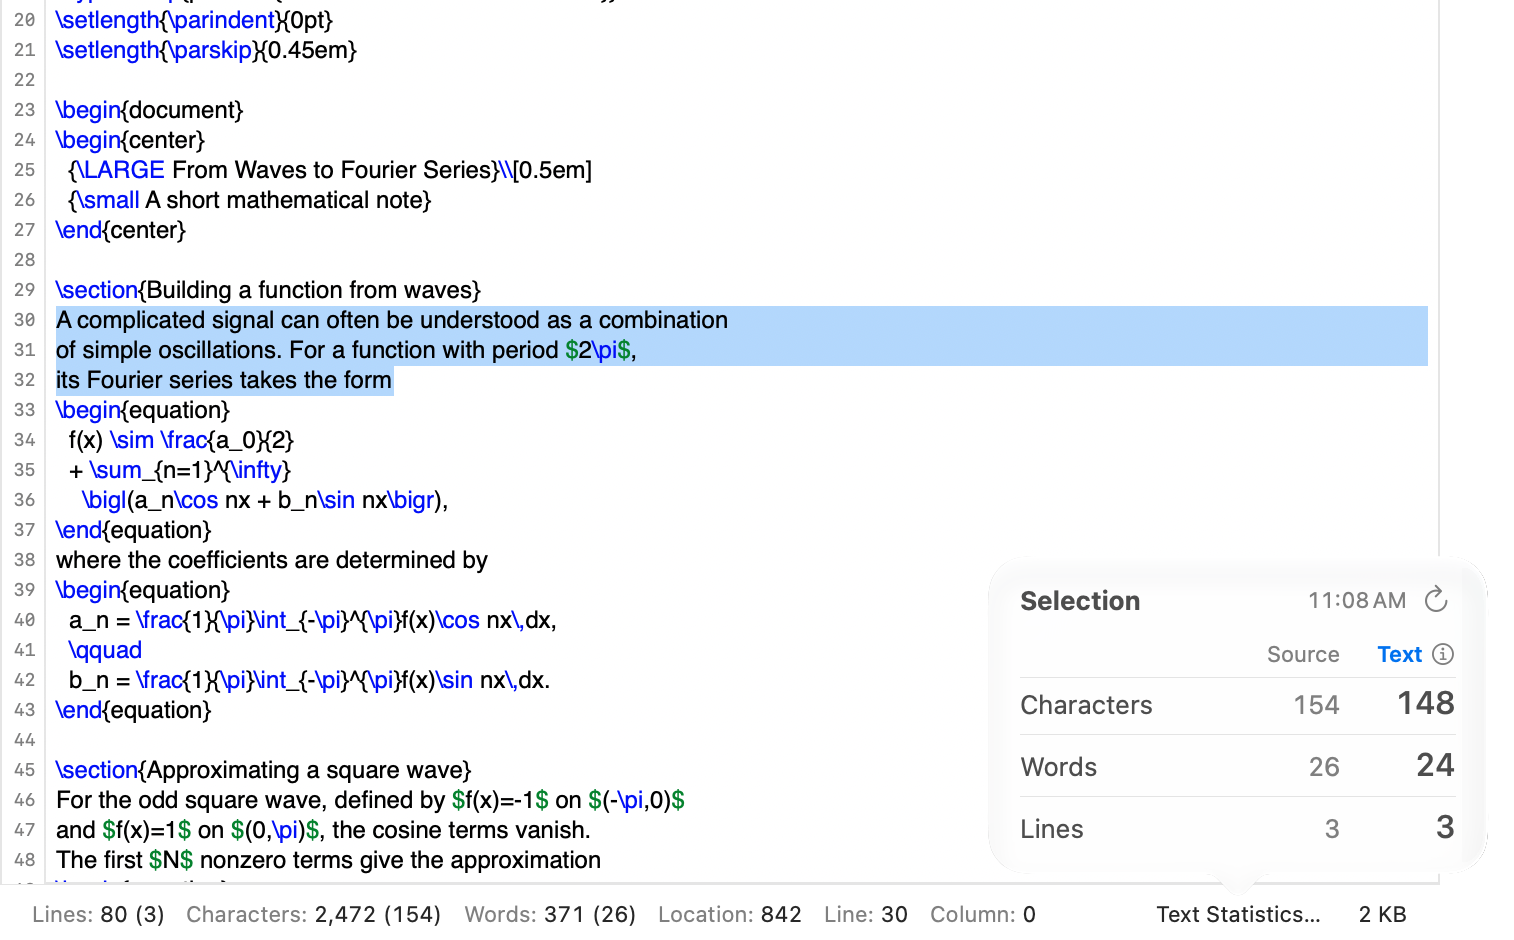
\includegraphics[width=4.5in]{Graphics/manual-status-bar.png}
\caption{The status bar under the source, and Text Statistics opened from it}
\label{fig:StatusBar}
\end{figure}

To count the text without the \LaTeX\ commands, click \mnu{Text Statistics\ldots} in the status bar, or choose \mnu{Edit}\To\mnu{Statistics\ldots}. A popover shows the numbers of \mnu{Characters}, \mnu{Words} and \mnu{Lines} of the \mnu{Whole Document}, or of the \mnu{Selection} when text is selected, in two columns. \mnu{Source} is the source as it is written. \mnu{Text} is what remains after \cmd{detex}, a program in \TeX\ Live, removes the commands; the files read with \verb|\input| and \verb|\include| are counted too. The document need not be saved. The time at the top of the popover tells when the numbers were counted; click the refresh button beside it to count again after editing.

\subsection{Character Count Options}\label{CharacterCountOptionsSection}

The options button beside the refresh button shows how the characters are counted, under the numbers (\cref{fig:TextStatisticsOptions}); click it again to hide them. When an option changes, the numbers of the \mnu{Characters} row change at once.

\begin{figure}[htbp]
\centering
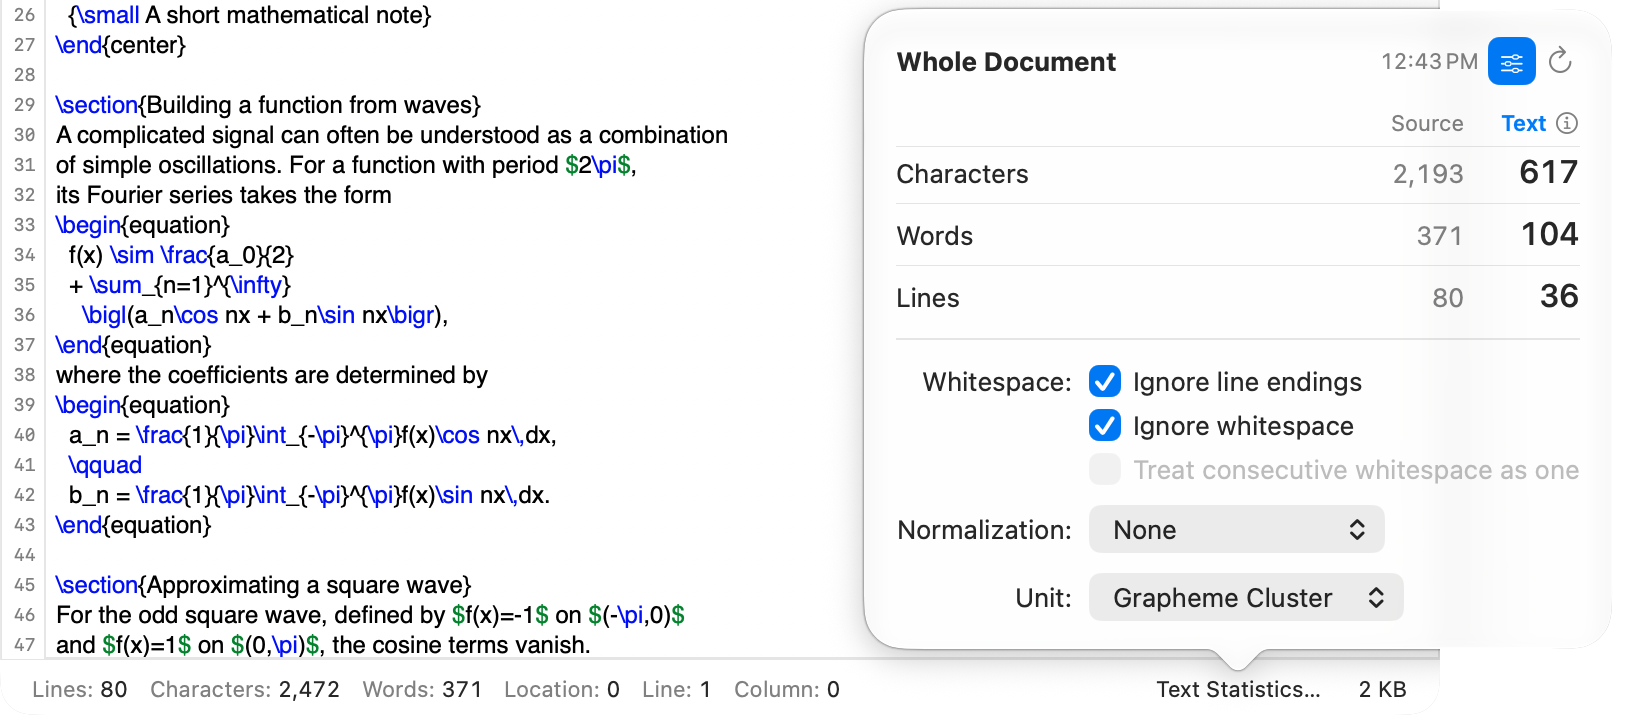
\includegraphics[width=4.5in]{Graphics/manual-text-statistics.png}
\caption{Text Statistics with its options shown: line endings and whitespace are not counted}
\label{fig:TextStatisticsOptions}
\end{figure}

\begin{itemize}
\item \mnu{Ignore line endings} leaves the line endings out of the count, and \mnu{Ignore whitespace} the spaces and tabs, the ideographic space among them. \mnu{Treat consecutive whitespace as one} counts a run of two or more spaces and line endings as one space.
\item \mnu{Normalization} converts the text to \mnu{NFC}, \mnu{NFD}, \mnu{NFKC}, \mnu{NFKD}, \mnu{NFKC Case-Fold}, \mnu{Modified NFC} or \mnu{Modified NFD} before counting (\cref{CharacterConversionSection}); NFKC Case-Fold also folds upper case to lower case and drops invisible characters such as soft hyphens. The source itself is not changed.
\item \mnu{Unit} chooses what is counted: \mnu{Grapheme Cluster}, characters as they are seen; \mnu{Unicode Scalar}, the Unicode code points; \mnu{UTF-16}, the UTF-16 code units; or \mnu{Byte}, the bytes of the text in the encoding chosen in \mnu{Encoding}. The first row is then named after the unit. A dash shows that some characters cannot be written in the encoding.
\end{itemize}

The options are the same for all documents and are kept when TeXShop quits; the encoding is the document's each time the popover opens. While the options are hidden, the options button is shown in color when the characters are not counted as the status bar counts them.

% ===== 13-find.tex
\chapter{Find and Replace}\label{FindChapter}

TeXShop finds and replaces text in the source with the Advanced Find Panel. The panel finds plain text or regular expressions, lists all matches, highlights them in the text, and replaces them one by one or all at once. Two more tools are built on it: Multiple Replace applies a saved list of replacements in one step (\cref{MultipleReplaceSection}), and Find in TeX Sources finds and replaces in all the files of a document split into chapter files (\cref{TeXRootSearchSection}).

The commands for finding are in the submenu \mnu{Edit}\To\mnu{Find}. This chapter is about finding text in the source. Finding text in the typeset document is described with the Preview window (\cref{PreviewChapter}). TeXShop can also use other find interfaces instead of the Advanced Find Panel (\cref{FindInterfaceSection}).

\section{The Advanced Find Panel}\label{AdvancedFind}

\begin{figure}[htbp]
\centering
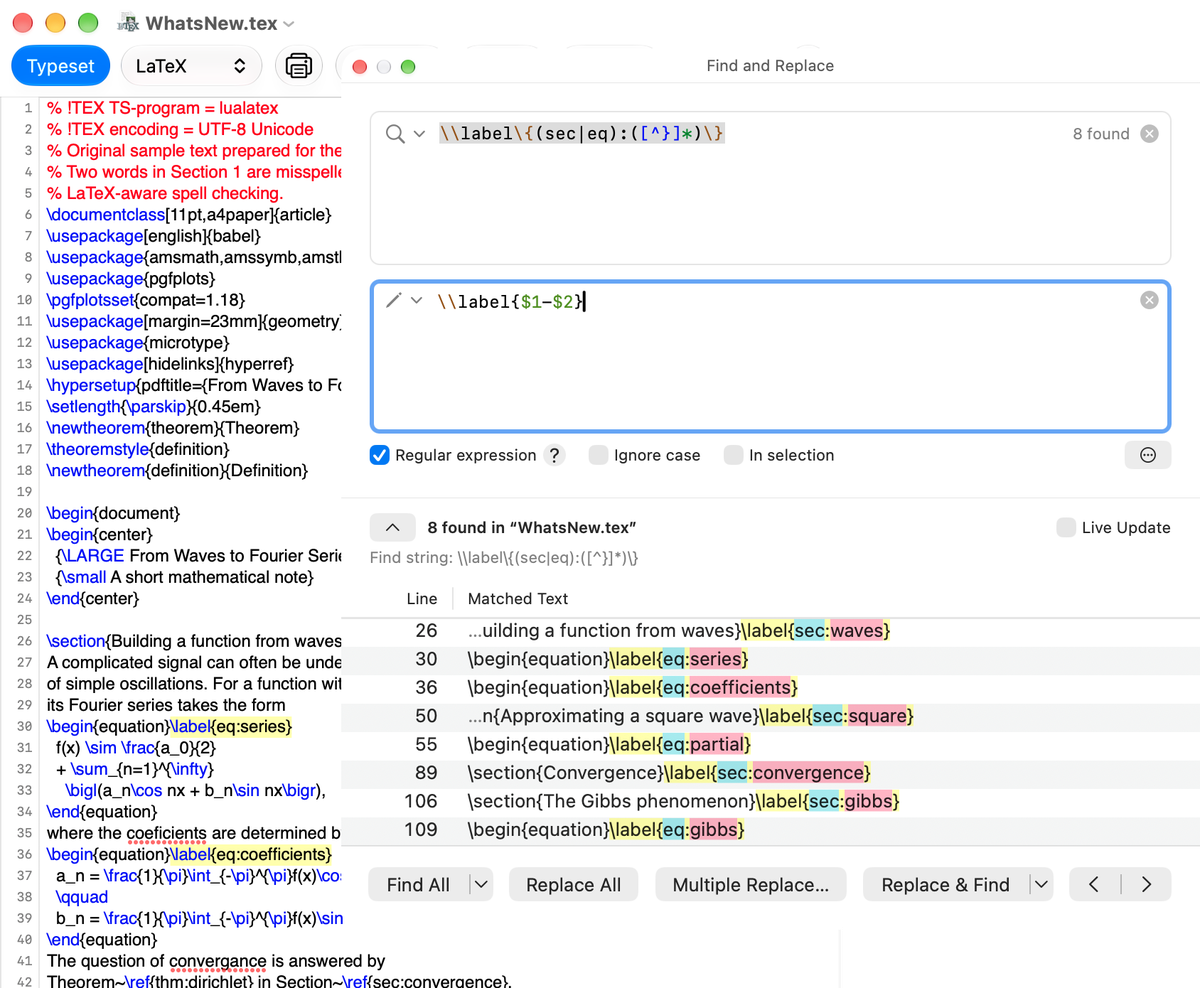
\includegraphics[width=4.7in]{Graphics/manual-advanced-find.png}
\caption{The Advanced Find Panel with the list of Find All}
\label{fig:AdvancedFind}
\end{figure}

The panel (\cref{fig:AdvancedFind}) has, from the top, the find field, the replacement field, a row of options, the list of matches made by \mnu{Find All}, and a row of buttons. It acts on the source window in front.

\subsection{Opening the Panel and the Find Menu}\label{sec:FindMenu}

\begin{figure}[htbp]
\centering
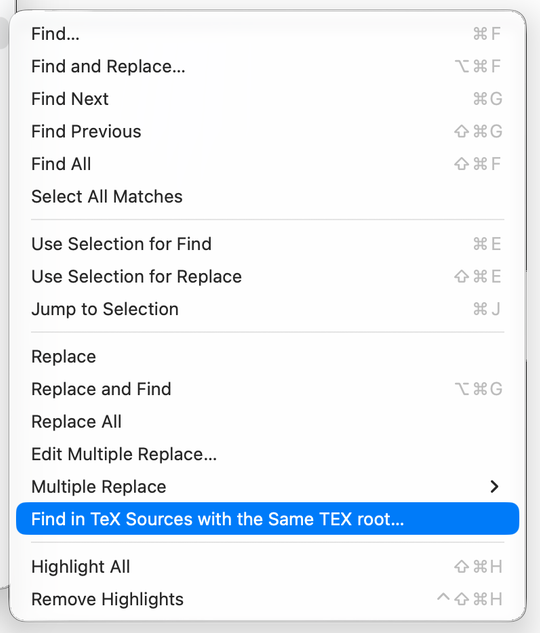
\includegraphics[width=3.2in]{Graphics/manual-find-menu.png}
\caption{The Find submenu of the Edit menu}
\label{fig:FindMenu}
\end{figure}

The \mnu{Find} submenu of the \mnu{Edit} menu (\cref{fig:FindMenu}) has these commands. All except the first two also work while the panel is closed.
\begin{description}
\item[\mnu{Find\ldots} (\cmdkey-F)] opens the panel with the find field selected.
\item[\mnu{Find and Replace\ldots} (\optkey-\cmdkey-F)] opens the panel with the replacement field selected.
\item[\mnu{Find Next} (\cmdkey-G) and \mnu{Find Previous} (\shiftkey-\cmdkey-G)] select the next or the previous match in the source.
\item[\mnu{Find All} (\shiftkey-\cmdkey-F)] lists all matches in the panel (\cref{sec:FindAllList}).
\item[\mnu{Select All Matches}] selects all matches in the source at once, so that they can be typed over together.
\item[\mnu{Use Selection for Find} (\cmdkey-E) and \mnu{Use Selection for Replace} (\shiftkey-\cmdkey-E)] put the text selected in the source into the find field or the replacement field.
\item[\mnu{Jump to Selection} (\cmdkey-J)] scrolls the source so that the selection is visible.
\item[\mnu{Replace}, \mnu{Replace and Find} (\optkey-\cmdkey-G) and \mnu{Replace All}] replace the selected match, replace it and select the next one, or replace all matches.
\item[\mnu{Edit Multiple Replace\ldots} and \mnu{Multiple Replace}] open the Multiple Replace window and apply one of its sets (\cref{MultipleReplaceSection}).
\item[\mnu{Find in TeX Sources with the Same TEX root\ldots}] finds and replaces in all the files of a document (\cref{TeXRootSearchSection}).
\item[\mnu{Highlight All} (\shiftkey-\cmdkey-H) and \mnu{Remove Highlights} (\ctlkey-\shiftkey-\cmdkey-H)] mark all matches in the text and remove the marks (\cref{sec:FindHighlights}).
\end{description}
Commands that cannot act, for example \mnu{Replace} when nothing is selected, are dimmed. Every shortcut can be changed in the \mnu{Keyboard} category of TeXShop Settings (\cref{KeyboardChapter}).

\subsection{The Find and Replacement Fields}

Type the text to find in the upper field and the replacement in the lower one. Both fields can hold several lines, and they grow when the panel is made larger. In a field, Return finds the next match and Tab moves to the other field; \optkey-Return and \optkey-Tab insert a line break and a tab.

While you type in the find field, the panel already selects the next match in the source. (The hidden setting \texttt{IncrementalSearch} turns this off; see \cref{chap:hidden-settings}.) The right end of the find field shows the result, for example ``3 of 12'' for the position of the current match, or ``Not found''. The button with a cross at the right end empties the field.

The icon with a small arrow at the left of each field opens the list of recent strings of that field; choose one to use it again. \mnu{Clear Recent Searches} or \mnu{Clear Recent Replacements} at the end of the list removes them.

The fields use a monospaced font at about the size of the source font, so that \verb+|+ and \verb+l+ or \verb+0+ and \verb+O+ are not confused, and the colors of the current theme (\cref{ThemesChapter}). With \mnu{Regular expression} off, the text in them is colored as \TeX\ is in the source. With \mnu{Regular expression} on, they show the parts of a pattern in colors of their own: character classes, repetitions, groups, escapes, anchors and references. A mistake, such as a group that is not closed or a reference in the replacement to a group the pattern does not have, is red and underlined; what the OgreKit Find Panel would read differently is orange with a dotted underline. The line below the options explains the first mark and says how many more there are. In the find field, when the insertion point is right after a parenthesis or a square bracket of the pattern, its partner is shown briefly, and a double-click on one selects the pair with what is between.

\subsection{Options}\label{sec:FindOptions}

Below the fields are three check boxes:
\begin{description}
\item[\mnu{Regular expression}] reads the find string as a pattern (\cref{RegularExpressionsSection}). The small \mnu{?} button next to it opens the Regular Expression Reference.
\item[\mnu{Ignore case}] treats capital and small letters as the same.
\item[\mnu{In selection}] finds and replaces only in the text selected in the source.
\end{description}

\begin{figure}[htbp]
\centering
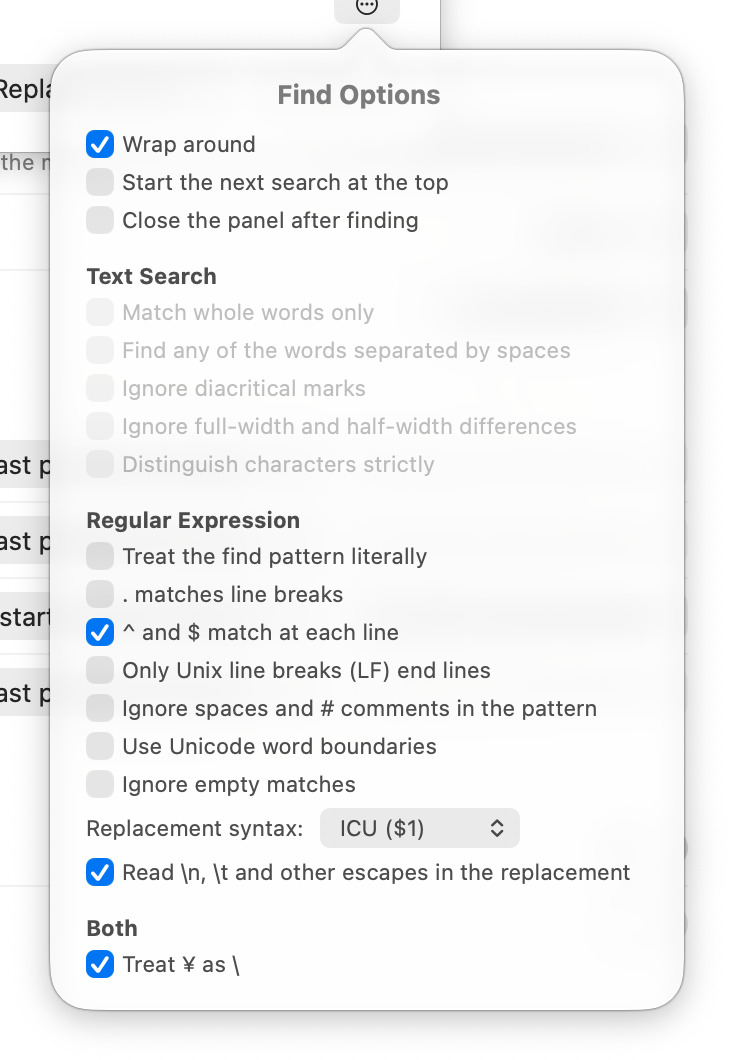
\includegraphics[width=2.8in]{Graphics/manual-find-options.png}
\caption{More Options of the Advanced Find Panel}
\label{fig:FindOptions}
\end{figure}

The button with three dots at the right of the row (\mnu{More Options}) shows the other options (\cref{fig:FindOptions}). At the top:
\begin{itemize}
\item \mnu{Wrap around}: after the last match, \mnu{Find Next} goes on from the start of the text, and \mnu{Find Previous} likewise from the end.
\item \mnu{Start the next search at the top}: the next search starts at the beginning of the text rather than at the selection.
\item \mnu{Close the panel after finding}: the panel closes after it has found a match, so that you can go on typing in the source.
\end{itemize}
Under \mnu{Text Search}, the options used when \mnu{Regular expression} is off:
\begin{itemize}
\item \mnu{Match whole words only}: \verb|sec| does not find the start of \verb|section|.
\item \mnu{Find any of the words separated by spaces}: \verb|theorem lemma| finds both words.
\item \mnu{Ignore diacritical marks}: \verb|e| also finds \verb|é| and \verb|è|.
\item \mnu{Ignore full-width and half-width differences}: a letter or a digit also finds its full-width form, as used in Japanese text.
\item \mnu{Distinguish characters strictly}: characters are compared code point by code point, so that for example an accented letter written as one character and the same letter written as a letter and a combining accent are different.
\end{itemize}
Under \mnu{Regular Expression}, the options used when \mnu{Regular expression} is on:
\begin{itemize}
\item \mnu{Treat the find pattern literally}: the characters of the pattern have no special meaning.
\item \mnu{. matches line breaks}.
\item \mnu{\textasciicircum{} and \$ match at each line}: on by default; when it is off, they match only at the start and the end of the whole text.
\item \mnu{Only Unix line breaks (LF) end lines}.
\item \mnu{Ignore spaces and \# comments in the pattern}, for long patterns written over several lines.
\item \mnu{Use Unicode word boundaries} for \verb|\b|.
\item \mnu{Ignore empty matches}, such as those of \verb|x*| between two characters.
\item \mnu{Replacement syntax}: \mnu{ICU (\$1)} or \mnu{OgreKit (\textbackslash 1)} (\cref{RegularExpressionsSection}).
\item \mnu{Read \textbackslash n, \textbackslash t and other escapes in the replacement}.
\end{itemize}
Under \mnu{Both}, \mnu{Treat \textyen\ as \textbackslash}, on by default, lets a \textyen\ typed on a Japanese keyboard stand for a backslash.

The options are kept from one session to the next.

\subsection{The Buttons}

The buttons at the bottom of the panel are:
\begin{description}
\item[\mnu{Find All}] lists every match in the panel (\cref{sec:FindAllList}). The arrow at its right opens a menu with \mnu{Highlight All}, \mnu{Select All}, \mnu{Remove Highlights}, and \mnu{Find in TeX Sources with the Same TEX root\ldots} (\cref{TeXRootSearchSection}).
\item[\mnu{Replace All}] replaces every match, or every match in the selection when \mnu{In selection} is on. A single Undo takes back the whole replacement.
\item[\mnu{Multiple Replace\ldots}] opens the Multiple Replace window (\cref{MultipleReplaceSection}).
\item[\mnu{Replace \& Find}] replaces the selected match and selects the next one. The arrow at its right opens a menu with \mnu{Replace}, which replaces without going on.
\item[The two arrows] select the previous and the next match.
\end{description}

\subsection{The List of Matches}\label{sec:FindAllList}

\mnu{Find All} opens a list under the options (\cref{fig:AdvancedFind}). Its heading says how many matches were found in which document, and the line below repeats the find string. The list has a row for each match, with the line number and the text of the line; the match is marked, and with a regular expression each group of the pattern has a color of its own.

Click a row to select its match in the source; double-click it to bring the source window to the front as well. The arrow keys move through the list from match to match.

When you edit the text, the rows whose match was changed turn gray, and the heading says how many changed. With \mnu{Live Update} on, the list is made again shortly after each edit. The arrow button at the left of the heading closes the list.

\subsection{Highlighting Matches}\label{sec:FindHighlights}

\mnu{Highlight All}, in the menu of \mnu{Find All} or in the \mnu{Find} submenu, marks every match in the text with a colored background, so that you see at a glance where a command or a word is used. With \mnu{Regular expression} on, the groups of the pattern are shown in their own colors, as in the Find All list. The marks are drawn over the colors the source already has, follow your edits, and appear in both parts of a split window. \mnu{Remove Highlights} removes them.

\subsection{Long Operations}

\mnu{Find All}, \mnu{Replace All} and Multiple Replace work in the background. Until they end, the document cannot be edited. When one takes long, a sheet on the document window shows its name, a progress bar and the number of matches found so far. The button with a cross in the sheet, or the Escape key, cancels it and leaves the text as it was.

\subsection{Finding in the Console, the Log and Experiments}

The panel also finds text in the console, the log, and the source panel and the console of \mnu{Experiment} (\cref{ConsoleSection,ExperimentsSection}). Click in one of them and use the panel or the \mnu{Find} submenu as in a source window; \mnu{Find All} and \mnu{Highlight All} work there too. The console, the log and the Experiment console show the output of \TeX, so the commands and buttons that replace are dimmed there.

\subsection{Keeping the Panel in Front}

The panel is one of the document windows: a click in the source window puts it behind that window, and \mnu{Find} brings it back. To keep it in front of the document windows, turn on \mnu{Keep the Advanced Find panel on top} in the \mnu{Find} group of the \mnu{Editor} category of TeXShop Settings.

\section{Regular Expressions}\label{RegularExpressionsSection}

With \mnu{Regular expression} on, the find string is a pattern in the syntax of ICU, the regular expressions of macOS. Most patterns are written as in other applications. The differences from the OgreKit Find Panel that matter most:
\begin{itemize}
\item A brace that does not belong to a repetition must be written \verb|\{| or \verb|\}|. For example, search for \verb|\\section\{| rather than \verb|\\section{|.
\item \verb|\d|, \verb|\w|, \verb|\s| and \verb|\b| also match full-width digits, kanji, kana and full-width spaces.
\item \verb|\h|, \verb|\K|, \verb|\g<name>| and \verb|(?m)| do not mean what they mean in OgreKit.
\end{itemize}

In the replacement, with the ICU syntax, \verb|$0| is the whole match and \verb|$1|, \verb|$2|, \ldots\ are the groups, and \verb|\$| is a dollar sign, so a formula \verb|$x$| is written \verb|\$x\$|. With the OgreKit syntax, \verb|\0| or \verb|\&| is the whole match, \verb|\1|, \verb|\2|, \ldots\ are the groups, \verb|\g<name>| is a named group, and \verb|$| is an ordinary character. In both, a backslash is written twice: \verb|\\section| gives \verb|\section|. The syntax is chosen with \mnu{Replacement syntax} among the options (\cref{sec:FindOptions}). The ICU syntax is the default; users who came from the OgreKit Find Panel start with the OgreKit syntax.

\begin{figure}[htbp]
\centering
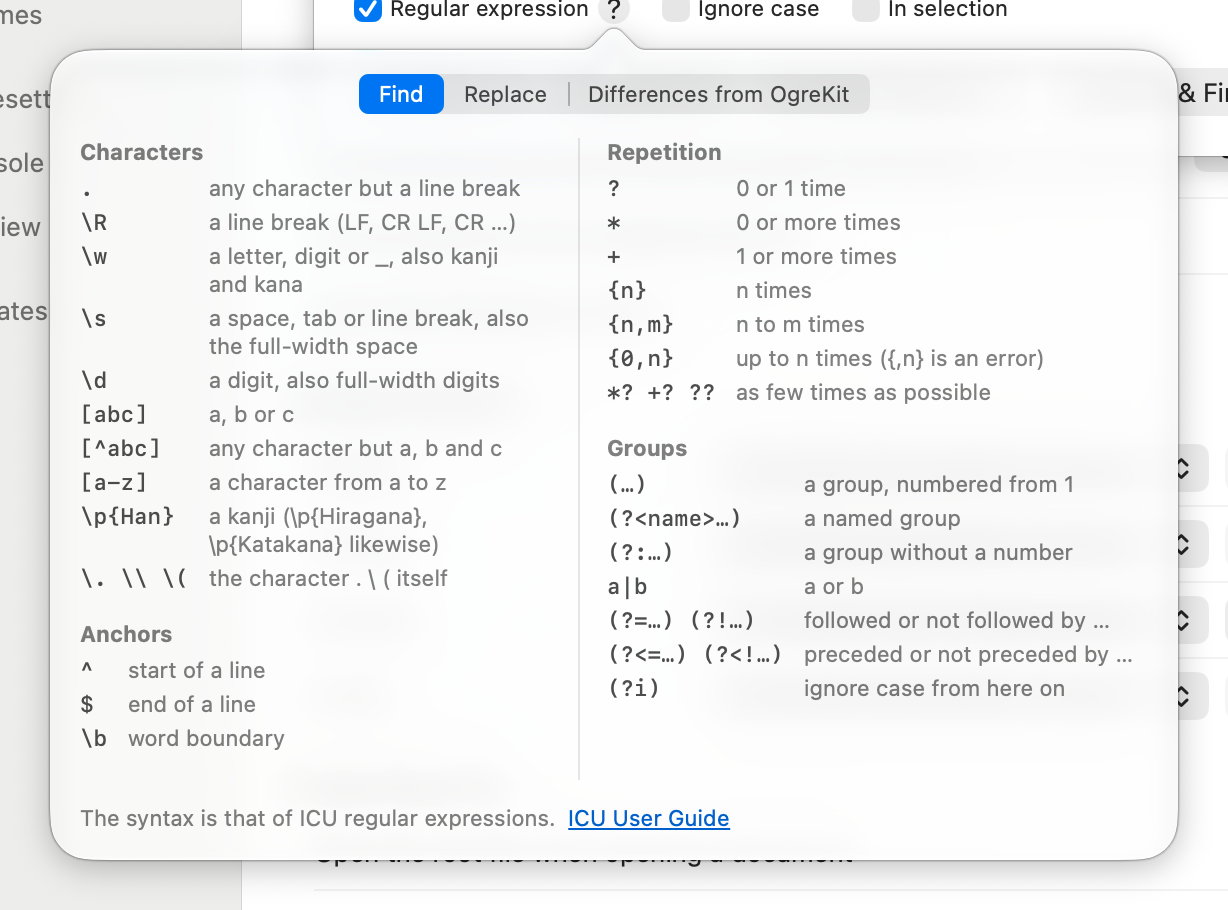
\includegraphics[width=3.6in]{Graphics/manual-regex-reference.png}
\caption{The Regular Expression Reference}
\label{fig:RegexReference}
\end{figure}

The small \mnu{?} button next to \mnu{Regular expression} opens the \mnu{Regular Expression Reference} (\cref{fig:RegexReference}). Its tabs show the syntax of a find pattern (\mnu{Find}), the syntax of a replacement in the style chosen among the options (\mnu{Replace}), and the \mnu{Differences from OgreKit}; the link \mnu{ICU User Guide} at the bottom opens the full description on the web. Dragged away from the panel, the reference stays open as a window of its own.

Some examples:
\begin{itemize}
\item To change \verb|\section{Intro}| into \verb|\section*{Intro}|, search for
\begin{verbatim}
     \\section\{([^}]*)\}
\end{verbatim}
and replace with \verb|\\section*{$1}|.
\item To change every \verb|\label{sec:name}| and \verb|\label{eq:name}| into \verb|\label{sec-name}| and \verb|\label{eq-name}|, search for \verb+\\label\{(sec|eq):([^}]*)\}+ and replace with \verb|\\label{$1-$2}|, as in \cref{fig:AdvancedFind}.
\item To find every character that is not ASCII, search for \verb|[^[:ascii:]]|, then click \mnu{Find All} or choose \mnu{Highlight All}.
\end{itemize}

\section{Multiple Replace}\label{MultipleReplaceSection}

Multiple Replace applies a list of find and replace pairs, called rules, in order from the top, in one step. Use it for replacements you make again and again, such as bringing old commands up to date or converting characters. The lists are kept as sets with names, and each set can be applied to the source in front, to the selection, or to all the files of a document (\cref{TeXRootSearchSection}). Multiple Replace is in the \mnu{Find} submenu with every find interface.

\subsection{The Multiple Replace Window}

\begin{figure}[htbp]
\centering
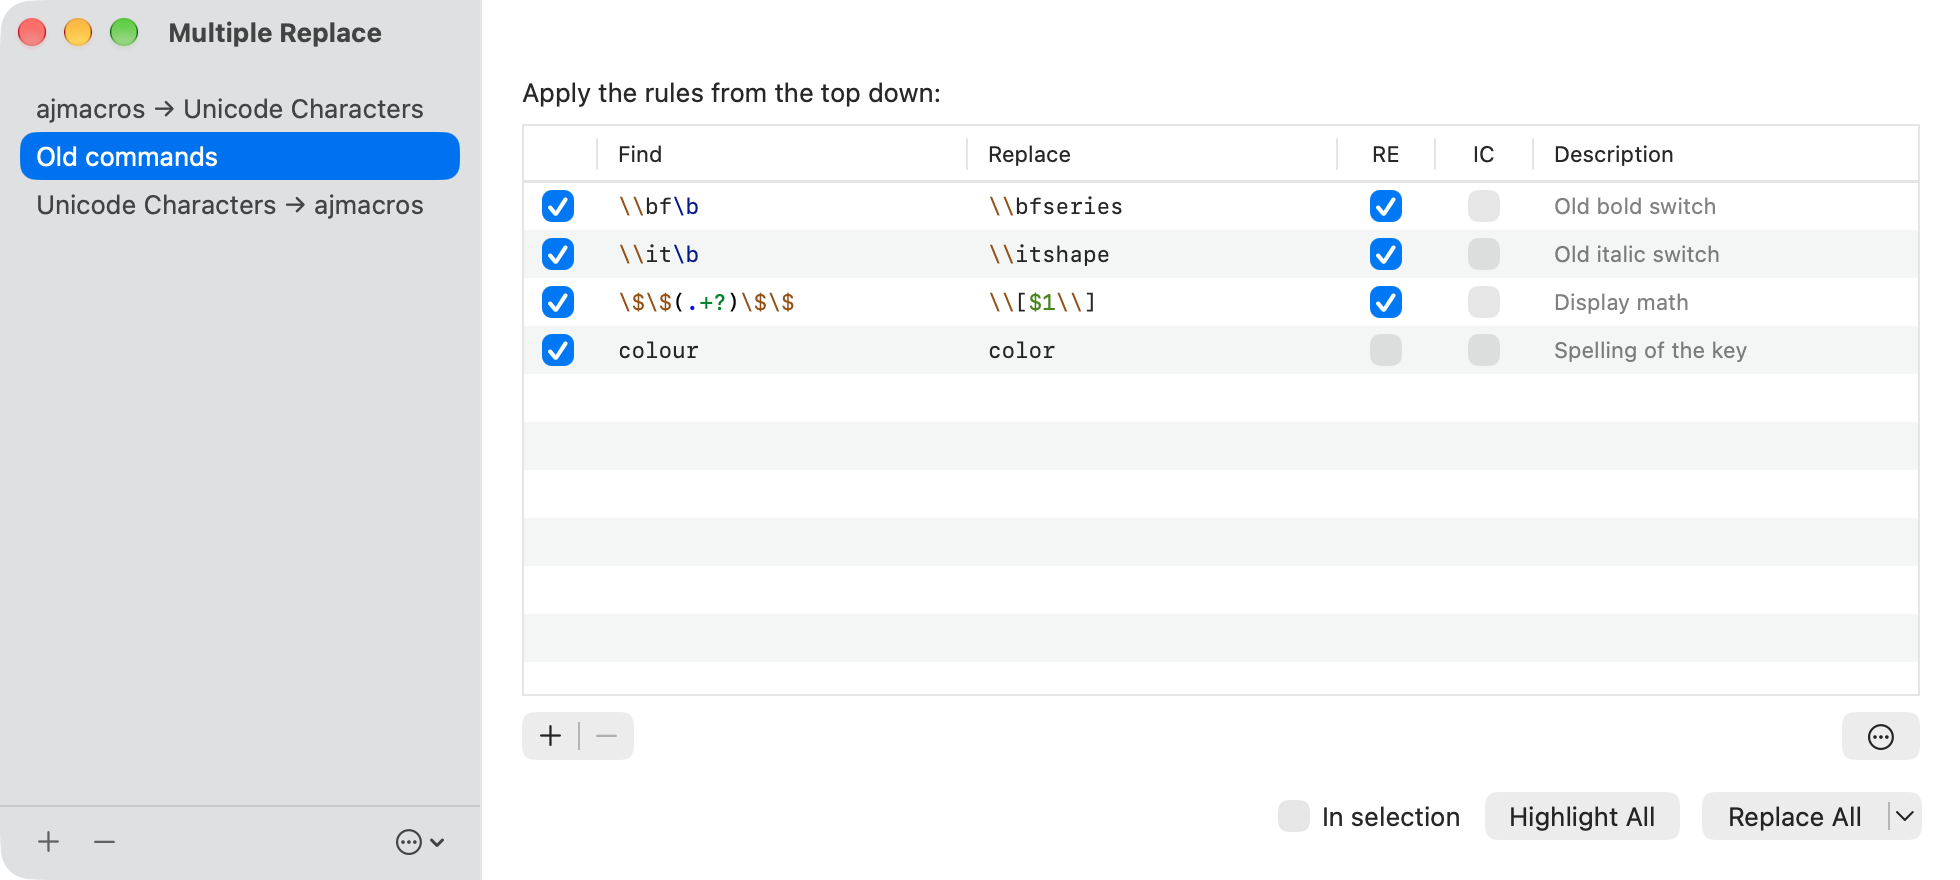
\includegraphics[width=4.7in]{Graphics/manual-multiple-replace.png}
\caption{The Multiple Replace window}
\label{fig:MultipleReplace}
\end{figure}

\mnu{Edit Multiple Replace\ldots} in the \mnu{Find} submenu, or the \mnu{Multiple Replace\ldots} button of the Advanced Find Panel, opens the window (\cref{fig:MultipleReplace}). The sets are listed in the sidebar on the left, and the rules of the selected set on the right. \mnu{Edit Multiple Replace\ldots} has no keyboard shortcut; one can be assigned in the \mnu{Keyboard} category of TeXShop Settings.

Each rule is a row of the table:
\begin{description}
\item[The check box] at the left turns the rule off without removing it.
\item[\mnu{Find} and \mnu{Replace}] are the find and replacement strings. They are colored as in the fields of the panel.
\item[\mnu{RE} and \mnu{IC}] choose a regular expression and ignoring case for this rule alone.
\item[\mnu{Description}] is a note for yourself.
\end{description}
The + and $-$ buttons below the table add a rule and remove the selected rules; drag rules to change their order. The button with three dots at the right below the table shows the \mnu{Options for This Set}, which apply to all its rules, including the replacement syntax. A rule that cannot be used, such as one with an empty or invalid find string, shows a warning sign at the end of its find string; holding the pointer over it explains why. Such a rule is skipped.

Every change in the window is saved at once.

\subsection{Applying a Set}

At the bottom right of the window:
\begin{description}
\item[\mnu{Replace All}] applies the rules of the selected set to the source window in front, or to its selection when \mnu{In selection} is on. A single Undo takes it back, and the line below the table says how many replacements were made. The arrow at the right of the button opens a menu with \mnu{Apply to TeX Sources with the Same TEX root\ldots}, which applies the set to all the files of the document (\cref{TeXRootSearchSection}).
\item[\mnu{Highlight All}] marks what the rules find, without changing anything.
\end{description}
To apply a set without opening the window, choose it in the submenu \mnu{Multiple Replace} of the \mnu{Find} submenu, which lists all the sets. It applies the set to the whole text of the source window in front.

\subsection{Managing Sets}

Below the list of sets:
\begin{itemize}
\item The + button makes a new, empty set.
\item The $-$ button moves the selected set to the Trash.
\item The menu with three dots has \mnu{Duplicate}, \mnu{Import\ldots}, \mnu{Export\ldots} and \mnu{Show in Finder}.
\end{itemize}
To rename a set, click its name in the list when it is selected, and type the new name.

Each set is a file in \path{~/Library/TeXShop/MultipleReplace}: a replacement definition in the JSON format of CotEditor, with the extension \texttt{.json}. \mnu{Show in Finder} opens this folder. \mnu{Import\ldots} reads replacement definitions of CotEditor (\texttt{.cotrpl} or \texttt{.json}) and tab-separated text with one rule per line, so that lists made in other applications can be used. \mnu{Export\ldots} saves the selected set as a file to give to others.

\subsection{Sample Sets}

TeXShop comes with two sample sets, \mnu{Unicode Characters \(\to\) ajmacros} and \mnu{ajmacros \(\to\) Unicode Characters}, named in the language of TeXShop. They convert between Unicode characters and the commands of the \texttt{ajmacros} package, with the same results as the items of the same names in \mnu{Edit}\To\mnu{Character Type Conversion} (\cref{CharacterConversionSection}). The samples are written only when the folder \texttt{MultipleReplace} does not exist yet, so a sample that was changed or removed is not written again; to get them back, move the folder elsewhere and restart TeXShop.

\section{Finding in All Files of a Project}\label{TeXRootSearchSection}

A long document is often split into a root file and chapter files (\cref{chap:projects}). The Find in TeX Sources window finds and replaces in all these files at once: for example, to rename a label used in several chapters, to see every place where a command is used, or to apply a Multiple Replace set to the whole book. Files that are not open are searched and changed too.

\subsection{Which Files Belong to the Project}

TeXShop knows the files of a project by the root line (\cref{sec:root-line}). A chapter file names its root file in a line such as
\begin{verbatim}
     % !TEX root = ../fourier.tex
\end{verbatim}
among its first 20 lines; this root file is its TEX root. The window searches
\begin{itemize}
\item the root file, and
\item the \texttt{.tex} files in the folder of the root file and in the folders below it that name it as their TEX root in such a line (also written \verb|%!TEX root|, without the space).
\end{itemize}
The window does not follow \verb|\input| or \verb|\include|: a chapter file is found by its root line, not by the command that includes it. A file without a root line belongs only to itself. Symbolic links, folders reached through symbolic links or aliases, and the folder \texttt{TeXShop Backups} are left out. When the hidden setting \texttt{UseOldHeadingCommands} is on, files that name the root file with \verb|%SourceDoc| are searched as well (\cref{chap:hidden-settings}).

\subsection{An Example}

Suppose a short book on Fourier series is kept in these files:
\begin{verbatim}
     fourier.tex
     chapters/waves.tex
     chapters/coefficients.tex
     chapters/convergence.tex
     appendix/proofs.tex
\end{verbatim}
\verb|fourier.tex| has the preamble and \verb|\input|s the other files, and each of the other four files starts with \verb|% !TEX root = ../fourier.tex|. The equation of the Fourier series is labeled \verb|eq:series| in \verb|waves.tex| and referred to in the other chapters, and you want to call it \verb|eq:fourier| instead.

\begin{figure}[htbp]
\centering
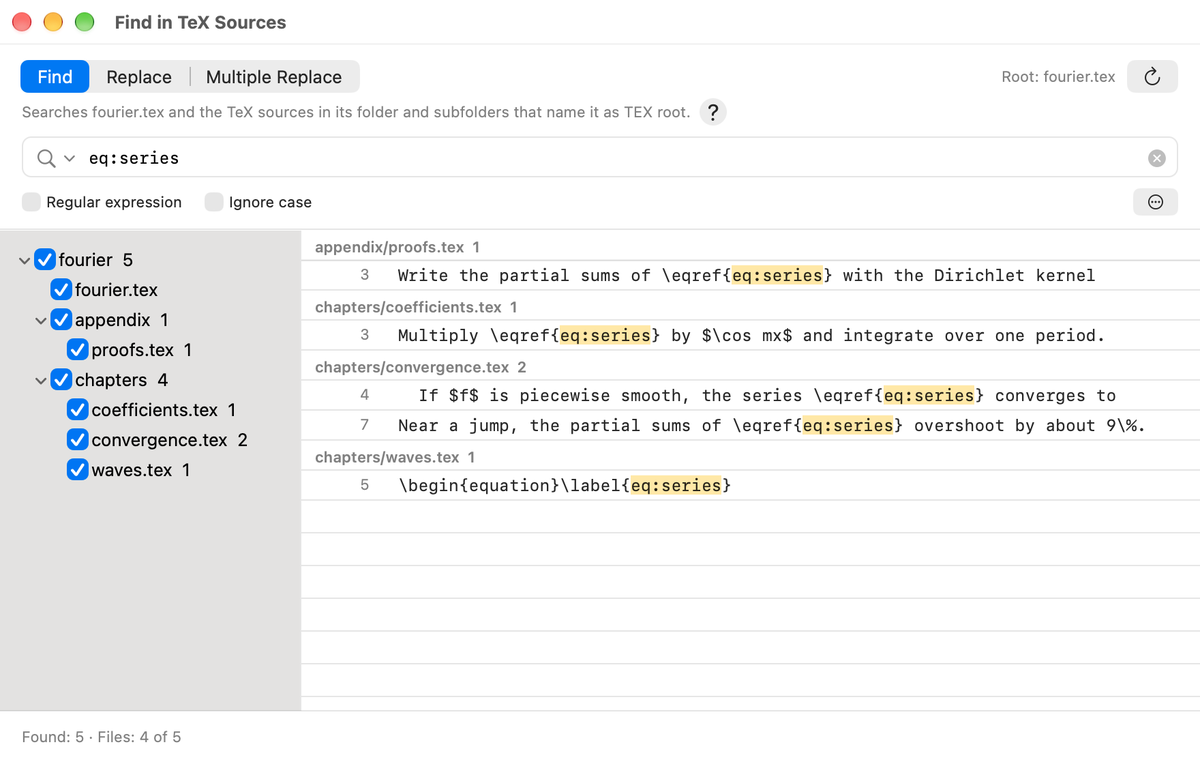
\includegraphics[width=4.7in]{Graphics/manual-texroot-find.png}
\caption{Find in TeX Sources: one label in all the files of a book}
\label{fig:TeXRootSearch}
\end{figure}

\begin{enumerate}
\item Open any of the files, for example \verb|waves.tex|, and choose \mnu{Edit}\To\mnu{Find}\To\mnu{Find in TeX Sources with the Same TEX root\ldots}.
\item In the window, type \verb|eq:series| in the find field. The window lists 5 matches in 4 files (\cref{fig:TeXRootSearch}). On the left are the files of the book in their folders, each with the number of its matches; on the right are the matching lines of each file.
\item Click \mnu{Replace} at the top, and type \verb|eq:fourier| in the replacement field. Each line now appears before and after the replacement, with a check box (\cref{fig:TeXRootReplace}).
\item Turn off the check box of any match that must stay as it is, and click \mnu{Replace All}. After you confirm, all the files are changed.
\end{enumerate}

\begin{figure}[htbp]
\centering
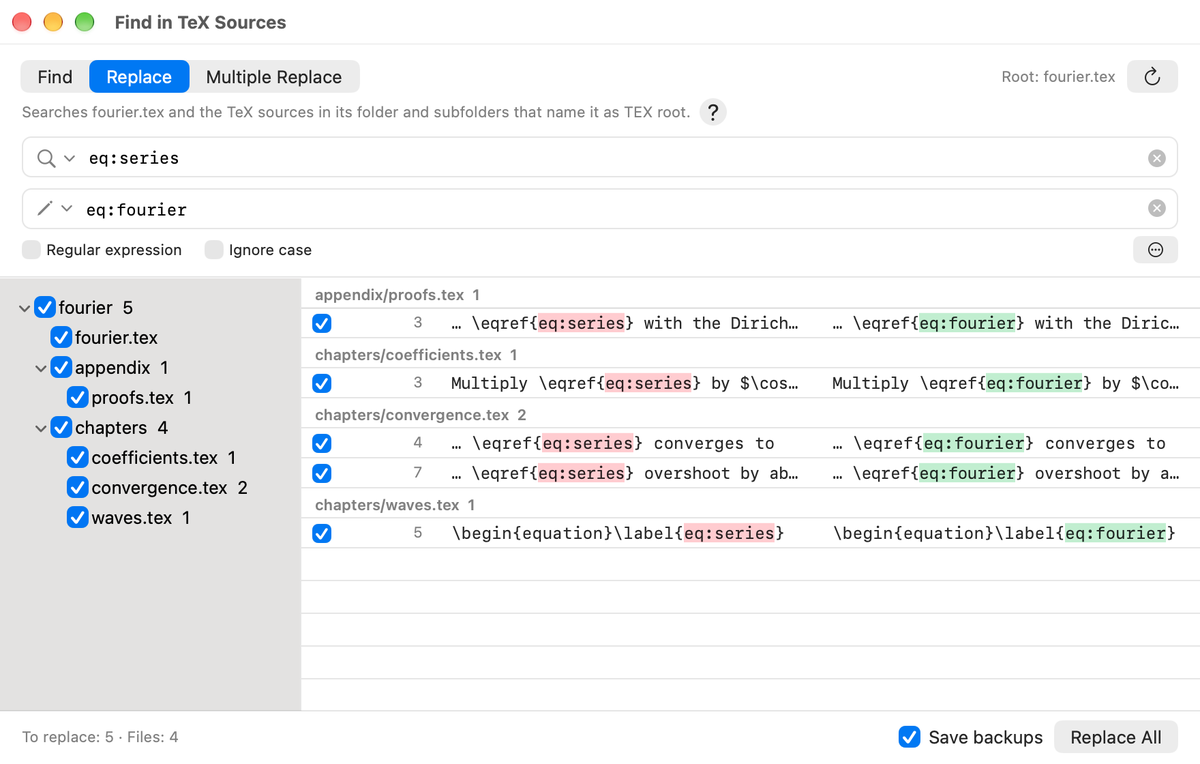
\includegraphics[width=4.7in]{Graphics/manual-texroot-replace.png}
\caption{The Replace mode of Find in TeX Sources}
\label{fig:TeXRootReplace}
\end{figure}

\subsection{Opening the Window}

The window can be opened from three places:
\begin{itemize}
\item \mnu{Edit}\To\mnu{Find}\To\mnu{Find in TeX Sources with the Same TEX root\ldots}. When the file in front has no root line, and so is a root file itself, the item reads \mnu{Find in TeX Sources with This File as TEX root\ldots}; the window then searches this file and the files that name it as their TEX root.
\item The menu of the \mnu{Find All} button of the Advanced Find Panel, with the same item.
\item The menu of the \mnu{Replace All} button of the Multiple Replace window: \mnu{Apply to TeX Sources with the Same TEX root\ldots} (or \mnu{Apply to TeX Sources with This File as TEX root\ldots}) opens the window in the Multiple Replace mode with the set chosen there.
\end{itemize}
The items are dimmed for an untitled document and for a file whose name does not end in \texttt{.tex}. They are in the \mnu{Find} submenu with every find interface.

\subsection{The Window}

From the top, the window (\cref{fig:TeXRootSearch}) has:
\begin{itemize}
\item The modes \mnu{Find}, \mnu{Replace} and \mnu{Multiple Replace}. At the right, \mnu{Root:} names the root file, and the button with a circular arrow (\cmdkey-R) collects the files again, for example after you have added a chapter file.
\item A line that says which files are searched. Its \mnu{?} button explains the rule and has a button to open TeXShop Help.
\item The find field and, in the Replace mode, the replacement field, with \mnu{Regular expression}, \mnu{Ignore case} and the button with three dots for more options. These are the fields and options of the Advanced Find Panel: what you type in one shows in the other.
\item On the left, the files and folders with the number of matches. Turn off a file or a folder to leave it out.
\item On the right, the matches, grouped by file.
\item At the bottom, the number of matches and of files. The stop button, the Escape key or \cmdkey-. stops a long search. If some files or folders could not be read, the button \mnu{Files not read} lists them with the reason.
\end{itemize}

Click a row to show the match in its document, opening the file if needed; double-click it to bring that window to the front. With the keyboard, Return shows the selected match and Space turns its check box on or off. The list follows your edits in open documents.

An open document is searched as it is on the screen, with its unsaved changes; a file that is not open is read from the disk in the encoding TeXShop would open it in.

\subsection{Replacing in All Files}

The window replaces in three steps: look at the changes, turn off those you do not want, then replace.
\begin{description}
\item[Replace] shows each line before and after the replacement. Every match has a check box; a match turned off is not replaced.
\item[Multiple Replace] applies a set of the Multiple Replace window, chosen in the pop-up menu under the field, and lists the groups of changed lines, each with one check box. \mnu{Edit\ldots} opens the set in the Multiple Replace window. When a long change is shortened to ``\ldots\ more lines'', \mnu{Show All Lines} (\cmdkey-Y) in the contextual menu of the row shows all of it.
\end{description}

\mnu{Replace All} asks before it replaces, and says how many files that are not open will be changed on the disk. With \mnu{Save backups} on, each file to be changed is first copied into the folder \texttt{TeXShop Backups} next to the root file, in a folder named after the date and time.

Files that are not open are then written directly, in their own encoding and with their line endings; this cannot be undone except from the backup. Open documents are changed on the screen and are not saved, and one Undo in a document takes back its replacements. Afterwards the files are searched again, and the line at the bottom says how many matches were replaced.

Some files can only be searched, not replaced in, for example a file that cannot be written or that its encoding cannot save back unchanged. They are marked with $\oslash$, and the mark gives the reason. If some files could not be changed, a sheet lists them with the reason; \mnu{Show in Finder} opens the folder of the backup, and \mnu{Open the Original Text in a New Document} opens the text of a partly changed document as it was before.

Do not run Replace All while another application keeps writing these files.

\section{Other Find Interfaces}\label{FindInterfaceSection}

The pop-up menu \mnu{Find interface}, in the \mnu{Find} group of the \mnu{Editor} category of TeXShop Settings, chooses what \mnu{Find} opens:
\begin{description}
\item[Advanced Find Panel (recommended)] The panel described in this chapter. It is the default.
\item[Apple Find Bar] The find bar of macOS, at the top of the source, as in Safari and Xcode. It looks minimal, but has more features than it first shows.
\item[Apple Find Panel] The basic find panel of macOS.
\item[OgreKit Find Panel (Legacy)] The find panel of the OgreKit project by Isao Sonobe, with regular expressions of its own. It remains available as a legacy choice.
\end{description}
Switching among the Apple Find Panel, the Apple Find Bar and the Advanced Find Panel takes effect immediately. Switching to or from the OgreKit Find Panel requires restarting TeXShop.

With the other interfaces, the commands of the panel, such as \mnu{Find All} and \mnu{Highlight All}, are not in the \mnu{Find} submenu. Multiple Replace and Find in TeX Sources stay there and work as described above.

% ===== 14-macros.tex
\chapter{Macros}\label{MacrosChapter}

Macros are listed in the \mnu{Macros} menu and in the \mnu{Macros} pop-up menu of the source window's toolbar. There are two kinds. \emph{Text macros} insert text into the source, like the buttons of the LaTeX Panel. \emph{AppleScript macros} run a script in AppleScript, the scripting language of macOS, which can control TeXShop and other applications: they can typeset, run programs in a shell, ask questions in dialogs and change the source. Macros are changed, added and arranged in the Macro Editor.

\section{The Default Macros}\label{DefaultMacrosSection}

The best way to understand the macros that come with TeXShop is to look at them in the Macro Editor (\mnu{Macros}\To\mnu{Open Macro Editor\ldots}): select a macro in the list, and its contents appear beside it. Among them:
\begin{description}
\item[Program, Encoding, Root] write a magic comment line at the top of the source, replacing a similar line that is already there. \mnu{Program} lists the engines and writes, for example, \verb|% !TEX TS-program = xelatex|, the older form of the program line, which TeXShop reads in the same way (\cref{MagicCommentsChapter}); it replaces a \verb|TS-program| line but not a \verb|% !TEX program| line, so delete such a line yourself. \mnu{Encoding} chooses an encoding and \mnu{Root} the root file of a project. Magic comment lines are particular about spaces and capitalization, and these macros take care of that. \mnu{Root (Short Version)}, \mnu{Numbering} and the \mnu{Special Comments} submenu insert other magic comment lines as text.
\item[Insert Begin/End] Type the name of an environment, such as \texttt{theorem}, select it and choose this macro. The word is replaced with
\begin{verbatim}
     \begin{theorem}

     \end{theorem}
\end{verbatim}
and the insertion point is placed on the line between. \mnu{Close Begin/End} adds the \verb|\end| line of the environment that is open.
\item[Insert reference] searches the current file for \texttt{\textbackslash label} commands and lets you choose a label from a list; it inserts the label wrapped in \texttt{\textbackslash ref\{\ldots\}}, a command you can change in the script. If text is selected, only the labels that contain it are listed. \mnu{Goto label} goes to a label chosen from a similar list.
\item[Open quickly\ldots] lists the \texttt{.tex}, \texttt{.sty} and \texttt{.pdf} files in the folder of the current source file and opens the ones you choose.
\item[Column macros] \mnu{New tabular} and \mnu{New array} insert a \texttt{tabular} or \texttt{array} environment with the numbers of rows and columns you enter, and \mnu{Add column} and \mnu{Delete column} change the rows you select.
\item[Paste Spreadsheet Cells] pastes cells copied from Excel or another spreadsheet application into the source as a table. It asks for a table style: \texttt{cells} converts the copied text to table cells only; \texttt{simple} puts a simple \texttt{tabular} environment around them; \texttt{booktabs} takes the first line as a header and places \verb|\toprule|, \verb|\midrule| and \verb|\bottomrule| in a \texttt{tabular} environment; \texttt{longtable} takes the first line as a header and puts the cells in a \texttt{longtable} environment with its header lines. The macro replaces the contents of the clipboard with the \LaTeX\ text, so to paste the same cells in another style, copy them again in the spreadsheet first.
\item[Applescript] This submenu opens the PDF of the document in Preview or Adobe Acrobat, shows the source and PDF files in the Finder, opens the home pages of TeXShop and MacTeX, and opens a file of the \TeX\ Live tree by its name (\mnu{View TeX Live file}). \mnu{Convert to MAC}, \mnu{Convert to Unix} and \mnu{Convert to Windows} write a copy of the saved source with the line endings of very old Macintosh files (a carriage return), of macOS and Unix (a line feed) or of Windows (a carriage return and a line feed); for \texttt{MyFile.tex} the copy is \texttt{MyFile\_Mac.tex}, \texttt{MyFile\_Unix.tex} or \texttt{MyFile\_Windows.tex}. TeXShop itself reads all three kinds of line endings; the copies are for other editors that cannot. \mnu{Bibliography} runs \LaTeX, Bib\TeX, \LaTeX\ and \LaTeX\ one after another (\cref{TypesettingScriptSection}).
\item[Claus Gerhardt Macros] These macros run shell scripts in \path{~/Library/TeXShop/bin}, most of them of the same names, and work on a saved file. \mnu{htlatexc} runs \cmd{htlatex} to make a web page of the document and opens it in Safari; \mnu{htlatexr} does the same with the option \texttt{-r}, which makes the images again even when they exist. \mnu{pdfselectc} makes PDF files with selected pages of the document's PDF: it asks how many files to make and then for the pages of each, such as \texttt{5:8} for pages 5 to 8. \mnu{mpostc} runs MetaPost and then pdf\LaTeX; \mnu{mpostcpl} runs pdf\LaTeX, MetaPost and pdf\LaTeX\ again; \mnu{latex-makeindex-mpost} runs pdf\LaTeX, MakeIndex, MetaPost and pdf\LaTeX. \mnu{pdflatexc} is explained in \cref{ShellScriptSection}.
\end{description}
The other macros, from \mnu{Headings} to \mnu{Figures}, are text macros that insert document headings, sectioning commands, mathematical environments, text styles, lists, footnotes and similar \LaTeX\ constructions.

\section{Where Macros Are Kept}\label{MacroFilesSection}

The macros are stored in
\begin{verbatim}
     ~/Library/TeXShop/Macros/Macros_Latex.plist
\end{verbatim}
and the Macros menu shows them for every typesetting engine. A separate set can be kept for the built-in commands plain \TeX, Bib\TeX, MakeIndex and MetaPost: when one of these is chosen for the document, the Macro Editor saves its macros in a file of its own, such as \texttt{Macros\_Tex.plist}, and leaves \texttt{Macros\_Latex.plist} unchanged.

If the \texttt{Macros} folder is missing when TeXShop starts, TeXShop creates it again with the default macros. If \texttt{Macros\_Latex.plist} is damaged, TeXShop replaces it with its own copy when it starts and keeps the damaged file in \path{~/Library/TeXShop/Backups}. To start over with the default macros, quit TeXShop, move the \texttt{Macros} folder to the desktop and start TeXShop again; the moved folder keeps your old macros.

\section{The Macro Editor}\label{MacroEditorSection}

Choose \mnu{Macros}\To\mnu{Open Macro Editor\ldots} (\cref{fig:MacroEditor}). The list on the left shows the Macros menu as an outline, like the list view of a Finder window, with the shortcut of each macro at the right; the contents of the selected macro appear on the right and can be edited there. The contents are shown in the console font; \mnu{Use Also for Macro Editor} in the \mnu{Console} category of TeXShop Settings decides this.

\begin{figure}[htbp]
\centering
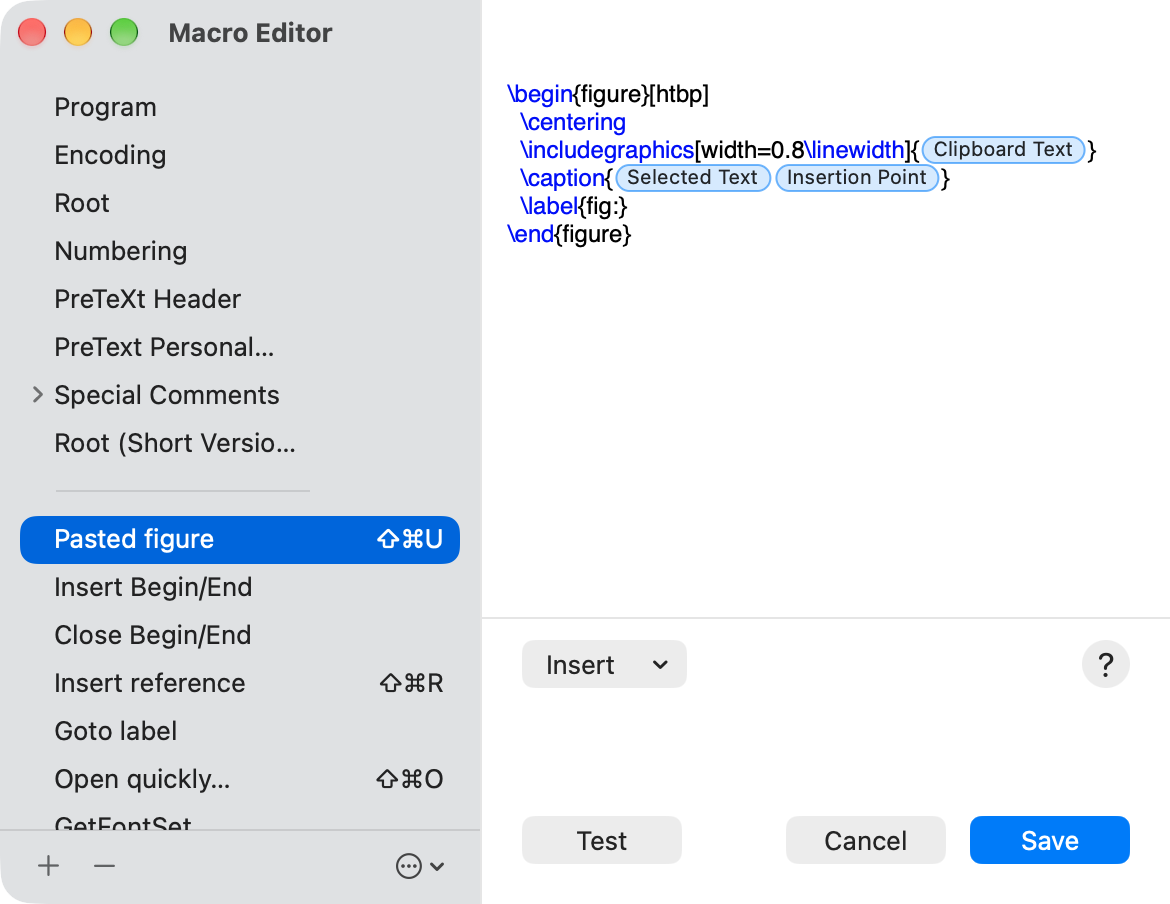
\includegraphics[width=4.5in]{Graphics/manual-macro-editor.png}
\caption{The Macro Editor, with the contents of a text macro and its shortcut in the list}
\label{fig:MacroEditor}
\end{figure}

Changes made in the Macro Editor take effect when you click \mnu{Save}, which updates the Macros menu and the file of the macros. \mnu{Cancel} closes the Macro Editor without the changes; if you close its window with unsaved changes, TeXShop asks whether to save them. \mnu{Test} runs the selected macro, as it now stands in the editor, in the active document, so that you can try it before saving; double-clicking a macro in the list does the same.

\begin{description}
\item[Adding and deleting] Click + below the list to add an item. The menu at the right end of the bar below the list adds a submenu or a separator and duplicates the selected items; $-$ deletes them. A new item or submenu is named at once: type its name and press Return. Submenus can be nested to any level.
\item[Rearranging] Drag an item to another place; drag it left or right to place it at another level, inside or outside a submenu.
\item[Renaming] Select an item and press Return, or click its name once more after a moment, as in the Finder. Type the new name and press Return; Escape keeps the old name.
\item[Shortcuts] Select an item and click its shortcut in the list, or double-click the shortcut, then press the new shortcut: Command or Control with a key, or one of F1--F20, with Shift and Option as needed. If a menu command or another macro already uses the shortcut, TeXShop says so below the contents and does not change it; press another shortcut. To remove a shortcut, click \mnu{Remove Shortcut} ($\ominus$) in the field or press Delete; Escape keeps the one it had. A shortcut that is inactive because a menu command or an earlier macro uses it is marked with a warning triangle in the list; select the item to see the reason below the contents. \Cref{MacroShortcutsSection} explains how menu and macro shortcuts work together.
\item[Placeholders] In the contents, the placeholders that a macro replaces, described below, are shown as rounded tokens that say what they stand for, such as \mnu{Selected Text}. The macro keeps them as they are written, so copying and saving work as usual. Type a placeholder, or choose it from the \mnu{Insert} menu below the contents; the help button at its right lists them all. Deleting next to a token deletes all of it.
\item[Sharing macros] While the Macro Editor is open, the Macros menu has two more commands. \mnu{Save selection to file\ldots} saves the selected macros in a file of their own, which you can give to others. \mnu{Add macros from file\ldots} adds the macros of such a file to your list; then arrange them in the Macro Editor as you like.
\end{description}

\section{Text Macros}\label{TextMacrosSection}

The text of a text macro is inserted into the source, with these replacements:
\begin{description}
\item[\texttt{\#SEL\#}] is replaced with the text that was selected when the macro was chosen, or with nothing if no text was selected.
\item[\texttt{\#INS\#}] marks where the insertion point goes. Without it, the insertion point is placed at the end of the inserted text.
\item[\texttt{\#PASTE\#}] is replaced with the text on the clipboard, or with nothing if the clipboard holds no text.
\item[\texttt{•}] is a mark, which \mnu{Edit}\To\mnu{Marks} can move to (\cref{MarksSection}).
\end{description}
For example, a text macro that puts a selected word into an environment of that name reads
\begin{verbatim}
     \begin{#SEL#}
     #INS#
     \end{#SEL#}
\end{verbatim}

\subsection{Macros for Dropped Files}\label{DragAndDropMacros}

When a file is dragged from the Finder onto the source, TeXShop inserts a command for it (\cref{DragAndDropSection}). To insert something else for a kind of file, add a submenu named \mnu{Drag \& Drop} at the top level of the Macros menu. In it, add an item named after the extension, such as \mnu{.pdf}, whose content is the text to insert, for example \verb|\includegraphics[#INS#]{%r}|; an item named \mnu{.*} is used for the other extensions, those that have neither an item of their own nor a command of their own in the table of \cref{DragAndDropSection}. The content can use these abbreviations:
\begin{center}
\begin{tabular}{ll}
\verb|%F| & the full path of the dropped file \\
\verb|%f| & the name of the file \\
\verb|%r| & the path of the file from the folder of the source file \\
\verb|%n| & the name of the file without its extension \\
\verb|%e| & the extension \\
\end{tabular}
\end{center}

\section{AppleScript Macros}\label{AppleScriptMacrosSection}

A macro whose contents begin with
\begin{verbatim}
     --AppleScript
\end{verbatim}
or
\begin{verbatim}
     --AppleScript direct
\end{verbatim}
runs as an AppleScript when it is chosen; the case of the letters does not matter, and a space may follow the two hyphens. For example, \mnu{Macros}\To\mnu{Applescript}\To\mnu{View pdf with Preview} opens the PDF of the active document in Preview, once the PDF has been typeset. Its contents are
\begin{verbatim}
     --AppleScript direct

     tell application "Preview"
       activate
       open POSIX file #PDFPATH#
     end tell
\end{verbatim}

A script beginning with \verb|--AppleScript direct| is run by TeXShop itself. While it runs, TeXShop does not respond to anything else, so the script cannot ask TeXShop to do something that might need your input. For example, it cannot ask TeXShop to run \LaTeX: if the file had an error, the console would wait for your input, which TeXShop could not receive. If such a script ends with a text as its result, TeXShop shows the text in an alert.

A script beginning with \verb|--AppleScript| is run by ScriptRunner, a small program inside TeXShop. Such a script can ask TeXShop to do things that might need your input, because ScriptRunner waits while TeXShop stays active. So \verb|--AppleScript direct| suits simple macros, while \verb|--AppleScript| is needed for scripts that typeset or otherwise work with TeXShop.

AppleScript is a language of its own; Apple's \emph{AppleScript Language Guide}, on Apple's developer website, describes it in full. The document \mnu{Help}\To\mnu{Older Documents}\To\mnu{Notes on Applescript in TeXShop} explains in depth how scripts work with TeXShop.

\subsection{Paths and the Document Name}

Before running an AppleScript macro, TeXShop replaces the following strings with the path of a file of the active document, in double quotes:

\begin{description}
\item[\texttt{\#FILEPATH\#}] the source file
\item[\texttt{\#TEXPATH\#}] the source file with the extension \texttt{.tex}
\item[\texttt{\#NAMEPATH\#}] the source file without its extension
\item[\texttt{\#FOLDERPATH\#}] the folder that contains the source, ending with a slash
\item[\texttt{\#PDFPATH\#}, \texttt{\#DVIPATH\#}, \texttt{\#PSPATH\#}] the \texttt{.pdf}, \texttt{.dvi} and \texttt{.ps} files
\item[\texttt{\#LOGPATH\#}, \texttt{\#AUXPATH\#}] the \texttt{.log} and \texttt{.aux} files
\item[\texttt{\#INDPATH\#}, \texttt{\#BBLPATH\#}, \texttt{\#HTMLPATH\#}] the \texttt{.ind}, \texttt{.bbl} and \texttt{.html} files
\item[\texttt{\#DOCUMENTNAME\#}] the name of the document
\end{description}

For example, if \texttt{\#FILEPATH\#} gives \nolinkurl{/Users/name/Projects/Fourier/Fourier.tex}, \texttt{\#FOLDERPATH\#} gives \nolinkurl{/Users/name/Projects/Fourier/}. If the document has never been saved, \texttt{\#FILEPATH\#} is an empty string.

\texttt{\#DOCUMENTNAME\#} is the name of the document as the title of the source window shows it: with its extension, or without it if the extension is hidden. A script uses it to address the document that called it:
\begin{verbatim}
     tell document #DOCUMENTNAME# of application "TeXShop"
       latex
     end tell
\end{verbatim}

\subsection{TeXShop's AppleScript Commands}

An AppleScript can do its work in two ways: it can call TeXShop's own commands, or it can run shell commands. TeXShop understands these commands:

\begin{description}
\item[\texttt{typeset}, \texttt{latex}, \texttt{tex}, \texttt{bibtex}, \texttt{makeindex}, \texttt{metapost}] typeset continuously, without stopping at errors.
\item[\texttt{typesetinteractive}, \ldots] \texttt{typesetinteractive}, \texttt{latexinteractive}, \texttt{texinteractive}, \texttt{bibtexinteractive}, \texttt{makeindexinteractive} and \texttt{metapostinteractive} typeset too, but stop at an error so that you can answer in the console.
\item[\texttt{taskdone}] returns NO while typesetting is still running, and YES when it is done.
\item[\texttt{refreshpdf}, \texttt{refreshtext}] make the PDF and the source show the latest version of their files on the screen.
\item[\texttt{goto line}] selects a line in the source.
\end{description}

A typesetting command returns at once, before typesetting is finished; use \texttt{taskdone} to wait for it (\cref{TypesettingScriptSection}). For example, this selects line 37:
\begin{verbatim}
     tell document #DOCUMENTNAME# of application "TeXShop"
       goto line 37
     end tell
\end{verbatim}
A script can also read and change the text and the selection of a document and search in it; the macros \mnu{Program} and \mnu{Insert Begin/End} are examples.

\subsection{Dialogs}

An AppleScript can show dialogs and act on what you enter. For example, make a macro with the following contents and try it:
\begin{verbatim}
     --AppleScript
     activate
     display dialog "Test dialog: type something below" ¬
        default answer "Hello World!" ¬
        buttons {"A", "B", "C"} default button "B"
     set {theText, theButton} to ¬
        {the text returned of the result, ¬
         the button returned of the result}
\end{verbatim}
A dialog can have at most three buttons. The command \texttt{activate} is needed because a macro beginning with \verb|--AppleScript| is run by ScriptRunner, so its dialogs are shown by ScriptRunner rather than by TeXShop; \texttt{activate} brings ScriptRunner to the front, so that the dialogs appear in front of other windows.

\section{Example: A Sequence of Typesetting Commands}\label{TypesettingScriptSection}

A document with a bibliography needs a sequence of typesetting runs: \LaTeX\ writes the \texttt{.aux} file, Bib\TeX\ uses it to write the \texttt{.bbl} and \texttt{.blg} files, \LaTeX\ runs again to add the bibliography to the document, and once more to update the references to it. Your projects may need similar sequences, and an AppleScript macro can run them for you. The macro \mnu{Macros}\To\mnu{Applescript}\To\mnu{Bibliography} shows how:
{\small
\begin{verbatim}
  --Applescript

  set fileName to #FILEPATH#
  if fileName is equal to  ""
  activate
  display dialog "Please save the file first"  buttons {"OK"} default button "OK"
  return
  end if

  set frontName to #DOCUMENTNAME#

  tell document frontName of application "TeXShop"

      latexinteractive

      repeat
          delay 2
          if taskdone
              exit repeat
          end if
      end repeat

      bibtex

      repeat
          delay 2
          if taskdone
              exit repeat
          end if
      end repeat

      latex

      repeat
          delay 2
          if taskdone
              exit repeat
          end if
      end repeat

      latex

      repeat
          delay 2
          if taskdone
              exit repeat
          end if
      end repeat

  end tell
\end{verbatim}
}

The first line makes this an AppleScript macro run by ScriptRunner, so it can ask TeXShop to typeset. The next lines check \texttt{\#FILEPATH\#}, the full path of the source file. It is an empty string when the document has not been saved yet; in that case the script asks you to save it and stops. The script then refers to the document by \texttt{\#DOCUMENTNAME\#}. TeXShop saves the document itself when a typesetting command starts, so the script does not need to save it.

The remaining commands run \texttt{latexinteractive}, \texttt{bibtex}, \texttt{latex} and \texttt{latex}. A typesetting command returns to the script at once, so after each command a \texttt{repeat} loop waits until \texttt{taskdone} reports that the job is complete. The line \texttt{delay 2} makes the script pause between the checks rather than asking continually and slowing down the computer.

\section{Example: Calling a Shell Script}\label{ShellScriptSection}

The macro \mnu{pdflatexc}, in \mnu{Macros}\To\mnu{Claus Gerhardt Macros}, shows how an AppleScript calls a shell script. The shell script itself is simple: it adds the folders of the \TeX\ programs to the search path and runs \cmd{pdflatex} with \texttt{--shell-escape}. Your own scripts will probably do more, for instance run several programs in sequence; that is when these techniques become useful.

The shell script is \path{~/Library/TeXShop/bin/pdflatexc}. It does not depend on TeXShop: if its folder is in your search path, typing \texttt{pdflatexc myfile.tex} in Terminal runs it. Here it is:
\begin{verbatim}
     #!/bin/tcsh
     # pdflatexc
     # Claus Gerhardt
     #
     # Usage
     # pdflatexc filename.tex

     set path= ($path /Library/TeX/texbin /usr/texbin /usr/local/bin)

     pdflatex --shell-escape "$1"
\end{verbatim}

The macro that calls this shell script is more interesting:
{\scriptsize
\begin{verbatim}
--Applescript
-- Apply only to an already saved file.

set scriptPath to (do shell script "dirname " & "~/Library/TeXShop/Scripts/ex")
set scriptPath to scriptPath & "/setname.scpt"
set scriptName to POSIX file scriptPath as alias
set scriptLiB to (load script scriptName)
tell scriptLib
set frontName to setname(#NAMEPATH#,#TEXPATH#)
end tell

set fileName to  #TEXPATH#
set n to (number of characters of contents of fileName)
set fileNamequoted to quoted form of fileName
set baseName to do shell script "basename " & fileNamequoted
set m to (number of characters of contents of baseName)
set dirName to quoted form of (characters 1 thru (n - m - 1) of fileName as string)

set shellScript to "cd " & dirName & ";"
set shellScript to shellScript & "~/Library/TeXShop/bin/pdflatexc  " & quoted form of baseName
do shell script shellScript

tell document frontName of application "TeXShop"
    refreshpdf
end tell
\end{verbatim}
}

After the comments, the first seven lines save the source file and find the name of its document, which is put in \texttt{frontName}. The work is done by the compiled script \texttt{setname.scpt} in \path{~/Library/TeXShop/Scripts}: these lines find its path, load it and call it with \texttt{\#NAMEPATH\#} and \texttt{\#TEXPATH\#}. Often the same can be done more simply with
\begin{verbatim}
     set frontName to #DOCUMENTNAME#
     tell document frontName of application "TeXShop"
         save
     end tell
\end{verbatim}
The longer recipe has two advantages. It also works when the front document is not the one that should receive the later commands, for instance a log file. And if the file has never been saved, it returns an error, while the \texttt{save} command would leave the script waiting behind a save dialog.

The next six lines set the variables \texttt{dirName} and \texttt{baseName}. If the source file is \nolinkurl{/Users/name/My Papers/Stuff/myfile.tex}, \texttt{dirName} is \verb|'/Users/name/My Papers/Stuff'|, quoted for the shell because of the space in a folder name, and \texttt{baseName} is \texttt{myfile.tex}. The file name is quoted the same way when it is passed to the shell script, so both may contain spaces.

The next three lines call the shell script. The result is the same as typing
{\small
\begin{verbatim}
  cd '/Users/name/My Papers/Stuff'; ~/Library/TeXShop/bin/pdflatexc 'myfile.tex'
\end{verbatim}
}
in Terminal. The final three lines update the Preview window. Several of these lines are complicated, but they can be copied unchanged into new scripts.

\subsection{Running Shell Commands from AppleScript}

AppleScript runs a shell command in the form
\begin{verbatim}
     do shell script "cmd input"
\end{verbatim}
To build a command from parts, write it in the equivalent form
\begin{verbatim}
     do shell script "cmd " & "input"
\end{verbatim}
Notice the space after \texttt{cmd}: the ampersand joins two strings, so \verb|"cmd " & "input"| is \verb|"cmd input"|.

A shell started by AppleScript begins in the root folder, and each \texttt{do shell script} starts a new shell, so a later command would not be in the folder that an earlier \texttt{cd} chose. To run further commands in the same folder, join them with semicolons into one command, as in Terminal:
\begin{verbatim}
     do shell script "cmd1 " & "input1" & ";" & "cmd2 " & "input2"
\end{verbatim}
The macro above does this with \texttt{cmd1} = \texttt{cd}, \texttt{input1} = \texttt{dirName}, which is already quoted, \texttt{cmd2} = \path{~/Library/TeXShop/bin/pdflatexc} and \texttt{input2} = \texttt{baseName}; it collects them in the variable \texttt{shellScript} for convenience.

% ===== 15-keyboard.tex
\chapter{Keyboard Shortcuts}\label{KeyboardChapter}

Any menu command of TeXShop can be given a shortcut of your choice, or have its shortcut removed, in the \mnu{Keyboard} category of TeXShop Settings. Shortcuts of macros are set in the Macro Editor (\cref{MacroEditorSection}). Key bindings, which make a single typed character insert text, and the trigger key of command completion are described in \cref{KeyBindingsSection,CommandCompletionSection}.

\section{Changing Menu Shortcuts}\label{Define_Shortcut}\label{sec:MenuShortcutKeystrokes}

Choose \mnu{TeXShop}\To\mnu{Settings\ldots} and select \mnu{Keyboard}. The \mnu{Menu Shortcuts} group (\cref{fig:MenuShortcuts}) lists the menu commands, by their menu paths, with their shortcuts. Select a command and click its shortcut, double-click the command, or press Return; then press the new shortcut. Escape or Return keeps the old one, and Tab moves on. A shortcut must use the Command or Control key, or be one of the function keys F1--F20; Shift and Option may be added. If another command already uses the shortcut, TeXShop says so below the list and does not change anything; press another shortcut. To remove a shortcut, click \mnu{Remove Shortcut} ($\ominus$) in the field or press Delete.

Changes take effect immediately and are kept when TeXShop restarts; they do not depend on the language of the menus. The line below the list shows the default shortcut of the selected command. \mnu{Restore Default} gives the selected command its default shortcut back, and \mnu{Restore All\ldots} does this for all commands.

\begin{figure}[htbp]
\centering
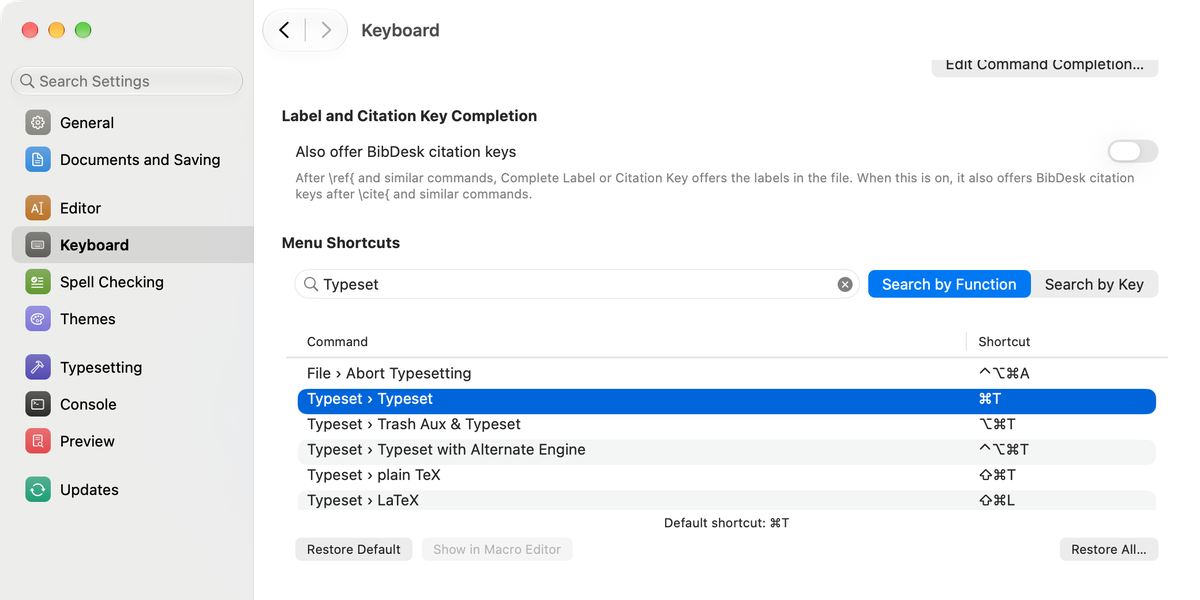
\includegraphics[width=4.5in]{Graphics/manual-menu-shortcuts.png}
\caption{Menu Shortcuts in the Keyboard category of Settings, searching by function}
\label{fig:MenuShortcuts}
\end{figure}

The list also has the commands that appear only while the Option key is held down, such as \mnu{Trash Aux \& Typeset}, and the commands that TeXShop adds to its menus, such as those of the Advanced Find Panel. When \mnu{Enable Autosave and Versions} is on in the \mnu{Documents and Saving} category, macOS adds \mnu{Duplicate} and \mnu{Close All} to the File menu; their shortcuts can be changed like those of other commands. A command whose shortcut macOS sets, such as \mnu{Save As\ldots} while autosave is on, is dimmed in the list and marked \mnu{Shortcut Unavailable}.

\section{Finding a Command or a Key}\label{ShortcutSearchSection}

Two modes above the list help to find what you want to change:
\begin{description}
\item[Search by Function] finds a command by its name or by its menu path: type a word in the search field. A menu command found with \mnu{Search Settings}, at the top of the sidebar of Settings (\cref{sec:SearchSettings}), opens \mnu{Keyboard} with the command in this field.
\item[Search by Key] finds what a key does: click \mnu{Search by Key} and press a shortcut, and the list shows the menu commands and macros that use it, which one is in effect and why the others are inactive. Press Escape to stop. For a macro, choose \mnu{Show in Macro Editor} to edit it there. The trigger key of command completion, alone or with Shift, Option or Control, is reported as reserved for command completion.
\end{description}

\section{Menu Shortcuts and Macro Shortcuts}\label{MacroShortcutsSection}

Menu commands and macros can use the same keys. For the same key and modifiers, a menu command takes precedence over a macro, with its customized shortcut when it has one; a macro can use a key that a menu command no longer has. Among macros, the first one in the Macros menu with the key takes it.

Giving a menu command a shortcut that a macro uses, or restoring such a default, asks for confirmation; the macro stays in the Macros menu, but its shortcut becomes inactive. The Macro Editor marks inactive shortcuts with a warning triangle and shows which command uses the key. When you save macros whose new or changed shortcuts are used by menu commands, the Macro Editor offers \mnu{Return to Editing}, \mnu{Save Anyway (Conflicting Shortcuts Inactive)} and \mnu{Remove Conflicting Shortcuts and Save}.

In the Preview window, the shortcuts of \mnu{Edit}\To\mnu{Find}\To\mnu{Find\ldots} and \mnu{Find Next} (\cmdkey-F and \cmdkey-G unless you change them) go to the search field of the toolbar and find the next match in the PDF.

\section{Other Ways to Set Shortcuts}\label{LegacyShortcutsSection}

Two other ways to set shortcuts still work. The \mnu{Keyboard} category of Settings is easier and is recommended.

\subsection{KeyEquivalents.plist}

TeXShop reads the file \path{~/Library/TeXShop/Menus/KeyEquivalents.plist} when it starts. The shortcuts set there become the default shortcuts in the \mnu{Keyboard} category of Settings, so \mnu{Restore Default} returns to them. The comments at the top of the file explain its format: it lists menus and, in each, the items whose shortcuts change, with the new key and whether Option and Control are added; an item is named by its title in the language of the menus or by its position. To change it, open the file in TeXShop, read the comments, edit the file, save it in UTF-8 and start TeXShop again. Macros are not set in this file.

\subsection{App Shortcuts of macOS}

In System Settings of macOS, \mnu{Keyboard}\To\mnu{Keyboard Shortcuts\ldots}\To\mnu{App Shortcuts} can give a TeXShop menu command a shortcut by its exact title, in the language of your menus; macOS stores these assignments in the setting \texttt{NSUserKeyEquivalents}. Such a shortcut stops working when TeXShop renames the menu command, so set shortcuts in the \mnu{Keyboard} category of TeXShop Settings instead; those assignments do not depend on the titles.

% ===== 16-spelling.tex
\chapter{Spell Checking}\label{SpellCheckingChapter}

TeXShop checks spelling with the spell checker and the dictionaries of macOS. On top of it, LaTeX-aware spell checking, which is on from the start, checks the text of a \TeX\ source and leaves out what is not prose: \TeX\ commands, mathematics, comments, and arguments such as labels, keys and file names.

\begin{figure}[htbp]
   \centering
   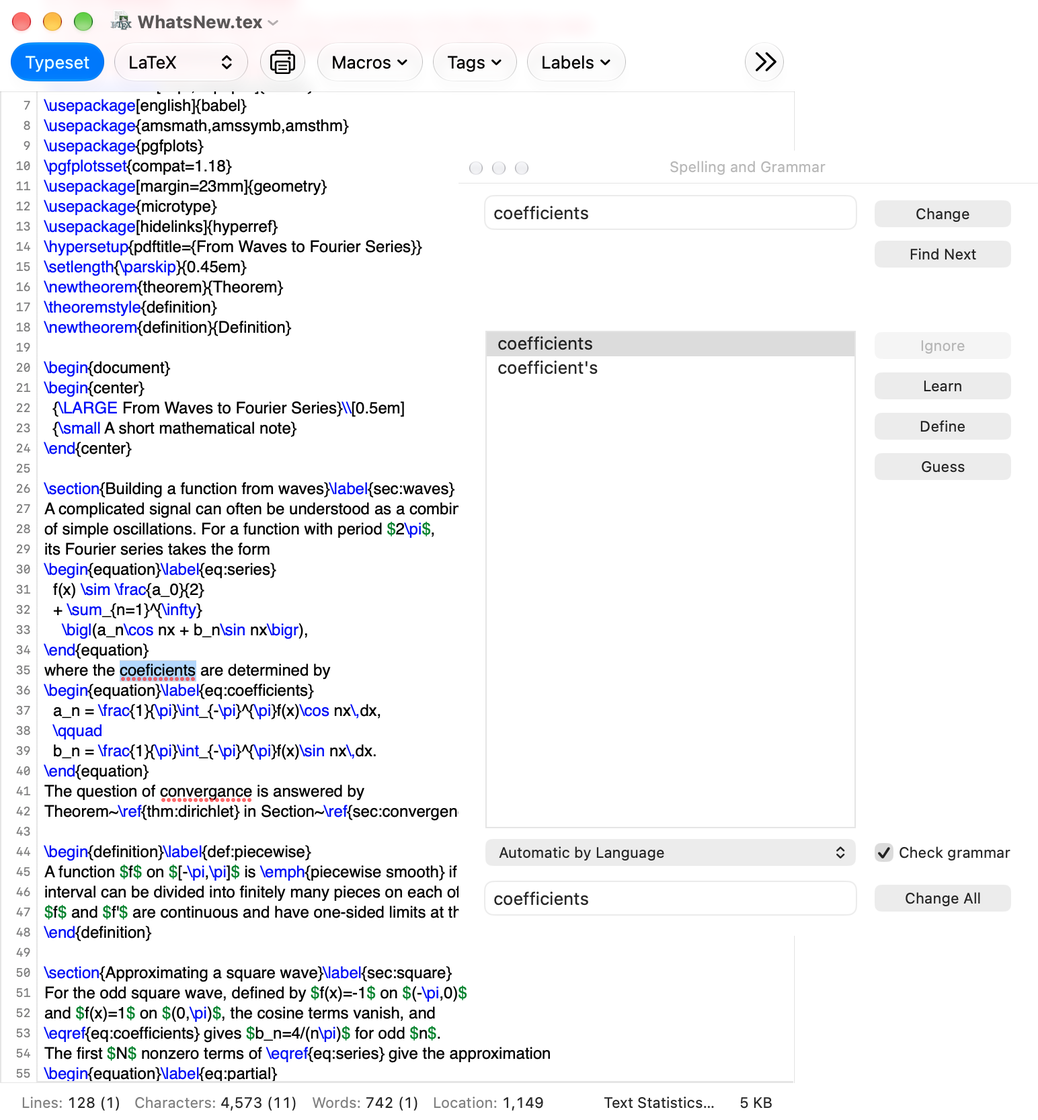
\includegraphics[width=0.8\textwidth]{Graphics/manual-spell.png}
   \caption{The Spelling and Grammar panel checking a source with LaTeX-aware spell checking}
   \label{fig:SpellingPanel}
\end{figure}

\section{Checking a Document}\label{SpellCheckingDocument}

The commands are in the submenu \mnu{Edit}\To\mnu{Spelling and Grammar}.

\begin{description}
\item[\mnu{Check Spelling While Typing}] underlines misspelled words as you type. Whether a document starts with this on is set by \mnu{Check spelling while typing} in the \mnu{Spell Checking} category of TeXShop Settings; it is on by default.
\item[\mnu{Show Spelling and Grammar} (\cmdkey-:)] opens the Spelling and Grammar panel, which shows the first misspelled word after the insertion point. The word is selected and the window scrolls so that its line is in the middle. Click \mnu{Find Next} in the panel to go on to the next one.
\item[\mnu{Check Document Now} (\cmdkey-;)] goes to the next misspelled word without the panel.
\item[\mnu{Check Grammar With Spelling}] also marks grammar mistakes, as in other applications of macOS.
\item[\mnu{Correct Spelling Automatically}] changes words as you type into what macOS thinks you meant. It is off by default, which suits \TeX, where it would also change commands. The item \mnu{Correct Spelling} in the \mnu{Spell Checking} category of TeXShop Settings sets whether it is on in the windows that open.
\item[\mnu{Forget Learned Words\ldots}] lists the words of the active document that were learned for the current language; the words you select are removed from the dictionary.
\item[\mnu{Edit Spelling Exclusions\ldots}] opens the rules of LaTeX-aware spell checking (\cref{SpellingExclusionRules}).
\end{description}

Hold down the Option key while choosing \mnu{Show Spelling and Grammar} or \mnu{Check Document Now}, or while clicking \mnu{Find Next}, to use the search of macOS, which skips no markup.

The panel has an additional field, \mnu{Replacement for Change All}, with a button \mnu{Change All}. Type a replacement there, or select a suggestion in the panel's list, by clicking it or with the arrow keys, which copies the suggestion into the field; when there is only one suggestion, it is filled in as soon as the word is shown. Click \mnu{Change All}, or press Return in the field, to replace every occurrence of the word in the text being checked; one Undo takes back the whole change. \mnu{Change} and \mnu{Change All} act on the word just found; after you have selected other text or edited the document, click \mnu{Find Next} first.

\mnu{Help}\To\mnu{TeXShop Help} describes spell checking too, in the language of TeXShop when it has its own help.

\section{LaTeX-aware Spell Checking}\label{LaTeXAwareSpellChecking}

The \mnu{Method} group of the \mnu{Spell Checking} category of TeXShop Settings has two choices: \mnu{Use LaTeX-aware spell checking (recommended)}, the default, and \mnu{Legacy method} (\cref{SpellCheckingLegacy}).

LaTeX-aware spell checking skips comments, mathematics, \TeX\ commands, and the arguments of commands such as \verb|\label|, \verb|\ref|, \verb|\cite| and \verb|\usepackage|, and checks the rest of the text. The rules that come with TeXShop also skip the arguments that are not prose, such as keys, colors and units, of the commands of common packages, among them hyperref, cleveref, xcolor, siunitx, enumitem, biblatex and natbib.

The macros that the document defines with \verb|\newcommand|, \verb|\def| and similar commands are read, so an argument that a definition only passes on to \verb|\ref|, into mathematics and the like is skipped too; and a command that the document defines itself, such as a macro of your own named \verb|\unit|, follows its own definition rather than the rule for the package command of that name.

Text marked as another language with \verb|\foreignlanguage|, \verb|\selectlanguage|, the \verb|otherlanguage| environment and the like is checked in that language by the panel and by \mnu{Check Document Now}, but is not underlined while typing.

LaTeX-aware spell checking works with the Spelling and Grammar panel, \mnu{Check Document Now} and \mnu{Check Spelling While Typing}, which then does not underline the skipped parts of the source. It applies to \TeX\ source files and to new documents not yet saved. Other files, such as Sweave files, are always checked with the legacy method.

\subsection{Exclusion Rules}\label{SpellingExclusionRules}

What is skipped is described by rules in the file
\begin{verbatim}
~/Library/TeXShop/SpellCheck/SpellingExclusions.txt
\end{verbatim}
Open it with the button \mnu{Edit LaTeX exclusion rules\ldots} at the end of the line of LaTeX-aware spell checking in TeXShop Settings, or with \mnu{Edit}\To\mnu{Spelling and Grammar}\To\mnu{Edit Spelling Exclusions\ldots}; it opens in TeXShop. The top of the file explains its format. For example, these lines skip the first argument of a command \verb|\mycommand| and the contents of the \verb|proof| environment:
\begin{verbatim}
skip-args  1  mycommand
skip-body  proof
\end{verbatim}
Changes take effect the next time spelling is checked. If the file is deleted, TeXShop makes a new copy of the default file the next time it starts.

\section{Dictionaries}\label{SpellCheckingDictionaries}

\mnu{Dictionary} in the \mnu{Check Spelling} group of the \mnu{Spell Checking} category of TeXShop Settings chooses the dictionary of documents opened from then on; documents already open keep theirs. The menu shows each language under its own name, such as Deutsch or Fran\c{c}ais, with its code, such as \texttt{de} or \texttt{fr\_CA}, as the tool tip. \mnu{Automatic Language} lets macOS choose the language from the text.

To use another dictionary for one document, choose it in the pop-up menu at the bottom of the Spelling and Grammar panel while that document is in front. Each open document keeps its own dictionary, and the panel switches when you switch documents. The choice is not kept when the document is closed.

To give a document its dictionary every time it opens, put a line like this among its first 20 lines:
\begin{verbatim}
% !TEX spellcheck = de-DE
\end{verbatim}
The value is a language code, as in the tool tips of the \mnu{Dictionary} menu: \texttt{fr} for French, or \texttt{fr\_CA}, also written \texttt{fr-CA}, for the French of Canada. The line is read when the document is opened, so save, close and open the document again after adding it. In a document with chapter files, put the line in each file.

The hidden setting \texttt{OriginalSpelling} leaves the language entirely to the Spelling and Grammar panel, as in other applications, instead of keeping a dictionary for each document; see \cref{chap:hidden-settings}.

\section{The Legacy Method}\label{SpellCheckingLegacy}

With \mnu{Legacy method} chosen in the \mnu{Method} group, macOS checks everything in the source except what the three options below it leave out. They are off by default.

\begin{description}
\item[\mnu{Do not check LaTeX commands}] skips command words such as \verb|\documentclass|, \verb|\usepackage| and \verb|\alpha|.
\item[\mnu{Do not check selected parameters}] skips the first two parameters, in brackets or braces, of a built-in list of commands whose parameters hold special words, such as \verb|\usepackage[parfill]{parskip}|, while the parameters of other commands, such as \verb|\emph{...}|, are checked. The hidden setting \texttt{ExtraCommandsNotToCheckParameters} adds commands to this list (\cref{chap:hidden-settings}).
\item[\mnu{Do not check comments}] skips comments.
\end{description}

These options work only while syntax highlighting is on, and \mnu{Check Document Now} does not follow them. The options remain visible, and keep their values, while LaTeX-aware spell checking is chosen.

% ===== 17-panels-tools.tex
\chapter{Panels and Tools}\label{PanelsToolsChapter}

\section{The LaTeX Panel}\label{LaTeXPanelSection}

\mnu{Window}\To\mnu{LaTeX Panel...} (\optkey-\cmdkey-hyphen) opens a panel of \LaTeX\ code: mathematical symbols, Greek letters, functions, accented and international characters, environments and typeface commands (\cref{fig:latexpanel}). Click in the source where the code should go, then click a button in the panel; its code is inserted at the insertion point. The panel is shown while a source window is in front, and steps aside while a Preview window is in front.

\begin{figure}[htbp]
   \centering
   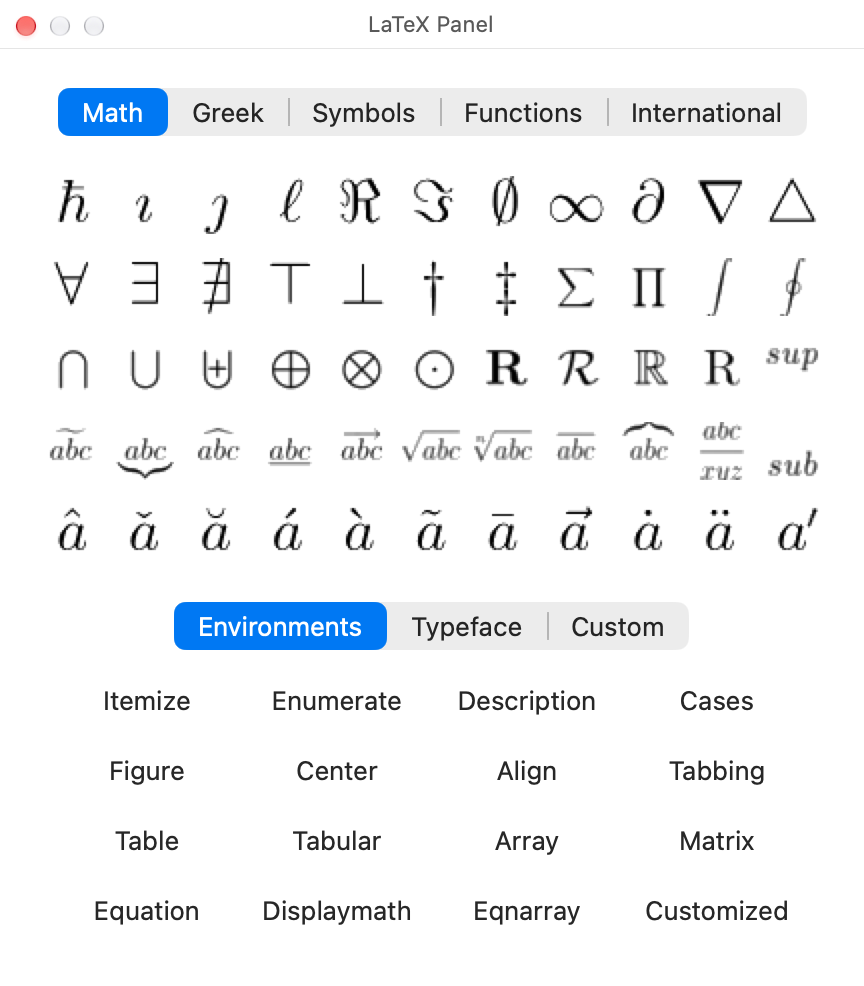
\includegraphics[width=3in]{Graphics/latexpanel.png}
   \caption{The LaTeX Panel, showing the Math and Environments pages}
   \label{fig:latexpanel}
\end{figure}

The panel has two halves, each with a segmented control at its top that chooses a page of buttons: \mnu{Math}, \mnu{Greek}, \mnu{Symbols}, \mnu{Functions} and \mnu{International} in the upper half, and \mnu{Environments}, \mnu{Typeface} and \mnu{Custom} in the lower half. The buttons of the upper half show the symbols they insert; those of the lower half show their names. If text is selected when you click a typeface or environment button, the selected text goes inside the inserted code, as in \verb|\textbf{selected text}|. Some symbols need the \texttt{amssymb} package; add \verb|\usepackage{amssymb}| to the preamble of a document that uses them.

The code that each button inserts, and the buttons of the \mnu{Custom} page, can be changed; see \cref{LaTeXPanelCustomizing}.

\section{The Matrix Panel}\label{MatrixPanelSection}

\mnu{Window}\To\mnu{Matrix Panel...} (\optkey-\cmdkey-=) opens a panel that writes matrices and tables (\cref{fig:matrixpanel}). Type the entries into its table as in a spreadsheet, choose how the result should look, and insert it into the source at the insertion point. Like the LaTeX Panel, it is shown while a source window is in front.

\begin{figure}[htbp]
   \centering
   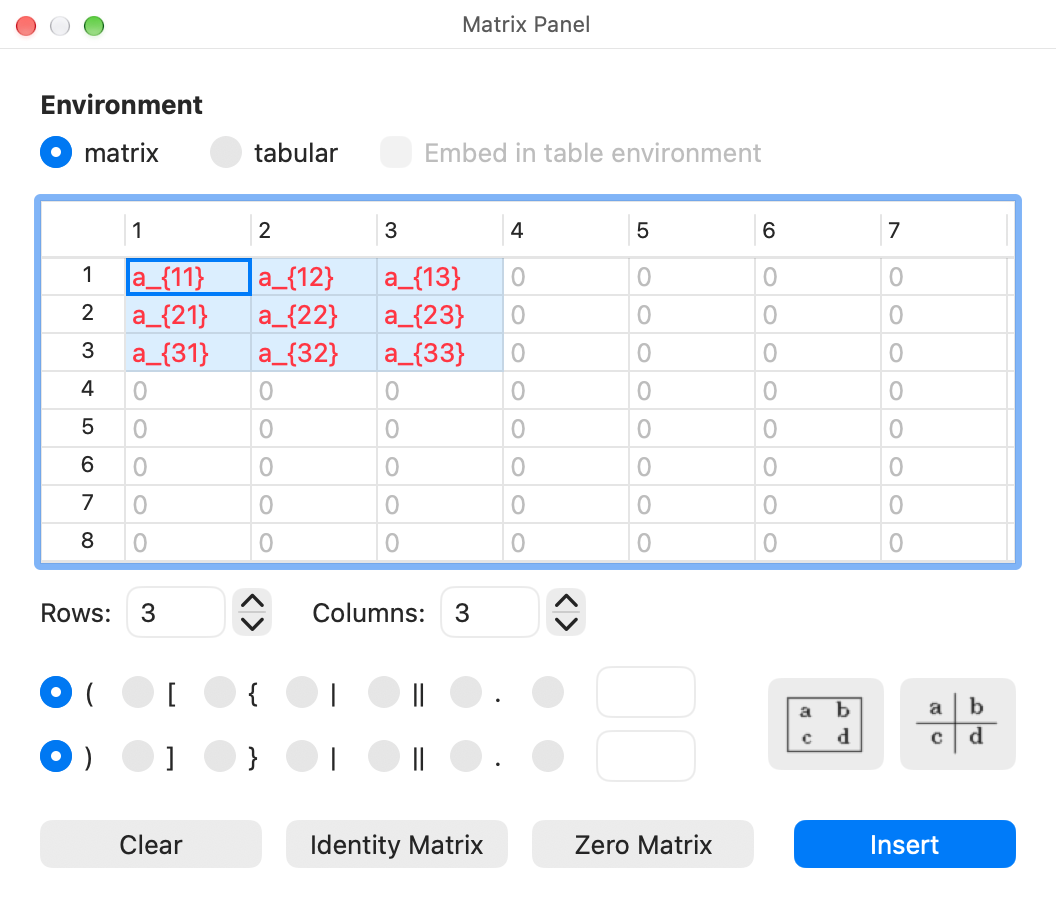
\includegraphics[width=0.75\textwidth]{Graphics/matrixpanel.png}
   \caption{The Matrix Panel with a $3\times3$ matrix}
   \label{fig:matrixpanel}
\end{figure}

\subsection{Writing a Matrix}

\begin{enumerate}
\item Enter the size in \mnu{Rows:} and \mnu{Columns:}, or change it with the arrows beside them, up to 999 each. The cells that will be inserted are shown on blue; the tool tip of the table says so: ``Only the blue cells are inserted''.
\item Type the entries into the blue cells. For example, with 3 rows and 3 columns, type \verb|a_{11}|, press Tab, type \verb|a_{12}|, and so on; Return at the end of a row goes to the first column of the next one.
\item Under \mnu{Environment}, choose \mnu{matrix} for a matrix in a formula (an \texttt{array} environment) or \mnu{tabular} for a table of text. With \mnu{tabular}, \mnu{Embed in table environment} puts the table into a \texttt{table} float with a caption and a label.
\item For a matrix, choose the left and right delimiters: \verb|(|, \verb|[|, \verb|{|, \verb+|+ or \verb+||+. The period leaves that side without a delimiter, and the last choice uses the delimiter typed in the field beside it.
\item To add lines, click the two buttons with pictures of a matrix: \mnu{Draw border} puts a border around the entries and \mnu{Draw grid} puts lines between them. A button stays pressed while it is on.
\item Click \mnu{Insert}, or press \cmdkey-Return. \mnu{Insert} is the default button, so Return alone inserts too while the table is not active. An entry still being typed goes in as well.
\end{enumerate}

The matrix of the example, with parentheses, is inserted as follows, on one line:
\begin{verbatim}
\left(\begin{array}{ccc}a_{11} & a_{12} & a_{13} \\
a_{21} & a_{22} & a_{23} \\
a_{31} & a_{32} & a_{33}\end{array}\right)
\end{verbatim}

\mnu{Clear} empties all cells, and \mnu{Identity Matrix} and \mnu{Zero Matrix} fill them with an identity matrix or with zeros.

\subsection{Working in the Table}

\begin{description}
\item[Choosing cells] Click a cell to choose it. Drag, or Shift-click, to choose a range of cells. Click the number of a row at the left, or the number of a column at the top, to choose the whole row or column; Shift-click another number to add the rows or columns up to it. Click the corner above the row numbers, or press \cmdkey-A, to choose every cell.
\item[Typing] Type to replace the value of the chosen cell. To change a value instead, double-click the cell, or press F2 or Control-U. While editing, Escape puts back the value the cell had.
\item[Moving] Return moves down and Tab moves right; with Shift, they move up and left. After a row of entries typed with Tab, Return goes to the next row in the column where you started. The arrow keys move one cell, and with Shift they extend the range chosen. \cmdkey-arrow goes to the last row or column that is inserted, and then to the end of the table; \cmdkey-Up Arrow and \cmdkey-Left Arrow go to the first row and column. Home and End go to the first and to the last inserted column of the row, and \cmdkey-Home and \cmdkey-End to the first cell and to the last inserted cell. Page Up and Page Down move by a screenful. Moving past the last row or column adds a row or a column to the table.
\item[Deleting, copying and pasting] Delete empties the cells chosen. Cut, Copy and Paste of the \mnu{Edit} menu work on the cells chosen, and exchange cells with spreadsheet applications such as Numbers and Excel, as text with tabs between the cells. A single value pasted fills every cell chosen; several values are pasted from the first cell chosen.
\item[Moving rows and columns] Drag the number of a row up or down to move the row, and drag the number at the top of a column sideways to change the order of the columns. The matrix is inserted in the order shown.
\item[Undo] \mnu{Edit}\To\mnu{Undo} and \mnu{Redo} take back and redo the changes of the table while the panel is active, including \mnu{Clear}, \mnu{Identity Matrix} and \mnu{Zero Matrix}.
\end{description}

When the matrix is made smaller, the cells outside it keep their values, shown in gray, and they come back when it is made larger again. Make the panel larger to see more of the table; it can be as large as the screen. The panel remembers the widths and the order of its columns.

\subsection{Changing the Code}

The code the panel writes around the entries is kept in \path{~/Library/TeXShop/MatrixPanel/matrixpanel_1.plist}: the beginning and end of the environments, the delimiters, the separators between entries and between rows, the lines of a border or grid, and the letter \texttt{c} that sets the alignment of each column. For example, change \texttt{c} to \texttt{r} to align the columns to the right. Keep the number and the order of the strings in the file, and restart TeXShop after changing it.

\section{Character Info}\label{CharacterInfoSection}

The source window can hold text in any script, so it is sometimes useful to know exactly which Unicode characters a piece of text contains. Select the text and choose \mnu{Edit}\To\mnu{Character Info...}, which is also in the contextual menu of the source. A popover at the selection describes it.

\begin{figure}[htbp]
   \centering
   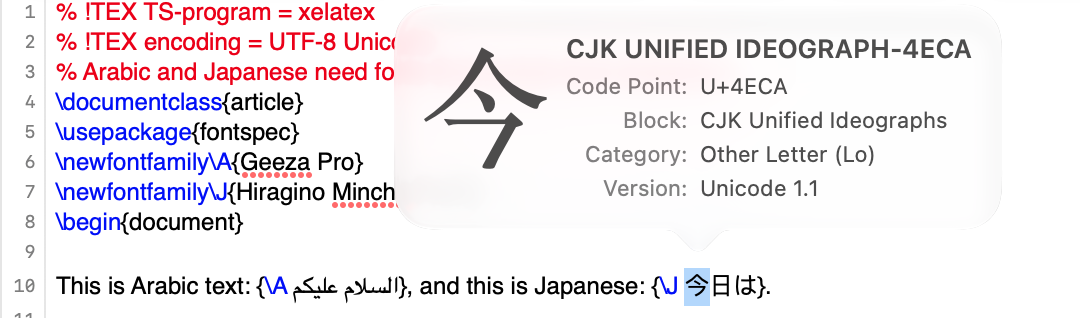
\includegraphics[width=0.85\textwidth]{Graphics/charinfo-single.png}
   \caption{Character Info for a single character}
   \label{fig:charinfoSingle}
\end{figure}

\paragraph{A single character.} When one character is selected, the popover shows the character enlarged, its Unicode name, and a table of its \mnu{Code Point}, the Unicode \mnu{Block} it belongs to, its general \mnu{Category} and the \mnu{Version} of Unicode that added it (\cref{fig:charinfoSingle}). A code point that UTF-16 writes as a surrogate pair is followed by the two halves of the pair, and a character that Unicode deprecates is marked \mnu{deprecated}. Spaces and control characters are shown as their control pictures. Click a translated block name to see the name Unicode gives it, and click again to see the translation.

A single character can consist of several code points, such as a letter with a combining accent, or an emoji sequence. The popover then says so in place of the name, as in ``<a character consisting of 2 code points>'', shows no table, and lists each code point with its name. Click the triangle in front of a code point to see its glyph, its block and its category. When the second code point is a variation selector or an emoji skin tone modifier, the name says which variant or tone is selected, the table describes the first code point, and the two code points are listed below it.

\begin{figure}[htbp]
   \centering
   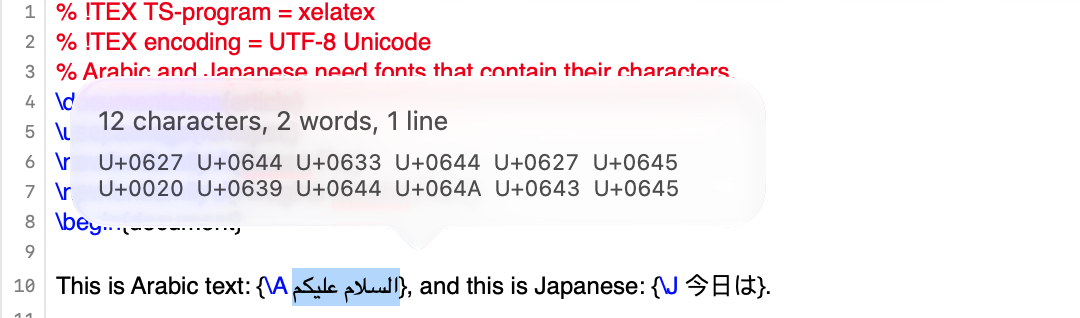
\includegraphics[width=0.85\textwidth]{Graphics/charinfo-several.png}
   \caption{Character Info for a piece of Arabic text}
   \label{fig:arabic}
\end{figure}

\paragraph{Several characters.} When several characters are selected, the popover shows the number of characters, words and lines, counted as in the status bar under the source, such as ``12 characters, 2 words, 1 line'', and the code points of the selection, which can be selected and copied. \Cref{fig:arabic} shows it for a piece of Arabic text.

\section{Experiments}\label{ExperimentsSection}

\mnu{Edit}\To\mnu{Experiment...} lets you try a short but tricky piece of \LaTeX, such as a formula, a table or a TikZ picture, before you put it into the document. It is available when a source window is active.

\begin{figure}[htbp]
   \centering
   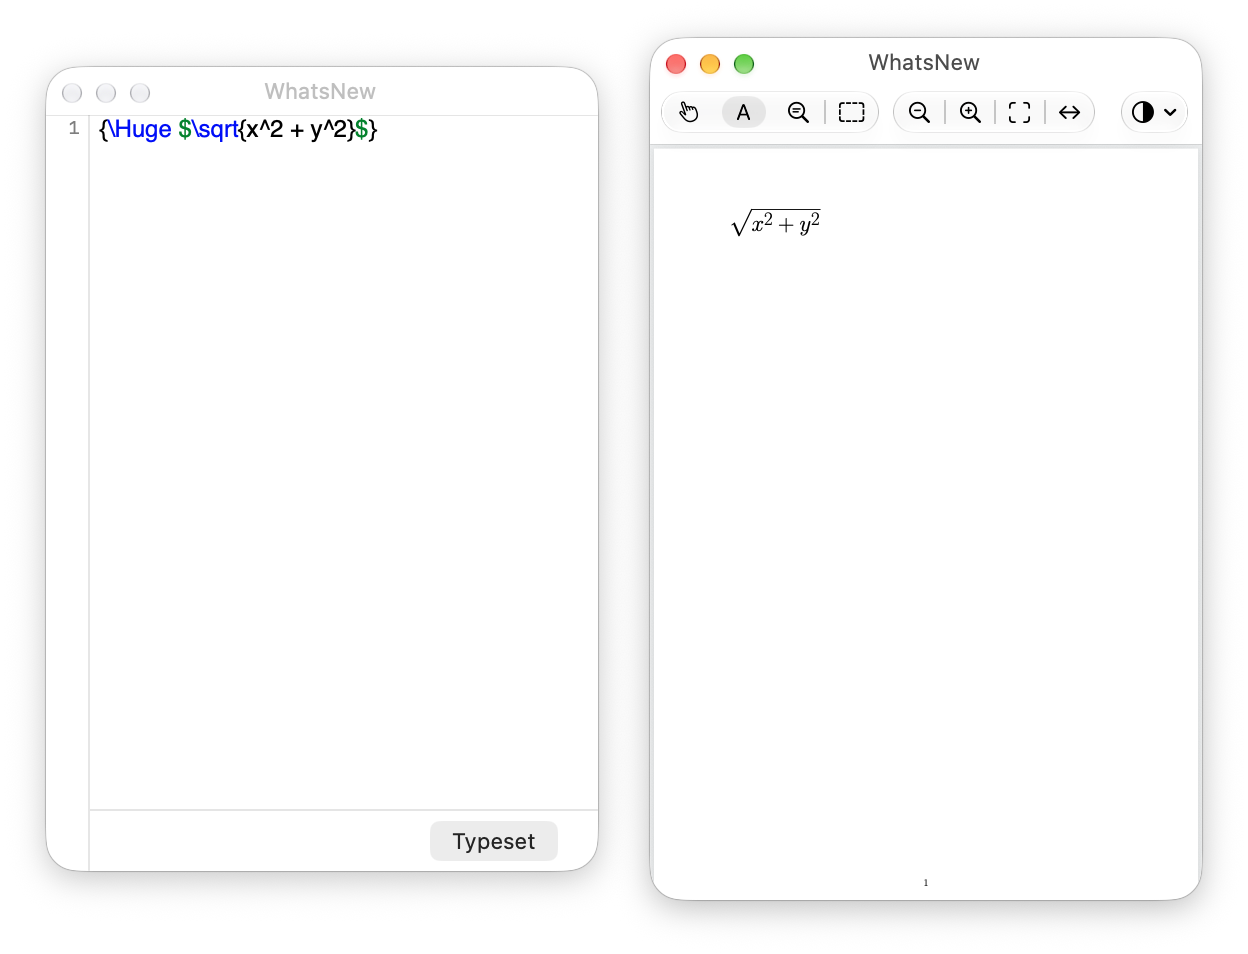
\includegraphics[width=\textwidth]{Graphics/experiment.png}
   \caption{The source panel and the preview panel of an experiment}
   \label{fig:experiment}
\end{figure}

The command opens a source panel. If text is selected in the source window, it is copied into the panel; otherwise the panel shows what you left in it last time, so a fragment can be brought back for another change. Type or edit the fragment, for instance
\begin{verbatim}
$$\sqrt{x^2 + y^2}$$
\end{verbatim}
and click the \mnu{Typeset} button at the bottom of the panel. A preview panel shows the result (\cref{fig:experiment}). When you change the fragment and typeset again, the preview keeps the part of the page you are looking at. The fragment can be anything from a formula to several pages.

\subsection{How the Fragment Is Typeset}

TeXShop typesets a file made of the preamble of the document, everything up to \verb|\begin{document}|, followed by the fragment and \verb|\end{document}|. In a project with a root file, the preamble of the root file is used. The document and its folder are not changed:
\begin{itemize}
\item The file is typeset in a temporary folder that holds copies of the files and folders next to the document, so pictures are found as when the document is typeset, usually also with paths that begin with \verb|./|, such as \verb|\graphicspath{{./figures/}}|.
\item A copy of the \texttt{.aux} file of the last typesetting of the document is read, so \verb|\ref|, \verb|\pageref| and \verb|\cite| show the numbers of the document.
\end{itemize}

The engine is the one the document uses: a \verb|% !TEX program| line at the top of the source, or else the choice in the toolbar of the source window. With LaTeX, the typesetting method of the document is followed: Direct PDF, Via DVI or Personal Script, as set in the \mnu{Typesetting} category of TeXShop Settings. If BibTeX or MakeIndex is chosen, pdfLaTeX is used. ConTeXt, MetaPost and plain \TeX\ cannot be used for an experiment. Engines of your own are tried, but they may fail if they do not expect \LaTeX\ or do not produce a PDF file.

\subsection{The Panels}

The source panel shows text as the source window does, with the same font, tabs, line spacing, wrapping, syntax colors, current line highlight, block cursor, invisible characters, line numbers and bracket matching. \cmdkey-+ and \cmdkey-- enlarge or reduce the text. Key bindings, command completion and label and citation key completion work in the panel; command completion uses the trigger key chosen with \mnu{Completion trigger} in the \mnu{Keyboard} category of TeXShop Settings. The Advanced Find panel finds text in the source panel and in the Experiment console too (\cref{AdvancedFind}).

The toolbar of the preview panel has the mouse tools of the Preview window: Scroll, Select Text, Magnify and Select PDF (\cref{Preview_Mouse_Tools_Section}). With Select PDF, draw a rectangle and copy it in the format chosen in \mnu{Preview}\To\mnu{Copy Format}. Beside the tools are Zoom Out, Zoom In, Zoom to Content, which enlarges the typeset part of the page to fill the panel, and Zoom to Content Width, which makes the typeset part as wide as the panel and shows its top at the top of the panel. The panel also scrolls and zooms with the mouse and with trackpad gestures.

The output of typesetting appears in a console of its own, the Experiment console. It comes to the front when typesetting starts; click a panel to bring that panel forward again. \cmdkey-0 (\mnu{File}\To\mnu{Show Console}) in a panel brings the Experiment console forward, and pressing it again returns to the panel. If the \mnu{Console} category of TeXShop Settings is set to show the console only when an error occurs, the Experiment console stays hidden until \TeX\ reports an error or waits for input.

The panels and the Experiment console float above the document windows. They are named after the document, and can be moved and resized; TeXShop remembers their sizes and places. Close a panel with its close button or \cmdkey-W.

\subsection{Keeping the Result}

When the fragment is right, copy it from the source panel and paste it into the document. The panels keep their contents when they are closed and reopened, but not when TeXShop quits, and they cannot be saved. Each document has its own panels; with several documents open, close the panels you no longer need, so that it stays clear which document an experiment belongs to. Commands of the menus, such as \mnu{Source}\To\mnu{Comment}, act on the source window, not on the source panel.

\section{Writing Tools}\label{WritingToolsSection}

On a Mac with Apple Intelligence, the Writing Tools of macOS work in the source window. Select one or more paragraphs, and choose \mnu{Writing Tools} from the contextual menu of the source (Control-click) or from the \mnu{Edit} menu. Writing Tools can proofread the text or rewrite it, for example to make it more concise, more professional or more friendly, and it lets you accept the result or go back to the original text. The Writing Tools interface is part of macOS, not of TeXShop.

Writing Tools leaves most \LaTeX\ commands alone, but not always all of them; after rewriting a passage, check that the document still typesets, for instance that every \verb|\begin{...}| still has its \verb|\end{...}|. It is best used on passages of prose rather than on whole documents.

% ===== 18-themes.tex
\chapter{Themes and Syntax Highlighting}\label{ThemesChapter}

\section{Themes}\label{ThemesSection}

The colors of TeXShop's windows, of syntax highlighting, of matching brackets, of invisible characters and of other highlights form a \emph{theme}. Themes are chosen and edited in the \mnu{Themes} category of TeXShop Settings (\cref{fig:Theme}).

\begin{figure}[htbp]
   \centering
   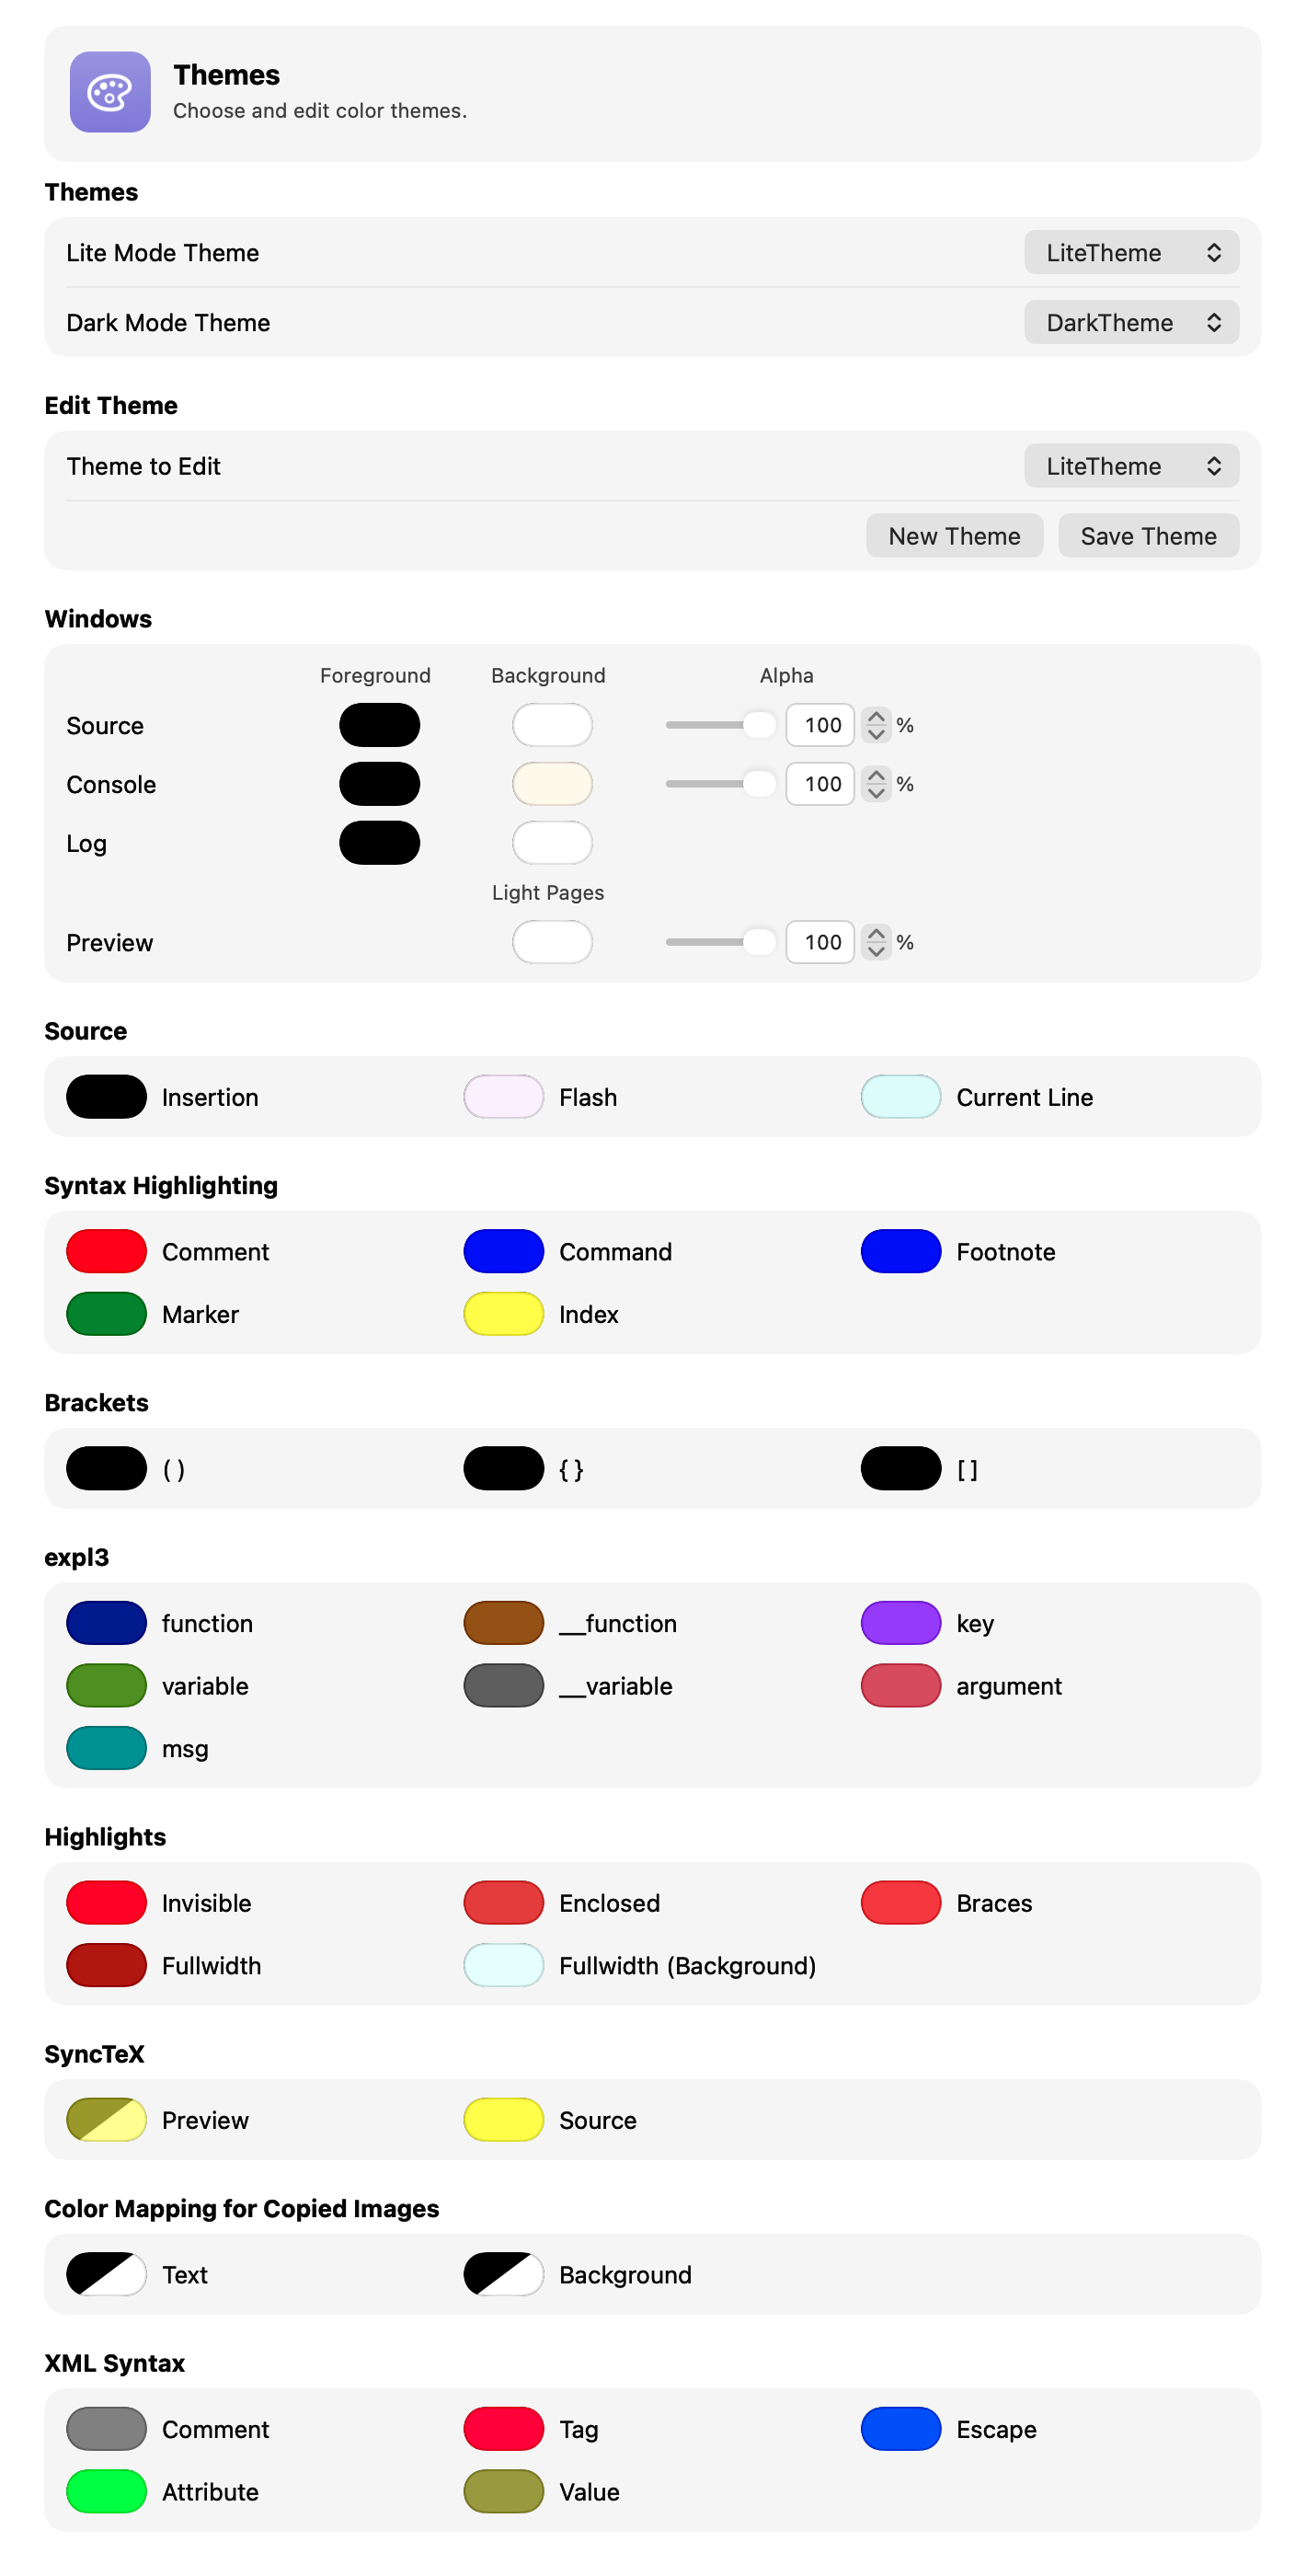
\includegraphics[height=0.85\textheight,keepaspectratio]{Graphics/SettingsThemes.png}
   \caption{The Themes category of TeXShop Settings}
   \label{fig:Theme}
\end{figure}

The pop-up menus \mnu{Light Mode Theme} and \mnu{Dark Mode Theme} choose the theme used while macOS is in Light Mode and in Dark Mode; any theme can be used in either mode, and both can be set to the same theme. TeXShop comes with several themes: LiteTheme and DarkTheme, the default themes of the two modes, and others such as SolarizedLite, SolarizedDark, Dracula and TransparentTheme. \Cref{fig:DarkThemeLightPages} shows a source window in DarkTheme next to a preview with light pages.

\begin{figure}[htbp]
   \centering
   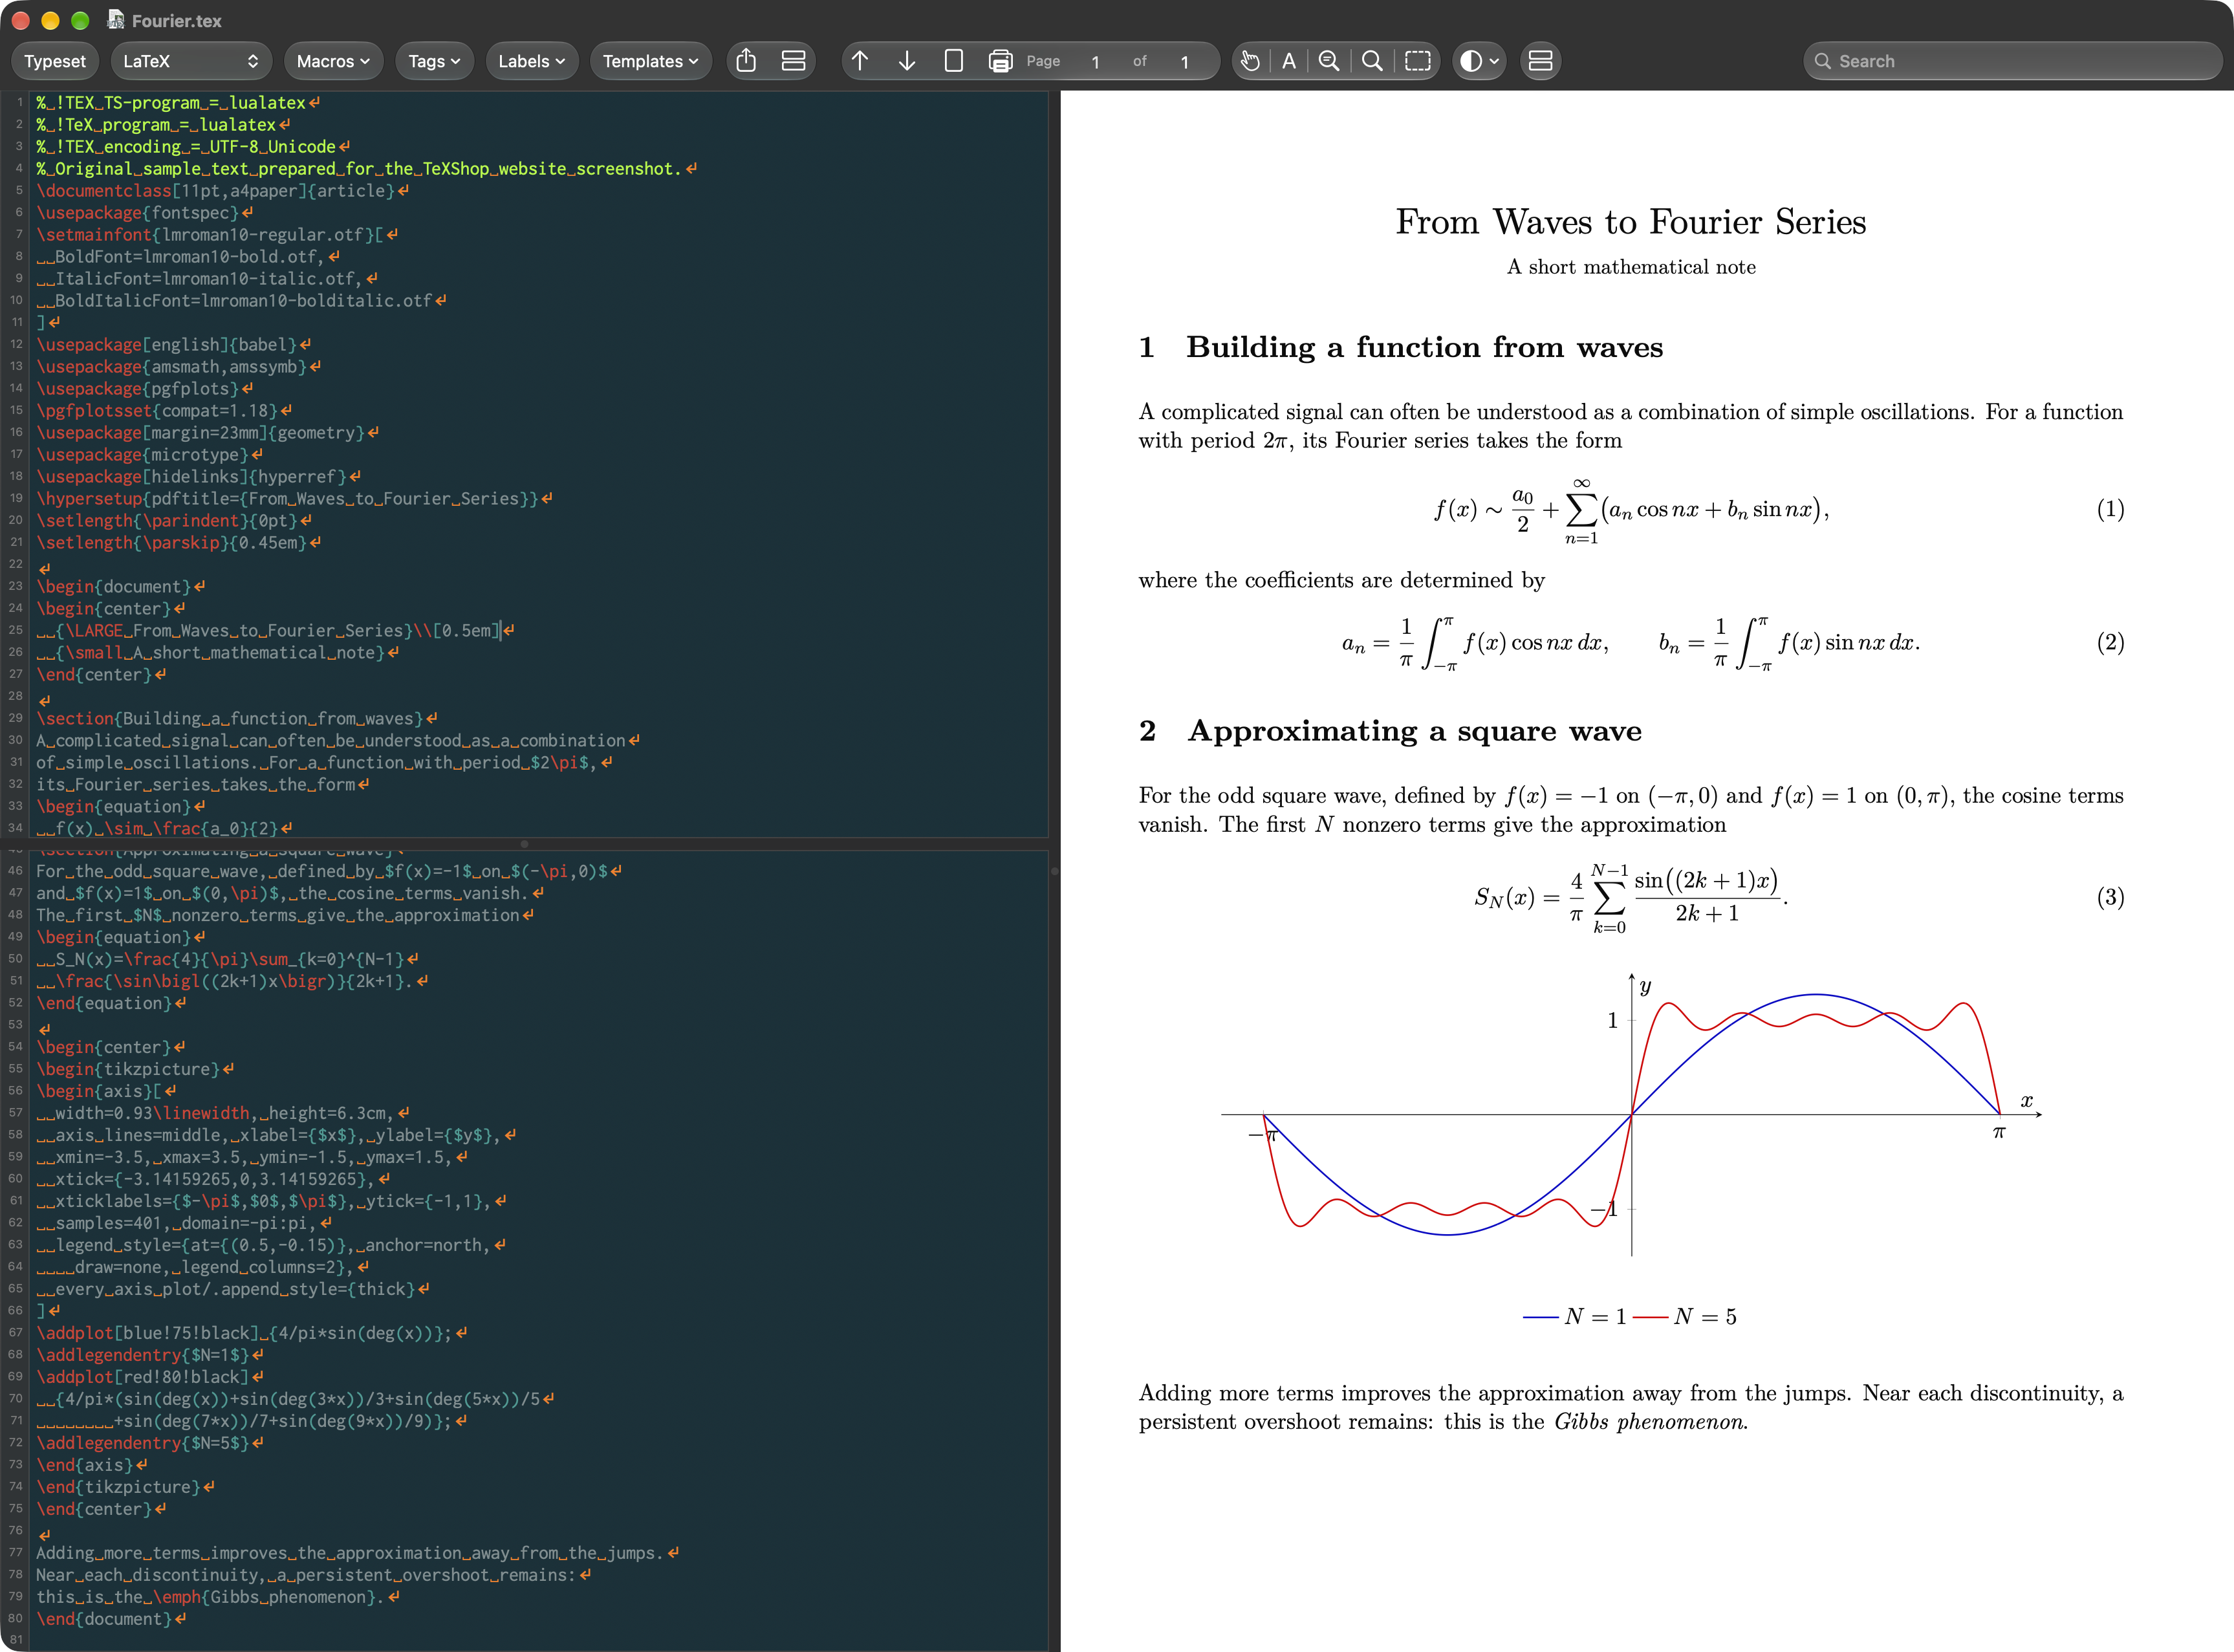
\includegraphics[width=\textwidth]{Graphics/manual-theme-dark_page-light.png}
   \caption{A window with DarkTheme; the pages of the preview are shown light}
   \label{fig:DarkThemeLightPages}
\end{figure}

\subsection{Managing Themes}\label{ManagingThemesSection}

Under \mnu{Edit Theme}, all themes are listed; the colors shown below the list are those of the theme selected in it. A sun marks the theme used in Light Mode and a moon the theme used in Dark Mode. Below the list are a plus button, a minus button and an actions menu (the button with three dots at the right end); Control-click a theme in the list for a contextual menu.
\begin{itemize}
\item \textbf{Add.} The plus button adds a theme with TeXShop's colors for the current appearance (those of LiteTheme in Light Mode, of DarkTheme in Dark Mode). Type its name, and begin changing its colors.
\item \textbf{Duplicate.} \mnu{Duplicate} makes a copy of the theme, to change while keeping the original.
\item \textbf{Rename.} \mnu{Rename} edits the name in the list. A theme used in Light Mode or Dark Mode stays in use under its new name.
\item \textbf{Delete.} The minus button, or \mnu{Delete} in the contextual menu, moves the theme to the Trash after asking. A theme used in Light Mode or Dark Mode gives way to LiteTheme or DarkTheme.
\item \textbf{Restore.} \mnu{Restore} gives a theme that comes with TeXShop its original colors again. A dot marks such a theme whose colors were changed.
\item \textbf{Export.} \mnu{Export\ldots} saves a copy of the theme's file, for example to use it on another Mac or to give it to others. A theme can also be dragged from the list to the Finder. With the Option key held down, \mnu{Show in Finder} takes the place of \mnu{Export\ldots} and shows the theme's file in the Finder.
\item \textbf{Import.} \mnu{Import\ldots}, in the actions menu, adds theme files saved by \mnu{Export\ldots}. Theme files can also be dropped on the list. An imported theme whose name is taken gets a number after its name.
\end{itemize}
In the actions menu, the items name the selected theme, as in \mnu{Duplicate ``SolarizedLite''}; the contextual menu acts on the theme clicked. The themes that come with TeXShop can be duplicated, restored and exported, but not renamed or deleted. If LiteTheme or DarkTheme is missing, TeXShop puts it back.

Changes to a theme are saved at once, and open documents follow them. If the theme file cannot be saved, the colors return to the last saved ones and an error is shown.

The themes are kept as small \texttt{.plist} files in \path{~/Library/TeXShop/Themes}. Each lists its colors, with the red, green, blue and alpha values of each color as numbers between zero and one. Change the colors in Settings rather than in these files.

\section{The Colors of a Theme}\label{ThemeColorsSection}

The colors are grouped by their purpose.

\begin{description}
\item[Windows] The foreground and background colors of the source, the console and the log, and the background of the Preview window's pages while they are shown light (the column under \mnu{Light Pages}). For each of these except the log, the opacity of the window, under \mnu{Alpha}, is set with a slider and a numeric field, from 0\% (transparent) to 100\% (opaque); use the arrow buttons beside the field to raise or lower it by one percent. The colors themselves are always opaque, so their color wells offer no opacity.

\item[Source] The colors of the insertion point (\mnu{Insertion}), the \mnu{Flash}, the \mnu{Current Line} and the \mnu{Selection}. Under the insertion point and the selection is a \mnu{Use system color} switch. When it is on, the source uses the system's color instead: the accent color for the insertion point and the highlight color for the selection, as chosen in System Settings \To\ Appearance, and the color well shows that color. The theme keeps its own color, which comes back when the switch is turned off. In the themes that come with TeXShop, the insertion point uses the theme's color and the selection the system's. The same insertion point and selection colors are used in the source panel of Experiments, in the contents of the Macro Editor and in the fields of the Advanced Find panel. While a window is in the background, its selection is shown in the system's gray. \mnu{Current Line} is the background of the line with the insertion point while \mnu{Source}\To\mnu{Highlight Current Line} is on. \mnu{Flash} is the color the source window flashes when a closing bracket without a matching opening bracket is typed, if \mnu{Flash Back for Isolated Parens} is on in the \mnu{Matching Brackets} group of the \mnu{Editor} category.

\item[Syntax Highlighting] \mnu{Comment}, \mnu{Command}, \mnu{Footnote}, \mnu{Marker} and \mnu{Index}; see \cref{SyntaxHighlightingSection}.

\item[Brackets] The colors of \verb|( )|, \verb|{ }| and \verb|[ ]|.

\item[expl3] The seven colors of expl3 highlighting (\cref{expl3Chapter}). Each theme that comes with TeXShop sets them to suit its palette; a theme without them uses built-in expl3 colors.

\item[Highlights] \mnu{Invisible} is the color of invisible characters shown with \mnu{Source}\To\mnu{Show Invisible Characters}. \mnu{Enclosed} and \mnu{Braces} are used by the options of the \mnu{Matching Brackets} group of the \mnu{Editor} category. \mnu{Fullwidth} and \mnu{Fullwidth (Background)} are the text and background colors of fullwidth letters, digits and symbols, the characters U+FF01 to U+FF5D except the fullwidth comma and full stop, and of the minus sign U+2212; in Japanese text these characters are easily mistaken for their ASCII counterparts. \mnu{Highlight Fullwidth Letters and Symbols} in the \mnu{Syntax Highlighting} group of the \mnu{Editor} category turns this highlight off; the theme keeps the colors. A theme without the Fullwidth colors shows these characters like other text; its color wells then show the text and background colors of the source, and choosing a color adds it to the theme.

\item[SyncTeX] The colors that mark the place found by synchronization in the \mnu{Preview} and in the \mnu{Source}.

\item[Color Mapping for Copied Images] When \mnu{Use Color Mapping} is on in the \mnu{Copy Images} group of the \mnu{Preview} category, a selection copied, dragged or saved from the preview as an image, rather than as PDF or EPS, has black replaced by the \mnu{Text} color and white by the \mnu{Background} color.

\item[XML Syntax] The colors of \mnu{Comment}, \mnu{Tag}, \mnu{Escape}, \mnu{Attribute} and \mnu{Value} in HTML, XML and PreTeXt files.
\end{description}

The color of the block cursor is not part of the theme; it is set with \mnu{Cursor Color:} in the \mnu{Insertion} group of the \mnu{Editor} category.

\subsection{Light Pages}

PDF files made by \TeX\ have no background color, so that printing them puts black letters on white paper. The Preview window can therefore fill the pages with the background color of the theme; this color shows wherever the page is not covered by text or by a picture with its own background. It is not part of the PDF file and is not printed. The text color of the pages is set by the document itself; to change it, change the \LaTeX\ source.

The color fills the pages only while they are shown light. When the \mnu{Appearance} item in the toolbar of the Preview window shows the pages dark, they are not filled, so that they look deep black.

\section{Syntax Highlighting}\label{SyntaxHighlightingSection}

The source window shows \TeX\ in colors. \mnu{Source}\To\mnu{Syntax Highlighting} turns highlighting on or off for the active document; documents open with it on. Files that are not \TeX\ sources, such as log files, are not highlighted; the list of extensions that count as \TeX\ sources is in \cref{OpeningOtherFilesSection}.
\begin{itemize}
\item Comments have the Comment color.
\item Commands, a backslash followed by letters, have the Command color. \mnu{@ as Part of Command Names} in the \mnu{Syntax Highlighting} group of the \mnu{Editor} category of TeXShop Settings also counts \verb|@| as a letter, as in the internal commands of packages.
\item The argument of \verb|\footnote| and of citation commands such as \verb|\cite|, \verb|\footcite| and \verb|\autocite| has the Footnote color.
\item The markers \verb|$| and \verb|&| have the Marker color, and the brackets \verb|( )|, \verb|{ }| and \verb|[ ]| each have their own color.
\item \mnu{Source}\To\mnu{Highlight Index Entries} shows the arguments of \verb|\index| and \verb|\esindex| in the Index color. \mnu{Highlight Index Entries by Default} in the \mnu{Syntax Highlighting} group of the \mnu{Editor} category turns it on when documents open.
\end{itemize}
The hidden settings \texttt{SyntaxColoringEnabled} and \texttt{SyntaxColorFootnote} open documents with highlighting off and color only the footnote command; see \cref{chap:hidden-settings}. HTML, XML and PreTeXt files are highlighted with the XML Syntax colors.

\section{expl3 Syntax Highlighting}\label{expl3Chapter}

expl3 is the programming layer of modern \LaTeX: a set of programming conventions designed for large \TeX\ macro projects such as \LaTeX\ itself. Its documentation is the package \texttt{expl3} on CTAN (\url{https://ctan.org/pkg/expl3}); see also \url{https://www.latex-project.org/latex3/}.

\mnu{Source}\To\mnu{Highlight expl3 Code} turns expl3 highlighting on or off. When it is on, the ordinary highlighting still applies, and expl3 code is given its own colors in addition; there is coloring only while \mnu{Source}\To\mnu{Syntax Highlighting} is on. Like most items of the Source menu, it applies to the active document, so expl3 highlighting can be on in one source window and off in another. Since most users use \LaTeX\ macros rather than write them, documents open with it off; \mnu{Highlight expl3 Code by Default} in the \mnu{Syntax Highlighting} group of the \mnu{Editor} category of TeXShop Settings turns it on when documents open.

\subsection{What Is Colored}

With expl3 highlighting on, the underscore \verb|_|, the colon \verb|:| and \verb|@| count as letters of command names, in addition to \verb|a|--\verb|z| and \verb|A|--\verb|Z|. Any other character ends the name. A name gets one of the colors of the \mnu{expl3} group of the theme:

\begin{description}
\item[function] A name that contains both an underscore and a colon, such as
\begin{verbatim}
\tl_set:Nn   \clist_pop:NN   \mymodule_function:Nn
\end{verbatim}
A name without an underscore, or without a colon, is an ordinary command.
\item[variable] A name that begins with \verb|l_|, \verb|g_| or \verb|c_| (local, global and constant variables), such as
\begin{verbatim}
\l_mymodule_localvariable_clist   \g_mymodule_globalvariable_int
\c_mymodule_constant_str
\end{verbatim}
\item[\_\_function] A function whose name begins with two underscores, an internal function that other packages should not rely on, such as \verb|\__tl_set:Nn|.
\item[\_\_variable] A variable whose name has two underscores after its first letter, such as
\begin{verbatim}
\l__mymodule_localvariable_clist   \g__mymodule_globalvariable_int
\end{verbatim}
\item[msg] A name that begins with \verb|msg_|, such as \verb|\msg_error:nnn|.
\item[key, argument] A command that sets the value of a key: the name of the key, optional spaces, then on the same line a period that begins a string without spaces containing at least one underscore or colon. The name of the key gets the key color; the period and the rest of the string get the argument color. For example:
\begin{verbatim}
thiskey .tl_set:N = {...}
akey.is_nothing = {hello}
\end{verbatim}
\end{description}

% ===== 19-saving.tex
\chapter{Saving Documents}\label{SavingChapter}

\section{Autosave and Versions}\label{AutosaveSection}

TeXShop uses the autosave of macOS. While you edit, the source is saved automatically every few minutes, and
also whenever it has to be: before it is typeset, when its window is closed, and when TeXShop quits. Only the
changes are written, so saving goes unnoticed. You never need to save a document before typesetting it.

The title of a window whose text has changed since it was last saved shows ``Edited''. \mnu{File}\To\mnu{Save}
(\cmdkey-S) saves the document at once and removes this mark. Undo works across saves, so changes that turned out
badly can be undone even after they have been saved.

The file on disk contains only the current text of the document. Earlier versions are kept by macOS outside the
file, so a file you copy or send to someone else contains nothing of what you deleted before.

With autosave, the \mnu{File} menu has \mnu{Duplicate}, which makes a copy of the document in a new window; to
save the document under another name, choose \mnu{Save As...}, which macOS shows when the Option key is held down
in the \mnu{File} menu.

\subsection{Turning Autosave Off}

Autosave is turned on and off by \mnu{Enable Autosave and Versions} in the \mnu{Saving Documents} group of the
\mnu{Documents and Saving} category of TeXShop Settings. A change takes effect when TeXShop is started again. Leave it
on unless there is a particular reason: TeXShop is designed and tested with autosave. While autosave is off:
\begin{itemize}
\item A document is saved when you choose \mnu{File}\To\mnu{Save} and when it is typeset. When a window with unsaved
changes is closed, or TeXShop quits, you are asked whether to save the changes.
\item The \mnu{File} menu has \mnu{Save As...} (\shiftkey-\cmdkey-S) and \mnu{Revert To Saved}, which goes back to the
file as it was last saved; macOS keeps no earlier versions, so \mnu{Browse All Versions...} is not available.
\item The switch \mnu{Keep the previous file as ``name\textasciitilde'' when saving}, just below
\mnu{Enable Autosave and Versions}, can be turned on: each time a file is saved, the previous file is kept as a
backup, with a tilde before the extension: \texttt{paper.tex} is kept as \texttt{paper\textasciitilde.tex}.
\end{itemize}

\section{Revert To}\label{RevertToSection}

To go back to an earlier state of a document, choose \mnu{File}\To\mnu{Revert To}. Its submenu goes back to the
version that was last saved or opened, and \mnu{Browse All Versions...} shows the current document beside a stack of
its earlier versions, each with the date and time it was saved. These versions are live: you can scroll through
them, copy text from an earlier version into the current one, or restore an earlier version completely. This needs
no Time Machine backup; macOS keeps the versions of each document itself.

\section{Locking a Document}\label{LockSection}

A document you want to keep as it is, such as a paper finished long ago, can be locked. Click the name of the
document in the title bar of its window and select \mnu{Locked} in the panel that opens. A locked document cannot be
changed or saved. Clear \mnu{Locked} in the same panel to edit it again. The same panel can also rename the document
and move it to another folder. This panel is there while autosave is on.

\section{Finding the File on Disk}\label{FindingDiskVersionSection}

Click the title of a source or Preview window while holding down the Command key: a menu lists the folders that
contain the file, from its own folder up to the disk. Choose a folder to open it in the Finder.

To see where a document is at a glance, add the \mnu{FullPath} item to the toolbar of the source window with
\mnu{Window}\To\mnu{Customize Toolbar...}; its tool tip is ``Show Full Path in Window Title''. Click it to show the full
path of the file, instead of its name, in the title of the source window, and also in the titles of its Preview window,
its console and its Experiment panels (\cref{ExperimentsSection}). Click it again to show the name. Documents opened
later start with the last choice.

% ===== 20-preview.tex
\chapter{The Preview Window}\label{PreviewChapter}

The Preview window shows the typeset PDF file. It is updated after every typesetting and stays at the page you were
reading. Its settings are in the \mnu{Preview} category of Settings: the items under \mnu{When a Document Opens} set
how a window starts, and the \mnu{Preview} menu changes them for the window in front while it is open.

Command-click in the Preview to go to the matching place in the source (SyncTeX, \cref{sec:synctex}).
\mnu{Window}\To\mnu{Source ⇔ Preview} (\cmdkey-1) switches between the source and its Preview. A Preview window you
have closed opens again at the same place, with \cmdkey-1 or after the next typesetting.
\mnu{Preview}\To\mnu{Save Preview Position} makes new Preview windows open at the place and size of the window in
front.

The contextual menu of the Preview opens when you click a page with the Control key held down, with the right mouse
button, or with two fingers on a trackpad. Its first items are \mnu{Sync}, which goes to the source like
Command-click, \mnu{Split Window}, \mnu{Split Window with Link} over a link (\cref{Split_Window_With_Link_Section}), and
\mnu{Link Popups} (\cref{Popup_Windows_Section}).

When another application, such as latexmk or an external editor, rewrites the PDF file, the Preview reloads it at the
same place. Turn on \mnu{Always Watch for PDF Changes by Other Apps} in the \mnu{Refresh} group of the \mnu{Preview}
category to have it reloaded also while TeXShop is in the background.

\section{The Toolbar}\label{PreviewToolbarSection}

The toolbar of the Preview window uses the icons of Apple's Preview. Hold the pointer over an item to see what it
does. By default the toolbar has these items:
\begin{description}
\item[\mnu{Previous Page}, \mnu{Next Page}] turn the pages.
\item[\mnu{Back/Forward}] two chevrons that go back and forward through the places you have visited
(\cref{Back_Forward_Arrows_Section}).
\item[\mnu{Drawer}] shows or hides the drawer with the outline of the document (\cref{Drawer_Section}).
\item[\mnu{Print}] prints the typeset document (\cref{PrintingSection}).
\item[\mnu{Magnification}] the magnification in percent, with arrows that change it by steps. Click the word
\mnu{Scale} in front of it to open the Magnification menu (\cref{MagnificationSection}).
\item[\mnu{Go to page}] the number of the page shown and the number of pages. Type a page number and press Return to go
there.
\item[\mnu{Mouse Mode}] what the pointer does on the page (\cref{Preview_Mouse_Tools_Section}).
\item[\mnu{Appearance}] light or dark pages (\cref{PreviewAppearanceSection}).
\item[\mnu{Page Layout}] the display format (\cref{DisplayFormatsSection}).
\item[\mnu{Two-Page Arrangement}] the order of pages shown side by side (\cref{TwoPageArrangementSection}).
\item[\mnu{Share Preview}] offers the PDF file to the sharing services of macOS, such as Mail and AirDrop.
\item[\mnu{Split Preview}] splits the window into two parts (\cref{Splitting_Windows_Section}).
\item[\mnu{Search PDF}] searches the text of the document (\cref{Drawer_Section}).
\end{description}
Choose \mnu{Window}\To\mnu{Customize Toolbar...} to add, remove and arrange items. Other items that can be added
include \mnu{Typeset}, \mnu{Program} and \mnu{Macros}, buttons for single programs such as \mnu{LaTeX} and
\mnu{BibTeX}, and \mnu{Zoom to Content} with its two buttons, Zoom to Content and Zoom to Content Width. Control-click
the toolbar to show icons only or icons with their names. Items that do not fit in a narrow window move into a menu
that opens from the button marked $\gg$ at the right end of the toolbar.

A window that shows the source and the Preview together (\cref{OneWindowSection}) has one toolbar with items of both.

\section{Display Formats}\label{DisplayFormatsSection}

\mnu{Preview}\To\mnu{Display Format} chooses how the pages are laid out:
\begin{description}
\item[\mnu{MultiPage}] all pages one below the other, in one long column that scrolls continuously. This is the
format most people use.
\item[\mnu{Double MultiPage}] pairs of pages side by side, in one long column.
\item[\mnu{Single Page}] one page.
\item[\mnu{Double Page}] one pair of pages side by side.
\end{description}
The \mnu{Page Layout} item of the toolbar opens a menu with the same four formats, each with an icon that shows how the
pages are laid out (\cref{fig:PageLayoutMenu}). \mnu{Default Page Style} under \mnu{When a Document Opens} sets the
format a window starts with.

\begin{figure}[htbp]
   \centering
   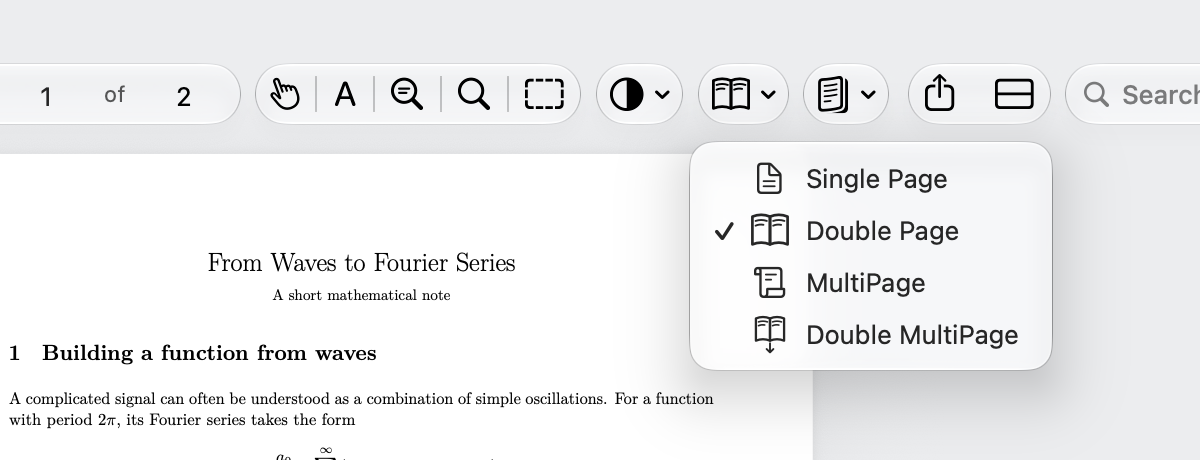
\includegraphics[width=0.8\textwidth]{Graphics/manual-toolbar-page-layout.png}
   \caption{The Page Layout menu of the toolbar}
   \label{fig:PageLayoutMenu}
\end{figure}

\mnu{Previous Page} and \mnu{Next Page}, in the \mnu{Preview} menu and in the toolbar, turn the pages, and the
\mnu{Go to page} field of the toolbar goes to a page by its number. The Up and Down Arrow keys scroll within the page.
The Left and Right Arrow keys scroll sideways when a magnified page is wider than the window, and otherwise turn the
page; turn on \mnu{Always turn pages with the left and right arrow keys} in the \mnu{Display and Navigation} group of
the \mnu{Preview} category to have them always turn the page.

In Single Page and Double Page, scrolling with the mouse wheel or the trackpad past the top or bottom of a page turns
the page, as in Apple's Preview. Turn on \mnu{Do not turn pages by scrolling} in \mnu{Display and Navigation} to have
scrolling stop at the edge of the page; the keyboard, the menu and the toolbar still turn the pages. Page Up and Page
Down turn the page when the whole page is shown, and otherwise scroll by a screen.

\subsection{Two Pages Side by Side}\label{TwoPageArrangementSection}

Two settings under \mnu{When a Document Opens} control the formats that show two pages side by side.
\mnu{Page direction} is \mnu{Left to Right}, or \mnu{Right to Left} for languages written from right to left, such as
Arabic, Hebrew and Persian, and for Japanese written vertically. \mnu{Show first page alone as cover}, on by default,
shows the first page by itself, followed by pairs of pages, as in a book: a book usually starts with an odd number of
preliminary pages, so the pairs on the screen are the pairs of facing pages of the printed book.

Magic comment lines set these properties for one document and take precedence over the settings:
\begin{verbatim}
     % !TEX bookDisplay
     % !TEX standardDisplay
     % !TEX PageDirectionL2R
     % !TEX PageDirectionR2L
\end{verbatim}
The first two show the first page alone or not; the last two set the page direction. When a document has no line for
the page direction, the reading direction recorded in the PDF file is used, if the file records one.

The \mnu{Two-Page Arrangement} item of the toolbar changes the arrangement of the document in the window while it is
open (\cref{fig:TwoPageArrangementMenu}): \mnu{Left to right} or \mnu{Right to left}, and
\mnu{Show first page alone as cover}. The icons of the menu show the pages in that order. \mnu{Restore Document
Settings} in the same menu returns to the settings and magic comment lines of the document.

\begin{figure}[htbp]
   \centering
   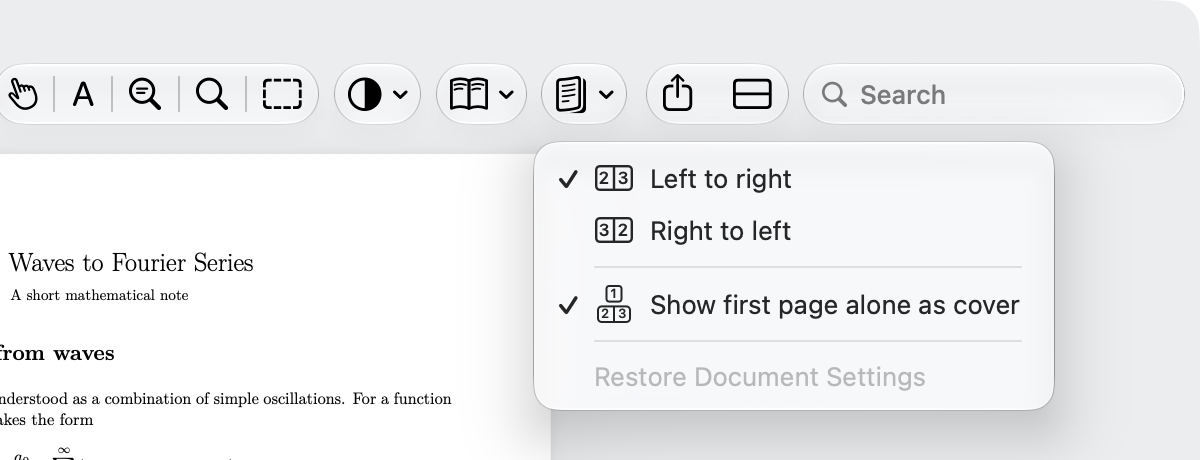
\includegraphics[width=0.8\textwidth]{Graphics/manual-toolbar-arrangement.png}
   \caption{The Two-Page Arrangement menu of the toolbar}
   \label{fig:TwoPageArrangementMenu}
\end{figure}

\section{Magnification}\label{MagnificationSection}

\mnu{Preview}\To\mnu{Magnification} offers four ways to set the magnification:
\begin{description}
\item[\mnu{Fit to Window}] The page fills the width of the window, and resizing the window changes the
magnification. This is the most convenient choice: on a large display, make the window show exactly one page; on a
smaller one, make it wide enough to read easily and scroll down through each page.
\item[\mnu{Fit to Content Width}] Like Fit to Window, but the white margins around the typeset part of the pages are
left out, so the text itself fills the width of the window. The magnification and the place sideways stay the same
as you scroll and turn the pages.
\item[\mnu{Fixed Magnification}] The magnification stays as set, whatever the size of the window.
\item[\mnu{Actual Size}] The pages appear at the size of the paper.
\end{description}
\mnu{After resizing the window} and \mnu{Magnification} under \mnu{When a Document Opens} set the choice and the
percentage a window starts with; the percentage is used with Fixed Magnification.

The \mnu{Magnification} field of the toolbar sets the percentage of the window, and the arrows beside it change it by
steps. Clicking the word \mnu{Scale} in front of the field opens the Magnification menu. \mnu{Zoom In}
(\shiftkey-\cmdkey-=) and \mnu{Zoom Out} (\shiftkey-\cmdkey--) in the Magnification submenu change the percentage by
steps, and spreading or pinching two fingers on a trackpad changes it freely. Each of these switches the window to
Fixed Magnification, so that resizing the window no longer changes the magnification. To go back, choose Fit to Window
or Fit to Content Width again.

Two commands at the end of the Magnification submenu change the magnification once:
\begin{description}
\item[\mnu{Zoom to Content}] The typeset part of the page in the middle of the window, without its white margins,
fits in the window.
\item[\mnu{Zoom to Content Width}] The typeset part fills the width of the window, and its top comes to the top of the
window.
\end{description}
Like the Magnification field, they switch the window to Fixed Magnification. The \mnu{Zoom to Content} item of the
toolbar has a button for each of them; add it with \mnu{Window}\To\mnu{Customize Toolbar...}. Keyboard shortcuts can be
given to them in the \mnu{Keyboard} category of Settings (\cref{KeyboardChapter}).

\section{Full Screen}\label{PreviewFullScreenSection}

\mnu{Window}\To\mnu{Enter Full Screen}, or the green button at the top left of the window, shows the Preview on the
whole screen. The window is unsplit and uses the magnification and display format last used in full screen; the first
time, these are Fit to Window and Double Page. Change them in full screen as you like, and TeXShop uses them the next
time. Leaving full screen brings back the earlier ones. To keep the split, the magnification and the display format of
the window instead, turn on \mnu{Keep magnification, display format and split when entering full screen} in
\mnu{Display and Navigation}.

\section{Light and Dark Pages}\label{PreviewAppearanceSection}

The \mnu{Appearance} item of the toolbar chooses how pages are drawn: \mnu{Light}, \mnu{Dark}, which shows the pages
with light text on a dark background, or \mnu{System}, which follows the appearance of macOS. The Preview color of the
theme in use (\cref{ThemesChapter}) gives the paper color of pages shown light.

\section{Mouse Tools}\label{Preview_Mouse_Tools_Section}

The \mnu{Mouse Mode} item of the toolbar chooses what the pointer does on the page:
\begin{description}
\item[\mnu{Scroll}] Drag to move the page.
\item[\mnu{Select Text}] Drag to select text, which can then be copied.
\item[\mnu{Magnify}] Press and hold to look through a small magnifying glass.
\item[\mnu{Magnify (Large)}] Press and hold to look through a larger magnifying glass.
\item[\mnu{Select PDF}] Drag to select an area of the page, to copy it as a picture.
\end{description}
\mnu{Default Mouse Mode} under \mnu{When a Document Opens} chooses the tool a window starts with.

\subsection{The Magnifying Glass}

With a Magnify tool, press and hold the mouse button to magnify the region near the pointer, and move the pointer to
magnify other regions. Double-click and hold for a larger glass, and triple-click and hold to magnify the whole
window. The glass works at any magnification of the Preview window and shows the page at 150\% of its size on the
screen. Hold down Command, Option or Control to raise this to 200\%, 250\% or 300\%; with Shift added, these keys give
100\%, 67\% and 50\% instead.

\subsection{Copying Parts of a Page}\label{CopyImagesSection}

With the Select PDF tool, drag over any part of a page; it can contain text, formulas and pictures. Copy it with
\cmdkey-C and paste it into another application, or drag the selection into a document of that application, such as a
Keynote slide. Dragging it to the desktop or a Finder window makes a file. \mnu{Preview}\To\mnu{Save Selection to
File...} saves the selection under a name and in a folder you choose. With the Select PDF tool,
\mnu{Edit}\To\mnu{Select All} selects everything shown: the page or pair of pages in Single Page and Double Page, and
the whole document in MultiPage and Double MultiPage, for documents of at most 20 pages.

The kind of picture made is set by \mnu{Image Copy Type} in the \mnu{Copy Images} group of the \mnu{Preview} category:
PDF, which keeps text and lines sharp at any size and is the default, or TIFF, JPEG or PNG, some in several qualities.
\mnu{Preview}\To\mnu{Copy Format} shows and changes the same setting.

For TIFF, JPEG and PNG pictures, two more items of the Copy Images group apply. \mnu{Use Color Mapping} turns black into
a text color and white into a background color, both set in \mnu{Color Mapping for Copied Images} of the current
theme, so that a copy matches the colors of a slide. \mnu{Foreground Prominence:} sets how strongly the text is
emphasized. PDF copies keep the colors of the page.

\section{Back, Forward and Rotation}\label{Back_Forward_Arrows_Section}

The \mnu{Back/Forward} item of the toolbar has two chevrons, as in a web browser and in Apple's Preview. They move
through the places you have visited in the document, for instance by following links or by typing page numbers in the
\mnu{Go to page} field. If you follow a link from a reference to a theorem, the left chevron takes you back to the
reference, and the right chevron then takes you to the theorem again. \mnu{Preview}\To\mnu{Back} and \mnu{Forward} do
the same. In a window that shows the source and the Preview together, add the item with
\mnu{Window}\To\mnu{Customize Toolbar...}.

\mnu{Preview}\To\mnu{Rotate Clockwise} and \mnu{Rotate Counterclockwise} turn all pages of the document by a quarter
turn.

\section{The Drawer and the Search Fields}\label{Drawer_Section}

\mnu{Preview}\To\mnu{Drawer}, or the \mnu{Drawer} item of the toolbar, shows or hides the drawer at the side of the
window.

The upper part of the drawer is the outline of the document: its chapters, sections and subsections. Click an entry to
go there. The entries can also be chosen with the keyboard: the Up and Down Arrow keys move from entry to entry,
Option-Up Arrow and Option-Down Arrow choose the first and the last entry, the Right Arrow key opens an entry with a
triangle and the Left Arrow key closes it, and Return or Enter goes to the chosen entry. Entries you open stay open
when the document is typeset again. The outline is empty when the PDF file has none.

The hyperref package writes the outline. A typical command to load it is
\begin{verbatim}
  \usepackage[colorlinks=true, pdfstartview=FitV, linkcolor=blue,
    citecolor=blue, urlcolor=blue, hyperfigures=true,
    bookmarksnumbered]{hyperref}
\end{verbatim}
The option \texttt{bookmarksnumbered} numbers the chapters and sections in the outline. Then an entry can be chosen by
typing its number while the drawer is active: type 2 and 0 for Chapter 20, or, with the sections of Chapter 1 shown,
1.5 for Section 5 of Chapter 1. Press Return to go there.

The lower part of the drawer is a search field. Type a word and press Return: every occurrence is listed below the
field with its page and the text around it. Click one to go there.

The \mnu{Search PDF} field of the toolbar searches too: type a word and press Return to select its first occurrence,
and press \cmdkey-G for the next one. While the Preview window is in front, \cmdkey-F goes to this field.

\section{Links}\label{LinksSection}

Links made by the hyperref package work in the Preview: click a reference to a theorem, an equation or an entry of
the bibliography to go there, and the left chevron of Back/Forward returns. A web address opens in your web browser.

\section{Link Popups}\label{Popup_Windows_Section}

Hold the pointer over a link to see the linked place in a small window, a popup. For instance, holding it over a
reference to a theorem shows the theorem (\cref{fig:LinkPopup}). The popup goes away after about four seconds.

\begin{figure}[htbp]
   \centering
   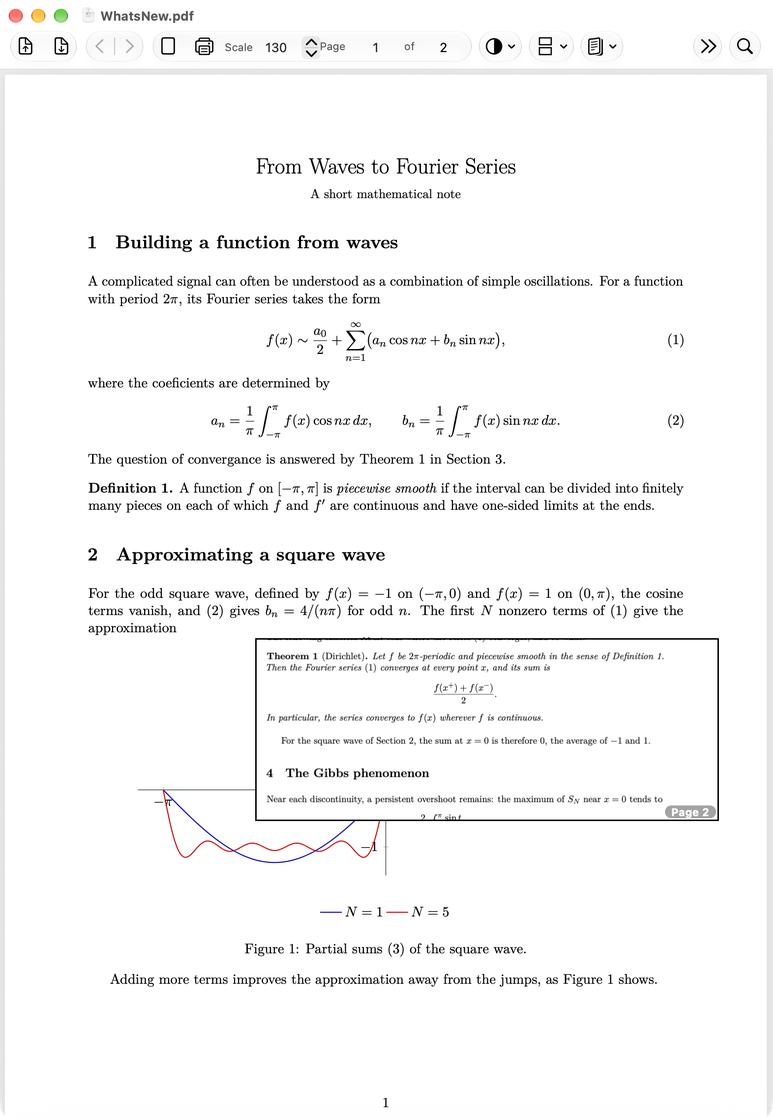
\includegraphics[width=0.55\textwidth]{Graphics/manual-link-preview.png}
   \caption{A link popup showing the theorem that a reference names, with its page number at the lower right}
   \label{fig:LinkPopup}
\end{figure}

The popup shows complete lines of the text column of the linked place. In MultiPage and Double MultiPage it goes on
with the top of the next page, so a theorem broken by a page break can be read in one popup.

The lower right corner of the popup shows the label of the linked page, such as ``Page 157''. This is the page number
given in the PDF, which may differ from the position of the page in the file, as in a book whose front matter is
numbered i, ii, \ldots. Turn off \mnu{Show page number in link popups} in \mnu{Display and Navigation} to leave it out.

\mnu{Preview}\To\mnu{Link Popups} turns the popups on and off for the window; the item is checked while they are on.
The same item is in the contextual menu of the Preview. The \mnu{Link Popups} switch under
\mnu{When a Document Opens} sets whether they are on when a document opens; it is on by default. No popups appear
while the Select PDF tool is chosen.

\subsection{Changing a Popup with Modifier Keys}\label{Modifying_Popup_Windows_Section}

Keys held down when the pointer reaches a link change its popup:
\begin{description}
\item[Shift] shows the popup above the link instead of below it.
\item[Command] shows a larger popup with larger text.
\item[Option] pins the popup, so that it stays (see below). Pressing Option while an ordinary popup is shown pins it
too.
\item[Control] reverses \mnu{Link Popups} for this link. While Link Popups is on, no popup appears, so that none gets
in the way of a Control-click that opens the contextual menu over the link. While Link Popups is off, the popup of the
link appears all the same.
\end{description}
The keys can be combined: Option-Shift, for instance, pins a popup shown above the link.

\subsection{Pinned Popups}\label{PinnedPopupsSection}

A pinned popup stays on the screen until you dismiss it, for instance while you move the pointer to explain how the
linked text relates to the page. You can go on working in the Preview: click, select text, scroll, zoom, turn pages and
follow links, and the popup stays at its place on its page.

A pinned popup can be moved by dragging it, and resized by dragging its edges or corners; resizing shows more or less
of the page at the same text size. Scrolling with the pointer over it scrolls the page inside it, which helps when the
interesting part, such as the end of a long formula, is not at the top. With the Scroll tool, dragging inside the
popup moves it; with the other tools, dragging over text selects it so that it can be copied, and dragging where
there is no text moves the popup.

To dismiss a pinned popup, press Escape in the Preview window. If you cannot see it, click in the Preview first to make
the window active. In full screen, the first Escape dismisses the pinned popup and a second one leaves full screen.
Turning off Link Popups also dismisses it.

While a popup is pinned, other links still show their popups. Pressing Option while one of them is shown pins it
instead of the popup pinned before: a window, or each part of a split window (\cref{Splitting_Windows_Section}), has
at most one pinned popup.

% ===== 21-windows.tex
\chapter{Organizing Windows}\label{WindowsChapter}\label{chap:windows}

A document in TeXShop has a source window, a Preview window and a console; a project with a root file and chapter
files has a source window for each file, and several projects can be open at once. TeXShop offers three ways to keep
these windows in order, which can be combined:
\begin{itemize}
\item separate source and Preview windows, as described so far;
\item one window that shows the source and the Preview of a document side by side;
\item tabs, which gather many windows into one.
\end{itemize}
In every arrangement, \mnu{Window}\To\mnu{Source ⇔ Preview} (\cmdkey-1) switches between the source and its Preview,
and \mnu{File}\To\mnu{Show Console} (\cmdkey-0) brings the console forward (\cref{ConsoleSection}). Choose an
arrangement and keep to it; mixing them can make windows open in unexpected places.

\mnu{Window}\To\mnu{Next Source Window} (\cmdkey-F2) and \mnu{Window}\To\mnu{Previous Source Window}
(\shiftkey-\cmdkey-F2) bring the open source windows forward one after another.

\mnu{Source}\To\mnu{Save Source Position} and \mnu{Preview}\To\mnu{Save Preview Position} record the place and size of
the window in front and set the \mnu{Window Positions} group of the \mnu{General} category of Settings to open new
windows there. A second pair, \mnu{Save Source Position for Portable} and \mnu{Save Preview Position for Portable},
records another position, for example for a laptop that is sometimes used with a large display; TeXShop opens the
windows at the saved position that fits the screen in use.

\section{One Window for Source and Preview}\label{OneWindowSection}

With a source window or its Preview window in front, choose \mnu{Window}\To\mnu{Use One Window}. The two windows
become one window with the source on the left and the Preview on the right. \mnu{Window}\To\mnu{Use Separate Windows}
splits it into two windows again. Both commands act on the document in front.

\mnu{Use One Window} needs a source file that has been saved and typeset, so that its PDF file exists. It does nothing
for a file with a \verb|% !TEX root| line: the combined window holds one source file and the Preview of that file. For
a project whose chapters are separate files, use separate windows; the root file can be shown in one window, but the
chapter files then open in windows of their own.

To have every document open in one window, set \mnu{Source and Preview} in the \mnu{Windows} group of the
\mnu{General} category of Settings to \mnu{Use One Window}. A new document still starts as a source window alone,
since there is nothing to preview yet: write the source, typeset it, and choose \mnu{Use One Window}. Do the same with a
source file that comes without its PDF file.

\mnu{Source position in the combined window}, in the same group, puts the source on the left or on the right. The
divider between the source and the Preview can be dragged; every combined window opens with the divider where you
left it last. To choose where combined windows open, arrange one and choose \mnu{Source}\To\mnu{Save Source Position}.

A combined window works well in full screen: click its green button or choose \mnu{Window}\To\mnu{Enter Full Screen},
and the whole screen shows the source and the Preview. When you typeset, the console floats over the window; close it
when you are done with it.

\section{Tabs}\label{TabsSection}

TeXShop windows can be gathered as tabs of one window, as in other macOS applications. \mnu{Open New Windows as Tabs}
in the \mnu{Windows} group of the \mnu{General} category of Settings chooses when this happens: \mnu{Never},
\mnu{Always}, or \mnu{Automatically}, which follows the macOS setting for preferring tabs when opening documents.

With \mnu{Always} and separate windows, each document you open adds a tab to the source window and a tab to the
Preview window, so two windows hold all open documents, including the files of projects with a root file. Consoles
and log files are gathered in the same way, each in a window of its own kind. Typesetting brings forward the tab of
the Preview that belongs to the source, and sync between source and Preview selects the matching tab. Each tab of the
Preview has its own drawer.

With \mnu{Always} and \mnu{Source and Preview} set to \mnu{Use One Window}, each tab holds one whole document, with its
source and Preview. A window with tabs can be taken to full screen, so that several documents can be worked on in full
screen, switching between them with the tabs.

\mnu{Use One Window} and \mnu{Use Separate Windows} act only on the document of the active tab. To move several
documents from tabs of separate windows into one window with tabs, choose \mnu{Use One Window} for each of them; the
second and later documents become tabs of the first combined window.

The switch ``Open files reached by Sync as tabs in the root file's window'' in the
\mnu{Source and Preview Synchronization} group of the \mnu{Typesetting} category is for projects with a root file: when
sync from the Preview opens a chapter file that is not open yet, the file joins the window of the root file as a tab
instead of opening its own window. So tabs appear just for the chapters you work on. The switch is off by default.

\subsection{Opening a Project in Tabs}\label{ProjectTabsSection}

The root file of a project can ask TeXShop to open its chapter files as tabs of its window. The following magic
comment lines do this; see \cref{MagicCommentsChapter} for magic comment lines in general. A root file with one of them
opens in separate source and Preview windows, also when \mnu{Source and Preview} is set to \mnu{Use One Window}.

Put this line in the first 20 lines of the root file:
\begin{verbatim}
     % !TEX useTabs
\end{verbatim}
When the root file opens, the files named in its \verb|\include| commands open as tabs. Short names for the tabs can
follow on the same line, in parentheses and separated by commas; a blank between two commas keeps the name of that
file:
\begin{verbatim}
     % !TEX useTabs (Intro, Groups, , Fields)
\end{verbatim}
To give the files of \verb|\input| commands tabs as well, use the hidden setting
\begin{verbatim}
     defaults write TeXShop TabsAlsoForInputFiles YES
\end{verbatim}

To choose the files yourself, put \texttt{useTabsWithFiles} in the first 20 lines of the root file, and a
\texttt{tabbedFile} line for each tab in the first 50 lines, for up to 20 tabs. A name for the tab can follow in
parentheses:
\begin{verbatim}
     % !TEX useTabsWithFiles
     % !TEX tabbedFile{chapter1/Introduction.tex} (Introduction)
     % !TEX tabbedFile{Galois.log}
     % !TEX tabbedFile{~/Graphics/diagram.pdf}
\end{verbatim}
A path is relative to the folder of the root file, starts at your home folder with \verb|~|, or is a full path. Always
write the extension: these tabs can also show log files, PDF files and pictures. Each file opens as it would if you
opened it yourself, so a source file may bring its Preview along.

\section{Splitting Windows}\label{Splitting_Windows_Section}

A source window or a Preview window can be split into two parts that show different places of the same document: one
part shows the passage you are writing about, the other the passage you are writing.

\mnu{Window}\To\mnu{Split Window} (\ctlkey-2) splits the window in front into a top and a bottom part, and unsplits it
when it is split. Hold down the Option key to choose \mnu{Window}\To\mnu{Split Window Vertically} (\ctlkey-\optkey-2),
which splits it into a left and a right part. The \mnu{Split Source} and \mnu{Split Preview} items of the toolbars do
the same; Option-click them to split side by side. While the Option key is held down, the icon of the item shows the
split that a click then makes. In a split window the item unsplits the window. The contextual menu of the Preview has
\mnu{Split Window} too.

In a window that shows the source and the Preview together, \mnu{Window}\To\mnu{Split Window} splits the source.
Split the Preview there with the \mnu{Split Preview} item of the toolbar or with \mnu{Split Window} in the contextual
menu of the Preview.

\begin{figure}[htbp]
   \centering
   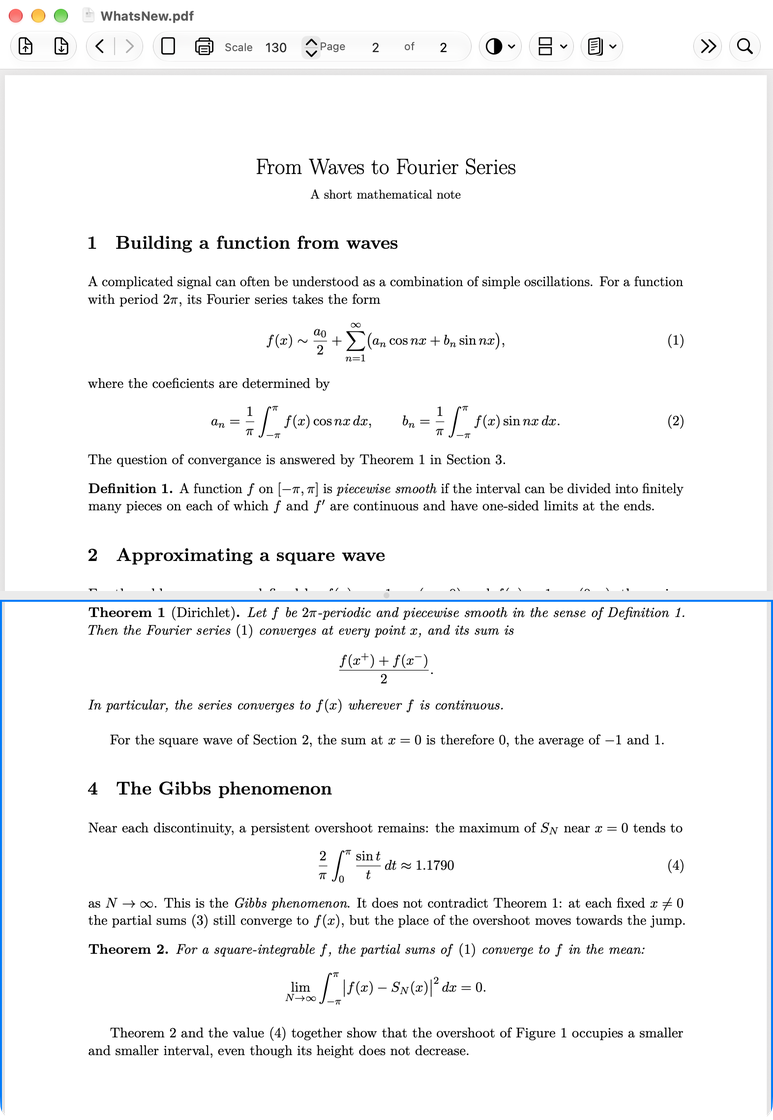
\includegraphics[width=0.55\textwidth]{Graphics/manual-split-preview.png}
   \caption{A split Preview window. \mnu{Split Window with Link} shows the theorem that a reference names in the
   bottom part, the active part.}
   \label{fig:SplitPreview}
\end{figure}

Each part of a split Preview window has its own place, display format, magnification and pinned link popup, and
typesetting updates both parts. Drag the divider to change the sizes of the parts. In MultiPage and Double MultiPage,
splitting the window into a top and a bottom part leaves the pages where they are on the screen: the divider comes over
the pages, and the bottom part shows what was below it. When the window is split again later, the parts come back with
the sizes and places they had.

\subsection{Two Ways to Split with Shift}\label{Options_Splitting_Horizontally_Section}

Hold down Shift while choosing \mnu{Split Window} or clicking the \mnu{Split Preview} item to split a Preview window
into a top and a bottom part of the same height. In MultiPage and Double MultiPage the bottom part shows what was below
the divider; in the other display formats both parts show the place that was at the top of the window. To split into
two parts of the same height without continuing the pages below the divider, hold down Shift and Control while
choosing \mnu{Window}\To\mnu{Split Window} with the mouse.

Shift-splitting suits a lecture given from a Preview window. When the lecture reaches a theorem, Shift-split the
window: the theorem stays in the top part, where students can refer back to its assumptions, while the bottom part
scrolls on through examples and the proof.

\subsection{The Active Part}\label{Active_View_Split_Window}

In a split window, one part is active: the part you clicked last. In a split source window it is the part with the
cursor. In a split Preview window the active part has a thin line in the accent color of macOS along its edges, while
the window is in front.

The commands of the window act on the active part:
\begin{itemize}
\item SyncTeX goes between the active part of the source and the active part of the Preview.
\item The menus, \mnu{Display Format} and \mnu{Magnification} among them, change the active part.
\item The \mnu{Go to page} field of the toolbar shows the page of the active part, and typing a page number there
moves the active part.
\item The drawer follows the active part: clicking an entry moves that part, and the drawer marks the chapter or
section shown in it.
\item Escape dismisses the pinned link popup of the active part (\cref{PinnedPopupsSection}).
\end{itemize}
Clicking in the drawer makes the drawer active; click in a part of the window to make that part active again.

\subsection{Showing a Link in the Other Part}\label{Split_Window_With_Link_Section}

Open the contextual menu of the Preview over an internal link, such as a reference to a theorem or an entry of the
table of contents, and choose \mnu{Split Window with Link}. The linked place appears in the other part of the window,
while the part with the link stays where it is (\cref{fig:SplitPreview}). If the window is not split, it is first
split into a top and a bottom part; hold down Option while choosing the item to split side by side. If the window is
already split, the other part moves to the linked place, whichever part contains the link.

The part that shows the linked place becomes the active part, so the left chevron of Back/Forward takes it back to
where it was. The item appears over links to places in the same document.

\section{Switch Views}\label{Switch_Views_Unsplit_Section}

\mnu{Window}\To\mnu{Switch Views} (\optkey-2) works in a separate Preview window.

In a split window, it exchanges the two parts. Each part takes along its place, display format, magnification and
pinned popup, and the sizes of the parts stay as they were.

In a window that is not split, Switch Views changes between two views of the document. Scroll to one passage you are
working on, choose Switch Views, and scroll to a second passage; from then on, \optkey-2 goes back and forth between the
two. Each view keeps its own place, display format, magnification and pinned popup, so one view can show a whole page
with Fit to Window while the other shows a detail at a high magnification. To revise a passage shown in either view,
sync from it to the source, edit, and typeset.

\subsection{Switch Views and Split Windows Together}\label{Independence_Split_Window_Section}

The two views of a window that is not split are separate from the bottom part of a split window, so you can work with
three views. Splitting the window makes the view shown the top part; the bottom part is a view of its own. After the
window is unsplit, \optkey-2 still shows the other view of Switch Views.

None of these changes touch the PDF file: splitting, switching views and changing the display only change how
TeXShop shows the file.

% ===== 22-printing-console.tex
\chapter{Printing and the Console}\label{PrintingConsoleChapter}

\section{Printing}\label{PrintingSection}

To print the typeset document, choose \mnu{File}\To\mnu{Print...} (\cmdkey-P) in the Preview window or in the source
window. In a project with a root file, the typeset root document is printed. The \mnu{Print} item of the Preview
toolbar prints the typeset document as well.

The print dialog has a section with the same choices as Apple's Preview:
\begin{description}
\item[\mnu{Auto Rotate}] turns each page to suit the paper, so a page in landscape format prints sideways on portrait
paper.
\item[\mnu{Scale to Fit}] scales each page to fit the paper. Choose \mnu{Scale} instead to print at a fixed
percentage.
\end{description}
Both are on at first. In a separate source or Preview window, \mnu{File}\To\mnu{Page Setup...} chooses the paper
size.

To print the source text, choose \mnu{File}\To\mnu{Print Source...}. The \mnu{Print} item of the source toolbar prints
the source too.

\subsection{Rotated Pages}\label{RotatedPagesSection}

A document can ask PDF viewers to show some of its pages turned, such as a page with a wide table or picture that is
typeset in landscape format. The following example uses the PDF management of current \LaTeX\ to turn the page with a
sideways figure, so that it can be read on the screen without turning your head; supply your own picture to try it.
\begin{verbatim}
   % !TEX program = XeLaTeX
   \DocumentMetadata{}
   \documentclass[12pt]{article}
   \usepackage{graphicx}
   \usepackage[figuresright]{rotating}
   \ExplSyntaxOn
   \AddToHook{env/sidewaysfigure/end}
     {\pdfmanagement_add:nnn{ThisPage}{Rotate}{90}}
   \ExplSyntaxOff
   \begin{document}
   Some text.
   \begin{sidewaysfigure}
   \centering
   \includegraphics[width=\textheight]{YourPicture.jpg}
   \caption{Then a nice rotated figure.}
   \end{sidewaysfigure}
   \clearpage
   And more text.
   \end{document}
\end{verbatim}
The Preview shows the second page turned. With \mnu{Auto Rotate} on, TeXShop prints each page as it is shown, turned
to suit the paper, so the turned page prints complete on portrait paper, like the other pages.

\section{The Console}\label{ConsoleSection}

While \TeX\ runs, its messages appear in the console of the document. When \TeX\ stops at an error, type an answer in
the field at the bottom of the console and press Return; Return alone goes on to the next error. The buttons of the
console go to the error in the source (\mnu{Goto Error}), stop typesetting (\mnu{Abort}) and remove the auxiliary
files (\mnu{Trash Aux Files}).

The text of the console can be selected and copied at any time, also while \TeX\ is running or waiting for an
answer, for instance to paste it into a message asking for help. The text cannot be edited, but
\mnu{Edit}\To\mnu{Find}\To\mnu{Find…} (\cmdkey-F) searches it. Output in mixed encodings, as when a document in a
Japanese encoding uses packages written in UTF-8, is shown correctly.

\mnu{File}\To\mnu{Show Console} (\cmdkey-0) brings forward the console of the document in front; for a file of a
project with a root file, that is the console of the root file. Pressing \cmdkey-0 again in the console returns to the
window from which the console was called, or to the source window. This is like \cmdkey-1, which switches between the
source and the Preview.

The \mnu{Console} category of Settings has these items:
\begin{description}
\item[\mnu{Console Font}] the font of the console text; \mnu{Use Also for Macro Editor} uses it in the Macro Editor
too.
\item[\mnu{Show console}] \mnu{always} brings the console in front of the other windows during and after typesetting;
\mnu{when error occurs} keeps it behind the source and Preview windows and brings it forward only when \TeX\ stops at
an error.
\item[\mnu{Console Resize}] \mnu{Arbitrary Resize} or \mnu{Vertical Resize Only}. Many engines write lines of a fixed
length; make the console a little wider than these lines with Arbitrary Resize, then choose Vertical Resize Only so
that the width cannot change by accident.
\end{description}
Where consoles open is set by \mnu{Console} in the \mnu{Window Positions} group of the \mnu{General} category.

% ===== 23-encrypted.tex
\chapter{Opening Encrypted PDF Files}\label{EncryptedPDFChapter}

A PDF file can be encrypted so that it can be read only with a password, for instance with Apple's Preview or Adobe
Acrobat. Authors use this to give a document to selected readers, such as the students of a course.

TeXShop opens such files. The Preview window first shows only a password field, provided by macOS; type the password
and press Return, and the document appears. Everything then works as for other PDF files, including a split window.

TeXShop does not remember passwords of PDF files. For a file you open often, a macro can type the password for you.
Choose \mnu{Macros}\To\mnu{Open Macro Editor...}, select the item after which the new macro should appear, click
\mnu{+} below the list, type a name for the macro and press Return. Then type the following text as the content of
the macro, with the first line starting at the left margin, replace \texttt{password} by the actual password, and
click \mnu{Save}:
\begin{verbatim}
--AppleScript direct

      tell application "System Events" to keystroke "password"
      tell application "System Events" to keystroke return
\end{verbatim}
When the password field appears, choose the macro in the \mnu{Macros} menu.

The first time, macOS asks whether TeXShop may control System Events. If the macro fails, open System Settings, go
to \mnu{Privacy \& Security}, and allow TeXShop in the \mnu{Automation} section to control System Events, and in the
\mnu{Accessibility} section if TeXShop is listed there.

The macro keeps the password as plain text in its macros file in the folder \path{~/Library/TeXShop/Macros}, so
use it only on a Mac that others do not use.

% ===== 24-annotations.tex
\chapter{Annotations}\label{chap:annotations}

Annotations are notes and marks attached to the pages of a PDF file: struck out, highlighted or underlined text, rectangles, ovals, arrows, short texts and popup notes. They are part of the PDF standard, so annotations made in one program can be read in others, such as Preview, Adobe Acrobat and Skim. TeXShop shows the annotations of any PDF file it opens, and it can create and edit them.

Annotations belong to a page of the PDF file, not to the \LaTeX\ source. When the source is typeset again, the PDF file is replaced by a new one without annotations, and text may move to other pages. So annotations are a way to comment on a finished copy, not part of writing it. A common way to work: you send the PDF file to a colleague or an editor, who annotates it in any program and sends it back. Open the annotated PDF file in TeXShop beside your source and its Preview window, and revise the source while reading the annotations.

If you want comments that are part of the document itself, typeset by \LaTeX\ and moving with the text, use a package such as \texttt{todonotes}, \texttt{pdfcomment} or \texttt{marginnote}, or the \verb|\marginpar| command of standard \LaTeX.

\section{The Annotation Toolbar}\label{sec:annotation-toolbar}

Choose \mnu{Preview}\To\mnu{Show Annotation Toolbar} in a Preview window. The annotation toolbar appears under the toolbar of that window; when the source and the Preview are shown in one window, it appears under the toolbar of that window. Its tools always work on the document of the window that shows them. To remove the toolbar, click the close button at its right end or choose \mnu{Preview}\To\mnu{Hide Annotation Toolbar}.

\begin{figure}[htbp]
   \centering
   
\includegraphics[width=\textwidth]{Graphics/annotationToolbar.png}
   \caption{The annotation toolbar}
   \label{fig:annotationToolbar}
\end{figure}

From left to right, the toolbar contains:
\begin{description}
\item[\mnu{Edit Mode}] turns Edit Mode on and off.
\item[Annotation tools] eleven buttons that create annotations: \mnu{Strikeout}, \mnu{Highlight} and \mnu{Underline} for selected text; \mnu{Square}, \mnu{Bordered Square}, \mnu{Circle} and \mnu{Bordered Circle}; \mnu{Arrow}; \mnu{Text}, \mnu{Bordered Text} and \mnu{Popup}. Hold the pointer over a button to see its name.
\item[\mnu{Show Colors}, \mnu{Show Fonts}, \mnu{Edit Text…}] change the color, font and text of the selected annotation.
\item[\mnu{More}] the button with three dots; its menu holds \mnu{Remove Image Streams}.
\item[\mnu{Save Annotations…} and \mnu{All Pages}] save the annotated PDF file.
\end{description}

When the window is too narrow for the whole toolbar, the buttons from \mnu{Show Colors} to \mnu{All Pages} move into a menu that opens from the button marked $\gg$ next to the close button.

\subsection{Edit Mode}

Annotations are created, moved, resized and changed only in Edit Mode. Click \mnu{Edit Mode} at the left end of the annotation toolbar to turn it on; the button stays highlighted while Edit Mode is on, and the other tools are available only then. Click it again to turn Edit Mode off. Outside Edit Mode the Preview works as usual: annotations are shown, and clicking a popup note opens it.

When the Preview is split, both parts are in the same mode, and the tools act on the part you last clicked in.

In Edit Mode, Control-click in the Preview opens a contextual menu for annotations instead of the usual Preview menu. Its submenus \mnu{Selections}, \mnu{Objects} and \mnu{Strings} hold the annotation tools, and \mnu{Panels} holds \mnu{Open Color Panel}, \mnu{Open Font Panel} and \mnu{Edit Text…}. \mnu{Set Run Mode} turns Edit Mode off, and \mnu{Save Annotations} and \mnu{Remove Streams} do the same as \mnu{Save Annotations…} and \mnu{Remove Image Streams} of the toolbar.

\section{Adding Annotations}\label{sec:adding-annotations}

\paragraph{Strikeout, Highlight and Underline.} Select one or several lines of text in the Preview, then click \mnu{Strikeout}, \mnu{Highlight} or \mnu{Underline}. When the selection spans several lines, each line becomes a separate annotation. Click an annotated line to select it, and drag to move the marked part left or right. Drag the small red box at its right end to make the marked part shorter or longer.

\paragraph{Shapes, text and popups.} Click one of the other tools. If text is selected, the new annotation appears near the selection; otherwise it appears near the lower left corner of the page shown. Drag the annotation to its place, and drag the small red box at its lower right corner to resize it. Resizing turns squares into rectangles and circles into ovals; hold down \optkey\ while resizing to keep a square or a circle.

\paragraph{Arrows.} An arrow starts at one corner of its bounding rectangle and ends at the opposite corner. Drag the new arrow until its tail is where the arrow should start. Then drag its head, which serves as the resize box, to where the arrow should point; the tail stays in place. To move an arrow later, first click it to select it without moving the mouse, and only then drag it. If an arrow jumps when you click it, drag it back; nothing is lost.

\paragraph{Text and Bordered Text.} These tools create text on a transparent or on a colored background. Change the text with \mnu{Edit Text…} (see below), and move and resize the annotation like a shape.

\paragraph{Popup.} This tool creates a popup note, shown as a small icon; it is often useful to drag it into the margin. Outside Edit Mode, clicking the icon opens the note, a scrollable text area. In Edit Mode, \optkey-click the icon to open the note and type its text. The font and size of the text in popup notes cannot be changed.

\paragraph{Selecting and deleting.} Click an annotation to select it. With an annotation selected, the \tabkey\ key selects the next one on the page. Press Delete to remove the selected annotation.

\section{Editing Text}\label{sec:annotation-text}

To change the text of a Text or Bordered Text annotation, select it and click \mnu{Edit Text…}, the speech bubble to the right of \mnu{Show Fonts}. An editing area with the text of the annotation opens at the button. Below the text, \mnu{Left}, \mnu{Center} and \mnu{Right} set the alignment; the whole text has one alignment. Click \mnu{OK} or press \cmdkey-Return to apply the change. Clicking elsewhere also keeps the change; \esckey\ closes the editing area and leaves the annotation as it was.

\section{Colors and Fonts}\label{sec:annotation-colors}

Click \mnu{Show Colors} to open the Colors panel; moving it near the bottom of the screen keeps it out of the way. Select an annotation and choose a color: the annotation changes at once. This sets the color of marked text, of shapes and arrows, and the background of Text and Bordered Text annotations. To change the color of the text itself in a text annotation, hold down \optkey\ while choosing the color.

For a popup note, the color is the color of its icon, and it becomes the background of the text when the note opens. A light color keeps the text readable.

Click \mnu{Show Fonts} to open the Fonts panel. Select a Text or Bordered Text annotation and choose a font and size in the panel.

\section{Saving Annotated PDF Files}\label{sec:saving-annotations}

TeXShop does not save annotations automatically. Typesetting replaces the PDF file with a new one, so save your annotations in a separate PDF file with \mnu{Save Annotations…} in the annotation toolbar. Edit Mode is turned off, and a Save dialog appears. It proposes the folder of the document and the document name followed by \texttt{-Annotated}: for \texttt{Fourier.tex}, or for a PDF file \texttt{Fourier.pdf} opened by itself, the name is \texttt{Fourier-Annotated.pdf}. You can change the name and the folder; the dialog proposes your last choice the next time you save annotations of the same document, so successive copies such as \texttt{Fourier-Annotated1.pdf} and \texttt{Fourier-Annotated2.pdf} are easy to make. If a file with the name you choose exists, the dialog asks before replacing it.

When \mnu{All Pages} is checked, the whole PDF file is saved, with or without annotations on each page. Uncheck it to save only the pages that have annotations; if no page has annotations, TeXShop says so and saves nothing. \mnu{All Pages} is checked when a document is opened, and your choice is kept while the document stays open.

\subsection{Protection Against Losing Annotations}

Once you have turned on Edit Mode for a document, TeXShop assumes you have annotations to keep. The next time you typeset the document, close its Preview window, close the document or quit TeXShop, the Save dialog for annotations appears first. Save the annotations or click \mnu{Cancel}; then the action goes on. This save always writes the whole PDF file, whatever the setting of \mnu{All Pages}. Hiding the annotation toolbar does not turn this protection off. After annotations are saved, TeXShop asks again only after Edit Mode has been turned on again.

\section{Removing Image Streams}\label{sec:image-streams}

When a program saves an annotated PDF file, it usually stores an \emph{image stream} with each annotation: a picture of the annotation that any PDF viewer can display exactly as it was drawn. Such annotations look right everywhere, but they cannot be edited well. The picture can only be scaled, usually keeping its proportions, and its colors and fonts cannot be changed.

To edit such annotations in TeXShop, turn on Edit Mode, go to the page, and choose \mnu{Remove Image Streams} in the \mnu{More} menu of the annotation toolbar (the button with three dots). The image streams of the annotations on the page shown are removed, and the annotations become fully editable again. Repeat this on each page you want to edit.

This matters most when you open a file annotated earlier, in TeXShop or elsewhere, to edit its annotations in TeXShop again. It does not matter for readers who only view the annotations.

\section{Working with Preview and Adobe Acrobat}\label{sec:annotations-other-apps}

TeXShop creates only standard annotations, so a file annotated in TeXShop can be opened and edited in Preview or Adobe Acrobat, and brought back to TeXShop. Files annotated elsewhere can always be viewed in TeXShop, but they may contain kinds of annotations that TeXShop does not create, and these may not behave well when edited in TeXShop. Try a copy first.

\paragraph{Adobe Acrobat.} A file annotated in TeXShop opens in Acrobat and Acrobat Reader without removing image streams and looks the same. Acrobat may warn about font encodings or say that a task is still active; save the file in Acrobat and go on. Shapes, arrows and popup notes are moved and resized as in TeXShop, although they are grabbed slightly differently. When a text annotation is touched in Acrobat, its alignment may change to left; double-click the annotation and set the alignment again in the small window that opens. When the file comes back to TeXShop and arrows disappear in Edit Mode, choose \mnu{Remove Image Streams}: the arrows return, with TeXShop's arrowheads.

\paragraph{Preview.} A file annotated in TeXShop opens in Preview without removing image streams and looks the same. Annotations are selected, moved and resized as in TeXShop. Preview resizes text annotations only horizontally, and the text size changes with them; the annotation tools of Preview can set the font, size and color of the text. Preview arrows have three handles: dragging an end moves that end, and dragging the middle one bends the arrow. When the file comes back to TeXShop, turn on Edit Mode and choose \mnu{Remove Image Streams}. Text annotations that you select or resize may then return to the default font; set the font again with \mnu{Show Fonts}. Bent arrows may disappear in Edit Mode; select any annotation and press \tabkey\ until the arrow is selected, and it reappears, straight, with the same ends.

% ===== 25-presenting.tex
\chapter{Presenting with TeXShop}
\label{PresentingWithTeXShopChapter}

{\em This chapter was written by Uwe Schmock, who lectures from typeset course notes with TeXShop.}

\section{Situations}
\label{PWT_Introduction}

For presenting PDF slides, the full screen mode of Apple's \href{https://en.wikipedia.org/wiki/Preview_(macOS)}{Preview}, \href{https://en.wikipedia.org/wiki/Skim_(software)}{Skim}, the free Acrobat Reader and the commercial \href{https://en.wikipedia.org/wiki/Adobe_Acrobat}{Adobe Acrobat} are possible choices. TeXShop -- together with \LaTeX's \texttt{hyperref} package -- has some unique features which make it a good choice not just for creating PDF files, slides included, but also for presenting them.

The document to present can be
\begin{enumerate}
\item\label{PWT_PDF_Slides}
PDF slides, preferably created with \LaTeX's \verb|\documentclass{beamer}|,
\item\label{PWT_Given_PDF}
a given PDF file, which you might be able to edit,
\item\label{PWT_LaTeX_Source}
a PDF file for which you can modify the \LaTeX\ source.
\end{enumerate}
There are at least three ways of presenting:
\begin{enumerate}[label={(\alph*)}]
\item
\label{PWT_Other_Computer}
Presentation at another place, like an invited or contributed talk at a university or a conference.
\item
\label{PWT_Connect_To_Beamer}
Presentation in a classroom or lecture hall, where you can connect your own computer directly to a projector and display your entire screen.
\item
\label{PWT_Online}
Online presentation with software like \href{https://en.wikipedia.org/wiki/Zoom_(software)}{Zoom} or \href{https://en.wikipedia.org/wiki/Microsoft_Teams}{Microsoft Teams}, where you can share a specific window.
\end{enumerate}

In case \ref{PWT_Other_Computer} TeXShop is usually not used for the presentation: you may have to use a computer of the host institution, with another operating system and perhaps in an unfamiliar language. Then it is best to bring PDF slides made with beamer or another \LaTeX\ slide package. If possible, send them to the organizer in advance so that everything can be tested, and carry a copy on a USB stick as a backup. A remote control with back and forward buttons and a laser pointer is helpful; bringing your own, with spare batteries, is a good idea.

The rest of this chapter is not a tutorial for every remaining combination, but a list of remarks and hints, which you can apply, combine and adjust as you please.

\section{General Remarks}

\begin{itemize}
\item
Some people in your audience might not have perfect eyesight or might not get a seat with a good view of your presentation. Aim for a larger magnification; don't present too much on a single slide, and not an entire page of a paper. Make use of your entire screen.
\item
If you want to convey mathematical ideas or even a proof, don't distract your audience with too much action on the screen, and give them time to grasp the results before removing them from their view. Slow scrolling might be a compromise between waiting and changing the slide abruptly.
\item
With chalk on a blackboard, it is a challenge to present material quickly. With a projector or online, the opposite is true. So limit yourself, and don't present more theory than you could cover on the blackboard. Instead, show pictures, drawings, examples, etc.
\item
Before you begin a presentation with your computer:
\begin{itemize}
\item
Quit all applications you don't plan to use, close all TeXShop and Finder windows you don't need, and clean up your desktop. In case \ref{PWT_Online} this makes selecting windows easier, and it protects your privacy if you share your screen.
\item
Silence notifications in System Settings, and check -- and possibly lengthen -- the time until the screen saver starts or the display turns off. Questions and discussions during or after the presentation can take a lot of time.
\item
If you plan to use the mouse pointer, increase the pointer size in the Accessibility settings of System Settings for better visibility.
\end{itemize}
\end{itemize}

\section{Presenting Slides}

For the presentation of slides (case \ref{PWT_PDF_Slides}):
\begin{itemize}
\item
Full screen works best. With the Preview window in front, click the green button at the top left of the window or choose \mnu{Window}\To\mnu{Enter Full Screen}. In full screen the window uses the display format and magnification you last used in full screen, Double Page with Fit to Window the first time (\cref{PreviewFullScreenSection}). So choose \mnu{Preview}\To\mnu{Display Format}\To\mnu{Single Page} and \mnu{Preview}\To\mnu{Magnification}\To\mnu{Fit to Window} in full screen; the menu bar appears when you move the pointer to the top of the screen. TeXShop uses these choices again the next time you enter full screen.

Alternatively, turn on \mnu{Keep magnification, display format and split when entering full screen} in the \mnu{Display and Navigation} group of the \mnu{Preview} category of Settings. Then full screen keeps the display format and magnification of the window: choose Single Page and Fit to Window before entering it. The magic line \verb|% !TEX pdfSinglePage| at the top of the source opens the document in Single Page display format (\cref{MagicCommentsChapter}).
\item
Slides made with the document class beamer contain internal links, depending on the packages used. If you use the mouse pointer, TeXShop's link popups can be disturbing during the presentation. Turn them off with \mnu{Preview}\To\mnu{Link Popups}, also in the contextual menu of the Preview window; see \cref{Popup_Windows_Section}.
\end{itemize}

\section{Sharing Only the Preview Window}

When presenting online, case \ref{PWT_Online}, there are advantages to sharing only the Preview window.
\begin{itemize}
\item
All other windows and the desktop remain your private territory.
\item
If the toolbar of the Preview window shows icons and labels, Control-click the toolbar and choose \mnu{Icon Only} to recover some screen space.
\item
The drawer of the Preview window (see \cref{Drawer_Section}) counts as a separate window and is not shared together with the Preview window. So the drawer can be used for navigation; but read \cref{Active_View_Split_Window} and always click into the Preview window after using the drawer to avoid surprises. With the back and forward arrows of the Preview window's toolbar (see \cref{Back_Forward_Arrows_Section}), you can navigate as in a web browser. In case \ref{PWT_LaTeX_Source}, you can add entries to the drawer with
\begin{verbatim}
\pdfbookmark{Drawer entry}{Label name}
\end{verbatim}
at the desired places. Add at least the table of contents -- see the drawer of this manual -- for easier navigation.
\item
The Preview window has three separate views, two of them full views (see \cref{Independence_Split_Window_Section}). So you can scroll to a figure in the Preview window, choose \mnu{Window}\To\mnu{Switch Views}, and scroll to the beginning of your presentation. When the time comes to show the figure, press \optkey-2 and the figure appears, with the display format and magnification you chose for it, and with a link popup you pinned there. You don't have to stop sharing and start sharing again.
\item
The \mnu{Select Text} tool of the Mouse Mode item of the toolbar (see \cref{Preview_Mouse_Tools_Section}) is a good default for presenting. Highlighting text by selecting it works well, but can give confusing results with larger displayed formulas, so check these cases in advance.
\end{itemize}

\section{Presenting Lecture Notes}

When you have lecture notes for a class, or a typeset solution of an exercise to present to fellow students, you can present these instead of taking the time to create slides, and avoid keeping slides current when you update the notes. Here TeXShop's features help a lot.
\begin{itemize}
\item
With the Preview window in front, choose \mnu{Preview}\To\mnu{Display Format}\To\mnu{MultiPage} and \mnu{Preview}\To\mnu{Magnification}\To\mnu{Fit to Content Width}. This leaves out the white margins of the pages, so the text fills the width of the window, and it stays in place as you scroll from page to page; it works for any PDF file, also one you cannot change (case \ref{PWT_Given_PDF}). \mnu{Fit to Window} fits the whole width of the pages instead. If this is not large enough, use \mnu{Zoom In} in the \mnu{Magnification} submenu, the shortcut \shiftkey-\cmdkey-=, or the Magnification field in the toolbar (\cref{MagnificationSection}).
\item
In case \ref{PWT_LaTeX_Source}, there is another way, so that \mnu{Fit to Window} is fine and MultiPage is even more useful when a statement or a longer proof is interrupted by a page break: remove most of the white space around the text without changing the line or page breaks, so that the participants following your presentation can easily find the place to annotate in their copy of the notes. This manual, for example, uses
\begin{verbatim}
\documentclass[11pt, oneside]{book}
\usepackage[letterpaper]{geometry}
\end{verbatim}
and its log file shows
\begin{verbatim}
\textwidth=430.00462pt
\textheight=556.47656pt
\end{verbatim}
To remove most of the white border but keep the headline, use slightly larger values for the paper size and add a line like
\begin{verbatim}
\geometry{papersize={450pt,610pt}, textwidth=\textwidth,
  textheight=\textheight, centering, vmarginratio={4:1}}
\end{verbatim}
to get a version of this manual for presentation. This ad hoc change does the job, and you don't have to fiddle with the magnification during the presentation.
\item
When you present a proof, you will refer to earlier results, equations, definitions, etc. \emph{Here TeXShop's link popups come into play}; see \cref{Popup_Windows_Section,Modifying_Popup_Windows_Section}. Make sure that \mnu{Preview}\To\mnu{Link Popups} is checked. When you hover over an internal link created by the \texttt{hyperref} package, a popup below the link reminds your audience of what is used at this stage of the proof.
\begin{itemize}
\item If the popup covers something important, hold down Shift when moving onto the link to place the popup above it.
\item The popup disappears after four seconds or when you move the mouse. This is probably long enough for you, but not for your audience. So pin the popup by holding down Option when moving onto the link, or by pressing Option while the popup is visible. You can then move the pointer freely while explaining. A pinned popup can be dragged to another place, even almost out of the window, resized at its edges, and scrolled to show more of the linked page. It stays until you press Escape, so you can select text to highlight it, in the preview or in the popup, while you explain.
\item When the popup is too small, hold down Command for a larger one.
\end{itemize}
Any combination of the three modifier keys works as expected; if their mnemonics don't work for you, put a sticky note on your keyboard.

The position of the popup is mostly relative to the place where the pointer enters the active area of the link. Hence a vertical shift of the popup by about a baseline is easy and sometimes helpful. Scroll so that there is enough room for the interesting part of the popup to be visible, in particular when you use Shift to place it above the link. With the popup pinned, there is time for a careful trackpad gesture to scroll the preview together with the popup; keep the pointer outside the popup, because scrolling over a pinned popup scrolls its contents instead.
\item
In case \ref{PWT_LaTeX_Source}, place an internal link to every earlier location, in the order you want to show them.
\item
For a larger, independently scrollable view of a linked place, split the Preview window. Scroll so that the link is in the upper half of the window, Control-click the link and choose \mnu{Split Window with Link}: the window is split, and the lower part shows the linked place (see \cref{Split_Window_With_Link_Section}). If desired, scroll each part a little and move the divider. To go back, click in the upper part and unsplit the Preview window. Splitting again without a modifier key gives back the lower part you just left. When the window is already split, \mnu{Split Window with Link} moves the other part to the linked place, so it also works for links in the lower part.
\item
A split window also helps when presenting a theorem, which you will want to keep visible while discussing examples and going through its proof. Split the Preview window with the Shift key (see \cref{Options_Splitting_Horizontally_Section}), scroll each part a little and move the divider as you please. Then treat the examples and the proof in the lower part. When you are done with the theorem, click in the lower part and unsplit the Preview window: you go on from the end of the former lower part, now in a full view.
\item
Suppose you have a given problem set (case \ref{PWT_Given_PDF}) and handwritten solutions, figures included. Scan them and combine them with the problem set into one PDF file. Open it in TeXShop, split the Preview window, scroll both parts to the desired places and adjust the divider. Now you can recall the problems in the upper part and present your solutions in the lower one. The two parts can be magnified independently.
\end{itemize}

\section{Better Internal Links}

For better link popups and, more importantly, for PDF files that are mainly read on screen, accurate internal links are strongly recommended. With the current version of the \texttt{hyperref} package, the following adjustments help.
\begin{itemize}
\item
For a larger numbered formula, possibly covering several lines, the popup of a link might not show the beginning of the formula, and clicking the link might need some scrolling to bring it into full view. You can improve this by raising the anchor of the link. For numbered equations of \texttt{amsmath}, with version 7.01q or later of \texttt{hyperref}, define the macro
\begin{verbatim}
\newcommand{\RaiseHook}[1]{\AddToHookNext{makelinktarget}%
  {\setlength{\normalbaselineskip}{#1\normalbaselineskip}}}
\end{verbatim}
and add a command like
\begin{verbatim}
\RaiseHook{1.6}
\end{verbatim}
just before a displayed two-line equation, for example. The number is in multiples of a baseline skip. The adjustment applies only to the next target created with \verb|\MakeLinkTarget|; later targets use the normal height. Other targets, such as \texttt{eqnarray} (even with \texttt{amsmath}), \texttt{equation} without \texttt{amsmath}, or figure captions, do not use up the adjustment: it remains pending until a later \verb|\MakeLinkTarget| target. Finding suitable numbers takes some experimenting; a number is right when a click on the link shows the entire formula at the top of the Preview window without extra space above it. Usually \verb|\RaiseHook| is needed when a displayed formula contains a fraction ($1.2$), an integral with an upper bound ($1.4$), a summation symbol with an upper bound ($1.5$), a \texttt{cases} or \texttt{split} construction ($1.6$), or a \texttt{multline} environment ($2.2$). These numbers usually work in simple cases with the baseline skip of the author's notes; make your own list.
\item
When a numbered \LaTeX\ environment starts at the top of a page, its internal link often points to the end of the previous page. In most cases it is enough to add
\begin{verbatim}
\pagebreak[2]
\end{verbatim}
at the end of the previous line; sometimes \texttt{[2]} has to be increased to \texttt{[3]}.
\item
Links to a figure or a table might lead to its caption instead of the figure or table itself. To fix this, load
\begin{verbatim}
\usepackage[all]{hypcap}
\end{verbatim}
after the package \texttt{hyperref}, as this manual does; try a link to one of its figures. Enclose a figure without a caption as follows:
\begin{verbatim}
\capstartfalse
\begin{figure}
   (Figure without caption)
\end{figure}
\capstarttrue
\end{verbatim}
For more about the package, type \texttt{hypcap} in the dialog of \mnu{Help}\To\mnu{Show Help for Package...}.
\end{itemize}

% ===== 26-html.tex
\chapter{HTML, TeX4ht and PreTeXt}\label{HTMLChapter}

Besides the Preview window for PDF output, TeXShop has an HTML window, a full web view that shows HTML output. It is used by engines that produce web pages: the html engine for editing HTML files directly, the TeX4ht engines that turn a LaTeX document into a web page, and the PreTeXt engines. An engine file decides which windows show its output, so you can write engines of your own for other HTML-producing programs.

\section{The HTML Window}\label{HTMLWindowSection}

TeXShop opens the HTML window by itself when an engine produces HTML. To open it directly, choose \mnu{Preview}\To\mnu{Show HTML Window}. It then shows the page set in \mnu{Settings}\To\mnu{Preview}\To\mnu{HTML}\To\mnu{Home URL}: a web address, such as \url{https://tug.org}, or the full path of an HTML file. When the field is empty, the window opens \url{https://texshop.app}.

The toolbar of the window has \mnu{Back} and \mnu{Forward} buttons and a URL field in which you can type a full address, beginning with \cmd{https://}. Links on the page open in the HTML window itself; \mnu{Back} returns to the previous page. On a trackpad, pinch to magnify the page. When the window is resized, the text reflows, as in any browser.

To make the window always open at the same size and place, arrange it and choose \mnu{Preview}\To\mnu{Save HTML Window Position}, or press \mnu{Set with current position} beside \mnu{HTML} in \mnu{Settings}\To\mnu{General}\To\mnu{Window Positions}.

\section{Editing HTML Files}\label{HTMLFilesSection}

TeXShop edits HTML files like other source files, with syntax highlighting for tags (see \cref{XMLFeaturesSection}). The engine \cmd{html.engine}, among the active engines in \path{~/Library/TeXShop/Engines}, shows such a file in the HTML window. If you removed it, copy it back from \path{~/Library/TeXShop/Engines/Inactive/html}.

To use this engine for a file every time, put the program magic line inside an HTML comment near the top of the file, so that browsers ignore it:
\begin{verbatim}
     <!DOCTYPE html>
     <!--
     % !TEX TS-program = html
     -->
\end{verbatim}
Typesetting with the html engine runs no program; it saves the file and shows it in the HTML window, and the console stays closed. Edit the source, then typeset again: the page is reloaded in the HTML window without returning to its top. Thus the source window and the HTML window together make a simple authoring tool for small web pages.

\subsection*{HTML Commands}

\mnu{Help}\To\mnu{HTML Commands} opens a short collection of HTML examples: how to set bold and italic text, insert images, link to PDF files and other web pages, and similar tasks. It opens as an HTML source file; typeset it to read it in the HTML window.

The file is \path{~/Library/TeXShop/HTML/Help.html}. The folder \path{~/Library/TeXShop/HTML} also holds the support files the page uses, such as images, and you can add your own. When TeXShop is updated, \cmd{Help.html} and the subfolder \cmd{Inactive} are replaced by the new versions, while other files in the folder are kept. So add your own examples to a copy of \cmd{Help.html} with another name.

\section{TeX4ht}\label{TeX4htSection}

TeX4ht, part of TeX Live, typesets an ordinary LaTeX source file into a web page instead of a PDF file; its \cmd{make4ht} command runs the necessary steps. The engine \cmd{TeX4ht.engine}, among the active engines, typesets the document twice: with pdfLaTeX into a PDF file, and with \cmd{make4ht} into an HTML file. TeXShop then shows the PDF in the Preview window and the web page in the HTML window, side by side for comparison. To use the engine for a document, choose \mnu{TeX4ht} in the pop-up menu beside the \mnu{Typeset} button, or add the line
\begin{verbatim}
     % !TEX TS-program = TeX4ht
\end{verbatim}
to the top of the source. Each time you typeset again, both windows are updated and keep their places.

The engine reads the TeX4ht configuration file \path{MyConfig/myconfigfile.cfg} in the folder of the source file, so a project needs this folder. Configuration files are the usual way to adjust TeX4ht's output. The folder \path{~/Library/TeXShop/Engines/Inactive/TeX4ht} contains:
\begin{description}
\item[\cmd{TeX4ht.engine}] typesets PDF and HTML, with mathematics in the web page rendered by MathJax;
\item[\cmd{TeX4htMathML.engine}] typesets PDF and HTML, with mathematics as MathML;
\item[\cmd{TeX4htOnly.engine}] typesets only the HTML version, with MathJax;
\item[\cmd{MyConfig}] a sample configuration folder to copy into your projects;
\item[\cmd{Example}] a small sample project, ready to typeset;
\item[\cmd{About the TeX4ht Engine.pdf}] a description of these files.
\end{description}
To try TeX4ht, copy the folder \cmd{Example} to a folder of your own and typeset \cmd{Example.tex}. Resize both windows: the PDF page scales while the web page reflows. Click the link at the end of each version: the Preview window passes it to your web browser, while the HTML window opens the linked page itself.

\subsection{Interactive Documents}\label{TeX4htInteractiveSection}

A TeX4ht document can send some material only to the PDF version and other material only to the web page. The material for the web page can be written in LaTeX, or directly in HTML; HTML can bring interactive elements such as videos, graphs the reader can rotate, and computations the reader can edit and run. The usual test is whether \verb|\HCode| is defined, which is the case only when TeX4ht typesets:
\begin{verbatim}
     \ifx\HCode\undefined
        material for the PDF version only
     \else
        material for the web page only
     \fi
\end{verbatim}

A complete demonstration is in \path{~/Library/TeXShop/New/Demo}. Copy the folder \cmd{Demo} to a folder of your own and read \cmd{Read-Me.pdf} in it, which explains how to set it up. The folder \cmd{Fourier-for-TeXShop} contains lecture notes on Fourier series that typeset as ordinary LaTeX with pdfLaTeX. Change \cmd{pdflatex} in the first line of \cmd{Fourier.tex} to \cmd{TeX4ht} and typeset again: the PDF and the web page appear together, and in the web page one section is replaced by interactive experiments, including Sage computations that run on a public server when you press \mnu{Evaluate}. The demonstration's configuration file defines the \cmd{html} environment used to write raw HTML inside the LaTeX source; the Read-Me describes how the sample is built.

\section{PreTeXt}\label{PreTeXtSection}

PreTeXt (\url{https://pretextbook.org}) is an authoring system for textbooks and articles, especially in mathematics, with a strong emphasis on interactive web versions. The structure of a document is written in XML tags such as \verb|<section>| and \verb|<p>|, while mathematics is written in LaTeX inside \verb|<m>| tags. PreTeXt style sheets then convert the source into HTML, LaTeX and other formats; the conversion is done by the program \cmd{xsltproc}, which is part of macOS. PreTeXt source files have the extension \cmd{.xml} or \cmd{.ptx}.

The folder \path{~/Library/TeXShop/Engines/Inactive/PreTeXt} contains:
\begin{description}
\item[\cmd{PreTeXt-LaTeX.engine}] converts the source to LaTeX, typesets it with pdfLaTeX and shows the PDF;
\item[\cmd{PreTeXt-HTML.engine}] converts the source to HTML and shows it in the HTML window;
\item[\cmd{PreTeXt-Both.engine}] does both, and shows the source, the PDF and the web page together;
\item[\cmd{PreTeXt-Validate.engine}] checks the source against the PreTeXt schema and reports errors (it needs Java);
\item[\cmd{updatemathbook.sh}] a script that downloads the PreTeXt files;
\item[\cmd{Extras}] stationery, macros and a command completion file for PreTeXt;
\item[\cmd{PreTeXt with TeXShop.pdf}] a detailed guide;
\item[\cmd{AboutPreTeXt.pdf}] a short history of PreTeXt and its support in TeXShop.
\end{description}
The engines expect the PreTeXt files in the folder \path{~/Documents/mathbook}. To get them, copy \cmd{updatemathbook.sh} to \path{~/Documents} and run it in Terminal with \verb|sh updatemathbook.sh| in that folder. PreTeXt changes often; to update, rename the old \cmd{mathbook} folder and run the script again. The \cmd{mathbook} folder contains example projects; the guide \cmd{PreTeXt with TeXShop} explains how to typeset them in TeXShop and how to set up larger projects.

To choose the engine for a PreTeXt file, put the program line in an XML comment at the top, as for HTML files; the macro \mnu{PreTeXt Header} inserts
\begin{verbatim}
     <!--
     % !TEX TS-program = PreTeXt-LaTeX
     -->
\end{verbatim}

\section{Editing HTML, XML and PreTeXt Files}\label{XMLFeaturesSection}

When a file with the extension \cmd{.html}, \cmd{.xml} or \cmd{.ptx} is open, TeXShop's editor works in XML mode. \mnu{Source}\To\mnu{Toggle XML} turns this mode on or off for the active document.

\subsection{Syntax Highlighting}

LaTeX inside the file is highlighted as usual, and five more colors are used for the markup. They are set in the \mnu{XML Syntax} group of \mnu{Settings}\To\mnu{Themes}:
\begin{description}
\item[Comment] XML comments, \verb|<!-- ... -->|;
\item[Tag] tags such as \verb|<section>|;
\item[Attribute] and {\bf Value}: in \verb|<section xml:id="intro">|, \verb|xml:id| is an attribute and \verb|intro| its value;
\item[Escape] the names in entities such as \verb|&lt;| and \verb|&amp;|, which stand for \verb|<| and \verb|&|.
\end{description}

\subsection{Tags}

In XML mode, the Tags menu and the \mnu{Tags} toolbar item list the structural tags of the document, such as \verb|<chapter>|, \verb|<section>| and \verb|<subsection>|, with their titles; choose an entry to go to that place. The group \mnu{XML Tags in the Tag List} in \mnu{Settings}\To\mnu{Editor} selects which of the eleven recognized kinds are listed: chapter, section, subsection, subsubsection, introduction, conclusion, exercises, project, figure, table and personal mark.

A personal mark is a comment of the form
\begin{verbatim}
     <!--!mytext-->
\end{verbatim}
which appears as \cmd{main: mytext} in the Tags menu. The macro \mnu{PreText Personal Mark} inserts such a comment, \verb|<!--! xxxx -->|; replace \cmd{xxxx} with your text.

\subsection{Selecting and Closing Tags}

Double-click the name in an opening tag such as \verb|<hello>| while holding down the \optkey\ key to select everything from that tag to its matching \verb|</hello>|. It works in the other direction as well, from the name in a closing tag. Text inside XML comments is ignored.

\mnu{Source}\To\mnu{Close Tag} (\optkey-\cmdkey-.) inserts at the insertion point the closing tag of the nearest tag that is still open, again ignoring comments. PreTeXt authors often type an opening tag, click where it should end, and press \optkey-\cmdkey-. to close it. XML allows a tag to be closed only where all tags opened after it are closed. In the example below, \verb|<hello>| can be closed right after it, after \verb|</sage>|, or after the following \verb|</p>|. With the insertion point after \verb|A.rref()|, Close Tag closes \verb|<input>| instead, because that is the tag still open there.
\begin{verbatim}
   <section>
      <hello>
         <sage>
            <input>
            A = matrix(4, 5, srange(20))
            A.rref()
            </input>
         </sage>
         <p>This is extra text.</p>
   </section>
\end{verbatim}

\subsection{Command Completion}

While an XML document is active, command completion uses its own dictionary, \path{~/Library/TeXShop/CommandCompletion/CommandCompletionXML.txt}, with phrases common in PreTeXt documents. Open this file in TeXShop to add entries. The guide \cmd{PreTeXt with TeXShop} describes its entries and how to add your own.

% ===== 27-context.tex
\chapter{ConTeXt}\label{ConTeXtChapter}

ConTeXt, by Hans Hagen, is a macro package for TeX, an alternative to LaTeX. Where LaTeX shields authors from typographic decisions, ConTeXt gives them direct and consistent control over the design of a document, which makes it popular for books with a distinctive style. The ConTeXt Garden wiki, \url{https://wiki.contextgarden.net}, is the central source of documentation.

ConTeXt is available in three forms, and TeXShop has an engine for each:
\begin{description}
\item[\cmd{ConTeXt.engine}] the traditional ConTeXt (MkIV) in TeX Live, which runs on LuaTeX;
\item[\cmd{ConTeXt-TL.engine}] the current ConTeXt (LMTX) in TeX Live, which runs on its own program, \cmd{luametatex};
\item[\cmd{ConTeXt-CG.engine}] the ConTeXt Garden distribution, which you install in your home folder and which is updated much more often than TeX Live.
\end{description}
The engines are in \path{~/Library/TeXShop/Engines/Inactive/ConTeXt}, together with the guide \cmd{Setting-Up-ConTeXt.pdf} and a folder \cmd{Samples} with a small document for each engine. Copy the engine you need to the active engines folder \path{~/Library/TeXShop/Engines}.

\section{Typesetting ConTeXt from TeX Live}\label{ConTeXtTeXLiveSection}

Copy \cmd{ConTeXt-TL.engine} (or \cmd{ConTeXt.engine} for the traditional version) to \path{~/Library/TeXShop/Engines}. Then put these lines at the top of the root file of the document:
\begin{verbatim}
     % !TEX TS-program = ConTeXt-TL
     % !TEX useConTeXtSyncParser
\end{verbatim}
and add the following line to the setup part of the document, before \verb|\starttext|, so that ConTeXt writes the information TeXShop needs to synchronize the source and the preview (see \cref{ConTeXtSyncSection}):
\begin{verbatim}
     \setupsynctex[state=start,method=min]
\end{verbatim}
The sample \cmd{StartTL.tex} is a complete example. For the traditional version, write \cmd{ConTeXt} instead of \cmd{ConTeXt-TL} in the first line; see \cmd{Hello-world.tex}.

\section{Typesetting ConTeXt from ConTeXt Garden}\label{ConTeXtGardenSection}

The ConTeXt Garden distribution contains everything ConTeXt needs, including \cmd{luametatex}, and it is small. Install it in a folder of your home folder, such as \path{~/context}, by following the installation instructions on the ConTeXt Garden wiki; the guide \cmd{Setting-Up-ConTeXt.pdf} walks through them. To update the distribution later, run its installation script again.

TeXShop can use this distribution for ConTeXt documents while all other documents keep using TeX Live:
\begin{enumerate}
\item In \mnu{Settings}\To\mnu{Typesetting}\To\mnu{Paths}, enter in \mnu{Second TeX Engines} the folder of the distribution that contains the programs \cmd{context} and \cmd{mtxrun}. For an installation in \path{~/context} on a Mac with Apple silicon, this is a folder such as
\begin{verbatim}
     ~/context/tex/texmf-osx-arm64/bin
\end{verbatim}
\item Copy \cmd{ConTeXt-CG.engine} to \path{~/Library/TeXShop/Engines}.
\item Put these lines at the top of the root file:
\begin{verbatim}
     % !TEX TS-program = ConTeXt-CG
     % !TEX useAlternatePath
     % !TEX useConTeXtSyncParser
\end{verbatim}
and \verb|\setupsynctex[state=start,method=min]| in its setup, as above. The sample \cmd{StartCG.tex} is a complete example.
\end{enumerate}

The line \verb|% !TEX useAlternatePath| tells TeXShop to give the engine the folder in \mnu{Second TeX Engines} instead of the folder in \mnu{TeX Engines}. TeXShop calls every engine file with three arguments:
\begin{description}
\item[\cmd{\$1}] the name of the source file; the engine runs in the folder that contains it;
\item[\cmd{\$2}] the value of the magic line \verb|% !TEX parameter =|, or a space if there is none;
\item[\cmd{\$3}] the folder of the TeX programs: \mnu{TeX Engines}, or \mnu{Second TeX Engines} when the document contains \verb|% !TEX useAlternatePath|.
\end{description}
\cmd{ConTeXt-CG.engine} runs \cmd{context} from the folder \cmd{\$3}. Most other engines ignore \cmd{\$3} and find their programs through their own search path, so \verb|% !TEX useAlternatePath| has no effect on them unless you change them in the same way. The line does not affect the built-in typesetting commands (\mnu{TeX}, \mnu{LaTeX}, \mnu{BibTeX}, \mnu{MakeIndex}). Because any folder of TeX programs can be entered as \mnu{Second TeX Engines}, the same method works for other distributions.

\section{SyncTeX in ConTeXt}\label{ConTeXtSyncSection}

ConTeXt writes its own form of the \cmd{.synctex} file, and it also provides the code that reads it. The line
\begin{verbatim}
     % !TEX useConTeXtSyncParser
\end{verbatim}
near the top of the root file tells TeXShop to synchronize through ConTeXt's own code, run by \cmd{mtxrun} from the same folder of TeX programs that the engine uses. Together with \verb|\setupsynctex[state=start,method=min]| in the document, this makes synchronization between the source and the Preview window work with all three forms of ConTeXt.

When the Sync Method in \mnu{Settings}\To\mnu{Typesetting}\To\mnu{Source and Preview Synchronization} is \mnu{Search PDF}, TeXShop synchronizes by searching for text instead, and it finds the files of a project through the include and input commands of LaTeX. List the files of a ConTeXt project for it with lines such as
\begin{verbatim}
     % !TEX projectfile = chapter2.tex
\end{verbatim}
in the root file, one per file.

When ConTeXt documents are edited in another editor and TeXShop shows only their preview, TeXShop does not read the lines \verb|useAlternatePath| and \verb|useConTeXtSyncParser|; the editor passes this information with AppleScript commands instead, as explained in \cref{ExternalEditorMagicLines}.

\section{ConTeXt Section Commands in the Tags Menu}

The Tags menu lists the LaTeX sectioning commands of a document. To list ConTeXt section commands such as \verb|\title| and \verb|\subject| instead, turn on the hidden setting
\begin{verbatim}
     defaults write TeXShop ConTeXtTags YES
\end{verbatim}

% ===== 28-typst.tex
\chapter{Typst}\label{TypstChapter}

Typst (\url{https://typst.app}) is a typesetting system written from scratch, independent of \TeX. It has its own markup language, designed to make common typesetting tasks simple, and its own typesetting program, \cmd{typst}. TeXShop can edit, typeset and preview Typst documents, so you can work with Typst and \TeX\ side by side. Typst's own tutorial and reference are at \url{https://typst.app/docs/}.

\section{Setting Up Typst}\label{TypstSetupSection}

\begin{enumerate}
\item Install the program \cmd{typst}. It is available from Homebrew (\verb|brew install typst|) and as a download from the releases page of the Typst project on GitHub, \url{https://github.com/typst/typst/releases}. The Typst engine looks for the program in \path{/opt/homebrew/bin}, \path{/usr/local/bin}, \path{~/bin}, \path{~/Library/TeXShop/bin} and \path{/Library/TeX/texbin}.
\item Copy \cmd{Typst.engine} from \path{~/Library/TeXShop/Engines/Inactive/Typst} to the active engines folder \path{~/Library/TeXShop/Engines}.
\end{enumerate}
The same folder contains \cmd{AboutTypst.pdf}, a short introduction, and sample templates.

\section{Typesetting Typst Documents}\label{TypstTypesettingSection}

Typst source files have the extension \cmd{.typ}. TeXShop opens them like other source files and can typeset them. To typeset a file with the Typst engine every time, add this line at the top:
\begin{verbatim}
     // % !TEX TS-program = Typst
\end{verbatim}
Comments in Typst begin with \verb|//|, not \verb|%|, so the magic line is put inside a Typst comment. Then typeset as usual; the engine runs \verb|typst compile| and TeXShop shows the resulting PDF in the Preview window.

When you save a new Typst document, choose \cmd{typ} in the \mnu{File Type} menu of the Save dialog, rather than typing the extension in the file name. Once the file has the extension \cmd{.typ}, TeXShop keeps it.

\section{Packages and Templates}\label{TypstPackagesSection}

Typst packages play the role of LaTeX packages and classes. A document loads a package with \verb|#import|, and Typst downloads and caches published packages automatically the first time they are used. Packages of your own, not published, go in \path{~/Library/Application Support/typst/packages}, much as personal \TeX\ files go in \path{~/Library/texmf}; the Typst documentation describes the layout of this folder.

The Typst Universe, \url{https://typst.app/universe}, lists published packages and templates. A template page shows a command for creating a new project from the template, for example
\begin{verbatim}
     typst init @preview/tufte-memo
\end{verbatim}
Run this command in Terminal in the folder where you keep Typst documents. It creates a folder for the project with all files it needs, including a main source file such as \cmd{main.typ}. Open that file in TeXShop, add the magic line above at the top, and typeset. Adding a version number after the name, such as \cmd{:0.1.2}, selects that version of the template; without it, the latest version is used.

TeXShop's Templates toolbar menu also lists Typst templates: files with the extension \cmd{.typ} in \path{~/Library/TeXShop/Templates} appear there together with the LaTeX templates. The folder \path{~/Library/TeXShop/Engines/Inactive/Typst/Typst-Templates} contains five samples (\cmd{charged-ieee}, \cmd{dashing-dept-news}, \cmd{letter-pro}, \cmd{unequivocal-ams} and \cmd{wonderous-book}), which already begin with the magic line. Move this folder to \path{~/Library/TeXShop/Templates} to use them. Three of them need additional files, a bibliography or an image, in the folder of the new document; copies are in the matching subfolders of \cmd{Typst-Template-Extras}.

% ===== 29-external-editor.tex
\chapter{Using an External Editor}\label{ExternalEditorChapter}

You can write in another editor and use TeXShop to typeset and to show the PDF. TeXShop then opens only the Preview window of a document, never changes the source file, and keeps the preview up to date. With a little setup, Command-click in the preview can take you to the corresponding line in your editor, and your editor can ask TeXShop to show the place in the PDF that corresponds to a line of the source.

\section{Opening Only the Preview}\label{ExternalEditorOpenSection}

\mnu{File}\To\mnu{Open for Preview...} asks for a source file and opens only its Preview window. If the file has not been typeset yet, or the PDF is older than the source, TeXShop typesets it first. Edit the source in your editor. To typeset, save it there, switch to the Preview window and press \mnu{Typeset} or \cmdkey-T. If the toolbar of the Preview window has no \mnu{Typeset} button, add one with \mnu{Window}\To\mnu{Customize Toolbar...}.

If you always work this way, turn on \mnu{Configure for External Editor} in \mnu{Settings}\To\mnu{General}\To\mnu{Startup}. Then \mnu{File}\To\mnu{Open...} and \mnu{Open Recent} open source files for preview only, and \mnu{Open for Preview...} in the File menu becomes \mnu{Open for Editing...}, which opens a source file in TeXShop's own editor when you need it. Other files, such as PDF files, graphics and log files, open as before.

TeXShop reads the magic line \verb|% !TEX TS-program| from the saved source file each time it typesets, so it works as usual. The lines \verb|% !TEX useAlternatePath| and \verb|% !TEX useConTeXtSyncParser|, however, are not read for a document opened for preview only; see \cref{ExternalEditorMagicLines}.

\section{Keeping the Preview Current}\label{ExternalEditorRefreshSection}

When the PDF is rewritten by another program, for instance by your editor or by \cmd{latexmk} in Terminal, TeXShop reloads it when you return to TeXShop or to the Preview window, keeping the page and the magnification.

To reload the PDF as soon as it changes, even while TeXShop is in the background, for instance when the preview is placed beside your editor, turn on \mnu{Always Watch for PDF Changes by Other Apps} in \mnu{Settings}\To\mnu{Preview}\To\mnu{Refresh}. This setting is not needed when your editor typesets through TeXShop (see \cref{ExternalEditorAppleScript}). A preview with annotations that have not been saved is not reloaded, so the annotations are not lost.

While \mnu{Enable Autosave and Versions} is on in \mnu{Settings}\To\mnu{Documents and Saving}, as it is by default, TeXShop also watches the source files open in its own editor. When another editor changes such a file, TeXShop reloads it, unless the copy in TeXShop has unsaved changes.

Hidden settings adjust this behavior, for instance whether the Preview window comes to the front when the PDF is reloaded, and whether a document is typeset when it is opened for preview; see \cref{chap:hidden-settings}.

\section{Synchronizing with the Editor}\label{ExternalEditorSync}

\subsection{From the Preview to the Editor}

When TeXShop synchronizes from the Preview window to the source, after a Command-click in the preview, it finds a line number and the full path of the source file, which may be an included file. For a document opened for preview only, TeXShop passes these two values to a command line program that tells your editor to open the file and go to the line. \mnu{Goto Error} in the console (\ctlkey-\cmdkey-E) uses the same program to show the line of an error in your editor.

Two methods are available:
\begin{description}
\item[TextMate] TeXShop runs the program \path{/usr/local/bin/mate}, which TextMate can install, as \verb|mate --line LINE FILE|.
\item[Any other editor] TeXShop runs \path{/usr/local/bin/othereditor} with the line number as \cmd{\$1} and the full path of the file as \cmd{\$2}. You write this script for your editor, give it no extension, and make it executable, for instance with \verb|chmod 755 /usr/local/bin/othereditor|.
\end{description}
Choose the method for all documents with a hidden setting:
\begin{verbatim}
     defaults write TeXShop TextMateSync YES
     defaults write TeXShop OtherEditorSync YES
\end{verbatim}
\cmd{OtherEditorSync} takes precedence over \cmd{TextMateSync}. An editor can also choose the method for a single document with the AppleScript commands \cmd{syncwithtextmate}, \cmd{syncwithothereditor} and \cmd{syncwithnoeditor} (see \cref{ExternalEditorAppleScript}).

Many editors have a command line program that can open a file at a given line. Here are \cmd{othereditor} scripts for three editors:
\begin{description}
\item[BBEdit] \mbox{}
\begin{verbatim}
     #!/bin/sh
     /usr/local/bin/bbedit "$2:$1"
\end{verbatim}
\item[MacVim] \mbox{}
\begin{verbatim}
     #!/bin/sh
     /usr/local/bin/mvim --remote-silent +"$1" "$2"
\end{verbatim}
\item[TextMate] \mbox{}
\begin{verbatim}
     #!/bin/sh
     /usr/local/bin/mate --line "$1" "$2"
\end{verbatim}
\end{description}
These scripts need the editors' own command line programs, \cmd{bbedit}, \cmd{mvim} and \cmd{mate}, which the editors offer to install.

\subsection{From the Editor to the Preview}

To show the place in the PDF that corresponds to a spot in the source, the editor sends TeXShop three values through AppleScript: the line number, the position of the character in that line, and the full path of the source file. The path matters when the document includes other files. With the PDF's document in front in TeXShop, the editor runs
\begin{verbatim}
     tell application "TeXShop"
          activate
          tell the front document
               sync_preview_line theLine 625
               sync_preview_index theIndex 35
               sync_preview_name theName "/Users/me/deRham/Chapter2.tex"
          end tell
     end tell
\end{verbatim}
The first two commands store the line and the position; the third gives the file and makes TeXShop show and mark the place in the Preview window. If all of the document is in its root file, the third command can be replaced by \cmd{syncrootname}, which uses the root file; this works only for a document opened for preview only, after the editor method has been chosen as above.

An editor that runs shell scripts rather than AppleScript can call a script like this one, with the three values as arguments:
\begin{verbatim}
   #!/bin/bash
   osascript <<EOD
   tell application "TeXShop"
      activate
      tell the front document
         sync_preview_line theLine $1
         sync_preview_index theIndex $2
         sync_preview_name theName "$3"
      end tell
   end tell
   EOD
\end{verbatim}

\subsection{Ready-Made Support}

The folder \path{~/Library/TeXShop/ExternalEditorScripts} contains ready-made support for some editors, with documentation: AppleScripts for BBEdit that typeset the front BBEdit document in TeXShop and show its preview, and scripts for Vim and MacVim that synchronize in both directions, for LaTeX and ConTeXt documents. TeXShop updates this folder with each new version.

\section{Magic Lines for a Document Opened for Preview}\label{ExternalEditorMagicLines}

For a document opened for preview only, TeXShop does not read the lines \verb|% !TEX useAlternatePath| and \verb|% !TEX useConTeXtSyncParser| (see \cref{ConTeXtChapter}). The editor gives this information with AppleScript commands for the front document instead:
\begin{description}
\item[\cmd{alternatebinpath}, \cmd{standardbinpath}] typeset with the programs in \mnu{Second TeX Engines} or in \mnu{TeX Engines} (\mnu{Settings}\To\mnu{Typesetting}\To\mnu{Paths}); \cmd{standardbinpath} is the default;
\item[\cmd{synccontext}, \cmd{syncregular}] synchronize with ConTeXt's own code, or with the standard SyncTeX code; \cmd{syncregular} is the default.
\end{description}
For example, this script sets up a ConTeXt Garden document edited in another editor, with synchronization through an \cmd{othereditor} script:
\begin{verbatim}
     tell application "TeXShop"
          tell the front document
               alternatebinpath
               synccontext
               syncwithothereditor
          end tell
     end tell
\end{verbatim}
Run it once after opening the document, from the editor or as a TeXShop AppleScript macro; the \mnu{Macros} menu is available even when only the Preview window is open. From then on, typesetting and synchronization of that document use these choices. An editor that runs shell scripts can wrap the script in \verb|osascript <<EOD| \ldots\ \verb|EOD|, as above.

\section{AppleScript Commands for Editors}\label{ExternalEditorAppleScript}

These AppleScript commands let an editor control TeXShop. The commands that act on a document are sent to it, as in \verb|tell the front document|.
\begin{description}
\item[Typesetting] \cmd{typesetinteractive} typesets the document as \mnu{Typeset} does; \cmd{texinteractive}, \cmd{latexinteractive}, \cmd{bibtexinteractive}, \cmd{makeindexinteractive} and \cmd{metapostinteractive} run plain \TeX, LaTeX, BibTeX, MakeIndex and MetaPost. Each returns at once, without waiting for the run to end; the preview is refreshed when it ends. The same commands without \cmd{interactive}, \cmd{typeset}, \cmd{tex}, \cmd{latex}, \cmd{bibtex}, \cmd{makeindex} and \cmd{metapost}, run \TeX\ so that it does not stop at an error to wait for an answer.
\item[\cmd{taskdone}] Returns \cmd{NO} while typesetting is running and \cmd{YES} when it has finished.
\item[\cmd{refreshpdf}] Reloads the PDF and brings the Preview window to the front.
\item[\cmd{refreshpdfbackground}] Reloads the PDF without bringing TeXShop to the front, when the Preview window is already open.
\item[\cmd{refreshtext}] Reads the source file again from disk.
\item[\cmd{open\_for\_externaleditor at "}\textit{path}\cmd{"}] Opens a source file as \mnu{Open for Preview...} does.
\item[Synchronizing to the editor] \cmd{syncwithtextmate}, \cmd{syncwithothereditor} and \cmd{syncwithnoeditor} choose how this document synchronizes from the preview to the editor: through \cmd{mate}, through \cmd{othereditor}, or not at all.
\item[Synchronizing to the preview] \cmd{sync\_preview\_line}, \cmd{sync\_preview\_index}, \cmd{sync\_preview\_name} and \cmd{syncrootname} synchronize from the editor to the preview, as described above.
\item[Marking] \cmd{syncwithovals} and \cmd{syncwithoutovals} mark the place found by synchronization from the source with red ovals, or highlight it as usual, for this document. The hidden setting \cmd{syncWithRedOvals} sets the default.
\item[Magic lines] \cmd{alternatebinpath}, \cmd{standardbinpath}, \cmd{synccontext} and \cmd{syncregular} replace magic lines, as described in \cref{ExternalEditorMagicLines}.
\end{description}
TeXShop's scripting dictionary, which can be viewed in Script Editor, lists these and its other commands.

% ===== 30-other.tex
\chapter{Other Features}\label{OtherFeaturesChapter}

\section{Documents in the Help Menu}\label{HelpMenuSection}

Most items of the \mnu{Help} menu open documents that come with TeXShop. The PDF documents open in a TeXShop window, so \mnu{File}\To\mnu{Print...} prints them, and the PDF menu of the print dialog saves a copy as a separate PDF file.

\begin{description}
\item[\mnu{TeXShop Help} (\cmdkey-?)] The TeXShop help in the Help viewer of macOS, in the language of TeXShop when it has its own help, and otherwise in English. It also describes spell checking (\cref{SpellCheckingChapter}), and how key bindings, macros and command completion differ.
\item[\mnu{TeXShop Manual}] This manual.
\item[\mnu{First Steps with TeXShop}] A short introduction to writing and typesetting a first document.
\item[\mnu{Comment Lines and Hidden Settings}] The reference list of magic comment lines and hidden settings.
\item[\mnu{File Encoding and TeXShop}] Encodings and how TeXShop reads and writes them; see also \cref{EncodingsChapter}.
\item[\mnu{HTML Commands}] An HTML file with the HTML commands most often needed, which opens in TeXShop; see \cref{HTMLChapter}.
\item[\mnu{Show Help for Package...}, \mnu{TeX Live Documentation}] See \cref{HelpStyleClassSection}.
\item[\mnu{George Gr\"atzer's Short Course}] A submenu with George Gr\"atzer's short course on \LaTeX, a document of all symbol tables, and each symbol table on its own: letters, binary relations and operations, arrows, delimiters, operators, accents, spacing commands and text symbols.
\item[\mnu{About This Release}] A short overview of the current version.
\item[\mnu{Changes}] The changes in each version of TeXShop.
\item[\mnu{Older Documents}] A submenu of documents that are kept although parts of them describe earlier versions: \mnu{TeXShop Tips and Tricks}, \mnu{Recent TeX Fonts}, \mnu{Notes on Applescript in TeXShop}, \mnu{First Steps with General Typesetting} and \mnu{First Steps with Mathematical Typesetting}.
\end{description}

\section{Help with Style and Class Files}\label{HelpStyleClassSection}

Three menu items give information about \TeX, \LaTeX\ and the other parts of \TeX\ Live.

\begin{description}
\item[\mnu{Help}\To\mnu{Show Help for Package...} (\optkey-\cmdkey-I)] Most programs and packages in \TeX\ Live have documentation. This item opens a small dialog; type the name of a program or package, usually in lowercase letters. TeXShop runs \cmd{texdoc} of \TeX\ Live, which opens the documentation in a suitable application, often Preview or a web browser. Try it with pdftex, xetex, beamer or hyperref. When \cmd{texdoc} is missing, fails or finds no documentation, an alert says so and names the \TeX\ folder in which it looked.

\item[\mnu{Help}\To\mnu{TeX Live Documentation}] \TeX\ Live comes with a large amount of documentation. This item opens a page of links to current versions of important documents online: the documentation of any package at texdoc.org, the packages on CTAN, and the \TeX\ Live guide. Where the page has not been translated into the language of TeXShop, it opens in English.

\item[\mnu{File}\To\mnu{Open Style File...}] This item opens a small dialog in which you type the name of a style or class file, with its extension and in the same upper and lower case as the file, such as \texttt{hyperref.sty} or \texttt{MnSymbol.sty}. TeXShop opens the file it finds in the application that macOS uses for files with that extension, which may be an editor other than TeXShop. It finds the file with the command set by \mnu{kpsewhich} in the \mnu{Related Tools} group of the \mnu{Typesetting} category of TeXShop Settings. By default it is
\begin{verbatim}
kpsewhich -progname=latex
\end{verbatim}
Empty the field to go back to this command; while it is empty, it shows the command in gray. Each engine profile sets the field with the program name of its engine, for instance \verb|kpsewhich -progname=uplatex| for upLaTeX + dvipdfmx, so that it finds the file that this engine reads. kpsewhich tells the kind of file by its extension, so BibTeX styles (\texttt{.bst}) and index styles (\texttt{.ist}) can be found as well.
\end{description}

\section{Opening Other Files}\label{OpeningOtherFilesSection}

TeXShop opens any text file, so you can read log files, aux files and other files of \TeX\ next to your documents. It also opens PDF files and pictures.

\subsection{Files Treated as TeX Sources}\label{TypesetExtensionsSection}

Files with the following extensions, and files without an extension, are \TeX\ sources for TeXShop: they are shown with syntax highlighting and can be typeset.
\begin{verbatim}
asy  bbx  bib  cbx  clo  cls  ctx  def  dtx  fd  fdd  gabc  gtex
htx  html  ins  lbx  lhs  ltx  lua  lytex  ly  md  mf  mp  ptx
Rnw  sk  skt  Stex  sty  tex  typ  xml
\end{verbatim}
Other text files, such as \texttt{.log}, \texttt{.aux}, \texttt{.bst}, \texttt{.engine} or \texttt{.txt} files, open as plain text, without syntax highlighting, and cannot be typeset.

To have TeXShop treat files with another extension as \TeX\ sources, add the extension, without the dot, with a hidden setting in Terminal. For example, for ConTeXt files with the extension \texttt{mkiv}:
\begin{verbatim}
defaults write TeXShop OtherTeXExtensions -array-add "mkiv"
\end{verbatim}
This helps in particular with an engine of your own (\cref{chap:engines}) for a kind of file that TeXShop does not know, such as Texinfo files with the extension \texttt{texi}.

\subsection{PDF Files and Pictures}

PDF files and pictures with the extensions \texttt{.png}, \texttt{.jpg}, \texttt{.jpeg}, \texttt{.tif}, \texttt{.tiff} and \texttt{.eps} open in a window of their own. DVI and PostScript files (\texttt{.dvi}, \texttt{.ps}) are converted to PDF and shown.

\subsection{Saving}

A file keeps its extension when TeXShop saves it. A new document is saved as a \texttt{.tex} file unless you choose another type in the \mnu{File Type} menu of the Save dialog. TeXShop saves a file in the encoding it was opened with. It is meant for \TeX\ and related files; a file in an unusual format may change if it is saved after editing in TeXShop.

\subsection{TeXShop as the Default Editor for TeX Files}

Many programs can edit \texttt{.tex} files, and macOS picks one of them to open such a file when it is double-clicked; after another program is installed, \texttt{.tex} files may no longer open in TeXShop. \mnu{TeXShop}\To\mnu{Select TeXShop as Default TeX Editor} makes TeXShop the application that opens \texttt{.tex} files again; macOS may ask you to confirm the change.

\section{Customizing the LaTeX Panel}\label{LaTeXPanelCustomizing}

The \mnu{Custom} page of the LaTeX Panel (\cref{LaTeXPanelSection}) has room for up to sixteen buttons of your own. The names of the other buttons cannot be changed, but the code they insert can.

Both are set in the file \path{~/Library/TeXShop/LatexPanel/completion.plist}. Open it in TeXShop and read the comments at its top, which explain how it is organized. Each page has a list of the code its buttons insert, in the order of the buttons. In this code,
\begin{itemize}
\item \verb|#SEL#| stands for the selected text,
\item \verb|#INS#| marks where the insertion point goes after the code is inserted, and
\item \verb|#PASTE#| stands for the text on the clipboard.
\end{itemize}
The buttons of the \mnu{Custom} page are in the list named \texttt{Customized}. Each button is a pair of strings: its name, then the code it inserts. For example,
\begin{verbatim}
<string>Section</string>
<string>\section{#SEL##INS#}</string>
\end{verbatim}
makes a button named Section that puts \verb|\section{}| around the selected text, with the insertion point inside the braces.

Save the file in UTF-8. TeXShop reads it when the LaTeX Panel first opens, so quit and start TeXShop again to see your changes. Keep every entry of the lists of the other pages: if the file cannot be used, TeXShop uses its own copy and, at the next start, replaces the file and keeps yours in \path{~/Library/TeXShop/Backups} (\cref{SelfRepairSection}).

\section{Localizations}\label{LocalizationsSection}

TeXShop is shown in the language chosen for it in macOS: the first language in the list in System Settings \To\ General \To\ Language \& Region that TeXShop has, or the language set for TeXShop alone under Applications in the same place.

\begin{center}
\begin{tabular}{lll}
Language & Interface & Help \\ \hline
English & original & English \\
French & translated & French \\
German & translated & German \\
Italian & translated & Italian \\
Spanish & translated & Spanish \\
Portuguese (Brazil) & translated & Portuguese \\
Chinese (Simplified) & translated & Simplified Chinese \\
Japanese & translated & Japanese \\
Korean & translated & Korean \\
Dutch & translated & Dutch \\
Portuguese (Portugal) & translated & Portuguese \\
Romanian & translated & Romanian \\
\end{tabular}
\end{center}

In a language without its own help, \mnu{Help}\To\mnu{TeXShop Help} shows the English help. This manual and most documents of the \mnu{Help} menu are in English. Corrections to a translation are welcome; see \cref{chap:troubleshooting} for how to report them.

\section{Japanese Documents}\label{JapanChapter}

\TeX\ Live includes the Japanese \TeX\ engines p\TeX\ and up\TeX, with pLaTeX and upLaTeX, as well as Lua\LaTeX\ with the LuaTeX-ja package. The Japanese help of TeXShop describes Japanese typesetting in more detail.

\subsection{Engine Profiles for Japanese}

The quickest way to set up TeXShop for Japanese documents is an engine profile (\cref{sec:configuring-typesetting}). In the \mnu{Engine Profile} menu of the \mnu{Typesetting} category of TeXShop Settings, choose one of the three Japanese profiles:

\begin{center}
\begin{tabular}{lll}
Profile & Typesetting & BibTeX, index, MetaPost \\ \hline
upLaTeX + dvipdfmx & uplatex, then dvipdfmx & upbibtex, upmendex, upmpost \\
pLaTeX + dvipdfmx & platex, then dvipdfmx & pbibtex, mendex, pmpost \\
LuaLaTeX (Japanese) & lualatex & upbibtex, upmendex, mpost \\
\end{tabular}
\end{center}

The Japanese profiles also set UTF-8 as the encoding for new documents, set the spelling dictionary to automatic language detection, and turn on \mnu{Automatically convert UTF-8-MAC to UTF-8}. pLaTeX + dvipdfmx also turns on \mnu{Convert to otf Package \textbackslash UTF / \textbackslash CID}, and every other profile turns it off. A sheet lists the values the profile sets before you confirm.

\subsection{Characters outside JIS X 0208 with pLaTeX}

p\TeX\ reads UTF-8 source, but internally it knows only the characters of JIS~X~0208, so other characters, such as the second kanji of the name of the novelist Mori \=Ogai, are lost. The \texttt{otf} package prints them with commands like \verb|\UTF{9DD7}|. The switch \mnu{Convert to otf Package \textbackslash UTF / \textbackslash CID} in the \mnu{Japanese pLaTeX} group of the \mnu{Typesetting} category of TeXShop Settings lets you type these characters as they are:
\begin{itemize}
\item When the document is saved, every character outside JIS~X~0208 is written as \verb|\UTF{XXXX}|, and a glyph variant chosen in the editor as \verb|\CID{number}|. If such a command ends a line, \verb|%| is added after it so that no space appears in the output.
\item When a document is opened, these commands are turned back into the characters, whether the switch is on or off, so the source window always shows the characters themselves.
\end{itemize}
The document needs \verb|\usepackage{otf}|. upLaTeX and Lua\LaTeX\ handle Unicode directly and need no conversion.

To convert part of a text by hand, select it and use \mnu{Edit}\To\mnu{Character Type Conversion}\To\mnu{Unicode Characters \(\to\) \textbackslash UTF / \textbackslash CID}, or \mnu{\textbackslash UTF / \textbackslash CID \(\to\) Unicode Characters}. The same submenu converts between hiragana and katakana, between fullwidth and halfwidth digits and letters, between characters such as circled numbers and the commands of the \texttt{ajmacros} package, and curly quotation marks to \TeX\ quotes; see \cref{CharacterConversionSection}.

\subsection{Composed and Decomposed Characters}

Some Japanese characters have two Unicode forms. The kana \emph{ga} can be a single character (U+304C), or \emph{ka} (U+304B) followed by the combining voiced sound mark (U+3099). Both look the same, but \TeX\ treats them as different, so a command defined with one form is not found when it is used with the other.

Decomposed text often comes from file names, which HFS+ disks store in decomposed form; this form is called UTF-8-MAC. When \mnu{Automatically convert UTF-8-MAC to UTF-8} is on in the \mnu{Saving Documents} group of the \mnu{Documents and Saving} category of TeXShop Settings, TeXShop combines such characters into single characters when it saves a document. It leaves the CJK compatibility ideographs and the other characters that the standard composition (NFC) would replace by different characters unchanged; this form is called Modified NFC. The submenu \mnu{Edit}\To\mnu{Unicode Normalization} converts a selection, or the whole document, to any of the normalization forms (\cref{CharacterConversionSection}).

\subsection{The Yen Sign and the Backslash}

On Japanese keyboards the key at the place of the backslash types the yen sign \textyen, while \TeX\ commands begin with the backslash \textbackslash.

With UTF-8, the encoding the Japanese profiles set, \textyen\ and \textbackslash\ are different characters and both are kept, also in pasted text and when the otf conversion is on. Turn on \mnu{Source}\To\mnu{Key Bindings} for the document: the key binding list that comes with TeXShop turns a typed \textyen\ into \textbackslash, and, because its \mnu{Paste} column is checked, also the \textyen\ in text pasted into the source (see \cref{KeyBindingsSection}). If your key binding list was made with an earlier version of TeXShop, give \textyen\ the output \textbackslash\ in the list and check \mnu{Paste}.

When the encoding for new documents is one of the Japanese encodings, TeXShop converts between \textyen\ and \textbackslash\ as you type and paste. With Japanese (Mac OS, ShiftJIS \textyen) and Japanese (Shift JIS X0213), the source window shows the \TeX\ command character as \textyen; with the other Japanese encodings it shows \textbackslash. When a file is saved in a Japanese encoding, the backslash and the tilde are always written as the bytes 0x5C and 0x7E, which \TeX\ expects.

\subsection{Other Settings for Japanese}

\begin{itemize}
\item \mnu{Japanese Space} in the \mnu{Invisible} group of the \mnu{Editor} category shows the fullwidth space when invisible characters are shown.
\item \mnu{Highlight Fullwidth Letters and Symbols} in the \mnu{Syntax Highlighting} group of the \mnu{Editor} category marks fullwidth letters, digits and symbols, which are easily mistaken for their ASCII counterparts, with the Fullwidth colors of the theme (\cref{ThemeColorsSection}).
\item \mnu{Page direction} in the \mnu{Preview} category shows pages from right to left, as needed for vertical text. The lines \verb|% !TEX PageDirectionR2L| and \verb|% !TEX PageDirectionL2R| set the direction for one document.
\end{itemize}

The conversion to \verb|\UTF| / \verb|\CID| and Unicode normalization are explained in detail in Yusuke Terada's TUG 2013 slides, \url{https://tug.org/tug2013/slides/Terada-TeXShop.pdf}.

% ===== 31-hidden-settings.tex
\chapter{Hidden Settings}\label{chap:hidden-settings}

The Settings window has the settings most people need. Less common ones are \emph{hidden settings}: they have no control in the Settings window and are changed with a command in Terminal. This chapter lists all hidden settings of TeXShop. The same list, with the command for each setting, is in the document ``Comment Lines and Hidden Settings'', which opens with \mnu{Help}\To\mnu{Comment Lines and Hidden Settings} or with \mnu{Open the Comment Lines and Hidden Settings Manual\ldots} in the \mnu{Advanced} group of the \mnu{General} category of Settings.

A setting that is in the Settings window is not repeated here. To find one, type a word into the search field of the Settings window.

\section{Changing a Hidden Setting}

\begin{enumerate}
\item Quit TeXShop.
\item Open Terminal (in \path{/Applications/Utilities}), type the command and press Return.
\item Start TeXShop again.
\end{enumerate}

Each command has the form
\begin{verbatim}
   defaults write TeXShop Key Value
\end{verbatim}
For example:
\begin{verbatim}
   defaults write TeXShop SyntaxColoringEnabled NO
   defaults write TeXShop FlashDelay 0.25
   defaults write TeXShop OtherTrashExtensions -array nav snm
\end{verbatim}
A Boolean setting takes \texttt{YES} or \texttt{NO}, a number setting takes a number, and a list setting takes \texttt{-array} followed by its items; \texttt{-array-add} adds items to the list instead of replacing it. To return a setting to its default, delete it:
\begin{verbatim}
   defaults delete TeXShop FlashDelay
\end{verbatim}
The command \texttt{defaults read TeXShop} lists the settings stored for TeXShop: those you have changed, in the Settings window or in Terminal, together with window positions and other values that TeXShop records itself. It is easy to forget a hidden setting once it is made, for instance when moving to a new Mac; this command shows what is set.

\section{Reference}

Each entry gives the key, its type and its default value, and what a change does.

\subsection{Editing}

\begin{description}
\item[\texttt{SyntaxColoringEnabled}] Boolean, default \texttt{YES}.\\
\texttt{NO} opens documents without syntax highlighting; \mnu{Source}\To\mnu{Syntax Highlighting} turns it on for one document. The fields of the Advanced Find panel and the contents of the Macro Editor are then not colored either.
\item[\texttt{ColorImmediately}] Boolean, default \texttt{YES}.\\
\texttt{NO} does not color the syntax of a long file (over 100,000 characters) while it is being opened.
\item[\texttt{ResetSourceTextColorEachTime}] Boolean, default \texttt{NO}.\\
\texttt{YES} sets the source text color again whenever a source window becomes active. This helps with some Japanese input methods on dark backgrounds.
\item[\texttt{SyntaxColorFootnote}] Boolean, default \texttt{YES}.\\
\texttt{NO} does not color the argument of \verb|\footnote|, \verb|\autocite|, \verb|\footcite| and the \verb|\cite| commands.
\item[\texttt{brieflyFlashYellowForMatch}] Boolean, default \texttt{YES}.\\
\texttt{NO}: when a closing bracket is typed and bracket matching is on, the matching bracket is briefly selected instead of flashing in yellow.
\item[\texttt{ContiguousTextLayout}] Boolean, default \texttt{NO}.\\
\texttt{YES} lays out the whole text of a source window at once instead of only the visible part. Long documents then open and scroll more slowly.
\item[\texttt{RightJustifyIfAny}] Boolean, default \texttt{NO}.\\
\texttt{YES}: when \mnu{Right-to-left languages (Arabic, Hebrew, Persian)} is on in the \mnu{Editor} category of Settings, a line is right-aligned if it contains any right-to-left character, not only when it begins with one.
\item[\texttt{ConvertLF}] Boolean, default \texttt{YES}.\\
\texttt{NO} keeps carriage returns in the text. By default, line endings in files that are opened and in text that is typed, pasted or inserted are changed to line feeds.
\item[\texttt{IncrementalSearch}] Boolean, default \texttt{YES}.\\
\texttt{NO} turns off incremental search, which finds the next match while you type, in the Advanced Find panel and in the Find Bar.
\item[\texttt{AdvancedFindHistoryLimit}] Number, default \texttt{20}.\\
How many recent find strings and replacement strings the menus of the Advanced Find panel keep, from 0 to 100.
\item[\texttt{MathExpressionCompletion}] Number, default \texttt{0}.\\
Whether macOS shows the results of math expressions while you type (macOS 15 and later): \texttt{0} off, \texttt{1} on, \texttt{2} follow the system setting. It applies to windows opened afterwards.
\end{description}

\subsection{Spell Checking}

The three settings about parameters apply only with the \mnu{Legacy method} of spell checking and its option \mnu{Do not check selected parameters} on, in the \mnu{Spell Checking} category of Settings.

\begin{description}
\item[\texttt{OriginalSpelling}] Boolean, default \texttt{NO}.\\
\texttt{YES} uses the standard macOS handling of the spelling language instead of switching the dictionary for each document.
\item[\texttt{ExtraCommandsNotToCheckParameters}] List, default empty.\\
Further commands whose parameters are not checked. Each name includes its backslash, for example
\begin{verbatim}
   defaults write TeXShop ExtraCommandsNotToCheckParameters \
       -array '\mycite' '\myref'
\end{verbatim}
Restart TeXShop after changing this setting.
\item[\texttt{ExceptionListExcludesParameters}] Boolean, default \texttt{NO}.\\
\texttt{YES} checks no parameters at all, except those of \verb|\emph|, \verb|\verbatim| and the commands in \texttt{ExtraCommandsToCheckParameters}.
\item[\texttt{ExtraCommandsToCheckParameters}] List, default empty.\\
With \texttt{ExceptionListExcludesParameters} set to \texttt{YES}, the parameters of these commands are still checked. Restart TeXShop after changing this setting.
\end{description}

\subsection{Tags and Labels}

\begin{description}
\item[\texttt{TagSections}] Boolean, default \texttt{YES}.\\
\texttt{NO} leaves \verb|\chapter|, \verb|\section| and the like out of the Tags menu; only lines marked as tags are listed.
\item[\texttt{ConTeXtTags}] Boolean, default \texttt{NO}.\\
\texttt{YES} lists the ConTeXt section commands, such as \verb|\title| and \verb|\subject|, in the Tags menu instead of the \LaTeX\ ones.
\item[\texttt{CreateTagList}] Boolean, default \texttt{YES}.\\
\texttt{NO} leaves the Tags menu empty.
\item[\texttt{CreateLabelList}] Boolean, default \texttt{YES}.\\
\texttt{NO} leaves the Labels menu empty.
\item[\texttt{UseNewTagsAndLabels}] Boolean, default \texttt{YES}.\\
\texttt{NO} rebuilds the Tags and Labels menus shortly after each change to the text instead of when a menu is opened.
\end{description}

\subsection{Typesetting and Files}

\begin{description}
\item[\texttt{EncodingAutoDetection}] Boolean, default \texttt{YES}.\\
\texttt{NO} does not detect the encoding of a file without an encoding magic line; the file is opened in the encoding set in Settings.
\item[\texttt{UseOldHeadingCommands}] Boolean, default \texttt{NO}.\\
\texttt{YES} also accepts the old first-line forms of the magic lines: \verb|%&pdflatex| and similar lines and \verb|%&program=| for the typesetting program, \verb|%&encoding=| for the encoding, and \verb|%SourceDoc| for the root file.
\item[\texttt{RedConsoleAfterError}] Boolean, default \texttt{NO}.\\
\texttt{YES} shows text typed in the console to answer a \TeX\ error, and all later output of that run, in red.
\item[\texttt{OtherTeXExtensions}] List, default empty.\\
Files with these extensions are treated as \TeX\ sources, so they can be typeset and are syntax colored. Give the extensions without the dot, for example \verb|-array mkiv|.
\item[\texttt{AggressiveTrashAUX}] Boolean, default \texttt{NO}.\\
\texttt{YES} makes \mnu{File}\To\mnu{Trash Aux Files} always work as when \optkey\ is held down: it removes the auxiliary files in the folder of the root file and its subfolders, whatever their names. \mnu{Trash Aux \& Typeset} then removes them too.
\item[\texttt{OtherTrashExtensions}] List, default empty.\\
\mnu{Trash Aux Files} also removes files with these extensions. Give the extensions without the dot, for example \verb|-array nav snm|.
\end{description}

\subsection{Preview}

\begin{description}
\item[\texttt{InterpolationValue}] Number, default \texttt{3}.\\
The interpolation used to draw images in the Preview window: \texttt{0} system default, \texttt{1} none, \texttt{2} low, \texttt{4} medium, \texttt{3} high.
\item[\texttt{FlashFix}] Boolean, default \texttt{YES}.\\
\texttt{NO} no longer covers the Preview window briefly while a new version of the PDF file is loaded; the cover prevents flashing.
\item[\texttt{FlashDelay}] Number, default \texttt{0.5}.\\
How long, in seconds, the cover of \texttt{FlashFix} stays.
\item[\texttt{UseOutline}] Boolean, default \texttt{YES}.\\
\texttt{NO} does not build the PDF outline in the Preview drawer.
\item[\texttt{PreviewDrawerOpen}] Boolean, default \texttt{NO}.\\
\texttt{YES} opens the drawer when a Preview window first appears.
\item[\texttt{syncWithRedOvals}] Boolean, default \texttt{NO}.\\
\texttt{YES}: when syncing from the source to the Preview window, the text is circled in red instead of highlighted.
\item[\texttt{ShowSyncMarks}] Boolean, default \texttt{NO}.\\
\texttt{YES} turns on the \mnu{Sync Marks} toolbar item of the Preview window when a document opens. Marks are shown only for documents typeset with the old \texttt{pdfsync} package.
\end{description}

\subsection{External Editors and PDF Updates}

\begin{description}
\item[\texttt{PdfFileRefresh}] Boolean, default \texttt{YES}.\\
\texttt{NO} does not reload a PDF file opened by itself in TeXShop when another application changes it. The PDF file of a \TeX\ document is still reloaded.
\item[\texttt{RefreshTime}] Number, default \texttt{1}.\\
How often, in seconds, TeXShop checks whether a PDF file has changed while \mnu{Always Watch for PDF Changes by Other Apps} is on in the \mnu{Preview} category of Settings. The minimum is 0.5.
\item[\texttt{BringPdfFrontOnAutomaticUpdate}] Boolean, default \texttt{YES}.\\
\texttt{NO}: when an external editor is used, the Preview window is not brought to the front when the PDF file is updated.
\item[\texttt{ExternalEditorTypesetAtStart}] Boolean, default \texttt{YES}.\\
\texttt{NO}: when an external editor is used, a document is not typeset when it is opened, even if its PDF file is missing or older than the source.
\item[\texttt{TextMateSync}] Boolean, default \texttt{NO}.\\
\texttt{YES}: when an external editor is used, syncing from the Preview window and going to errors open the place in TextMate, using \path{/usr/local/bin/mate}.
\item[\texttt{OtherEditorSync}] Boolean, default \texttt{NO}.\\
The same with any editor, using a script \path{/usr/local/bin/othereditor} that you provide; it is called with the line number and the file. This takes precedence over \texttt{TextMateSync}.
\end{description}

\subsection{Windows and Saving}

\begin{description}
\item[\texttt{ApplePersistence}] Boolean; not set by default, which counts as \texttt{YES}.\\
\texttt{NO} turns off macOS document persistence for TeXShop. Like \texttt{WatchServer} set to \texttt{NO}, it also stops TeXShop from watching the source files it has open for changes made by other programs. Restart TeXShop after changing this setting.
\item[\texttt{OpenWithSourceInFront}] Boolean, default \texttt{NO}.\\
\texttt{YES} brings the source window in front of the Preview window when a document is opened.
\item[\texttt{TabsAlsoForInputFiles}] Boolean, default \texttt{NO}.\\
\texttt{YES} makes the magic line \texttt{useTabs} also put the files of \verb|\input| commands in tabs.
\item[\texttt{WatchServer}] Boolean, default \texttt{YES}.\\
\texttt{NO} stops watching the source files open in TeXShop for changes made by other programs, such as an external editor or a file synchronization service (\cref{ExternalEditorRefreshSection}). TeXShop watches only while \mnu{Enable Autosave and Versions} is on in the \mnu{Documents and Saving} category of Settings. Restart TeXShop after changing this setting.
\item[\texttt{IgnoreStartOnReboot}] Boolean, default \texttt{NO}.\\
\texttt{YES}: TeXShop is not reopened automatically when you log in, even if it was running when you logged out.
\end{description}

\subsection{Panels}

\begin{description}
\item[\texttt{LPanelOutlines}] Boolean, default \texttt{YES}.\\
\texttt{NO} always draws the outlines of the buttons in the \LaTeX\ Panel, not only when the pointer is over them.
\end{description}

% ===== 32-troubleshooting.tex
\chapter{Troubleshooting}\label{chap:troubleshooting}

This chapter collects remedies for rare problems, explains how to return settings and the folder \path{~/Library/TeXShop} to their defaults, and how to report a problem.

\section{Typesetting Fails Because of Old Auxiliary Files}

Sometimes \texttt{.aux}, \texttt{.toc} and other files written by \TeX\ during typesetting are left in a damaged state, for instance after typesetting was stopped, and every later run fails. Choose \mnu{File}\To\mnu{Trash Aux Files} to move these files to the Trash, then typeset again. With \optkey\ held down, \mnu{Trash Aux Files} removes the auxiliary files in the folder of the root file and all its subfolders, whatever their names. The hidden settings \texttt{AggressiveTrashAUX} and \texttt{OtherTrashExtensions} change what it removes; see \cref{chap:hidden-settings}.

\section{An Untitled Window Appears at Every Start}

When macOS is set to reopen windows, TeXShop opens the windows that were open when it quit. On rare occasions an untitled window appears each time TeXShop starts and cannot be closed, and other things begin to go wrong. The cause is damaged window information that macOS keeps in the folder \path{~/Library/Autosave Information}; TeXShop does not write there. To fix it:
\begin{enumerate}
\item Quit TeXShop.
\item In the Finder, choose \mnu{Go}\To\mnu{Go to Folder...} and open \path{~/Library/Autosave Information}.
\item Remove the files that have \texttt{TeXShop} in their names. This folder can also hold untitled documents that were never saved; make sure none of them is a document you still need.
\item Restart the Mac.
\end{enumerate}

\section{Returning Settings to Their Defaults}

To return one setting to its default, change it back in the Settings window, or, for a hidden setting, delete it while TeXShop is not running:
\begin{verbatim}
   defaults delete TeXShop FlashDelay
\end{verbatim}

To return \emph{all} settings to their defaults, quit TeXShop and delete them together:
\begin{verbatim}
   defaults delete TeXShop
\end{verbatim}
This removes every choice you made in the Settings window as well, among them the typesetting paths and the engine profile. To keep a copy you can bring back later, export the settings first:
\begin{verbatim}
   defaults export TeXShop ~/Desktop/TeXShop-settings.plist
   defaults import TeXShop ~/Desktop/TeXShop-settings.plist
\end{verbatim}
The first command saves the copy; the second, run while TeXShop is not running, restores it.

\section{Repairing the TeXShop Folder}

TeXShop keeps templates, engines, macros, themes, key bindings and other files you can edit in \path{~/Library/TeXShop}. When a file that TeXShop needs there, such as the macros, the key bindings or a theme in use, is missing or damaged, TeXShop puts its own copy in place when it starts. The damaged file is kept in \path{~/Library/TeXShop/Backups}, so you can recover your changes from it; see \cref{SelfRepairSection}.

To get the default contents of one folder, for instance \path{Templates}, quit TeXShop, move that folder out of \path{~/Library/TeXShop} (to the Desktop, say) and start TeXShop again. It creates the folder with its default contents. Then copy back from the moved folder whatever you want to keep. The same works for the whole \path{~/Library/TeXShop} folder.

\section{Reporting Problems}\label{sec:reporting-problems}

To report a problem or suggest an improvement, open an issue on GitHub:
\begin{center}
\url{https://github.com/TeXShopProject/TeXShop/issues}
\end{center}
Search the open and closed issues first: the problem may already be known, or fixed in a newer version. Opening an issue needs a GitHub account.

A report that can be acted on quickly says:
\begin{itemize}
\item the version of TeXShop (\mnu{TeXShop}\To\mnu{About TeXShop}) and of macOS;
\item what you did, what you expected, and what happened instead;
\item for problems with typesetting, a short source file that shows the problem, and the output of the console or the log file;
\item for problems with windows or menus, a screenshot or a short screen recording.
\end{itemize}
Questions about \TeX, \LaTeX\ packages or \TeX\ Live itself are better asked in \TeX\ forums such as \TeX\ Stack Exchange.

% ===== 33-contributors.tex
\chapter{Contributors}\label{chap:contributors}

TeXShop is free software, released under the GNU General Public License, version 2 or later. It was originally developed by Richard Koch, who also wrote the original version of this manual. It is developed and maintained by Yusuke Terada.

Many people have contributed code, documentation, translations and ideas. The sections below name the principal contributions. The credits in \mnu{TeXShop}\To\mnu{About TeXShop} list many more names; the link at the top of the credits opens the TeXShop web site, \url{https://texshop.app}. The original acknowledgments are preserved at \url{https://texshop.app/acknowledgments.html}.

\section{Architecture}

At several points, large parts of the code were rewritten and reorganized by Max Horn, Dirk Olmes and Yusuke Terada. This work kept the program maintainable as it grew.

\section{Features}

\begin{itemize}
\item Macros and the Macro Editor are by Mitsuhiro Shishikura; the default \LaTeX\ macros are by Mitsuhiro Shishikura and Hirokazu Ogawa, with macros by Ramón M. Figueroa-Centeno, Will Robertson, Michael Sharpe, Alan Munn and Claus Gerhardt. The line-ending conversion macros use Craig Stuart Sapp's program \texttt{flip}.
\item Command completion is by Greg Landweber.
\item The \LaTeX\ Panel is by Geoffroy Lenglin, and the Matrix Panel by Jonas Zimmermann.
\item Herbert Schulz provided the TeXShop engines for John Collins's script \texttt{latexmk}, together with their documentation in the folder \path{~/Library/TeXShop/Engines/Inactive/Latexmk}, and wrote documentation on command completion.
\item Ulrich Bauer improved how TeXShop works with source files on a server.
\item SyncTeX, used to move between the source and the Preview, is by Jérôme Laurens.
\item The annotation code started from Apple's sample program PDFAnnotation Editor.
\item Ralph Martin contributed rules for \LaTeX-aware spell checking.
\item Uwe Schmock wrote the chapter Presenting with TeXShop (\cref{PresentingWithTeXShopChapter}), improved the figures and wording of this manual, and proposed and tested the annotation toolbar.
\end{itemize}

\section{Other Typesetting Systems and External Editors}

\begin{itemize}
\item Jeroen Scheerder wrote the Typst engine in \path{~/Library/TeXShop/Engines/Inactive/Typst} and the first Typst templates.
\item Nicola Vitacolonna helped TeXShop support ConTeXt, including synchronization through ConTeXt's own code and a second path to a separate ConTeXt installation. He also contributed the AppleScript commands for external editors and the MacVim scripts in \path{~/Library/TeXShop/ExternalEditorScripts/Vim}.
\item Michael Sharpe wrote the BBEdit scripts in the folder \path{BBEdit} of \path{~/Library/TeXShop/ExternalEditorScripts}.
\item Max Horn provided the \texttt{othereditor} scripts for TextMate and BBEdit.
\item Jesús Soto asked for synchronization from the Preview window to TextMate, which led to sync with external editors.
\item Michal Hoftich, the maintainer of TeX4ht, and Robert Beezer, who leads the PreTeXt project, helped with the support for TeX4ht and PreTeXt.
\end{itemize}

\section{Frameworks and Classes}

\begin{itemize}
\item OgreKit, a find panel framework with regular expressions, is by Isao Sonobe (BSD license).
\item Line numbers in the source window come from the NoodleLineNumberView and NoodleLineNumberMarker classes by Paul Kim, Noodlesoft.
\item Sparkle, the software update framework, is by Andy Matuschak (MIT license).
\end{itemize}

\section{Code}

Code was contributed by Richard Koch, Max Horn, Dirk Olmes, Mitsuhiro Shishikura, Yusuke Terada, Seiji Zenitani, Isao Sonobe, Martin Kerz, Martin Hairer, William Adams, Michael Witten, Norman Gall, Anton Leuski, Jérôme Laurens, Piero D'Ancona, Geoffroy Lenglin, Jonas Zimmermann, Sean Luke, John Nairn, Greg Landweber, Nicolás Ojeda Bär, Ramón M. Figueroa-Centeno, Martin Heusse, Sarah Childers, Makoto Inoue, Sven A. Schmidt, Georg Klein, David Reitter, Maarten Sneep, Kevin Ballard, Elliott Hughes, Claus Gerhardt, Sebastian Siedentopf, Will Robertson, Alvise Trevisan, Stefan Walsen, Yu Itoh, Koichi Inoue, Johan H. W. Basberg, Herbert Schulz, Nicola Vitacolonna, Alan Munn, Scott Lambert, Ulrich Bauer, Daniel Toundykov, Michael Sharpe, Dirk-Willem van Guik, Thiemo Gamma, Antti Knowles, Bruno Voisin, Neil Sims, Jörg Christian Kirchhof, Matthias Schmidt, Ralph Martin and Daisuke Nishihama.

\section{Localization}

TeXShop is localized in English, French, German, Italian, Spanish, Dutch, Brazilian and European Portuguese, Romanian, Simplified Chinese, Korean and Japanese. Localizations are made by native speakers. Among them, French is by Jean-Claude De Soza, German by Steffen Wolfrum, Italian by Nicola Vitacolonna, Spanish by Juan Luis Varona Malumbres, Brazilian Portuguese by Emerson Ribeiro de Mello, Simplified Chinese by Linus Yang, Korean by Karnes Kim, and Japanese by Yusuke Terada.

Localizations were contributed by Maarten Sneep, Jérôme Laurens, Jean-Claude De Soza, Hendrik Chaltin, Keith J. Schultz, Sascha Beverungen, Martin Kerz, Max Horn, Steffen Wolfrum, Giuseppe Carlino, Nicola Vitacolonna, Seiji Zenitani, Yoshihisa Okazaki, Tomoaki Okayama, Linus Yang, Paulo Abreu, Roxana Tenea Teleman, Andrei Teleman, Juan Luis Varona Malumbres, Emerson Ribeiro de Mello, Karnes Kim, Lukas Christensen and Matthias Schmidt.

\section{Icon}

The TeXShop icon is by Thiemo Gamma. The application icon places his round design inside a rounded square, the shape used by current versions of macOS.

\end{document}
